\documentclass[11pt,oneside]{book}

\usepackage[margin=1in]{geometry}
\usepackage{amsmath,amssymb,mathtools}
\usepackage{booktabs,longtable,array}
\usepackage{graphicx}
\usepackage{xcolor}
\usepackage{xurl}
\usepackage{hyperref}
\usepackage{enumitem}
\usepackage{caption}
\usepackage{fancyvrb}
\usepackage{listings}
\usepackage{tikz}
\usepackage{microtype}
\usetikzlibrary{arrows.meta,positioning,fit,shapes.geometric,calc,decorations.pathreplacing}

\hypersetup{
  colorlinks=true,
  linkcolor=blue!50!black,
  citecolor=blue!50!black,
  urlcolor=blue!60!black,
  pdftitle={Training LLMs From Scratch},
  pdfauthor={MapleAI Intelligence Inc.}
}

\definecolor{codebg}{RGB}{248,248,248}
\definecolor{maplered}{RGB}{183,53,45}
\definecolor{mapleblue}{RGB}{30,82,145}
\lstset{
  basicstyle=\ttfamily\small,
  backgroundcolor=\color{codebg},
  frame=single,
  breaklines=true,
  columns=fullflexible
}

\setlist[itemize]{leftmargin=1.4em}
\setlist[enumerate]{leftmargin=1.6em}
\setlength{\parskip}{0.35em}
\setlength{\parindent}{0pt}

\newcommand{\term}[1]{\textbf{#1}}
\newcommand{\shape}[1]{\texttt{#1}}
\newcommand{\labtitle}[1]{\subsection*{Hands-on Lab: #1}}
\newcommand{\checkpoint}{\subsection*{Checkpoint Questions}}
\newcommand{\engineering}{\subsection*{Engineering Practice}}

\title{Training Large Language Models From Scratch\\\large An Undergraduate Textbook for Theory, Engineering, and Hands-on Practice}
\author{MapleAI Intelligence Inc.}
\date{Draft v1.0}

\begin{document}

\frontmatter
\maketitle
\tableofcontents

\chapter*{Preface}
This book is written for undergraduate students meeting artificial intelligence and large language models for the first time. It assumes comfort with introductory programming and basic algebra, but it does not assume prior deep learning experience. The goal is not only to explain what a GPT-style language model is, but to make the reader capable of training a small one from scratch, reading the code with confidence, and understanding the engineering tradeoffs behind larger systems.

The book is original MapleAI instructional material. It is informed by the public scientific literature and by well-known open-source implementations, but it is organized as a standalone textbook for the \texttt{llm-train} project. The emphasis is on clear definitions, mathematical derivations, shape reasoning, practical labs, and disciplined engineering.

\chapter*{How To Use This Book}
The chapters are intentionally named by topic instead of by inherited source numbers. A student can read the book front to back, while an instructor can assign each part as a module:

\begin{itemize}
  \item Part I builds mathematical and data foundations.
  \item Part II constructs the GPT model from tensors, embeddings, attention, and Transformer blocks.
  \item Part III trains, evaluates, and samples from a model.
  \item Part IV explains systems backends, course projects, and professional practice.
\end{itemize}

Each chapter contains three layers: theory, engineering practice, and hands-on labs. The labs are designed to be run on small hardware first. A good training culture begins with tiny models that fail fast, reveal bugs clearly, and teach the system honestly.

\mainmatter

\part{Foundations}
\chapter{Building A Tiny GPT: The First Complete Walkthrough}

This chapter begins the textbook with one concrete sample case. We will build the mental model for a tiny GPT-style language model before studying every part in detail. The goal is not to finish all mathematics in one chapter. The goal is to see the entire system once, from text to training loss to generated text.

\section{Chapter Goals}

By the end of this chapter, you should be able to:

\begin{itemize}
  \item explain the task solved by a GPT-style language model;
  \item trace one sentence through tokenization, tensors, embeddings, logits, and loss;
  \item identify the main components of a training repository;
  \item understand why small GPT models are the right first experiments;
  \item answer basic conceptual questions about next-token prediction.
\end{itemize}

We will use a sample model called \term{TinyGPT}. TinyGPT is not meant to be impressive. It is meant to be understandable. In machine learning, the first correct small system is more valuable than a large system nobody can debug.

\section{The Sample Case}

Suppose our tiny training corpus contains short sentences about MapleAI and language models:

\begin{lstlisting}
MapleAI trains tiny GPT models.
Tiny GPT models learn from tokens.
Tokens become vectors.
Vectors flow through attention.
\end{lstlisting}

This corpus is too small for a useful real model, but it is perfect for learning. We can see every step without being buried under billions of tokens.

Our first model will learn the following task:

\begin{quote}
Given the tokens so far, predict the next token.
\end{quote}

This is called \term{next-token prediction}. If the context is

\begin{quote}
\texttt{Tiny GPT models learn from}
\end{quote}

then a model trained on the sample corpus should place high probability on the next token \texttt{tokens}. It may also assign some probability to other tokens, but the correct next token in this training example is \texttt{tokens}.

\section{What Is A GPT Model?}

GPT stands for \term{Generative Pretrained Transformer}.

\begin{longtable}{p{0.24\textwidth}p{0.62\textwidth}}
\toprule
\term{Word} & \term{Meaning in this book} \\
\midrule
Generative & The model can produce new token sequences one token at a time. \\
Pretrained & The model first learns from a broad text corpus using next-token prediction. \\
Transformer & The model architecture is built from attention and feed-forward blocks. \\
\bottomrule
\end{longtable}

A GPT model is \term{autoregressive}. This means it generates text from left to right. At step \(t\), it uses the previous tokens
\[
x_1, x_2, \ldots, x_t
\]
to estimate a probability distribution for the next token:
\[
P(x_{t+1} \mid x_1, x_2, \ldots, x_t).
\]

For the sample sentence, the abstract symbols map to real data like this:

\begin{center}
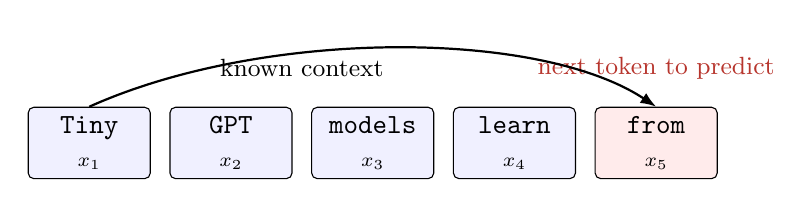
\begin{tikzpicture}[
  token/.style={draw, rounded corners=2pt, minimum width=1.55cm, minimum height=0.72cm, align=center},
  lab/.style={font=\small},
  arrow/.style={-{Latex[length=2mm]}, thick}
]
\node[token, fill=blue!6] (x1) at (0,0) {\texttt{Tiny}\\{\scriptsize \(x_1\)}};
\node[token, fill=blue!6] (x2) at (1.8,0) {\texttt{GPT}\\{\scriptsize \(x_2\)}};
\node[token, fill=blue!6] (x3) at (3.6,0) {\texttt{models}\\{\scriptsize \(x_3\)}};
\node[token, fill=blue!6] (x4) at (5.4,0) {\texttt{learn}\\{\scriptsize \(x_4\)}};
\node[token, fill=red!8] (target) at (7.2,0) {\texttt{from}\\{\scriptsize \(x_5\)}};
\node[lab] at (2.7,0.95) {known context};
\node[lab, text=maplered] at (7.2,0.95) {next token to predict};
\draw[arrow] (x1.north) .. controls (2.2,1.45) and (5.7,1.45) .. (target.north);
\end{tikzpicture}
\end{center}

In this example,
\[
P(x_5 \mid x_1,x_2,x_3,x_4)
= P(\texttt{from} \mid \texttt{Tiny},\texttt{GPT},\texttt{models},\texttt{learn}).
\]
This is the same formula, but now every symbol points to a real token.

The model is not given the future token while making the prediction. During training, we know the correct next token and use it to compute loss. During generation, we choose a next token from the model's predicted distribution and append it to the context.

\section{The Full Pipeline In One Picture}

\begin{center}
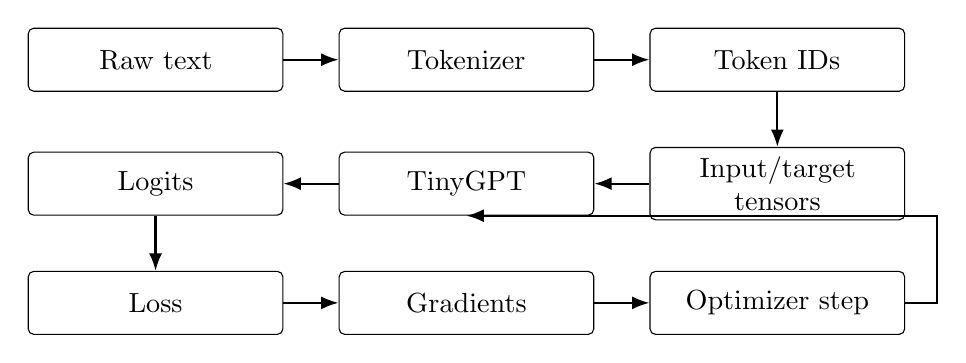
\begin{tikzpicture}[
  node distance=0.7cm,
  box/.style={draw, rounded corners=2pt, minimum height=0.8cm, text width=3.0cm, align=center},
  arrow/.style={-{Latex[length=2.2mm]}, thick}
]
\node[box] (text) {Raw text};
\node[box, right=of text] (tok) {Tokenizer};
\node[box, right=of tok] (ids) {Token IDs};
\node[box, below=of ids] (tensor) {Input/target tensors};
\node[box, left=of tensor] (model) {TinyGPT};
\node[box, left=of model] (logits) {Logits};
\node[box, below=of logits] (loss) {Loss};
\node[box, right=of loss] (grad) {Gradients};
\node[box, right=of grad] (opt) {Optimizer step};
\draw[arrow] (text) -- (tok);
\draw[arrow] (tok) -- (ids);
\draw[arrow] (ids) -- (tensor);
\draw[arrow] (tensor) -- (model);
\draw[arrow] (model) -- (logits);
\draw[arrow] (logits) -- (loss);
\draw[arrow] (loss) -- (grad);
\draw[arrow] (grad) -- (opt);
\draw[arrow] (opt.east) -- ++(0.4,0) |- (model.south);
\end{tikzpicture}
\end{center}

The same pipeline appears in every serious GPT training system:

\begin{lstlisting}
text -> tokenizer -> token ids -> tensors -> model
     -> logits -> loss -> gradients -> optimizer
     -> checkpoint -> sampling
\end{lstlisting}

The same pipeline also appears in source code. The table below is the first bridge between the mathematical idea, the TinyGPT data, and the software function that usually implements it.

\begin{longtable}{p{0.2\textwidth}p{0.25\textwidth}p{0.33\textwidth}}
\toprule
\term{Math idea} & \term{TinyGPT case} & \term{Code responsibility} \\
\midrule
Sequence \(x_1,\ldots,x_t\) & \texttt{Tiny GPT models learn} & store token IDs in a tensor \shape{[B,T]} \\
Vocabulary size \(V\) & 9 known tokens & tokenizer owns \texttt{vocab\_size} \\
Embedding matrix \(E\) & row 2 represents \texttt{Tiny} & \texttt{Embedding(V, C)} lookup \\
Model \(f_\theta(x)\) & TinyGPT forward pass & \texttt{model(x)} returns logits \\
Logits \(z\) & 9 scores for next token & final linear layer maps \(C \rightarrow V\) \\
Probability \(p_i\) & probability of \texttt{tokens} & softmax inside cross entropy or sampler \\
Loss \(-\log p_y\) & penalty for correct ID 7 & \texttt{cross\_entropy(logits, targets)} \\
Gradient \(\nabla_\theta L\) & parameter blame signal & \texttt{loss.backward()} \\
\bottomrule
\end{longtable}

The rest of the book explains each arrow carefully.

\section{Who Does What In A GPT Training System?}

It is helpful to treat TinyGPT training as a small factory. Each part has a job, an input, an output, and a failure mode. The mathematics is not separate from the software: the math defines the contract that each software part must satisfy.

\begin{center}
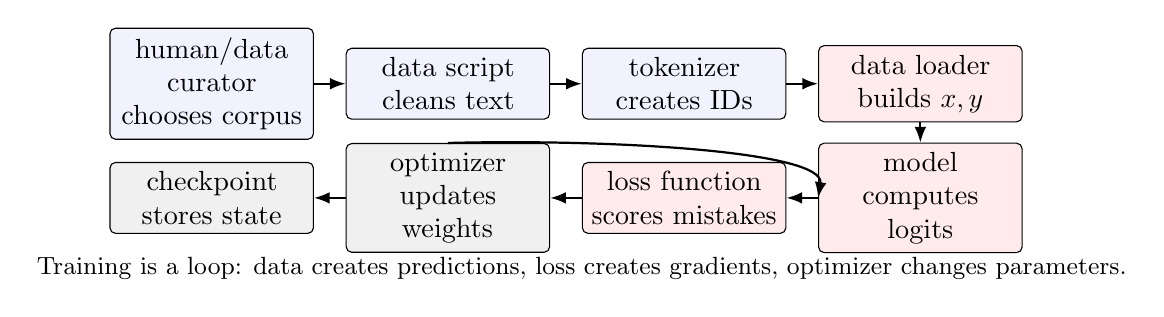
\begin{tikzpicture}[
  box/.style={draw, rounded corners=2pt, minimum height=0.72cm, text width=2.35cm, align=center},
  arrow/.style={-{Latex[length=2mm]}, thick},
  lab/.style={font=\small, align=center}
]
\node[box, fill=blue!5] (human) at (0,0) {human/data curator\\chooses corpus};
\node[box, fill=blue!5] (prep) at (3.0,0) {data script\\cleans text};
\node[box, fill=blue!5] (tok) at (6.0,0) {tokenizer\\creates IDs};
\node[box, fill=red!8] (loader) at (9.0,0) {data loader\\builds \(x,y\)};
\node[box, fill=red!8] (model) at (9.0,-1.45) {model\\computes logits};
\node[box, fill=red!8] (loss) at (6.0,-1.45) {loss function\\scores mistakes};
\node[box, fill=gray!12] (opt) at (3.0,-1.45) {optimizer\\updates weights};
\node[box, fill=gray!12] (ckpt) at (0,-1.45) {checkpoint\\stores state};
\draw[arrow] (human) -- (prep);
\draw[arrow] (prep) -- (tok);
\draw[arrow] (tok) -- (loader);
\draw[arrow] (loader) -- (model);
\draw[arrow] (model) -- (loss);
\draw[arrow] (loss) -- (opt);
\draw[arrow] (opt) -- (ckpt);
\draw[arrow] (opt.north) .. controls (5.0,-0.7) and (7.8,-0.85) .. (model.west);
\node[lab] at (4.7,-2.35) {Training is a loop: data creates predictions, loss creates gradients, optimizer changes parameters.};
\end{tikzpicture}
\end{center}

\begin{longtable}{p{0.18\textwidth}p{0.24\textwidth}p{0.24\textwidth}p{0.22\textwidth}}
\toprule
\term{Part} & \term{Receives} & \term{Produces} & \term{Main risk} \\
\midrule
Data curator & raw documents & approved corpus & bad or unsafe data \\
Tokenizer & text & token IDs & inconsistent vocabulary \\
Data loader & token stream & \(x,y\) batches & off-by-one target shift \\
Model & \(x\) & logits \(Z\) & wrong shapes or mask \\
Loss & logits and \(y\) & scalar \(L\) & wrong target alignment \\
Optimizer & gradients & new parameters & unstable learning rate \\
Checkpoint & states and config & resumable artifact & missing metadata \\
\bottomrule
\end{longtable}

This table is a practical debugging map. If generated text is poor, do not only blame the model. Check the whole chain: data, tokenizer, target shift, shapes, loss, optimizer, and checkpoint loading.

\section{The Four Views Of One Training Example}

The same TinyGPT example can be seen in four synchronized views.

\begin{center}
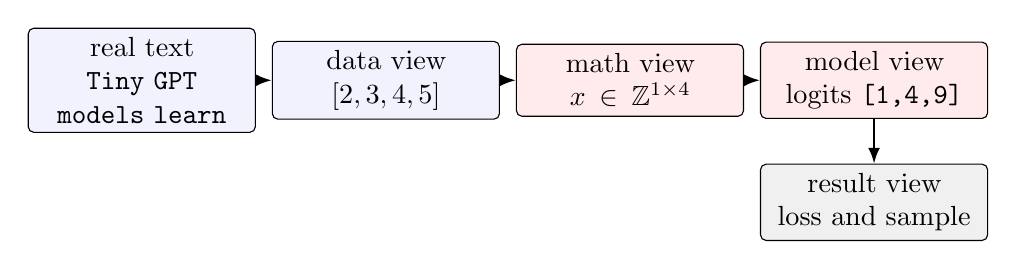
\begin{tikzpicture}[
  box/.style={draw, rounded corners=2pt, minimum height=0.85cm, text width=2.65cm, align=center},
  arrow/.style={-{Latex[length=2mm]}, thick}
]
\node[box, fill=blue!5] (real) at (0,0) {real text\\\texttt{Tiny GPT models learn}};
\node[box, fill=blue!5] (data) at (3.1,0) {data view\\\([2,3,4,5]\)};
\node[box, fill=red!8] (math) at (6.2,0) {math view\\\(x\in\mathbb{Z}^{1\times4}\)};
\node[box, fill=red!8] (model) at (9.3,0) {model view\\logits \shape{[1,4,9]}};
\node[box, fill=gray!12] (result) at (9.3,-1.55) {result view\\loss and sample};
\draw[arrow] (real) -- (data);
\draw[arrow] (data) -- (math);
\draw[arrow] (math) -- (model);
\draw[arrow] (model) -- (result);
\end{tikzpicture}
\end{center}

These views answer different questions:

\begin{itemize}
  \item The real-text view asks, ``What sentence are we teaching from?''
  \item The data view asks, ``What exact IDs enter the program?''
  \item The math view asks, ``What object and shape does the equation describe?''
  \item The model view asks, ``What tensor does the neural network produce?''
  \item The result view asks, ``Did the model assign probability to the correct next token?''
\end{itemize}

For a beginner, many GPT mistakes happen because these views become disconnected. A professional training workflow keeps them aligned.

\section{One Prediction, End To End}

The next diagram follows one supervised prediction through the whole system. The model sees the context ending in \texttt{from}; the target is \texttt{tokens}. This is the most important mental picture in the book.

\begin{center}
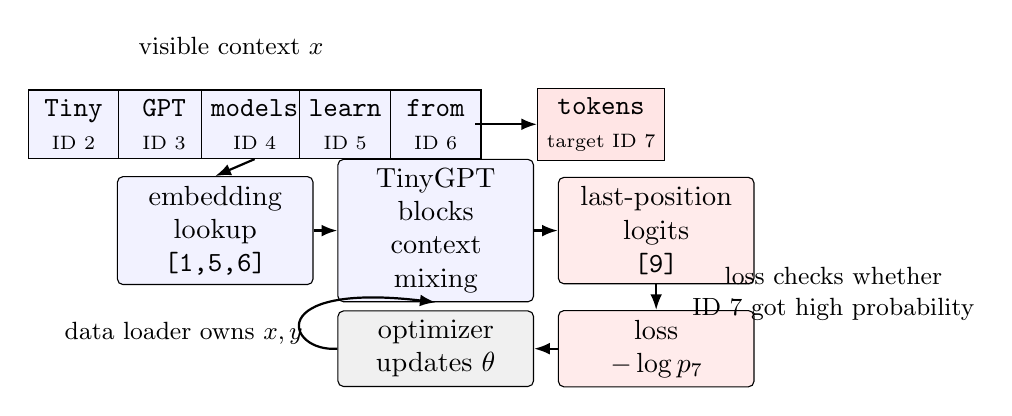
\begin{tikzpicture}[
  token/.style={draw, minimum width=1.15cm, minimum height=0.58cm, align=center},
  box/.style={draw, rounded corners=2pt, minimum height=0.72cm, text width=2.25cm, align=center},
  arrow/.style={-{Latex[length=2mm]}, thick},
  lab/.style={font=\small, align=center}
]
\node[lab] at (2.0,1.0) {visible context \(x\)};
\foreach \i/\tok/\id in {0/Tiny/2,1/GPT/3,2/models/4,3/learn/5,4/from/6} {
  \node[token, fill=blue!5] (t\i) at (\i*1.15,0) {\texttt{\tok}\\{\scriptsize ID \id}};
}
\node[token, fill=red!10] (target) at (6.7,0) {\texttt{tokens}\\{\scriptsize target ID 7}};
\draw[arrow] (5.1,0) -- (target);
\node[box, fill=blue!5] (embed) at (1.8,-1.35) {embedding lookup\\\shape{[1,5,6]}};
\node[box, fill=blue!5] (block) at (4.6,-1.35) {TinyGPT blocks\\context mixing};
\node[box, fill=red!8] (logits) at (7.4,-1.35) {last-position logits\\\shape{[9]}};
\node[box, fill=red!8] (loss) at (7.4,-2.85) {loss\\\(-\log p_7\)};
\node[box, fill=gray!12] (update) at (4.6,-2.85) {optimizer\\updates \(\theta\)};
\draw[arrow] (t2.south) -- (embed.north);
\draw[arrow] (embed) -- (block);
\draw[arrow] (block) -- (logits);
\draw[arrow] (logits) -- (loss);
\draw[arrow] (loss) -- (update);
\draw[arrow] (update.west) .. controls (2.7,-2.9) and (2.4,-2.0) .. (block.south);
\node[lab] at (1.4,-2.65) {data loader owns \(x,y\)};
\node[lab] at (9.65,-2.15) {loss checks whether\\ID 7 got high probability};
\end{tikzpicture}
\end{center}

The flow has five different kinds of objects:

\begin{longtable}{p{0.18\textwidth}p{0.26\textwidth}p{0.38\textwidth}}
\toprule
\term{Object} & \term{Example} & \term{Who manages it} \\
\midrule
Text & \texttt{Tiny GPT models learn from} & dataset and tokenizer code \\
IDs & \([2,3,4,5,6]\) & data loader \\
Vectors & \shape{[1,5,6]} & model embedding layer \\
Scores & logits \shape{[9]} & output head \\
Result & loss scalar & loss function and trainer \\
\bottomrule
\end{longtable}

This diagram is also the debugging order. If the result is wrong, inspect the IDs before the embeddings, inspect the embeddings before the logits, and inspect the logits before blaming the optimizer.

\section{Step 1: Raw Text}

The starting point is ordinary text:

\begin{quote}
\texttt{Tiny GPT models learn from tokens.}
\end{quote}

Text is easy for humans to read, but a neural network does not process words directly. Neural networks process arrays of numbers. Therefore, the first engineering problem is to convert text into numerical IDs.

\section{Step 2: Tokenization}

A \term{tokenizer} converts text into tokens. In a real GPT system, tokens may be words, word pieces, bytes, punctuation marks, or common character sequences. For this first chapter, use a simple word-level tokenizer so the idea is visible.

Assume the tokenizer learns this tiny vocabulary:

\begin{longtable}{p{0.24\textwidth}p{0.24\textwidth}p{0.34\textwidth}}
\toprule
\term{Token} & \term{ID} & \term{Comment} \\
\midrule
\texttt{MapleAI} & 0 & organization token \\
\texttt{trains} & 1 & verb \\
\texttt{Tiny} & 2 & adjective \\
\texttt{GPT} & 3 & model family token \\
\texttt{models} & 4 & noun \\
\texttt{learn} & 5 & verb \\
\texttt{from} & 6 & preposition \\
\texttt{tokens} & 7 & noun \\
\texttt{.} & 8 & punctuation \\
\bottomrule
\end{longtable}

Then the sentence

\begin{quote}
\texttt{Tiny GPT models learn from tokens .}
\end{quote}

might become:

\[
[2, 3, 4, 5, 6, 7, 8].
\]

The mapping can be drawn as a two-row strip:

\begin{center}
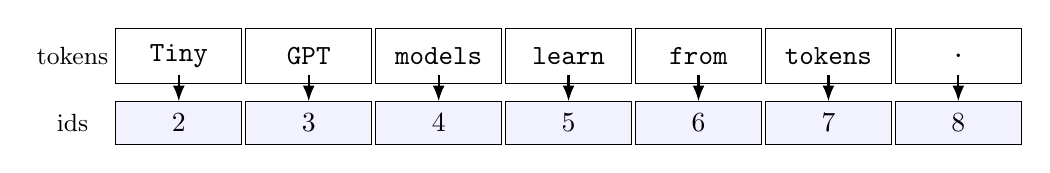
\begin{tikzpicture}[
  cell/.style={draw, minimum width=1.6cm, minimum height=0.7cm, align=center},
  idcell/.style={draw, minimum width=1.6cm, minimum height=0.55cm, align=center, fill=blue!5},
  arrow/.style={-{Latex[length=2mm]}, thick}
]
\node[cell] (t1) at (0,0) {\texttt{Tiny}};
\node[cell] (t2) at (1.65,0) {\texttt{GPT}};
\node[cell] (t3) at (3.3,0) {\texttt{models}};
\node[cell] (t4) at (4.95,0) {\texttt{learn}};
\node[cell] (t5) at (6.6,0) {\texttt{from}};
\node[cell] (t6) at (8.25,0) {\texttt{tokens}};
\node[cell] (t7) at (9.9,0) {\texttt{.}};
\node[idcell] at (0,-0.85) {2};
\node[idcell] at (1.65,-0.85) {3};
\node[idcell] at (3.3,-0.85) {4};
\node[idcell] at (4.95,-0.85) {5};
\node[idcell] at (6.6,-0.85) {6};
\node[idcell] at (8.25,-0.85) {7};
\node[idcell] at (9.9,-0.85) {8};
\node[align=right] at (-1.35,0) {\small tokens};
\node[align=right] at (-1.35,-0.85) {\small ids};
\foreach \x in {0,1.65,3.3,4.95,6.6,8.25,9.9}
  \draw[arrow] (\x,-0.25) -- (\x,-0.58);
\end{tikzpicture}
\end{center}

The exact token IDs are not meaningful by themselves. Token ID \(7\) is not mathematically ``larger'' than token ID \(3\) in a language sense. The ID is an index into a learned embedding table.

\section{Step 3: Input And Target Sequences}

GPT training uses shifted sequences. If the token stream is
\[
[2, 3, 4, 5, 6, 7, 8],
\]
and the context length is \(T=4\), then one training example can be:

\[
x = [2, 3, 4, 5],
\]
\[
y = [3, 4, 5, 6].
\]

The input \(x\) asks the model to predict:

\begin{longtable}{p{0.28\textwidth}p{0.28\textwidth}p{0.28\textwidth}}
\toprule
\term{Position} & \term{Context token} & \term{Target next token} \\
\midrule
0 & \texttt{Tiny} & \texttt{GPT} \\
1 & \texttt{GPT} & \texttt{models} \\
2 & \texttt{models} & \texttt{learn} \\
3 & \texttt{learn} & \texttt{from} \\
\bottomrule
\end{longtable}

This is the first essential GPT pattern:

\begin{lstlisting}
input:  token 0, token 1, token 2, token 3
target: token 1, token 2, token 3, token 4
\end{lstlisting}

Every target is the next token after the matching input position.

The shift is easier to see as parallel tracks:

\begin{center}
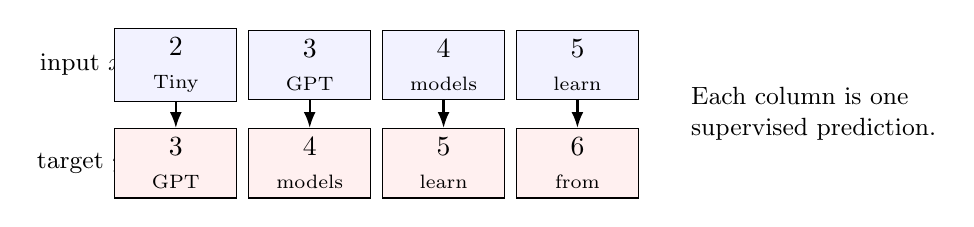
\begin{tikzpicture}[
  cell/.style={draw, minimum width=1.55cm, minimum height=0.62cm, align=center},
  incell/.style={cell, fill=blue!5},
  outcell/.style={cell, fill=red!6},
  lab/.style={font=\small},
  arrow/.style={-{Latex[length=2mm]}, thick}
]
\node[lab] at (-1.2,0) {input \(x\)};
\node[incell] (x0) at (0,0) {2\\{\scriptsize Tiny}};
\node[incell] (x1) at (1.7,0) {3\\{\scriptsize GPT}};
\node[incell] (x2) at (3.4,0) {4\\{\scriptsize models}};
\node[incell] (x3) at (5.1,0) {5\\{\scriptsize learn}};
\node[lab] at (-1.2,-1.25) {target \(y\)};
\node[outcell] (y0) at (0,-1.25) {3\\{\scriptsize GPT}};
\node[outcell] (y1) at (1.7,-1.25) {4\\{\scriptsize models}};
\node[outcell] (y2) at (3.4,-1.25) {5\\{\scriptsize learn}};
\node[outcell] (y3) at (5.1,-1.25) {6\\{\scriptsize from}};
\foreach \a/\b in {x0/y0,x1/y1,x2/y2,x3/y3}
  \draw[arrow] (\a.south) -- (\b.north);
\node[align=left, font=\small] at (8.1,-0.62) {Each column is one\\supervised prediction.};
\end{tikzpicture}
\end{center}

So the mathematical pair
\[
(x_t,y_t)=(x_t,x_{t+1})
\]
means something very concrete: the token currently visible at a position is used to predict the token immediately after it.

\section{Step 4: Tensors And Shapes}

Training uses batches. If batch size is \(B=2\) and context length is \(T=4\), the input tensor has shape
\[
x \in \mathbb{Z}^{2 \times 4}.
\]
For example:

\[
x =
\begin{bmatrix}
2 & 3 & 4 & 5 \\
0 & 1 & 2 & 3
\end{bmatrix},
\qquad
y =
\begin{bmatrix}
3 & 4 & 5 & 6 \\
1 & 2 & 3 & 4
\end{bmatrix}.
\]

The shape \shape{[B, T]} means:

\begin{itemize}
  \item \(B\): how many sequences are processed together;
  \item \(T\): how many token positions are in each sequence.
\end{itemize}

Shape reasoning is one of the most important practical skills in LLM training. If the shape is wrong, the mathematics is usually wrong too.

The batch can be read as a small spreadsheet of token IDs:

\begin{center}
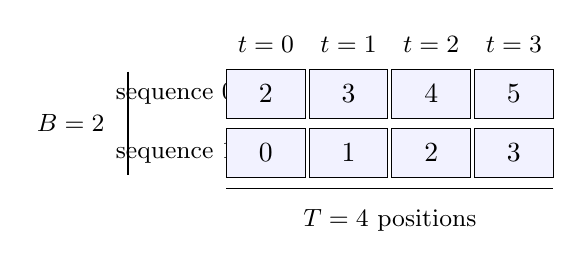
\begin{tikzpicture}[
  cell/.style={draw, minimum width=1.0cm, minimum height=0.62cm, align=center},
  rowlab/.style={font=\small, align=right},
  collab/.style={font=\small}
]
\node[rowlab] at (-1.15,0) {sequence 0};
\node[rowlab] at (-1.15,-0.75) {sequence 1};
\foreach \i/\v in {0/2,1/3,2/4,3/5}
  \node[cell, fill=blue!5] at (\i*1.05,0) {\v};
\foreach \i/\v in {0/0,1/1,2/2,3/3}
  \node[cell, fill=blue!5] at (\i*1.05,-0.75) {\v};
\foreach \i in {0,1,2,3}
  \node[collab] at (\i*1.05,0.62) {\(t=\i\)};
\draw[decorate] (-0.5,-1.2) -- node[below=4pt] {\small \(T=4\) positions} (3.65,-1.2);
\draw[decorate] (-1.75,0.28) -- node[left=5pt] {\small \(B=2\)} (-1.75,-1.03);
\end{tikzpicture}
\end{center}

The notation \(x \in \mathbb{Z}^{2 \times 4}\) is just the mathematical way of saying ``two rows, four token IDs per row.''

\section{Step 5: Embeddings}

Token IDs are indices. The model must convert them into vectors. If the vocabulary size is \(V=9\) and the embedding dimension is \(C=6\), then the token embedding table has shape
\[
E_{\text{tok}} \in \mathbb{R}^{9 \times 6}.
\]

Each token ID selects one row. After embedding, the tensor shape changes:

\[
\shape{[B, T]} \rightarrow \shape{[B, T, C]}.
\]

For our sample:

\[
\shape{[2, 4]} \rightarrow \shape{[2, 4, 6]}.
\]

This means each token position is now represented by a vector of six learned numbers. Real GPT models use much larger dimensions, such as 768, 1024, or more.

The embedding lookup is not a calculation like \(2 \times 6\). It is a table lookup:

\begin{center}
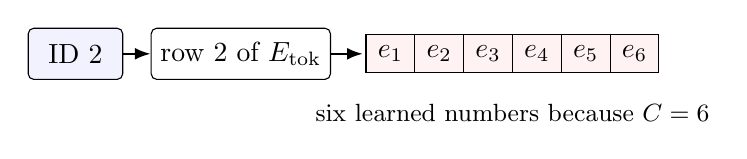
\begin{tikzpicture}[
  small/.style={draw, minimum width=0.62cm, minimum height=0.48cm, align=center},
  box/.style={draw, rounded corners=2pt, minimum width=1.2cm, minimum height=0.65cm, align=center},
  arrow/.style={-{Latex[length=2mm]}, thick}
]
\node[box, fill=blue!5] (id) at (0,0) {ID 2};
\node[box] (row) at (2.1,0) {row 2 of \(E_{\text{tok}}\)};
\node[small, fill=red!5] at (4.0,0) {\(e_1\)};
\node[small, fill=red!5] at (4.62,0) {\(e_2\)};
\node[small, fill=red!5] at (5.24,0) {\(e_3\)};
\node[small, fill=red!5] at (5.86,0) {\(e_4\)};
\node[small, fill=red!5] at (6.48,0) {\(e_5\)};
\node[small, fill=red!5] at (7.10,0) {\(e_6\)};
\draw[arrow] (id) -- (row);
\draw[arrow] (row) -- (3.65,0);
\node[font=\small, align=center] at (5.55,-0.75) {six learned numbers because \(C=6\)};
\end{tikzpicture}
\end{center}

After this lookup, token \texttt{Tiny} is no longer just ID \(2\). It is a vector that the model can add, multiply, compare, and update during training.

\section{Step 6: The Transformer}

The Transformer is the main model body. It repeatedly applies two ideas:

\begin{itemize}
  \item \term{attention}: each position reads information from previous positions;
  \item \term{feed-forward transformation}: each position's vector is transformed through learned linear layers and nonlinearities.
\end{itemize}

A causal GPT model can use tokens on the left, but not tokens on the right. When predicting the token after \texttt{models}, the model can use:

\begin{quote}
\texttt{Tiny GPT models}
\end{quote}

but not:

\begin{quote}
\texttt{learn from tokens}
\end{quote}

because those are future tokens relative to that prediction.

For the context \texttt{Tiny GPT models learn}, causal attention allows this reading pattern:

\begin{center}
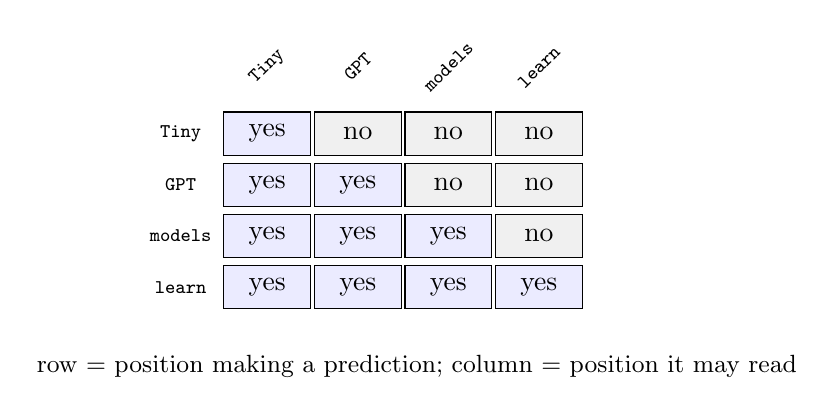
\begin{tikzpicture}[
  cell/.style={draw, minimum width=1.1cm, minimum height=0.55cm, align=center},
  yes/.style={cell, fill=blue!8},
  no/.style={cell, fill=gray!12},
  lab/.style={font=\scriptsize}
]
\foreach \i/\name in {0/Tiny,1/GPT,2/models,3/learn} {
  \node[lab, rotate=45] at (\i*1.15+1.1,0.55) {\texttt{\name}};
  \node[lab] at (0,\i*-0.65-0.3) {\texttt{\name}};
}
\foreach \r in {0,1,2,3} {
  \foreach \c in {0,1,2,3} {
    \ifnum\c>\r
      \node[no] at (\c*1.15+1.1,\r*-0.65-0.3) {no};
    \else
      \node[yes] at (\c*1.15+1.1,\r*-0.65-0.3) {yes};
    \fi
  }
}
\node[font=\small, align=center] at (3.0,-3.25) {row = position making a prediction; column = position it may read};
\end{tikzpicture}
\end{center}

The lower-triangular pattern is the visual form of ``no future tokens.'' This is why GPT can be trained on complete text while still learning a left-to-right generation rule.

\section{Step 7: Logits}

The model outputs \term{logits}. A logit is a raw score before probability normalization. For each position, the model produces one score for every vocabulary token.

If \(B=2\), \(T=4\), and \(V=9\), then logits have shape:

\[
\shape{[2, 4, 9]}.
\]

At each position, the model is saying:

\begin{quote}
Here are my nine scores for the next token.
\end{quote}

Softmax converts those scores into probabilities:

\[
p_i = \frac{e^{z_i}}{\sum_{j=1}^{V} e^{z_j}}.
\]

Here is a concrete example for one position. Suppose the model has seen:

\begin{quote}
\texttt{Tiny GPT models learn from}
\end{quote}

The correct next token is \texttt{tokens}, ID \(7\). TinyGPT produces one logit for every vocabulary token:

\begin{center}
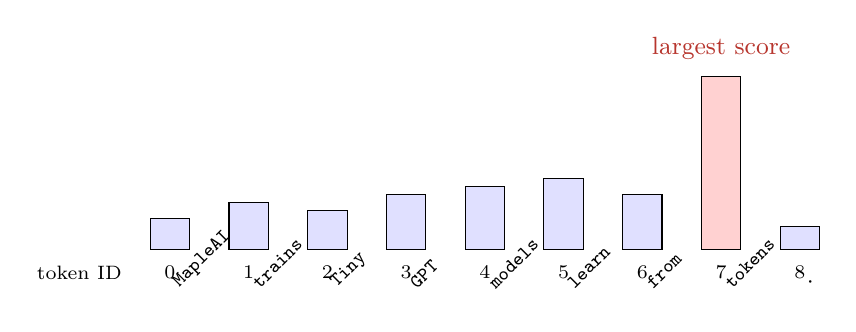
\begin{tikzpicture}[
  bar/.style={draw, fill=blue!12, minimum height=0.45cm},
  targ/.style={draw, fill=red!18, minimum height=0.45cm},
  lab/.style={font=\scriptsize}
]
\node[lab, align=right] at (-1.15,0) {token ID};
\foreach \i/\w/\h in {0/MapleAI/0.4,1/trains/0.6,2/Tiny/0.5,3/GPT/0.7,4/models/0.8,5/learn/0.9,6/from/0.7,7/tokens/2.2,8/./0.3} {
  \node[lab] at (\i*1.0,0) {\i};
  \node[lab, rotate=45, anchor=west] at (\i*1.0,-0.25) {\texttt{\w}};
  \ifnum\i=7
    \node[targ, anchor=south, minimum width=0.5cm, minimum height=\h cm] at (\i*1.0,0.28) {};
  \else
    \node[bar, anchor=south, minimum width=0.5cm, minimum height=\h cm] at (\i*1.0,0.28) {};
  \fi
}
\node[font=\small, text=maplered] at (7,2.85) {largest score};
\end{tikzpicture}
\end{center}

If softmax turns these logits into \(p_{\texttt{tokens}}=0.64\), then the model assigns \(64\%\) probability to the correct next token at this position.

The full shape story from input IDs to logits is:

\begin{center}
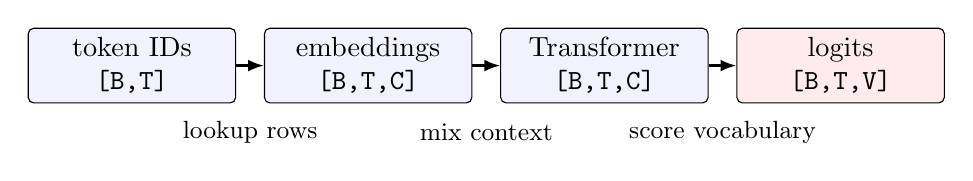
\begin{tikzpicture}[
  box/.style={draw, rounded corners=2pt, minimum height=0.75cm, text width=2.4cm, align=center},
  arrow/.style={-{Latex[length=2mm]}, thick},
  note/.style={font=\small, align=center}
]
\node[box, fill=blue!5] (ids) at (0,0) {token IDs\\\shape{[B,T]}};
\node[box, fill=blue!5] (emb) at (3.0,0) {embeddings\\\shape{[B,T,C]}};
\node[box, fill=blue!5] (blocks) at (6.0,0) {Transformer\\\shape{[B,T,C]}};
\node[box, fill=red!8] (logits) at (9.0,0) {logits\\\shape{[B,T,V]}};
\draw[arrow] (ids) -- (emb);
\draw[arrow] (emb) -- (blocks);
\draw[arrow] (blocks) -- (logits);
\node[note] at (1.5,-0.85) {lookup rows};
\node[note] at (4.5,-0.85) {mix context};
\node[note] at (7.5,-0.85) {score vocabulary};
\end{tikzpicture}
\end{center}

For TinyGPT in this chapter, \(B=2\), \(T=4\), \(C=6\), and \(V=9\). Therefore:

\[
\shape{[2,4]} \rightarrow \shape{[2,4,6]} \rightarrow \shape{[2,4,6]} \rightarrow \shape{[2,4,9]}.
\]

The middle shape stays \shape{[B,T,C]} because Transformer blocks change the content of each vector, not the number of sequences, positions, or channels.

\section{Step 8: Loss}

The training loss measures how surprised the model is by the correct next token. If the correct next token is \(y\), and the model assigns probability \(p_y\), then the loss for that prediction is:

\[
\ell = -\log p_y.
\]

If the model assigns high probability to the correct token, the loss is small. If it assigns low probability to the correct token, the loss is large.

For the concrete \texttt{tokens} example:

\[
y = 7,\qquad p_y = p_{\texttt{tokens}} = 0.64.
\]

The loss is:

\[
\ell = -\log(0.64) \approx 0.446.
\]

If the model had assigned only \(p_y=0.05\), the loss would be:

\[
\ell = -\log(0.05) \approx 2.996.
\]

So the loss is not a mysterious score. It is a numerical penalty for not trusting the correct next token enough.

\begin{center}
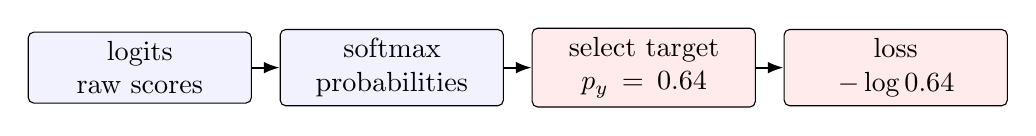
\begin{tikzpicture}[
  box/.style={draw, rounded corners=2pt, minimum height=0.7cm, text width=2.6cm, align=center},
  arrow/.style={-{Latex[length=2mm]}, thick}
]
\node[box, fill=blue!5] (logits) at (0,0) {logits\\raw scores};
\node[box, fill=blue!5] (softmax) at (3.2,0) {softmax\\probabilities};
\node[box, fill=red!8] (pick) at (6.4,0) {select target\\\(p_y=0.64\)};
\node[box, fill=red!8] (loss) at (9.6,0) {loss\\\(-\log 0.64\)};
\draw[arrow] (logits) -- (softmax);
\draw[arrow] (softmax) -- (pick);
\draw[arrow] (pick) -- (loss);
\end{tikzpicture}
\end{center}

For a batch, the cross-entropy loss averages over all \(B \times T\) predictions:

\[
L = -\frac{1}{BT}\sum_{b=1}^{B}\sum_{t=1}^{T}\log p_{b,t,y_{b,t}}.
\]

\section{Step 9: Gradients And The Optimizer}

The model contains parameters: embedding rows, attention matrices, feed-forward matrices, normalization weights, and output weights. Training means changing those parameters to reduce loss.

Backpropagation computes the gradient:

\[
\nabla_{\theta} L.
\]

The optimizer updates the parameters. A simple gradient descent update is:

\[
\theta_{\text{new}} = \theta_{\text{old}} - \eta \nabla_{\theta}L,
\]

where \(\eta\) is the learning rate. Real training often uses AdamW rather than plain gradient descent, but the principle is the same: use the gradient to change parameters in a direction that tends to reduce loss.

\section{Step 10: Checkpoints And Sampling}

A \term{checkpoint} saves training state. A useful checkpoint includes:

\begin{itemize}
  \item model weights;
  \item optimizer state;
  \item model config;
  \item tokenizer identity;
  \item current training step;
  \item random seed or random number generator states when possible.
\end{itemize}

After training, we can sample from the model. Sampling starts with a prompt:

\begin{quote}
\texttt{Tiny GPT}
\end{quote}

The model predicts a distribution for the next token. We choose one token, append it, and repeat:

\begin{lstlisting}
Tiny GPT
Tiny GPT models
Tiny GPT models learn
Tiny GPT models learn from
Tiny GPT models learn from tokens
\end{lstlisting}

This is generation. It is still next-token prediction, used repeatedly.

\section{TinyGPT Source Code Logic}

Now we connect the same ideas to code. This is not yet a production implementation. It is a readable teaching skeleton. The purpose is to understand how every mathematical object becomes a software object.

\subsection{Code Map}

\begin{center}
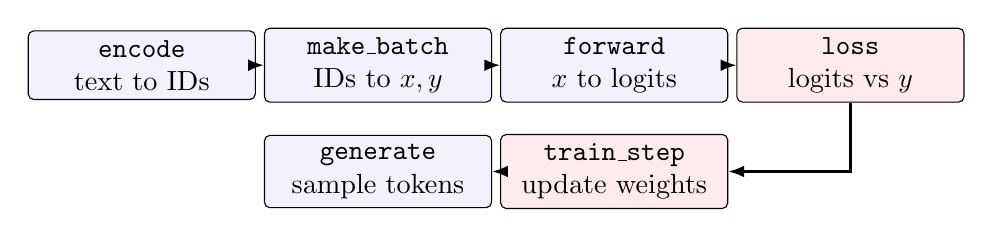
\begin{tikzpicture}[
  box/.style={draw, rounded corners=2pt, minimum height=0.75cm, text width=2.65cm, align=center},
  arrow/.style={-{Latex[length=2mm]}, thick}
]
\node[box, fill=blue!5] (tok) at (0,0) {\texttt{encode}\\text to IDs};
\node[box, fill=blue!5] (batch) at (3.0,0) {\texttt{make\_batch}\\IDs to \(x,y\)};
\node[box, fill=blue!5] (forward) at (6.0,0) {\texttt{forward}\\\(x\) to logits};
\node[box, fill=red!8] (loss) at (9.0,0) {\texttt{loss}\\logits vs \(y\)};
\node[box, fill=red!8] (step) at (6.0,-1.35) {\texttt{train\_step}\\update weights};
\node[box, fill=blue!5] (gen) at (3.0,-1.35) {\texttt{generate}\\sample tokens};
\draw[arrow] (tok) -- (batch);
\draw[arrow] (batch) -- (forward);
\draw[arrow] (forward) -- (loss);
\draw[arrow] (loss) |- (step);
\draw[arrow] (step) -- (gen);
\end{tikzpicture}
\end{center}

Read this diagram left to right. The tokenizer prepares numbers. The batch function creates supervised examples. The model forward pass computes logits. The loss compares those logits to targets. The training step updates weights. Generation uses the trained model repeatedly.

\subsection{Tokenizer Functions}

The tokenizer owns the vocabulary. In this first chapter we use a tiny word-level tokenizer:

\begin{lstlisting}[language=Python]
token_to_id = {
    "MapleAI": 0,
    "trains": 1,
    "Tiny": 2,
    "GPT": 3,
    "models": 4,
    "learn": 5,
    "from": 6,
    "tokens": 7,
    ".": 8,
}
id_to_token = {i: tok for tok, i in token_to_id.items()}

def encode(text):
    tokens = text.split()
    return [token_to_id[tok] for tok in tokens]

def decode(ids):
    tokens = [id_to_token[i] for i in ids]
    return " ".join(tokens)
\end{lstlisting}

\term{What the code does}: \texttt{encode()} maps visible text tokens to integer IDs. \texttt{decode()} maps IDs back to text tokens.

\term{How this maps to math}: the vocabulary is the set \(\{0,\ldots,V-1\}\). Here \(V=9\). The token sequence
\[
[\texttt{Tiny},\texttt{GPT},\texttt{models},\texttt{learn},\texttt{from},\texttt{tokens},\texttt{.}]
\]
becomes
\[
[2,3,4,5,6,7,8].
\]

\term{Why it works}: neural networks need numeric inputs. The tokenizer creates a stable contract between text and numbers. If this contract changes, the model weights no longer mean the same thing.

\subsection{Batch Function}

The batch function creates \(x\) and \(y\). The important idea is the one-token shift.

\begin{lstlisting}[language=Python]
def make_one_example(ids, start, block_size):
    chunk = ids[start : start + block_size + 1]
    x = chunk[:-1]
    y = chunk[1:]
    return x, y
\end{lstlisting}

For:

\begin{lstlisting}
ids = [2, 3, 4, 5, 6, 7, 8]
block_size = 4
start = 0
\end{lstlisting}

the chunk is:

\[
[2,3,4,5,6].
\]

Then:

\[
x=[2,3,4,5],
\qquad
y=[3,4,5,6].
\]

\begin{center}
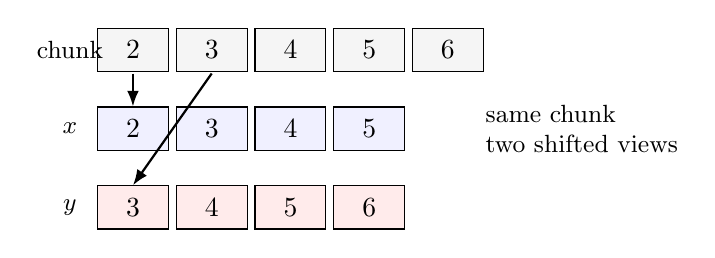
\begin{tikzpicture}[
  cell/.style={draw, minimum width=0.9cm, minimum height=0.55cm, align=center},
  arrow/.style={-{Latex[length=2mm]}, thick},
  lab/.style={font=\small}
]
\foreach \i/\v in {0/2,1/3,2/4,3/5,4/6} {
  \node[cell, fill=gray!8] at (\i*1.0,0) {\v};
}
\node[lab] at (-0.8,0) {chunk};
\foreach \i/\v in {0/2,1/3,2/4,3/5} {
  \node[cell, fill=blue!6] at (\i*1.0,-1.0) {\v};
}
\node[lab] at (-0.8,-1.0) {\(x\)};
\foreach \i/\v in {0/3,1/4,2/5,3/6} {
  \node[cell, fill=red!8] at (\i*1.0,-2.0) {\v};
}
\node[lab] at (-0.8,-2.0) {\(y\)};
\draw[arrow] (0,-0.3) -- (0,-0.72);
\draw[arrow] (1,-0.3) -- (0,-1.72);
\node[lab, align=left] at (5.7,-1.0) {same chunk\\two shifted views};
\end{tikzpicture}
\end{center}

\term{Why the function needs \texttt{block\_size + 1}}: to build \(T\) input tokens and \(T\) target tokens, the loader needs one extra future token. Without the extra token, the final input position would not have a target.

\subsection{Model Configuration}

A model config records the sizes that appear in the math:

\begin{lstlisting}[language=Python]
config = {
    "vocab_size": 9,    # V
    "block_size": 4,    # T
    "n_embd": 6,        # C
    "n_layer": 2,
    "n_head": 2,
}
\end{lstlisting}

This tiny config means:

\begin{longtable}{p{0.22\textwidth}p{0.2\textwidth}p{0.42\textwidth}}
\toprule
\term{Config} & \term{Symbol} & \term{Meaning} \\
\midrule
\texttt{vocab\_size} & \(V=9\) & nine possible next-token classes \\
\texttt{block\_size} & \(T=4\) & four context positions per example \\
\texttt{n\_embd} & \(C=6\) & each token becomes a six-number vector \\
\texttt{n\_layer} & 2 & two Transformer blocks \\
\texttt{n\_head} & 2 & two attention heads per block \\
\bottomrule
\end{longtable}

\term{Why config matters}: source code should not hide model dimensions. If the checkpoint says the output head has shape \(6 \times 9\), the config must explain that \(C=6\) and \(V=9\).

\subsection{The TinyGPT Module}

A GPT model is a function with parameters:

\[
f_\theta(x) = \text{logits}.
\]

In PyTorch-style code, that idea becomes a class:

\begin{lstlisting}[language=Python]
class TinyGPT(nn.Module):
    def __init__(self, config):
        super().__init__()
        V = config["vocab_size"]
        T = config["block_size"]
        C = config["n_embd"]

        self.token_emb = nn.Embedding(V, C)
        self.pos_emb = nn.Embedding(T, C)
        self.blocks = nn.ModuleList([
            TransformerBlock(config)
            for _ in range(config["n_layer"])
        ])
        self.ln_f = nn.LayerNorm(C)
        self.lm_head = nn.Linear(C, V)
\end{lstlisting}

\term{Block by block}:

\begin{itemize}
  \item \texttt{token\_emb}: maps token IDs to vectors, \(V \rightarrow C\).
  \item \texttt{pos\_emb}: gives each position \(0,\ldots,T-1\) its own vector.
  \item \texttt{blocks}: repeated Transformer blocks that mix context.
  \item \texttt{ln\_f}: final normalization for stable hidden states.
  \item \texttt{lm\_head}: maps each hidden vector back to \(V\) logits.
\end{itemize}

Visually:

\begin{center}
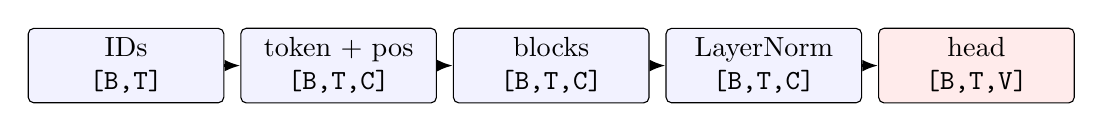
\begin{tikzpicture}[
  box/.style={draw, rounded corners=2pt, minimum height=0.75cm, text width=2.25cm, align=center},
  arrow/.style={-{Latex[length=2mm]}, thick}
]
\node[box, fill=blue!5] (id) at (0,0) {IDs\\\shape{[B,T]}};
\node[box, fill=blue!5] (emb) at (2.7,0) {token + pos\\\shape{[B,T,C]}};
\node[box, fill=blue!5] (blk) at (5.4,0) {blocks\\\shape{[B,T,C]}};
\node[box, fill=blue!5] (ln) at (8.1,0) {LayerNorm\\\shape{[B,T,C]}};
\node[box, fill=red!8] (head) at (10.8,0) {head\\\shape{[B,T,V]}};
\draw[arrow] (id) -- (emb);
\draw[arrow] (emb) -- (blk);
\draw[arrow] (blk) -- (ln);
\draw[arrow] (ln) -- (head);
\end{tikzpicture}
\end{center}

\subsection{Forward Function}

The \texttt{forward()} function tells us how data moves through the model:

\begin{lstlisting}[language=Python]
def forward(self, idx, targets=None):
    B, T = idx.shape
    positions = torch.arange(T, device=idx.device)

    tok = self.token_emb(idx)        # [B, T, C]
    pos = self.pos_emb(positions)    # [T, C]
    x = tok + pos                    # [B, T, C]

    for block in self.blocks:
        x = block(x)                 # [B, T, C]

    x = self.ln_f(x)                 # [B, T, C]
    logits = self.lm_head(x)         # [B, T, V]

    if targets is None:
        return logits, None

    loss = F.cross_entropy(
        logits.view(B*T, -1),
        targets.view(B*T),
    )
    return logits, loss
\end{lstlisting}

\term{Line by line}:

\begin{itemize}
  \item \texttt{B, T = idx.shape}: reads the batch and context dimensions.
  \item \texttt{positions}: creates \([0,1,2,3]\) for a four-token context.
  \item \texttt{token\_emb(idx)}: maps token IDs to vectors.
  \item \texttt{pos\_emb(positions)}: maps positions to vectors.
  \item \texttt{x = tok + pos}: combines identity and order.
  \item \texttt{block(x)}: lets positions read previous positions and transform features.
  \item \texttt{lm\_head(x)}: produces vocabulary scores.
  \item \texttt{cross\_entropy}: compares all \([B,T]\) predictions with all \([B,T]\) targets.
\end{itemize}

The reshape in the loss is important. PyTorch cross entropy expects a table of predictions:

\[
\shape{[B,T,V]} \rightarrow \shape{[B T,V]},
\]
and target labels:
\[
\shape{[B,T]} \rightarrow \shape{[B T]}.
\]

For TinyGPT, this means:

\[
\shape{[2,4,9]} \rightarrow \shape{[8,9]},
\qquad
\shape{[2,4]} \rightarrow \shape{[8]}.
\]

The model made eight predictions, and each prediction has nine possible classes.

\subsection{Training Step}

One training step connects loss to parameter updates:

\begin{lstlisting}[language=Python]
def train_step(model, optimizer, x, y):
    logits, loss = model(x, y)
    optimizer.zero_grad(set_to_none=True)
    loss.backward()
    optimizer.step()
    return loss.item()
\end{lstlisting}

\term{Why each line exists}:

\begin{itemize}
  \item \texttt{model(x,y)} computes logits and loss.
  \item \texttt{zero\_grad()} clears old gradients.
  \item \texttt{loss.backward()} computes \(\nabla_\theta L\).
  \item \texttt{optimizer.step()} changes \(\theta\).
  \item \texttt{return loss.item()} records a human-readable number.
\end{itemize}

The mathematical update
\[
\theta_{\text{new}} = \theta_{\text{old}} - \eta \nabla_\theta L
\]
is implemented inside \texttt{optimizer.step()}. AdamW uses a more sophisticated version of this update, but it still uses gradients computed from the loss.

\subsection{Generation Function}

Generation uses the same model, but without targets:

\begin{lstlisting}[language=Python]
def generate(model, prompt_ids, max_new_tokens):
    ids = prompt_ids[:]
    for _ in range(max_new_tokens):
        context = ids[-model.block_size:]
        x = torch.tensor([context])
        logits, _ = model(x)
        next_logits = logits[0, -1, :]
        probs = torch.softmax(next_logits, dim=-1)
        next_id = torch.multinomial(probs, num_samples=1).item()
        ids.append(next_id)
    return ids
\end{lstlisting}

\term{How it works}:

\begin{enumerate}
  \item Keep the latest context tokens.
  \item Run the model forward.
  \item Use only the last position's logits.
  \item Convert logits to probabilities.
  \item Sample one next token.
  \item Append it and repeat.
\end{enumerate}

Training and generation are the same next-token idea in two modes:

\begin{longtable}{p{0.22\textwidth}p{0.3\textwidth}p{0.3\textwidth}}
\toprule
\term{Mode} & \term{Known} & \term{Action} \\
\midrule
Training & correct target \(y\) & compute loss and update weights \\
Generation & no target \(y\) & choose a next token and append it \\
\bottomrule
\end{longtable}

\section{The Minimal GPT Training Contract}

A training repository needs clear contracts between parts. The following table is the first professional version of the system.

\begin{longtable}{p{0.24\textwidth}p{0.64\textwidth}}
\toprule
\term{Component} & \term{Responsibility} \\
\midrule
Tokenizer & Converts text to token IDs and token IDs back to text. Defines \(V\). \\
Dataset reader & Produces input tensor \shape{[B, T]} and target tensor \shape{[B, T]}. \\
Model & Maps token IDs to logits of shape \shape{[B, T, V]}. \\
Loss & Compares logits with targets using cross entropy. \\
Optimizer & Updates trainable parameters using gradients. \\
Checkpoint & Stores model state, optimizer state, config, tokenizer identity, and step. \\
Sampler & Generates text by repeatedly selecting the next token. \\
\bottomrule
\end{longtable}

The model may be implemented in PyTorch, Rust/Candle, or C/CUDA. The contract should remain the same.

\section{Why We Start Small}

Students often want to train a famous model immediately. That is understandable. But large models are bad first debugging tools. If a 124M-parameter model has a target-shifting bug, it may waste hours of GPU time before the problem is obvious.

The correct first milestones are:

\begin{enumerate}
  \item Run a tokenizer round trip: text to IDs to text.
  \item Build one input/target batch.
  \item Verify tensor shapes.
  \item Run one forward pass.
  \item Compute one loss.
  \item Overfit one tiny batch.
  \item Save and reload one checkpoint.
  \item Generate a short sample.
\end{enumerate}

Only after these work should the model size and dataset size increase.

\engineering

For a real training pack, Chapter 1 implies these project artifacts:

\begin{lstlisting}
configs/
  tiny_gpt_smoke.yaml
data/
  tokens/
scripts/
  prepare_tokens.py
  train_torch.py
  sample_torch.py
  inspect_tokens.py
backends/
  torch_reference/
  candle_rust/
  llmc_cuda/
checkpoints/
docs/
\end{lstlisting}

The names matter. \texttt{torch\_reference} means the PyTorch path is the readable teaching implementation. \texttt{candle\_rust} means the Rust path is a backend, not a separate project. \texttt{llmc\_cuda} means a low-level backend or comparison path, not the whole training pack.

\labtitle{Trace TinyGPT End To End}

Use this sentence:

\begin{quote}
\texttt{Tiny GPT models learn from tokens .}
\end{quote}

Use the vocabulary table from this chapter.

\begin{enumerate}
  \item Convert the sentence to token IDs.
  \item With context length \(T=4\), write one input row \(x\) and one target row \(y\).
  \item If \(B=1\), \(T=4\), \(C=6\), and \(V=9\), write the shapes of:
    \begin{itemize}
      \item input IDs;
      \item embedded vectors;
      \item logits;
      \item target IDs.
    \end{itemize}
  \item Explain, in one paragraph, why the target is shifted by one token.
\end{enumerate}

\section{Chapter Questions}

\begin{enumerate}
  \item What probability does a GPT-style next-token model estimate?
  \item In the sample vocabulary, what token ID represents \texttt{models}?
  \item Why are token IDs not meaningful numerical quantities by themselves?
  \item If \(B=2\), \(T=4\), and \(V=9\), what is the shape of the logits tensor?
  \item Why does the target tensor shift the input sequence by one position?
  \item What is the difference between logits and probabilities?
  \item What does the cross-entropy loss measure?
  \item Why should a tiny overfit test happen before a large training run?
  \item What information should be saved in a checkpoint besides model weights?
  \item Why can the same GPT architecture have PyTorch, Candle, and C/CUDA backends?
\end{enumerate}

\section{Solutions}

\begin{enumerate}
  \item A GPT-style next-token model estimates
  \[
  P(x_{t+1} \mid x_1, x_2, \ldots, x_t).
  \]
  In words, it estimates the probability distribution of the next token given all previous tokens in the context.

  \item In the sample vocabulary, \texttt{models} has token ID \(4\).

  \item Token IDs are arbitrary indices into a vocabulary or embedding table. ID \(7\) is not semantically greater than ID \(3\). The meaning is learned in the embedding vectors and later model layers.

  \item The logits tensor has shape \shape{[2, 4, 9]}. There are two sequences, four positions per sequence, and nine vocabulary scores at each position.

  \item The target shifts by one position because each input token position is trained to predict the next token. If the input is \([2,3,4,5]\), the target is \([3,4,5,6]\).

  \item Logits are raw model scores. Probabilities are normalized values after softmax. Probabilities are nonnegative and sum to one; logits can be any real numbers.

  \item Cross-entropy measures how much probability the model assigned to the correct token. Low probability for the correct token gives high loss; high probability gives low loss.

  \item A tiny overfit test checks whether the training path can actually learn. If the model cannot memorize one tiny batch, a larger run is likely hiding a bug in data loading, target shifting, loss computation, optimizer setup, or model code.

  \item A good checkpoint also saves optimizer state, model config, tokenizer identity, current step, and random state when possible. This allows training to resume and makes the checkpoint interpretable.

  \item The architecture is a mathematical and engineering contract: token IDs go in, logits come out, and loss is computed against shifted targets. PyTorch, Candle, and C/CUDA can all implement that same contract with different tradeoffs in readability, deployment, and performance.
\end{enumerate}

\section{Lab Solution}

For the sentence:

\begin{quote}
\texttt{Tiny GPT models learn from tokens .}
\end{quote}

the token IDs are:

\[
[2, 3, 4, 5, 6, 7, 8].
\]

With \(T=4\), one possible input row and target row are:

\[
x = [2, 3, 4, 5],
\qquad
y = [3, 4, 5, 6].
\]

If \(B=1\), \(T=4\), \(C=6\), and \(V=9\), the shapes are:

\begin{longtable}{p{0.34\textwidth}p{0.34\textwidth}}
\toprule
\term{Object} & \term{Shape} \\
\midrule
input IDs & \shape{[1, 4]} \\
embedded vectors & \shape{[1, 4, 6]} \\
logits & \shape{[1, 4, 9]} \\
target IDs & \shape{[1, 4]} \\
\bottomrule
\end{longtable}

The target is shifted because GPT training asks every position to predict the next token. The model sees token \texttt{Tiny} at the first position and is trained to predict \texttt{GPT}; it sees \texttt{GPT} at the second position and is trained to predict \texttt{models}; and so on. This creates many supervised predictions from one sequence.

\chapter{Mathematical Foundations For TinyGPT}

Chapter 1 showed the whole TinyGPT pipeline. This chapter slows down and builds the mathematical tools behind that pipeline. The purpose is not abstract mathematics for its own sake. Every symbol in this chapter will be connected to the TinyGPT sample case, to tensor shapes, and to source-code operations.

\section{Chapter Goals}

By the end of this chapter, you should be able to:

\begin{itemize}
  \item distinguish scalars, vectors, matrices, and tensors in a GPT model;
  \item map TinyGPT token data to mathematical shapes;
  \item explain matrix multiplication as the core operation inside linear layers;
  \item compute softmax and cross-entropy loss for one TinyGPT prediction;
  \item explain gradients as directions for changing model parameters;
  \item read simple source-code functions for linear layers, softmax, loss, and gradient updates.
\end{itemize}

\section{The Running TinyGPT Example}

We keep the same sample sentence:

\begin{quote}
\texttt{Tiny GPT models learn from tokens .}
\end{quote}

Using the Chapter 1 vocabulary, this becomes:

\[
[2,3,4,5,6,7,8].
\]

With context length \(T=4\), one input-target pair is:

\[
x=[2,3,4,5],
\qquad
y=[3,4,5,6].
\]

In this chapter, we use the toy dimensions:

\[
B=2,\qquad T=4,\qquad C=6,\qquad V=9.
\]

\begin{longtable}{p{0.18\textwidth}p{0.24\textwidth}p{0.44\textwidth}}
\toprule
\term{Symbol} & \term{TinyGPT value} & \term{Meaning} \\
\midrule
\(B\) & 2 & two examples per batch \\
\(T\) & 4 & four token positions per example \\
\(C\) & 6 & six numbers per embedding vector \\
\(V\) & 9 & nine possible vocabulary tokens \\
\(x\) & \([2,3,4,5]\) & input token IDs \\
\(y\) & \([3,4,5,6]\) & target next-token IDs \\
\bottomrule
\end{longtable}

\section{How Math Objects Are Managed In Software}

Mathematical objects become named tensors and parameters in source code. A beginner should learn to ask three questions about every object:

\begin{enumerate}
  \item \term{What is it?} A scalar, vector, matrix, or tensor.
  \item \term{Who owns it?} Data loader, model, loss function, optimizer, or checkpoint.
  \item \term{How does it change?} Fixed input, trainable parameter, intermediate activation, gradient, or logged result.
\end{enumerate}

\begin{center}
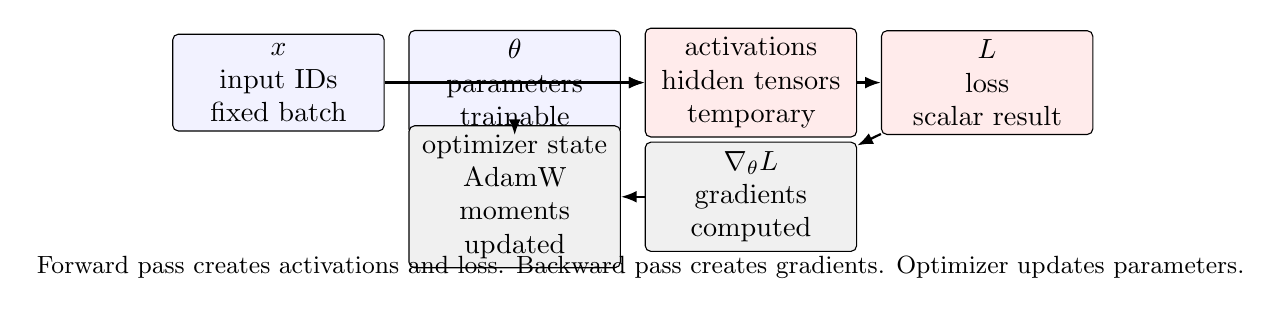
\begin{tikzpicture}[
  box/.style={draw, rounded corners=2pt, minimum height=0.72cm, text width=2.45cm, align=center},
  arrow/.style={-{Latex[length=2mm]}, thick},
  lab/.style={font=\small, align=center}
]
\node[box, fill=blue!5] (x) at (0,0) {\(x\)\\input IDs\\fixed batch};
\node[box, fill=blue!5] (theta) at (3.0,0) {\(\theta\)\\parameters\\trainable};
\node[box, fill=red!8] (act) at (6.0,0) {activations\\hidden tensors\\temporary};
\node[box, fill=red!8] (loss) at (9.0,0) {\(L\)\\loss\\scalar result};
\node[box, fill=gray!12] (grad) at (6.0,-1.45) {\(\nabla_\theta L\)\\gradients\\computed};
\node[box, fill=gray!12] (opt) at (3.0,-1.45) {optimizer state\\AdamW moments\\updated};
\draw[arrow] (x) -- (act);
\draw[arrow] (theta) -- (act);
\draw[arrow] (act) -- (loss);
\draw[arrow] (loss) -- (grad);
\draw[arrow] (grad) -- (opt);
\draw[arrow] (opt) -- (theta);
\node[lab] at (4.6,-2.35) {Forward pass creates activations and loss. Backward pass creates gradients. Optimizer updates parameters.};
\end{tikzpicture}
\end{center}

\begin{longtable}{p{0.18\textwidth}p{0.22\textwidth}p{0.22\textwidth}p{0.24\textwidth}}
\toprule
\term{Object} & \term{TinyGPT shape} & \term{Owner} & \term{Stored in checkpoint?} \\
\midrule
Token IDs \(x\) & \shape{[B,T]} & data loader & no \\
Targets \(y\) & \shape{[B,T]} & data loader & no \\
Embeddings & \shape{[V,C]} & model & yes \\
Activations & \shape{[B,T,C]} & forward pass & usually no \\
Logits & \shape{[B,T,V]} & model output & no \\
Loss \(L\) & scalar & loss function & logged, not as weight \\
Gradients & same as parameters & autograd & no \\
Optimizer state & parameter-shaped & optimizer & yes for resume \\
\bottomrule
\end{longtable}

This is the real operational logic behind the math. The equation \(f_\theta(x)=Z\) is not just notation: \(x\) comes from the data loader, \(\theta\) lives inside the model, \(Z\) is a temporary output, and the loss turns \(Z\) into a training signal.

\section{Scalars: One Number With One Meaning}

A \term{scalar} is a single number. In TinyGPT, examples include:

\begin{itemize}
  \item one loss value, such as \(L=0.446\);
  \item one learning rate, such as \(\eta=0.001\);
  \item one logit score for one token, such as \(z_7=2.2\);
  \item one probability, such as \(p_7=0.64\).
\end{itemize}

The important habit is to attach meaning to the number. The scalar \(0.64\) is not just a number. In our running example it may mean:

\[
p_{\texttt{tokens}} = 0.64,
\]

the model's probability for token ID \(7\), \texttt{tokens}, after seeing the context \texttt{Tiny GPT models learn from}.

\begin{center}
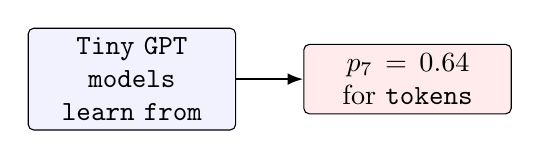
\begin{tikzpicture}[
  box/.style={draw, rounded corners=2pt, minimum height=0.65cm, text width=2.4cm, align=center},
  arrow/.style={-{Latex[length=2mm]}, thick}
]
\node[box, fill=blue!5] (context) at (0,0) {\texttt{Tiny GPT}\\\texttt{models learn from}};
\node[box, fill=red!8] (prob) at (3.5,0) {\(p_7=0.64\)\\for \texttt{tokens}};
\draw[arrow] (context) -- (prob);
\end{tikzpicture}
\end{center}

\section{Vectors: One Token Becomes A List Of Features}

A \term{vector} is an ordered list of numbers:

\[
\mathbf{v} =
\begin{bmatrix}
v_1\\v_2\\v_3\\v_4\\v_5\\v_6
\end{bmatrix}
\in \mathbb{R}^{6}.
\]

In TinyGPT, the token \texttt{Tiny} has token ID \(2\). The embedding table maps ID \(2\) to a vector of length \(C=6\):

\[
E_{\text{tok}}[2] =
\begin{bmatrix}
0.12\\
-0.04\\
0.31\\
0.08\\
-0.17\\
0.22
\end{bmatrix}.
\]

These numbers are examples, not fixed facts. At initialization they are random. During training, they change.

\begin{center}
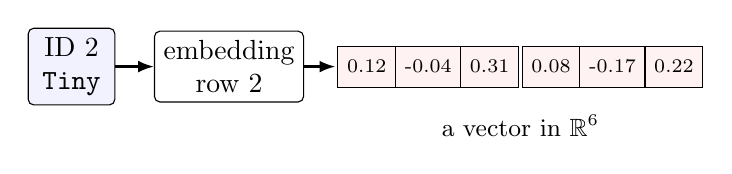
\begin{tikzpicture}[
  cell/.style={draw, minimum width=0.72cm, minimum height=0.52cm, align=center},
  box/.style={draw, rounded corners=2pt, minimum width=1.1cm, minimum height=0.65cm, align=center},
  arrow/.style={-{Latex[length=2mm]}, thick}
]
\node[box, fill=blue!5] (id) at (0,0) {ID 2\\\texttt{Tiny}};
\node[box] (row) at (2.0,0) {embedding\\row 2};
\foreach \i/\v in {0/0.12,1/-0.04,2/0.31,3/0.08,4/-0.17,5/0.22} {
  \node[cell, fill=red!5] at (3.75+\i*0.78,0) {\scriptsize \v};
}
\draw[arrow] (id) -- (row);
\draw[arrow] (row) -- (3.35,0);
\node[font=\small] at (5.7,-0.75) {a vector in \(\mathbb{R}^{6}\)};
\end{tikzpicture}
\end{center}

\term{Code logic}: an embedding lookup is an index operation.

\begin{lstlisting}[language=Python]
embedding_table = torch.randn(vocab_size, n_embd)  # [V, C]
tiny_vector = embedding_table[2]                   # [C]
\end{lstlisting}

\term{Why it works}: token IDs are discrete symbols. Vectors are numerical objects that can be added, multiplied, compared, and updated by gradient descent.

\section{Matrices: Tables That Transform Vectors}

A \term{matrix} is a rectangular array of numbers:

\[
W \in \mathbb{R}^{C \times V}.
\]

In TinyGPT, the language-model head maps a hidden vector of length \(C=6\) to vocabulary logits of length \(V=9\):

\[
\mathbf{z} = \mathbf{h} W_{\text{out}} + \mathbf{b}.
\]

The shapes are:

\[
\mathbf{h} \in \mathbb{R}^{1 \times 6},
\qquad
W_{\text{out}} \in \mathbb{R}^{6 \times 9},
\qquad
\mathbf{z} \in \mathbb{R}^{1 \times 9}.
\]

\begin{center}
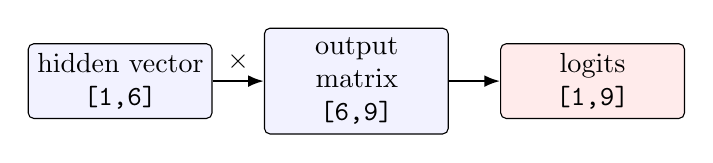
\begin{tikzpicture}[
  box/.style={draw, rounded corners=2pt, minimum height=0.75cm, text width=2.1cm, align=center},
  arrow/.style={-{Latex[length=2mm]}, thick}
]
\node[box, fill=blue!5] (h) at (0,0) {hidden vector\\\shape{[1,6]}};
\node[box, fill=blue!5] (w) at (3.0,0) {output matrix\\\shape{[6,9]}};
\node[box, fill=red!8] (z) at (6.0,0) {logits\\\shape{[1,9]}};
\draw[arrow] (h) -- node[above] {\(\times\)} (w);
\draw[arrow] (w) -- (z);
\end{tikzpicture}
\end{center}

This is a linear layer. In PyTorch:

\begin{lstlisting}[language=Python]
lm_head = torch.nn.Linear(6, 9)
z = lm_head(h)  # h: [1, 6], z: [1, 9]
\end{lstlisting}

\section{Tensors: Batches Of Structured Numbers}

A \term{tensor} is a multidimensional array. GPT training uses tensors constantly:

\begin{lstlisting}
input ids:          [B, T]
embeddings:         [B, T, C]
attention scores:   [B, H, T, T]
logits:             [B, T, V]
targets:            [B, T]
\end{lstlisting}

For TinyGPT:

\[
x \in \mathbb{Z}^{2 \times 4},
\qquad
X \in \mathbb{R}^{2 \times 4 \times 6},
\qquad
Z \in \mathbb{R}^{2 \times 4 \times 9}.
\]

\begin{center}
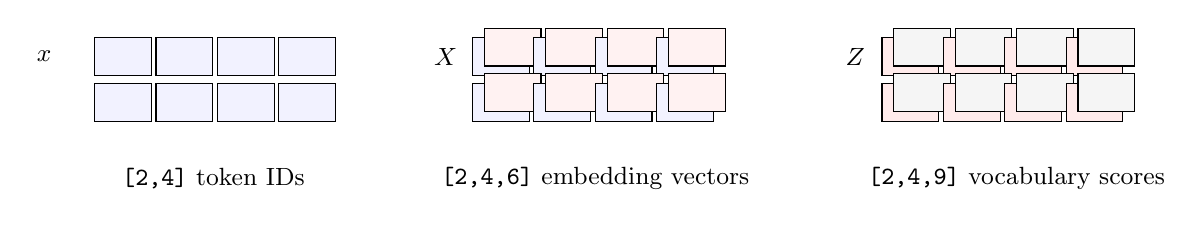
\begin{tikzpicture}[
  cell/.style={draw, minimum width=0.72cm, minimum height=0.48cm, align=center},
  lab/.style={font=\small}
]
\node[lab] at (-1.0,0) {\(x\)};
\foreach \r in {0,1} {
  \foreach \c in {0,1,2,3} {
    \node[cell, fill=blue!5] at (\c*0.78,-\r*0.58) {};
  }
}
\node[lab] at (1.15,-1.55) {\shape{[2,4]} token IDs};
\node[lab] at (4.1,0) {\(X\)};
\foreach \r in {0,1} {
  \foreach \c in {0,1,2,3} {
    \node[cell, fill=blue!5] at (4.8+\c*0.78,-\r*0.58) {};
    \node[cell, fill=red!5] at (4.95+\c*0.78,-\r*0.58+0.12) {};
  }
}
\node[lab] at (6.0,-1.55) {\shape{[2,4,6]} embedding vectors};
\node[lab] at (9.3,0) {\(Z\)};
\foreach \r in {0,1} {
  \foreach \c in {0,1,2,3} {
    \node[cell, fill=red!8] at (10.0+\c*0.78,-\r*0.58) {};
    \node[cell, fill=gray!8] at (10.15+\c*0.78,-\r*0.58+0.12) {};
  }
}
\node[lab] at (11.35,-1.55) {\shape{[2,4,9]} vocabulary scores};
\end{tikzpicture}
\end{center}

\term{Why tensors matter}: one training step should process many examples and many positions efficiently. Tensors let the code ask the GPU to perform many operations at once.

\section{Visual Tensor Geometry}

Students often understand tensors faster when they stop imagining them as mysterious objects and start seeing them as stacked tables. A tensor is an array with axes. Each axis has a meaning.

\subsection{A Rank-2 Tensor: Token IDs}

The input token tensor has shape \shape{[B,T]}. For TinyGPT, \shape{[2,4]} means two rows and four columns:

\begin{center}
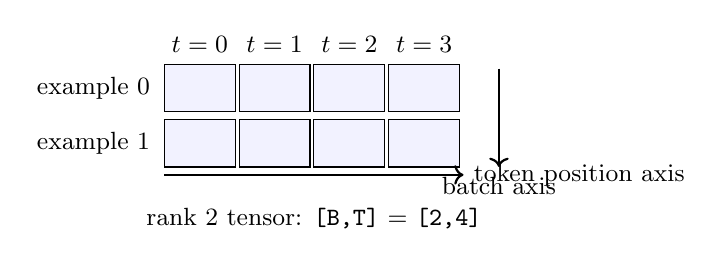
\begin{tikzpicture}[
  cell/.style={draw, minimum width=0.9cm, minimum height=0.6cm, align=center},
  lab/.style={font=\small}
]
\foreach \r/\name in {0/example 0,1/example 1} {
  \node[lab, align=right] at (-1.35,-\r*0.7) {\name};
}
\foreach \c in {0,1,2,3} {
  \node[lab] at (\c*0.95,0.55) {\(t=\c\)};
}
\foreach \r/\vals in {0/{2,3,4,5},1/{0,1,2,3}} {
  \foreach \c in {0,1,2,3} {
    \node[cell, fill=blue!5] at (\c*0.95,-\r*0.7) {};
  }
}
\node[lab] at (1.45,-1.65) {rank 2 tensor: \shape{[B,T]} = \shape{[2,4]}};
\draw[->, thick] (-0.45,-1.1) -- (3.35,-1.1) node[right] {\small token position axis};
\draw[->, thick] (3.8,0.25) -- (3.8,-1.0) node[below] {\small batch axis};
\end{tikzpicture}
\end{center}

Each cell is one integer token ID. This tensor is not yet a language representation; it is an index grid.

\subsection{A Rank-3 Tensor: Embeddings}

After embedding lookup, every token ID becomes a vector of length \(C=6\). The shape becomes \shape{[B,T,C]} = \shape{[2,4,6]}. You can visualize this as a small box: batch axis, position axis, and channel axis.

\begin{center}
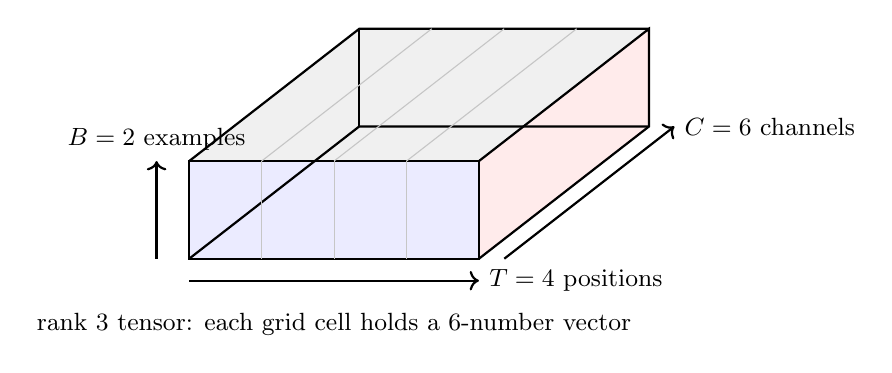
\begin{tikzpicture}[
  x={(0.92cm,0cm)},
  y={(0cm,0.62cm)},
  z={(0.36cm,0.28cm)},
  lab/.style={font=\small}
]
\coordinate (O) at (0,0,0);
\coordinate (X) at (4,0,0);
\coordinate (Y) at (0,2,0);
\coordinate (Z) at (0,0,6);
\coordinate (XY) at (4,2,0);
\coordinate (XZ) at (4,0,6);
\coordinate (YZ) at (0,2,6);
\coordinate (XYZ) at (4,2,6);

\fill[blue!8] (O) -- (X) -- (XY) -- (Y) -- cycle;
\fill[red!8] (X) -- (XZ) -- (XYZ) -- (XY) -- cycle;
\fill[gray!12] (Y) -- (XY) -- (XYZ) -- (YZ) -- cycle;
\draw[thick] (O) -- (X) -- (XY) -- (Y) -- cycle;
\draw[thick] (X) -- (XZ) -- (XYZ) -- (XY);
\draw[thick] (Y) -- (YZ) -- (XYZ);
\draw[thick] (O) -- (Z) -- (XZ);
\draw[thick] (Z) -- (YZ);

\foreach \i in {1,2,3} {
  \draw[gray!45] (\i,0,0) -- (\i,2,0);
  \draw[gray!45] (\i,2,0) -- (\i,2,6);
}
\draw[->, thick] (0,-0.45,0) -- (4,-0.45,0) node[right] {\small \(T=4\) positions};
\draw[->, thick] (-0.45,0,0) -- (-0.45,2,0) node[above] {\small \(B=2\) examples};
\draw[->, thick] (4.35,0,0) -- (4.35,0,6) node[right] {\small \(C=6\) channels};
\node[lab, align=center] at (2,-1.35,0) {rank 3 tensor: each grid cell holds a 6-number vector};
\end{tikzpicture}
\end{center}

The channel axis is where learned features live. A single position, such as token \texttt{Tiny} in example 0, is one vector:

\[
X_{0,0,:}\in\mathbb{R}^{6}.
\]

The colon means ``take all entries along this axis.'' In code:

\begin{lstlisting}[language=Python]
one_vector = X[0, 0, :]  # [C] = [6]
\end{lstlisting}

\subsection{Slices: How To Read Tensor Indexing}

Tensor indexing is easier if you think of slicing a block.

\begin{center}
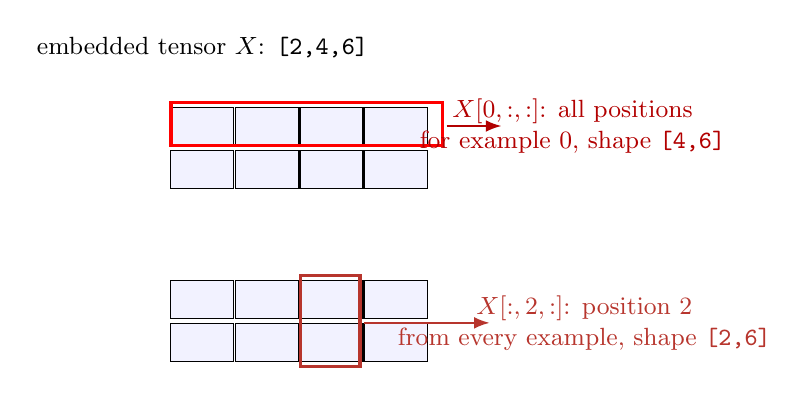
\begin{tikzpicture}[
  cell/.style={draw, minimum width=0.8cm, minimum height=0.48cm, align=center},
  lab/.style={font=\small, align=center},
  arrow/.style={-{Latex[length=2mm]}, thick}
]
\node[lab] at (0,1.0) {embedded tensor \(X\): \shape{[2,4,6]}};
\foreach \r in {0,1} {
  \foreach \c in {0,1,2,3} {
    \node[cell, fill=blue!5] at (\c*0.82,-\r*0.55) {};
  }
}
\draw[red, very thick] (-0.4,0.3) rectangle (3.05,-0.25);
\node[lab, text=red!70!black] at (4.7,0.0) {\(X[0,:,:]\): all positions\\for example 0, shape \shape{[4,6]}};
\draw[arrow, red!70!black] (3.1,0.0) -- (3.8,0.0);

\foreach \r in {0,1} {
  \foreach \c in {0,1,2,3} {
    \node[cell, fill=blue!5] at (\c*0.82,-2.2-\r*0.55) {};
  }
}
\draw[maplered, very thick] (1.25,-3.05) rectangle (2.0,-1.9);
\node[lab, text=maplered] at (4.85,-2.5) {\(X[:,2,:]\): position 2\\from every example, shape \shape{[2,6]}};
\draw[arrow, maplered] (2.05,-2.5) -- (3.65,-2.5);
\end{tikzpicture}
\end{center}

\begin{longtable}{p{0.24\textwidth}p{0.26\textwidth}p{0.34\textwidth}}
\toprule
\term{Slice} & \term{Shape} & \term{Meaning} \\
\midrule
\texttt{X[0,0,:]} & \shape{[6]} & one token vector \\
\texttt{X[0,:,:]} & \shape{[4,6]} & all positions in example 0 \\
\texttt{X[:,2,:]} & \shape{[2,6]} & position 2 from every example \\
\texttt{X[:,:,3]} & \shape{[2,4]} & channel 3 across batch and positions \\
\bottomrule
\end{longtable}

\subsection{Broadcasting: Adding Position Embeddings}

TinyGPT combines token identity and position by adding token embeddings and position embeddings:

\[
X = E_{\text{tok}}(x) + E_{\text{pos}}(0:T-1).
\]

The shapes are:

\[
\shape{[B,T,C]} + \shape{[T,C]} \rightarrow \shape{[B,T,C]}.
\]

The position matrix \shape{[T,C]} is reused for every batch row. This is called broadcasting.

\begin{center}
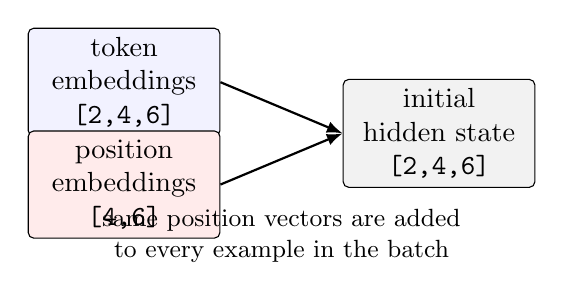
\begin{tikzpicture}[
  box/.style={draw, rounded corners=2pt, minimum height=0.75cm, text width=2.2cm, align=center},
  arrow/.style={-{Latex[length=2mm]}, thick},
  lab/.style={font=\small}
]
\node[box, fill=blue!5] (tok) at (0,0) {token embeddings\\\shape{[2,4,6]}};
\node[box, fill=red!8] (pos) at (0,-1.3) {position embeddings\\\shape{[4,6]}};
\node[box, fill=gray!10] (sum) at (4.0,-0.65) {initial hidden state\\\shape{[2,4,6]}};
\draw[arrow] (tok.east) -- (sum.west);
\draw[arrow] (pos.east) -- (sum.west);
\node[lab, align=center] at (2.0,-1.95) {same position vectors are added\\to every example in the batch};
\end{tikzpicture}
\end{center}

\term{Code logic}:

\begin{lstlisting}[language=Python]
tok = token_emb(idx)       # [B, T, C]
pos = pos_emb(positions)   # [T, C]
x = tok + pos              # [B, T, C], broadcast over B
\end{lstlisting}

\subsection{Rank-4 Tensors: Attention Scores}

Attention introduces a rank-4 tensor. If TinyGPT has \(H=2\) heads, attention scores have shape:

\[
\shape{[B,H,T,T]} = \shape{[2,2,4,4]}.
\]

The axes mean:

\begin{itemize}
  \item \(B\): which example in the batch;
  \item \(H\): which attention head;
  \item first \(T\): which position is reading;
  \item second \(T\): which position is being read.
\end{itemize}

\begin{center}
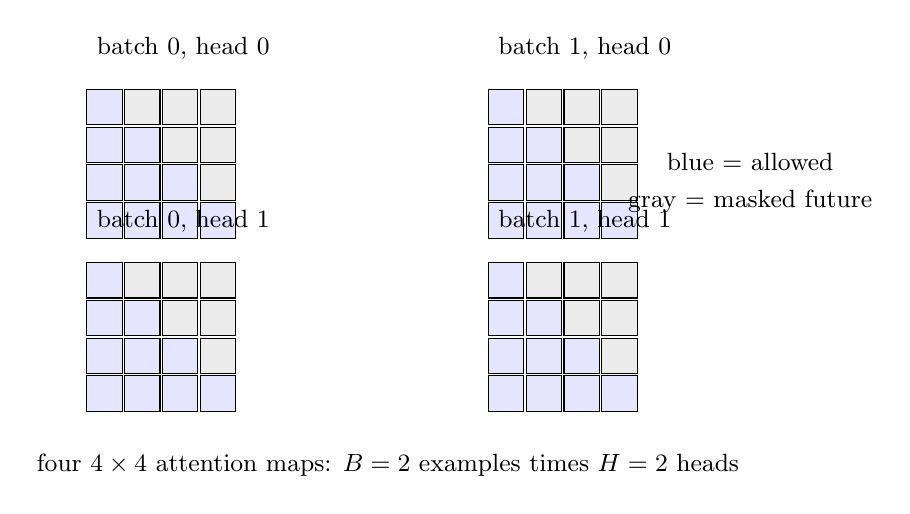
\begin{tikzpicture}[
  cell/.style={draw, minimum width=0.45cm, minimum height=0.45cm},
  lab/.style={font=\small}
]
\foreach \b/\xshift in {0/0,1/5.1} {
  \foreach \h/\yshift in {0/0,1/-2.2} {
    \node[lab] at (\xshift+1.0,\yshift+0.75) {batch \(\b\), head \(\h\)};
    \foreach \r in {0,1,2,3} {
      \foreach \c in {0,1,2,3} {
        \ifnum\c>\r
          \node[cell, fill=gray!15] at (\xshift+\c*0.48,\yshift-\r*0.48) {};
        \else
          \node[cell, fill=blue!10] at (\xshift+\c*0.48,\yshift-\r*0.48) {};
        \fi
      }
    }
  }
}
\node[lab, align=center] at (3.6,-4.55) {four \(4\times4\) attention maps: \(B=2\) examples times \(H=2\) heads};
\node[lab] at (8.2,-0.7) {blue = allowed};
\node[lab] at (8.2,-1.2) {gray = masked future};
\end{tikzpicture}
\end{center}

This diagram is the visual logic of causal attention. Each head has a table saying how much each position reads from each previous position.

\section{Preview: Context Vectors As Weighted Sums}

Attention will receive a full chapter later, but the core visual idea is useful now.
A context vector is a weighted combination of input vectors. This first arithmetic
example is \emph{unmasked} attention, not TinyGPT's causal forward pass: the second
position reads future positions too. Causal attention must instead set
\(\alpha_{23}=\alpha_{24}=0\) and renormalize the allowed weights.

Suppose TinyGPT has four token vectors:

\[
x^{(1)}=\texttt{Tiny},\quad
x^{(2)}=\texttt{GPT},\quad
x^{(3)}=\texttt{models},\quad
x^{(4)}=\texttt{learn}.
\]

To build a context vector for the second position, \(z^{(2)}\), attention computes:

\[
z^{(2)} =
\alpha_{21}x^{(1)}
+ \alpha_{22}x^{(2)}
+ \alpha_{23}x^{(3)}
+ \alpha_{24}x^{(4)}.
\]

The weights satisfy:

\[
\alpha_{21}+\alpha_{22}+\alpha_{23}+\alpha_{24}=1.
\]

\begin{center}
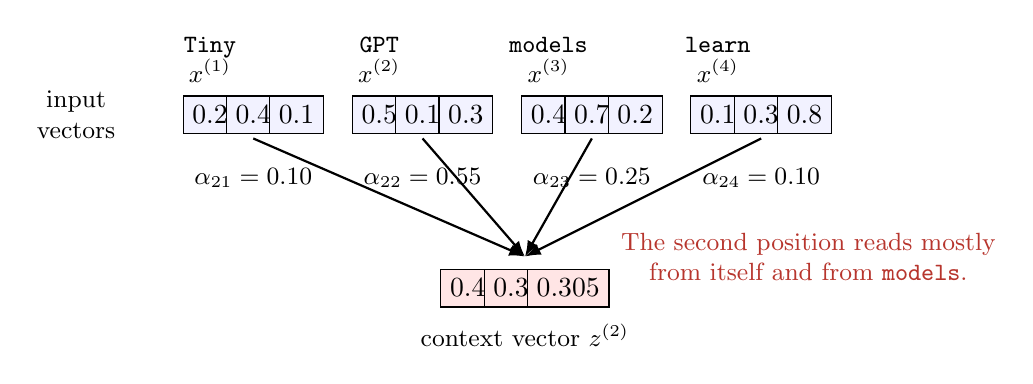
\begin{tikzpicture}[
  vec/.style={draw, minimum width=0.52cm, minimum height=0.48cm, align=center},
  word/.style={font=\small, align=center},
  arrow/.style={-{Latex[length=2mm]}, thick},
  lab/.style={font=\small, align=center}
]
\foreach \i/\tok/\a/\b/\c in {0/Tiny/0.2/0.4/0.1,1/GPT/0.5/0.1/0.3,2/models/0.4/0.7/0.2,3/learn/0.1/0.3/0.8} {
  \node[word] at (\i*2.15,1.25) {\texttt{\tok}\\\(x^{(\the\numexpr\i+1\relax)}\)};
  \node[vec, fill=blue!5] (v\i a) at (\i*2.15,0.55) {\a};
  \node[vec, fill=blue!5] (v\i b) at (\i*2.15+0.55,0.55) {\b};
  \node[vec, fill=blue!5] (v\i c) at (\i*2.15+1.10,0.55) {\c};
}
\node[lab] at (-1.7,0.55) {input\\vectors};
\foreach \i/\w in {0/0.10,1/0.55,2/0.25,3/0.10} {
  \node[lab] at (\i*2.15+0.55,-0.25) {\(\alpha_{2\the\numexpr\i+1\relax}=\w\)};
  \draw[arrow] (\i*2.15+0.55,0.25) -- (4.0,-1.25);
}
\node[vec, fill=red!10] at (3.45,-1.65) {0.405};
\node[vec, fill=red!10] at (4.0,-1.65) {0.300};
\node[vec, fill=red!10] at (4.55,-1.65) {0.305};
\node[lab] at (4.0,-2.25) {context vector \(z^{(2)}\)};
\node[lab, text=maplered] at (7.6,-1.25) {The second position reads mostly\\from itself and from \texttt{models}.};
\end{tikzpicture}
\end{center}

The numbers above are illustrative, but the mechanism is real. Attention builds a new vector by combining information from other vectors.

\section{Preview: Query, Key, Value Machinery}

The weighted-sum diagram explains what attention produces. The next diagram shows how the weights are created. Input vectors are projected into three new spaces:

\[
Q=XW_q,\qquad K=XW_k,\qquad V=XW_v.
\]

\begin{center}
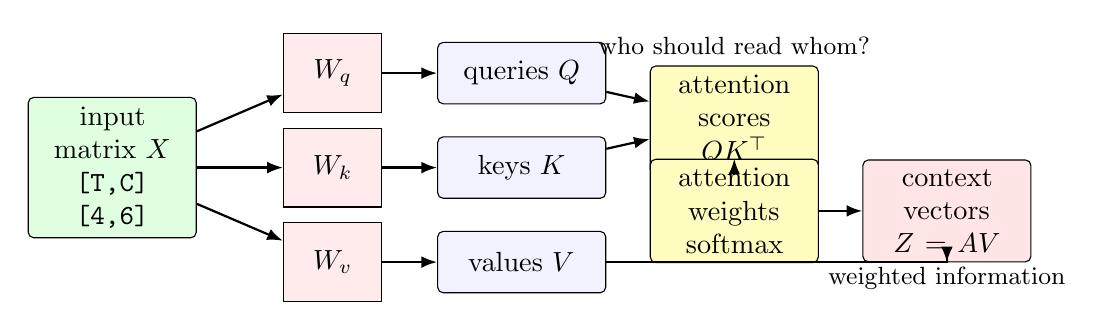
\begin{tikzpicture}[
  box/.style={draw, rounded corners=2pt, minimum height=0.78cm, text width=1.9cm, align=center},
  mat/.style={draw, minimum width=1.25cm, minimum height=1.0cm, align=center},
  arrow/.style={-{Latex[length=2mm]}, thick},
  lab/.style={font=\small, align=center}
]
\node[box, fill=green!12] (x) at (0,0) {input matrix \(X\)\\\shape{[T,C]}\\\shape{[4,6]}};
\node[mat, fill=red!8] (wq) at (2.8,1.2) {\(W_q\)};
\node[mat, fill=red!8] (wk) at (2.8,0) {\(W_k\)};
\node[mat, fill=red!8] (wv) at (2.8,-1.2) {\(W_v\)};
\node[box, fill=blue!5] (q) at (5.2,1.2) {queries \(Q\)};
\node[box, fill=blue!5] (k) at (5.2,0) {keys \(K\)};
\node[box, fill=blue!5] (v) at (5.2,-1.2) {values \(V\)};
\node[box, fill=yellow!25] (scores) at (7.9,0.6) {attention scores\\\(QK^\top\)};
\node[box, fill=yellow!25] (weights) at (7.9,-0.55) {attention weights\\softmax};
\node[box, fill=red!10] (z) at (10.6,-0.55) {context vectors\\\(Z=AV\)};
\draw[arrow] (x) -- (wq);
\draw[arrow] (x) -- (wk);
\draw[arrow] (x) -- (wv);
\draw[arrow] (wq) -- (q);
\draw[arrow] (wk) -- (k);
\draw[arrow] (wv) -- (v);
\draw[arrow] (q) -- (scores);
\draw[arrow] (k) -- (scores);
\draw[arrow] (scores) -- (weights);
\draw[arrow] (weights) -- (z);
\draw[arrow] (v) -| (z);
\node[lab] at (7.9,1.55) {who should read whom?};
\node[lab] at (10.6,-1.4) {weighted information};
\end{tikzpicture}
\end{center}

This is a preview, not the full attention lesson. The important management idea is:

\begin{itemize}
  \item \(W_q,W_k,W_v\) are trainable model parameters.
  \item \(Q,K,V\) are temporary activations created during the forward pass.
  \item attention weights are temporary probabilities over positions.
  \item context vectors are passed to later layers.
\end{itemize}

\section{Matrix Multiplication: The Workhorse}

If
\[
X \in \mathbb{R}^{B \times C},
\qquad
W \in \mathbb{R}^{C \times D},
\]
then
\[
Y = XW \in \mathbb{R}^{B \times D}.
\]

Each element is:

\[
Y_{i,j} = \sum_{k=1}^{C} X_{i,k} W_{k,j}.
\]

For TinyGPT's output head:

\[
C=6,\qquad D=V=9.
\]

One hidden vector \(\mathbf{h}\) becomes nine token scores:

\[
z_j = \sum_{k=1}^{6} h_k W_{k,j} + b_j.
\]

\begin{center}
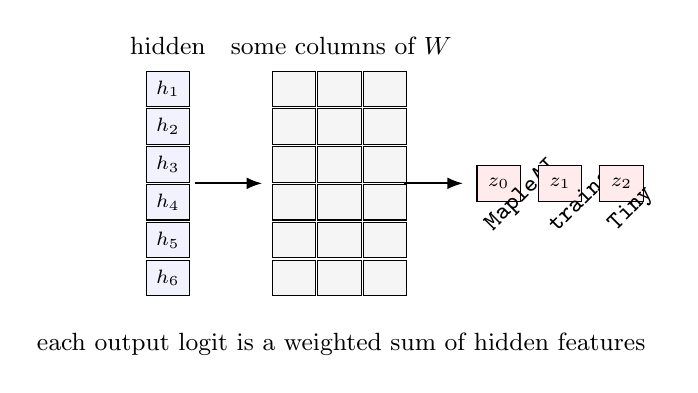
\begin{tikzpicture}[
  small/.style={draw, minimum width=0.55cm, minimum height=0.45cm, align=center},
  arrow/.style={-{Latex[length=2mm]}, thick},
  lab/.style={font=\small}
]
\foreach \i in {0,...,5} {
  \node[small, fill=blue!5] at (0,\i*-0.48) {\scriptsize \(h_{\the\numexpr\i+1\relax}\)};
}
\node[lab] at (0,0.55) {hidden};
\foreach \r in {0,...,5} {
  \foreach \c in {0,...,2} {
    \node[small, fill=gray!8] at (1.6+\c*0.58,\r*-0.48) {};
  }
}
\node[lab] at (2.2,0.55) {some columns of \(W\)};
\foreach \c/\name in {0/MapleAI,1/trains,2/Tiny} {
  \node[small, fill=red!8] at (4.2+\c*0.78,-1.2) {\scriptsize \(z_{\c}\)};
  \node[lab, rotate=45, anchor=west] at (4.0+\c*0.78,-1.85) {\texttt{\name}};
}
\draw[arrow] (0.35,-1.2) -- (1.2,-1.2);
\draw[arrow] (3.0,-1.2) -- (3.75,-1.2);
\node[lab] at (2.2,-3.25) {each output logit is a weighted sum of hidden features};
\end{tikzpicture}
\end{center}

\term{Code logic}: a linear layer is matrix multiplication plus bias.

\begin{lstlisting}[language=Python]
def linear(x, weight, bias):
    # x:      [B, C]
    # weight: [C, D]
    # bias:   [D]
    return x @ weight + bias
\end{lstlisting}

\term{Why it works}: the model learns which hidden features should increase or decrease each token's score. For example, if the hidden vector contains features suggesting the context \texttt{learn from}, the column for \texttt{tokens} should receive a high score.

\subsection{Matrix Multiplication As Rows Times Columns}

The visual rule for matrix multiplication is:

\begin{quote}
An output cell is made by matching one row from the left matrix with one column from the right matrix.
\end{quote}

For the output head, one hidden vector row multiplies each vocabulary column.

\begin{center}
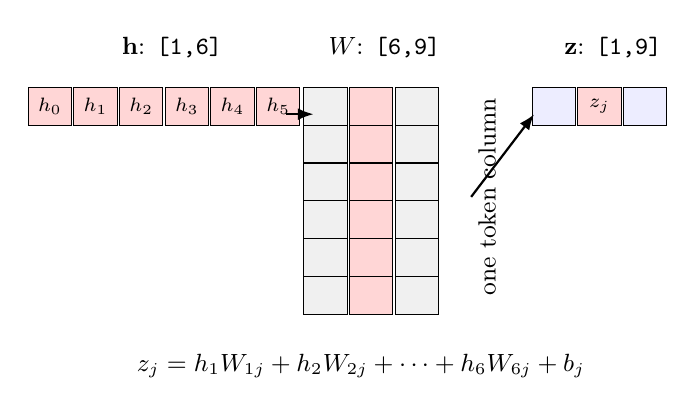
\begin{tikzpicture}[
  cell/.style={draw, minimum width=0.55cm, minimum height=0.48cm, align=center},
  hot/.style={cell, fill=red!16},
  cold/.style={cell, fill=blue!7},
  grayc/.style={cell, fill=gray!12},
  arrow/.style={-{Latex[length=2mm]}, thick},
  lab/.style={font=\small}
]
\node[lab] at (1.55,0.75) {\(\mathbf{h}\): \shape{[1,6]}};
\foreach \c in {0,1,2,3,4,5} {
  \node[hot] at (\c*0.58,0) {\scriptsize \(h_{\c}\)};
}
\node[lab] at (4.25,0.75) {\(W\): \shape{[6,9]}};
\foreach \r in {0,1,2,3,4,5} {
  \foreach \c in {0,1,2} {
    \ifnum\c=1
      \node[hot] at (3.5+\c*0.58,-\r*0.48) {};
    \else
      \node[grayc] at (3.5+\c*0.58,-\r*0.48) {};
    \fi
  }
}
\node[lab, rotate=90] at (5.55,-1.15) {one token column};
\node[lab] at (7.15,0.75) {\(\mathbf{z}\): \shape{[1,9]}};
\foreach \c in {0,1,2} {
  \ifnum\c=1
    \node[hot] at (6.4+\c*0.58,0) {\scriptsize \(z_j\)};
  \else
    \node[cold] at (6.4+\c*0.58,0) {};
  \fi
}
\draw[arrow] (3.0,-0.1) -- (3.35,-0.1);
\draw[arrow] (5.35,-1.15) -- (6.15,-0.1);
\node[lab, align=center] at (3.95,-3.3) {\(z_j=h_1W_{1j}+h_2W_{2j}+\cdots+h_6W_{6j}+b_j\)};
\end{tikzpicture}
\end{center}

If \(j=7\), this output cell is the logit for token ID \(7\), \texttt{tokens}. The model learns the column \(W_{:,7}\) so that contexts related to \texttt{learn from} produce a high \texttt{tokens} score.

\subsection{Batched Matrix Multiplication}

TinyGPT does not apply the output head to one vector only. It applies the same linear map to every position in every example:

\[
\shape{[B,T,C]} \times \shape{[C,V]}
\rightarrow
\shape{[B,T,V]}.
\]

This is like applying the same matrix to \(B\times T\) vectors.

\begin{center}
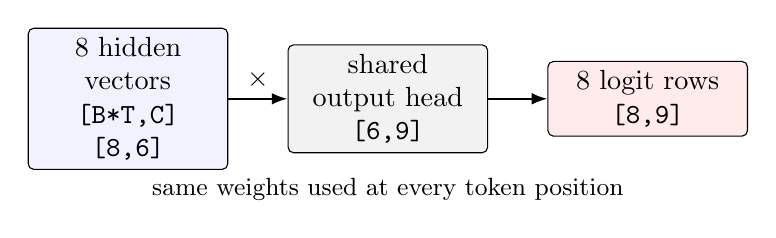
\begin{tikzpicture}[
  box/.style={draw, rounded corners=2pt, minimum height=0.75cm, text width=2.3cm, align=center},
  arrow/.style={-{Latex[length=2mm]}, thick},
  lab/.style={font=\small, align=center}
]
\node[box, fill=blue!5] (x) at (0,0) {8 hidden vectors\\\shape{[B*T,C]}\\\shape{[8,6]}};
\node[box, fill=gray!10] (w) at (3.3,0) {shared output head\\\shape{[6,9]}};
\node[box, fill=red!8] (z) at (6.6,0) {8 logit rows\\\shape{[8,9]}};
\draw[arrow] (x) -- node[above] {\(\times\)} (w);
\draw[arrow] (w) -- (z);
\node[lab] at (3.3,-1.15) {same weights used at every token position};
\end{tikzpicture}
\end{center}

Then the code may reshape back to \shape{[B,T,V]} so the result keeps its sequence structure.

\section{Dot Products: Measuring Compatibility}

The dot product of two vectors is:

\[
\mathbf{a}\cdot\mathbf{b}
= \sum_{i=1}^{d} a_i b_i.
\]

In attention, dot products compare queries and keys. For now, use a simplified story:

\begin{itemize}
  \item a query asks, ``what information do I need?''
  \item a key says, ``what information do I contain?''
  \item their dot product scores compatibility.
\end{itemize}

Suppose position \texttt{learn} is trying to predict \texttt{from}. It may strongly attend to \texttt{models} or \texttt{GPT} depending on what it has learned. The attention score is:

\[
s_{\texttt{learn},\texttt{models}}
= \frac{q_{\texttt{learn}}\cdot k_{\texttt{models}}}{\sqrt{d}}.
\]

\begin{center}
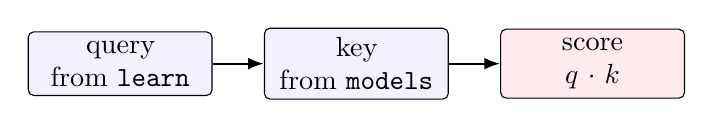
\begin{tikzpicture}[
  box/.style={draw, rounded corners=2pt, minimum height=0.7cm, text width=2.1cm, align=center},
  arrow/.style={-{Latex[length=2mm]}, thick}
]
\node[box, fill=blue!5] (q) at (0,0) {query\\from \texttt{learn}};
\node[box, fill=blue!5] (k) at (3.0,0) {key\\from \texttt{models}};
\node[box, fill=red!8] (s) at (6.0,0) {score\\\(q\cdot k\)};
\draw[arrow] (q) -- (k);
\draw[arrow] (k) -- (s);
\end{tikzpicture}
\end{center}

\section{Probability Distributions Over Tokens}

After the output head, TinyGPT has logits:

\[
\mathbf{z} =
[z_0,z_1,\ldots,z_8].
\]

These are not probabilities. They can be negative, positive, large, or small. Softmax turns them into probabilities:

\[
p_i = \operatorname{softmax}(\mathbf{z})_i =
\frac{e^{z_i}}{\sum_{j=0}^{8} e^{z_j}}.
\]

The probabilities must satisfy:

\[
p_i \geq 0,
\qquad
\sum_{i=0}^{8} p_i = 1.
\]

For the context:

\begin{quote}
\texttt{Tiny GPT models learn from}
\end{quote}

TinyGPT might produce:

\begin{longtable}{p{0.16\textwidth}p{0.22\textwidth}p{0.2\textwidth}p{0.2\textwidth}}
\toprule
\term{ID} & \term{Token} & \term{Logit} & \term{Probability} \\
\midrule
0 & \texttt{MapleAI} & -1.2 & 0.02 \\
1 & \texttt{trains} & -0.8 & 0.03 \\
2 & \texttt{Tiny} & -0.5 & 0.04 \\
3 & \texttt{GPT} & -0.4 & 0.05 \\
4 & \texttt{models} & 0.1 & 0.08 \\
5 & \texttt{learn} & 0.0 & 0.07 \\
6 & \texttt{from} & -0.7 & 0.03 \\
7 & \texttt{tokens} & 2.2 & 0.64 \\
8 & \texttt{.} & 0.4 & 0.14 \\
\bottomrule
\end{longtable}

The exact probabilities above are illustrative, but the pattern is what matters: the correct token \texttt{tokens} has the largest probability.

\begin{center}
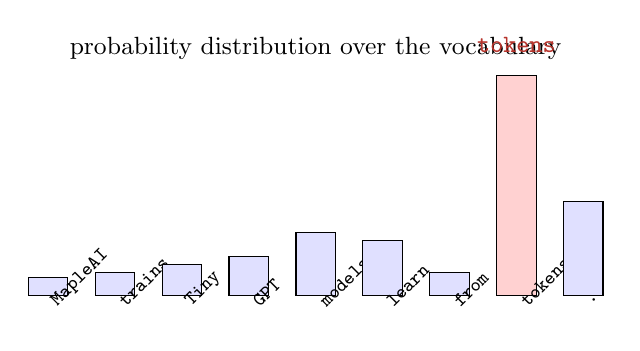
\begin{tikzpicture}[
  bar/.style={draw, fill=blue!12},
  targ/.style={draw, fill=red!18},
  lab/.style={font=\scriptsize}
]
\foreach \i/\w/\h in {0/MapleAI/0.2,1/trains/0.3,2/Tiny/0.4,3/GPT/0.5,4/models/0.8,5/learn/0.7,6/from/0.3,7/tokens/2.8,8/./1.2} {
  \ifnum\i=7
    \node[targ, anchor=south, minimum width=0.5cm, minimum height=\h cm] at (\i*0.85,0) {};
  \else
    \node[bar, anchor=south, minimum width=0.5cm, minimum height=\h cm] at (\i*0.85,0) {};
  \fi
  \node[lab, rotate=45, anchor=west] at (\i*0.85,-0.18) {\texttt{\w}};
}
\node[font=\small] at (3.4,3.15) {probability distribution over the vocabulary};
\node[font=\small, text=maplered] at (5.95,3.2) {\texttt{tokens}};
\end{tikzpicture}
\end{center}

\term{Code logic}: a numerically stable softmax subtracts the maximum logit first.

\begin{lstlisting}[language=Python]
def softmax(logits):
    shifted = logits - logits.max()
    exp_values = torch.exp(shifted)
    return exp_values / exp_values.sum()
\end{lstlisting}

\term{Why subtract the maximum}: exponentials grow quickly. Subtracting the maximum changes all logits by the same constant, so softmax probabilities stay the same, but the computation is more stable.

\section{Logarithms And Cross Entropy}

For one prediction, if the correct token ID is \(y\), the loss is:

\[
\ell = -\log p_y.
\]

In the running example:

\[
y=7,
\qquad
p_y = p_7 = 0.64.
\]

Therefore:

\[
\ell = -\log(0.64) \approx 0.446.
\]

If TinyGPT assigned \(p_7=0.05\) instead:

\[
\ell = -\log(0.05) \approx 2.996.
\]

The loss is larger because the model assigned too little probability to the correct token.

\begin{center}
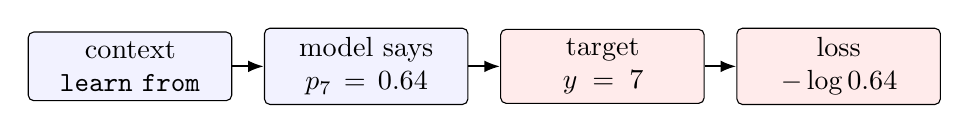
\begin{tikzpicture}[
  box/.style={draw, rounded corners=2pt, minimum height=0.68cm, text width=2.35cm, align=center},
  arrow/.style={-{Latex[length=2mm]}, thick}
]
\node[box, fill=blue!5] (context) at (0,0) {context\\\texttt{learn from}};
\node[box, fill=blue!5] (prob) at (3.0,0) {model says\\\(p_7=0.64\)};
\node[box, fill=red!8] (target) at (6.0,0) {target\\\(y=7\)};
\node[box, fill=red!8] (loss) at (9.0,0) {loss\\\(-\log 0.64\)};
\draw[arrow] (context) -- (prob);
\draw[arrow] (prob) -- (target);
\draw[arrow] (target) -- (loss);
\end{tikzpicture}
\end{center}

\term{Code logic}: cross entropy selects the probability of the correct target and takes negative log.

\begin{lstlisting}[language=Python]
def nll_loss(probs, target_id):
    return -torch.log(probs[target_id])
\end{lstlisting}

In practice, frameworks combine softmax and negative log likelihood into one stable function:

\begin{lstlisting}[language=Python]
loss = torch.nn.functional.cross_entropy(logits, targets)
\end{lstlisting}

\section{Batch Cross Entropy}

TinyGPT does not compute loss for only one prediction. With \(B=2\) and \(T=4\), it computes \(B\times T=8\) next-token predictions.

\[
L = -\frac{1}{BT}
\sum_{b=1}^{B}\sum_{t=1}^{T}
\log p_{b,t,y_{b,t}}.
\]

For our batch:

\[
x =
\begin{bmatrix}
2 & 3 & 4 & 5\\
0 & 1 & 2 & 3
\end{bmatrix},
\qquad
y =
\begin{bmatrix}
3 & 4 & 5 & 6\\
1 & 2 & 3 & 4
\end{bmatrix}.
\]

There are eight target tokens, so there are eight loss terms:

\begin{center}
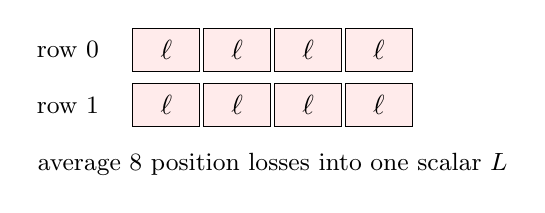
\begin{tikzpicture}[
  cell/.style={draw, minimum width=0.85cm, minimum height=0.55cm, align=center},
  lab/.style={font=\small}
]
\node[lab] at (-1.25,0) {row 0};
\node[lab] at (-1.25,-0.7) {row 1};
\foreach \r in {0,1} {
  \foreach \c in {0,1,2,3} {
    \node[cell, fill=red!8] at (\c*0.9,-\r*0.7) {\(\ell\)};
  }
}
\node[lab] at (1.35,-1.45) {average 8 position losses into one scalar \(L\)};
\end{tikzpicture}
\end{center}

\term{Code logic}: flatten the first two axes, because cross entropy sees a table of predictions.

\begin{lstlisting}[language=Python]
# logits:  [B, T, V] = [2, 4, 9]
# targets: [B, T]    = [2, 4]
loss = F.cross_entropy(
    logits.view(B * T, V),  # [8, 9]
    targets.view(B * T),    # [8]
)
\end{lstlisting}

The flattening operation can be visualized as unrolling a grid of position predictions into a list:

\begin{center}
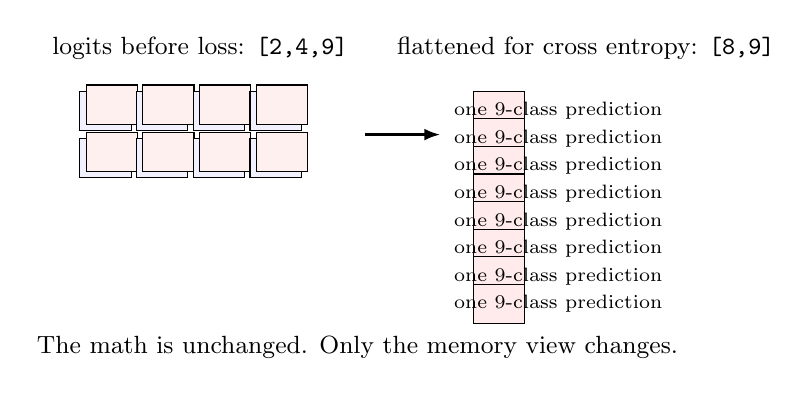
\begin{tikzpicture}[
  cell/.style={draw, minimum width=0.65cm, minimum height=0.5cm, align=center},
  arrow/.style={-{Latex[length=2mm]}, thick},
  lab/.style={font=\small}
]
\node[lab] at (1.2,0.8) {logits before loss: \shape{[2,4,9]}};
\foreach \r in {0,1} {
  \foreach \c in {0,1,2,3} {
    \node[cell, fill=blue!6] at (\c*0.72,-\r*0.6) {};
    \node[cell, fill=red!6] at (\c*0.72+0.08,-\r*0.6+0.08) {};
  }
}
\draw[arrow] (3.3,-0.3) -- (4.25,-0.3);
\node[lab] at (6.1,0.8) {flattened for cross entropy: \shape{[8,9]}};
\foreach \r in {0,1,2,3,4,5,6,7} {
  \node[cell, fill=red!8] at (5.0,-\r*0.35) {};
  \node[lab] at (5.75,-\r*0.35) {\scriptsize one 9-class prediction};
}
\node[lab, align=center] at (3.2,-3.0) {The math is unchanged. Only the memory view changes.};
\end{tikzpicture}
\end{center}

Targets flatten the same way:

\[
\shape{[2,4]} \rightarrow \shape{[8]}.
\]

Each flattened target chooses the correct class for the matching flattened logit row.

\section{Operation Gallery: Shape Changes In TinyGPT}

This gallery summarizes the visual logic of the main operations introduced so far.

\begin{longtable}{p{0.2\textwidth}p{0.26\textwidth}p{0.34\textwidth}}
\toprule
\term{Operation} & \term{Shape change} & \term{Meaning} \\
\midrule
Embedding lookup & \shape{[B,T]} \(\rightarrow\) \shape{[B,T,C]} & replace each ID with a vector \\
Position add & \shape{[B,T,C]} + \shape{[T,C]} & add order information to every batch row \\
Linear head & \shape{[B,T,C]} \(\rightarrow\) \shape{[B,T,V]} & score every vocabulary token \\
Softmax & \shape{[B,T,V]} \(\rightarrow\) \shape{[B,T,V]} & convert scores to probabilities \\
Loss flatten & \shape{[B,T,V]} \(\rightarrow\) \shape{[BT,V]} & make one row per prediction \\
Cross entropy & \shape{[BT,V]}, \shape{[BT]} \(\rightarrow\) scalar & average prediction penalty \\
\bottomrule
\end{longtable}

\begin{center}
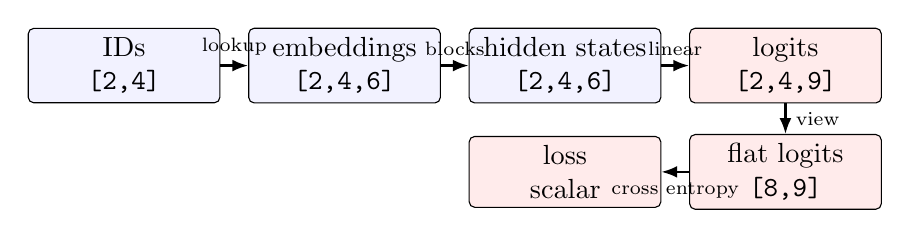
\begin{tikzpicture}[
  box/.style={draw, rounded corners=2pt, minimum height=0.7cm, text width=2.2cm, align=center},
  arrow/.style={-{Latex[length=2mm]}, thick}
]
\node[box, fill=blue!5] (a) at (0,0) {IDs\\\shape{[2,4]}};
\node[box, fill=blue!5] (b) at (2.8,0) {embeddings\\\shape{[2,4,6]}};
\node[box, fill=blue!5] (c) at (5.6,0) {hidden states\\\shape{[2,4,6]}};
\node[box, fill=red!8] (d) at (8.4,0) {logits\\\shape{[2,4,9]}};
\node[box, fill=red!8] (e) at (8.4,-1.35) {flat logits\\\shape{[8,9]}};
\node[box, fill=red!8] (f) at (5.6,-1.35) {loss\\scalar};
\draw[arrow] (a) -- node[above] {\scriptsize lookup} (b);
\draw[arrow] (b) -- node[above] {\scriptsize blocks} (c);
\draw[arrow] (c) -- node[above] {\scriptsize linear} (d);
\draw[arrow] (d) -- node[right] {\scriptsize view} (e);
\draw[arrow] (e) -- node[below] {\scriptsize cross entropy} (f);
\end{tikzpicture}
\end{center}

\section{Perplexity}

Perplexity is:

\[
\operatorname{PPL} = e^L.
\]

If validation loss is \(L=2.0\), then:

\[
\operatorname{PPL}=e^2 \approx 7.39.
\]

A rough intuition is that the model is about as uncertain as choosing among 7 or 8 plausible tokens on average. This is only an approximation, but it is useful for reading language-model logs.

\section{Functions And Parameters}

A neural network is a parameterized function:

\[
f_\theta(x)=Z.
\]

For TinyGPT:

\begin{itemize}
  \item \(x\): token IDs with shape \shape{[2,4]};
  \item \(\theta\): all model parameters;
  \item \(Z\): logits with shape \shape{[2,4,9]}.
\end{itemize}

The parameters \(\theta\) include:

\begin{lstlisting}
token embedding table
position embedding table
attention projection matrices
MLP matrices
LayerNorm weights
output head weights
\end{lstlisting}

\begin{center}
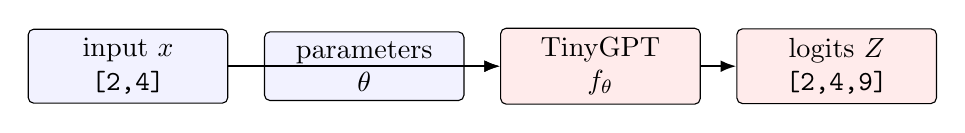
\begin{tikzpicture}[
  box/.style={draw, rounded corners=2pt, minimum height=0.7cm, text width=2.3cm, align=center},
  arrow/.style={-{Latex[length=2mm]}, thick}
]
\node[box, fill=blue!5] (x) at (0,0) {input \(x\)\\\shape{[2,4]}};
\node[box, fill=blue!5] (theta) at (3.0,0) {parameters\\\(\theta\)};
\node[box, fill=red!8] (f) at (6.0,0) {TinyGPT\\\(f_\theta\)};
\node[box, fill=red!8] (z) at (9.0,0) {logits \(Z\)\\\shape{[2,4,9]}};
\draw[arrow] (x) -- (f);
\draw[arrow] (theta) -- (f);
\draw[arrow] (f) -- (z);
\end{tikzpicture}
\end{center}

Training solves:

\[
\theta^\star = \arg\min_{\theta} L(\theta).
\]

In words: find parameter values that make the loss small.

\section{Derivatives And Gradients}

A derivative tells how a function changes when an input changes. A gradient is the multi-parameter version of this idea.

For TinyGPT, the loss \(L\) depends on many parameters. The gradient is:

\[
\nabla_\theta L =
\begin{bmatrix}
\frac{\partial L}{\partial \theta_1}\\
\frac{\partial L}{\partial \theta_2}\\
\vdots\\
\frac{\partial L}{\partial \theta_n}
\end{bmatrix}.
\]

Each entry asks:

\begin{quote}
If this parameter changes a tiny bit, how does the loss change?
\end{quote}

Gradient descent updates parameters by moving opposite the gradient:

\[
\theta_{\text{new}} =
\theta_{\text{old}} - \eta \nabla_\theta L.
\]

If a parameter change would increase loss, the update moves the other way.

\begin{center}
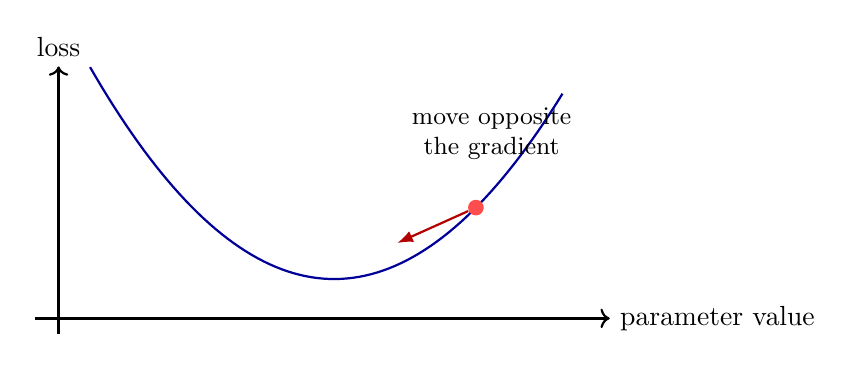
\begin{tikzpicture}[
  axis/.style={->, thick},
  arrow/.style={-{Latex[length=2mm]}, thick},
  dot/.style={circle, fill=red!70, inner sep=2pt}
]
\draw[axis] (-0.3,0) -- (7,0) node[right] {parameter value};
\draw[axis] (0,-0.2) -- (0,3.2) node[above] {loss};
\draw[thick, blue!60!black, domain=0.4:6.4, samples=80] plot (\x,{0.28*(\x-3.5)^2+0.5});
\node[dot] (p) at (5.3,{0.28*(5.3-3.5)^2+0.5}) {};
\draw[arrow, red!70!black] (p) -- ++(-1.0,-0.45);
\node[font=\small, align=center] at (5.5,2.35) {move opposite\\the gradient};
\end{tikzpicture}
\end{center}

\term{Code logic}: after \texttt{loss.backward()}, each trainable tensor has a \texttt{.grad} field.

\begin{lstlisting}[language=Python]
logits, loss = model(x, y)
loss.backward()

for name, param in model.named_parameters():
    print(name, param.shape, param.grad.shape)
\end{lstlisting}

\section{Why Backpropagation Works}

TinyGPT is a composition of functions:

\[
x
\rightarrow
\text{embeddings}
\rightarrow
\text{Transformer blocks}
\rightarrow
\text{logits}
\rightarrow
\text{loss}.
\]

Mathematically:

\[
L(x) = \ell(g_4(g_3(g_2(g_1(x))))).
\]

Backpropagation applies the chain rule through this composition. If

\[
z=g(y),\qquad y=h(x),
\]

then:

\[
\frac{dz}{dx} =
\frac{dz}{dy}
\frac{dy}{dx}.
\]

The practical meaning is:

\begin{quote}
The loss sends a learning signal backward through every operation that helped produce it.
\end{quote}

\begin{center}
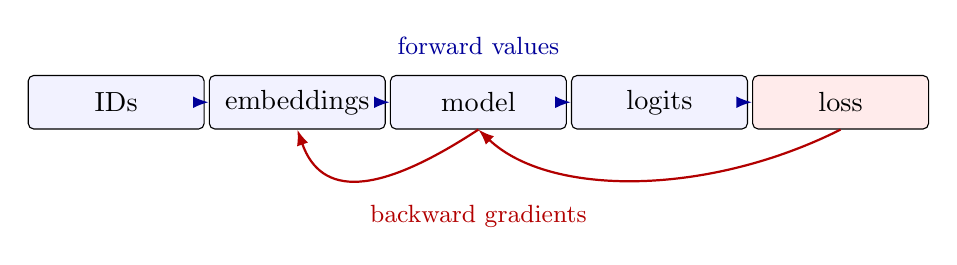
\begin{tikzpicture}[
  box/.style={draw, rounded corners=2pt, minimum height=0.68cm, text width=2.0cm, align=center},
  fwd/.style={-{Latex[length=2mm]}, thick, blue!60!black},
  bwd/.style={-{Latex[length=2mm]}, thick, red!70!black}
]
\node[box, fill=blue!5] (x) at (0,0) {IDs};
\node[box, fill=blue!5] (e) at (2.3,0) {embeddings};
\node[box, fill=blue!5] (m) at (4.6,0) {model};
\node[box, fill=blue!5] (z) at (6.9,0) {logits};
\node[box, fill=red!8] (l) at (9.2,0) {loss};
\draw[fwd] (x) -- (e);
\draw[fwd] (e) -- (m);
\draw[fwd] (m) -- (z);
\draw[fwd] (z) -- (l);
\draw[bwd] (l.south) .. controls (7.5,-1.2) and (5.5,-1.2) .. (m.south);
\draw[bwd] (m.south) .. controls (3.3,-1.2) and (2.6,-1.2) .. (e.south);
\node[font=\small, text=blue!60!black] at (4.6,0.72) {forward values};
\node[font=\small, text=red!70!black] at (4.6,-1.45) {backward gradients};
\end{tikzpicture}
\end{center}

\section{Math-To-Code Reference}

The following reference table is meant to make source code less mysterious.

\begin{longtable}{p{0.23\textwidth}p{0.24\textwidth}p{0.35\textwidth}}
\toprule
\term{Math} & \term{PyTorch idea} & \term{TinyGPT example} \\
\midrule
\(\mathbf{v}\in\mathbb{R}^{6}\) & rank-1 tensor & one token embedding \\
\(W\in\mathbb{R}^{6\times9}\) & rank-2 tensor & output head weight \\
\(X\in\mathbb{R}^{2\times4\times6}\) & rank-3 tensor & embedded batch \\
\(XW+b\) & \texttt{nn.Linear} & hidden to logits \\
\(\operatorname{softmax}(z)\) & \texttt{torch.softmax} & logits to probabilities \\
\(-\log p_y\) & cross entropy & loss for correct token \\
\(\nabla_\theta L\) & \texttt{param.grad} & parameter update signal \\
\(\theta-\eta\nabla L\) & optimizer step & improve weights \\
\bottomrule
\end{longtable}

\engineering

Before implementing any layer, write a four-line contract:

\begin{lstlisting}
input shape:
parameter shape:
output shape:
meaning of each axis:
\end{lstlisting}

For example, the output head contract is:

\begin{lstlisting}
input shape:      [B, T, C] = [2, 4, 6]
parameter shape:  [C, V]    = [6, 9]
output shape:     [B, T, V] = [2, 4, 9]
meaning:          one vocabulary score vector per position
\end{lstlisting}

Most early LLM bugs are not deep mysteries. They are shape bugs, dtype bugs, device bugs, indexing bugs, or mismatches between tokenizer and model configuration.

\labtitle{Manual Softmax And Loss}

Suppose TinyGPT has seen:

\begin{quote}
\texttt{Tiny GPT models learn from}
\end{quote}

and the next token should be \texttt{tokens}, ID \(7\). For a simplified three-token vocabulary slice, suppose the logits are:

\[
\mathbf{z} = [2.0,1.0,0.0],
\]

where index \(0\) is the correct class in the slice.

\begin{enumerate}
  \item Compute the softmax probabilities.
  \item Compute the negative log likelihood loss if the correct class is index \(0\).
  \item Compute the loss if the correct class is index \(2\).
  \item Explain which target produces the larger loss and why.
\end{enumerate}

\section{Chapter Questions}

\begin{enumerate}
  \item In TinyGPT, what does \(V=9\) mean?
  \item What is the difference between a token ID and an embedding vector?
  \item If \(B=2\), \(T=4\), and \(C=6\), what is the shape after token embedding?
  \item What shape does the output head produce if \(V=9\)?
  \item Why are logits not probabilities?
  \item What two properties must a probability distribution satisfy?
  \item Why does cross entropy use \(-\log p_y\)?
  \item Why does batch loss average over \(B\times T\) predictions?
  \item What does the gradient \(\nabla_\theta L\) tell the optimizer?
  \item Why is backpropagation connected to the chain rule?
\end{enumerate}

\section{Solutions}

\begin{enumerate}
  \item \(V=9\) means the TinyGPT vocabulary contains nine possible token IDs, \(0\) through \(8\). At each position, the model outputs nine logits.

  \item A token ID is a discrete index, such as \(2\) for \texttt{Tiny}. An embedding vector is a learned list of numbers, such as a vector in \(\mathbb{R}^{6}\), that represents the token numerically.

  \item The shape after token embedding is \shape{[2,4,6]}. There are two examples, four positions, and six embedding features per token.

  \item The output head produces \shape{[2,4,9]}. Each of the eight positions has nine vocabulary scores.

  \item Logits are raw scores. They may be negative, positive, or any real number. Probabilities must be nonnegative and sum to one, so logits need softmax first.

  \item A probability distribution must satisfy \(p_i\geq 0\) for every \(i\), and \(\sum_i p_i=1\).

  \item Cross entropy uses \(-\log p_y\) because it gives low loss when the correct token probability is high and high loss when the correct token probability is low.

  \item A batch with shape \shape{[B,T]} contains one prediction target at every position of every example. Therefore there are \(B\times T\) position losses to average.

  \item The gradient tells the optimizer how the loss changes with respect to each parameter. The optimizer uses it to adjust parameters in a direction that tends to reduce loss.

  \item Backpropagation is the chain rule applied efficiently through a computation graph. Since TinyGPT is a composition of functions, the chain rule tells how loss gradients flow backward through all operations.
\end{enumerate}

\section{Lab Solution}

For:

\[
\mathbf{z}=[2.0,1.0,0.0],
\]

compute exponentials:

\[
e^2\approx7.389,\qquad e^1\approx2.718,\qquad e^0=1.
\]

The denominator is:

\[
7.389+2.718+1=11.107.
\]

So the softmax probabilities are approximately:

\[
\left[
\frac{7.389}{11.107},
\frac{2.718}{11.107},
\frac{1}{11.107}
\right]
=
[0.665,0.245,0.090].
\]

If the correct class is index \(0\):

\[
L=-\log(0.665)\approx0.408.
\]

If the correct class is index \(2\):

\[
L=-\log(0.090)\approx2.408.
\]

The second loss is larger because the model assigned only about \(9\%\) probability to class \(2\). Cross entropy punishes the model when it gives low probability to the correct answer.

\chapter{Text, Data, And Tokenization For TinyGPT}

The first two chapters showed the TinyGPT pipeline and the math tools behind it. This chapter focuses on the beginning of the pipeline: how raw text becomes token IDs, how token IDs become training examples, and how software should store those examples for reproducible training.

The central lesson is simple:

\begin{quote}
A GPT model does not train on text. It trains on integer token sequences created by a tokenizer.
\end{quote}

\section{Chapter Goals}

By the end of this chapter, you should be able to:

\begin{itemize}
  \item explain why text must be converted into token IDs;
  \item compare character, word, and subword tokenization;
  \item trace the TinyGPT corpus into a vocabulary and token stream;
  \item explain Byte Pair Encoding with a concrete merge example;
  \item construct input-target windows from a token stream;
  \item write the code logic for \texttt{encode}, \texttt{decode}, \texttt{get\_batch}, and binary token storage;
  \item describe the data-quality checks needed before training.
\end{itemize}

\section{The TinyGPT Corpus}

We keep the same small teaching corpus:

\begin{lstlisting}
MapleAI trains Tiny GPT models .
Tiny GPT models learn from tokens .
Tokens become vectors .
Vectors flow through attention .
\end{lstlisting}

This corpus is intentionally small. It lets us inspect every token. A real training corpus may contain billions of tokens, but the logic is the same.

\begin{center}
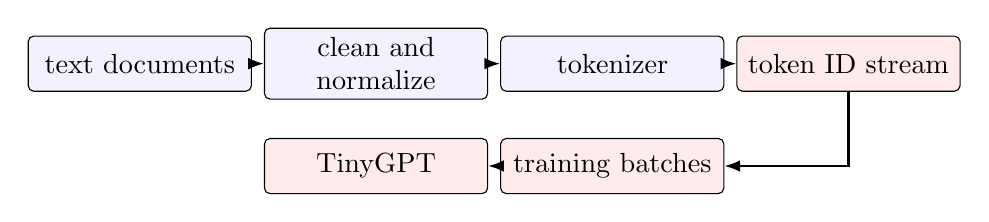
\begin{tikzpicture}[
  box/.style={draw, rounded corners=2pt, minimum height=0.7cm, text width=2.6cm, align=center},
  arrow/.style={-{Latex[length=2mm]}, thick}
]
\node[box, fill=blue!5] (docs) at (0,0) {text documents};
\node[box, fill=blue!5] (clean) at (3.0,0) {clean and normalize};
\node[box, fill=blue!5] (tok) at (6.0,0) {tokenizer};
\node[box, fill=red!8] (ids) at (9.0,0) {token ID stream};
\node[box, fill=red!8] (batches) at (6.0,-1.3) {training batches};
\node[box, fill=red!8] (model) at (3.0,-1.3) {TinyGPT};
\draw[arrow] (docs) -- (clean);
\draw[arrow] (clean) -- (tok);
\draw[arrow] (tok) -- (ids);
\draw[arrow] (ids) |- (batches);
\draw[arrow] (batches) -- (model);
\end{tikzpicture}
\end{center}

\section{Who Manages The Data?}

Data is not one thing. A training system manages a chain of artifacts. Each artifact has a different owner, format, and correctness check.

\begin{center}
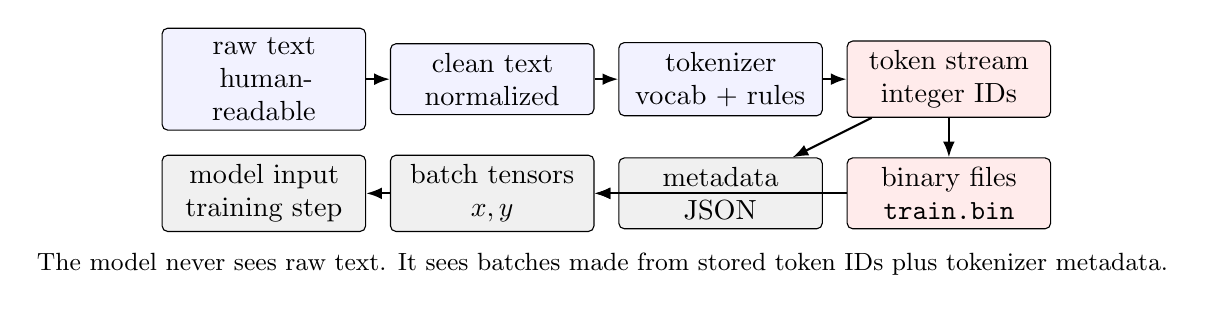
\begin{tikzpicture}[
  box/.style={draw, rounded corners=2pt, minimum height=0.72cm, text width=2.35cm, align=center},
  arrow/.style={-{Latex[length=2mm]}, thick},
  lab/.style={font=\small, align=center}
]
\node[box, fill=blue!5] (raw) at (0,0) {raw text\\human-readable};
\node[box, fill=blue!5] (clean) at (2.9,0) {clean text\\normalized};
\node[box, fill=blue!5] (tok) at (5.8,0) {tokenizer\\vocab + rules};
\node[box, fill=red!8] (ids) at (8.7,0) {token stream\\integer IDs};
\node[box, fill=red!8] (bin) at (8.7,-1.45) {binary files\\\texttt{train.bin}};
\node[box, fill=gray!12] (meta) at (5.8,-1.45) {metadata\\JSON};
\node[box, fill=gray!12] (batch) at (2.9,-1.45) {batch tensors\\\(x,y\)};
\node[box, fill=gray!12] (model) at (0,-1.45) {model input\\training step};
\draw[arrow] (raw) -- (clean);
\draw[arrow] (clean) -- (tok);
\draw[arrow] (tok) -- (ids);
\draw[arrow] (ids) -- (bin);
\draw[arrow] (ids) -- (meta);
\draw[arrow] (bin) -- (batch);
\draw[arrow] (meta) -- (batch);
\draw[arrow] (batch) -- (model);
\node[lab] at (4.3,-2.35) {The model never sees raw text. It sees batches made from stored token IDs plus tokenizer metadata.};
\end{tikzpicture}
\end{center}

\begin{longtable}{p{0.2\textwidth}p{0.25\textwidth}p{0.39\textwidth}}
\toprule
\term{Artifact} & \term{Managed by} & \term{Correctness question} \\
\midrule
Raw text & data curator & Is it allowed, useful, and safe? \\
Clean text & preprocessing script & Did normalization preserve meaning? \\
Tokenizer & tokenizer trainer/designer & Are encode/decode stable and saved? \\
Token stream & prepare script & Do IDs match the tokenizer? \\
Binary file & storage pipeline & Is dtype/count/checksum correct? \\
Batch \(x,y\) & data loader & Is the target shifted by exactly one? \\
Training sample & model/trainer & Does loss compare logits to the right targets? \\
\bottomrule
\end{longtable}

This management view prevents a common beginner mistake: thinking tokenization is a quick preprocessing detail. In reality, the tokenizer and token files are part of the model's identity.

\section{Why Text Needs Tokenization}

Computers can store text as bytes or Unicode characters, but a neural network needs tensors of numbers. The model needs a finite vocabulary:

\[
\mathcal{V} = \{0,1,\ldots,V-1\}.
\]

For TinyGPT, \(V=9\):

\begin{longtable}{p{0.24\textwidth}p{0.24\textwidth}p{0.34\textwidth}}
\toprule
\term{Token} & \term{ID} & \term{Role in sample corpus} \\
\midrule
\texttt{MapleAI} & 0 & organization token \\
\texttt{trains} & 1 & verb \\
\texttt{Tiny} & 2 & adjective/name token \\
\texttt{GPT} & 3 & model-family token \\
\texttt{models} & 4 & noun \\
\texttt{learn} & 5 & verb \\
\texttt{from} & 6 & preposition \\
\texttt{tokens} & 7 & noun \\
\texttt{.} & 8 & punctuation \\
\bottomrule
\end{longtable}

The token ID is an index. It points into the embedding table:

\[
E_{\text{tok}}\in\mathbb{R}^{V\times C}.
\]

With \(V=9\) and \(C=6\), TinyGPT uses:

\[
E_{\text{tok}}\in\mathbb{R}^{9\times6}.
\]

\begin{center}
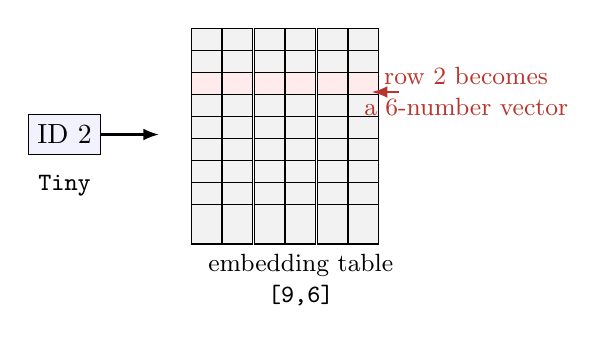
\begin{tikzpicture}[
  cell/.style={draw, minimum width=0.8cm, minimum height=0.5cm, align=center},
  lab/.style={font=\small, align=center},
  arrow/.style={-{Latex[length=2mm]}, thick}
]
\node[cell, fill=blue!5] (id) at (0,0) {ID 2};
\node[lab] at (0,-0.65) {\texttt{Tiny}};
\draw[arrow] (id) -- (1.2,0);
\foreach \r in {0,1,2,3,4,5,6,7,8} {
  \foreach \c in {0,1,2,3,4,5} {
    \ifnum\r=2
      \node[cell, fill=red!8, minimum width=0.38cm] at (1.8+\c*0.4,-\r*0.28+1.1) {};
    \else
      \node[cell, fill=gray!10, minimum width=0.38cm] at (1.8+\c*0.4,-\r*0.28+1.1) {};
    \fi
  }
}
\node[lab] at (3.0,-1.85) {embedding table\\\shape{[9,6]}};
\node[lab, text=maplered] at (5.1,0.55) {row 2 becomes\\a 6-number vector};
\draw[arrow, maplered] (4.25,0.54) -- (3.9,0.54);
\end{tikzpicture}
\end{center}

\term{Why this matters}: if the tokenizer changes, token ID \(2\) may no longer mean \texttt{Tiny}. Then the model's embedding row 2 would be interpreted incorrectly. This is why tokenizer identity is part of every serious checkpoint contract.

\section{A Token's Life Cycle}

The token \texttt{Tiny} appears simple to a reader, but the training system manages it through several representations.

\begin{center}
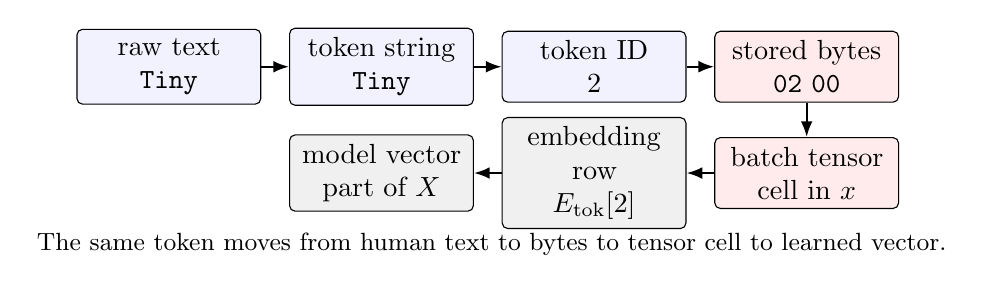
\begin{tikzpicture}[
  box/.style={draw, rounded corners=2pt, minimum height=0.72cm, text width=2.1cm, align=center},
  arrow/.style={-{Latex[length=2mm]}, thick},
  lab/.style={font=\small, align=center}
]
\node[box, fill=blue!5] (text) at (0,0) {raw text\\\texttt{Tiny}};
\node[box, fill=blue!5] (token) at (2.7,0) {token string\\\texttt{Tiny}};
\node[box, fill=blue!5] (id) at (5.4,0) {token ID\\2};
\node[box, fill=red!8] (bin) at (8.1,0) {stored bytes\\\texttt{02 00}};
\node[box, fill=red!8] (tensor) at (8.1,-1.35) {batch tensor\\cell in \(x\)};
\node[box, fill=gray!12] (embed) at (5.4,-1.35) {embedding row\\\(E_{\text{tok}}[2]\)};
\node[box, fill=gray!12] (model) at (2.7,-1.35) {model vector\\part of \(X\)};
\draw[arrow] (text) -- (token);
\draw[arrow] (token) -- (id);
\draw[arrow] (id) -- (bin);
\draw[arrow] (bin) -- (tensor);
\draw[arrow] (tensor) -- (embed);
\draw[arrow] (embed) -- (model);
\node[lab] at (4.1,-2.25) {The same token moves from human text to bytes to tensor cell to learned vector.};
\end{tikzpicture}
\end{center}

This life cycle explains why tokenizer bugs are expensive. If \texttt{Tiny} maps to the wrong ID, every later stage uses the wrong embedding row and the model learns from corrupted examples.

\section{Tokenizer Levels}

There are three useful ways to split text.

\subsection{Character-Level Tokenization}

Character tokenization splits text into characters:

\begin{quote}
\texttt{Tiny} \(\rightarrow\) \texttt{T}, \texttt{i}, \texttt{n}, \texttt{y}
\end{quote}

\begin{center}
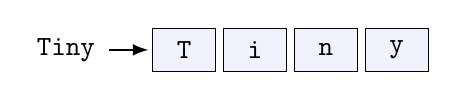
\begin{tikzpicture}[
  cell/.style={draw, minimum width=0.8cm, minimum height=0.55cm, align=center},
  arrow/.style={-{Latex[length=2mm]}, thick}
]
\node at (-1.0,0) {\texttt{Tiny}};
\draw[arrow] (-0.45,0) -- (0.05,0);
\foreach \i/\ch in {0/T,1/i,2/n,3/y} {
  \node[cell, fill=blue!5] at (\i*0.9+0.5,0) {\texttt{\ch}};
}
\end{tikzpicture}
\end{center}

\term{Strength}: very simple and handles unseen words.  
\term{Weakness}: sequences become long, so attention becomes expensive.

\subsection{Word-Level Tokenization}

Word tokenization splits text into words and punctuation:

\begin{quote}
\texttt{Tiny GPT models .} \(\rightarrow\)
\texttt{Tiny}, \texttt{GPT}, \texttt{models}, \texttt{.}
\end{quote}

This is the easiest tokenizer for our first chapters. Its weakness is that rare or unseen words are hard to handle. If the vocabulary does not contain \texttt{Transformer}, what ID should it receive?

\subsection{Subword Tokenization}

Subword tokenization splits rare words into smaller known pieces:

\begin{quote}
\texttt{tokenization} \(\rightarrow\) \texttt{token}, \texttt{ization}
\end{quote}

or, depending on the learned tokenizer:

\begin{quote}
\texttt{tokenization} \(\rightarrow\) \texttt{tok}, \texttt{en}, \texttt{ization}
\end{quote}

Subword tokenization is the common practical choice for modern LLMs because it balances sequence length and open-vocabulary behavior.

\begin{longtable}{p{0.22\textwidth}p{0.28\textwidth}p{0.32\textwidth}}
\toprule
\term{Level} & \term{Good for} & \term{Tradeoff} \\
\midrule
Character & simple demos, robustness & long sequences \\
Word & intuition, small controlled corpora & unknown words \\
Subword & practical LLM training & tokenizer training complexity \\
\bottomrule
\end{longtable}

\section{Byte Pair Encoding By Example}

Byte Pair Encoding, or BPE, learns subword tokens by repeatedly merging frequent adjacent pairs. We will use a tiny visual example.

Suppose the corpus has these word pieces:

\begin{lstlisting}
l o w
l o w
l o w e r
n e w
w i d e r
\end{lstlisting}

The pair \texttt{l o} appears often, so BPE may merge it:

\begin{center}
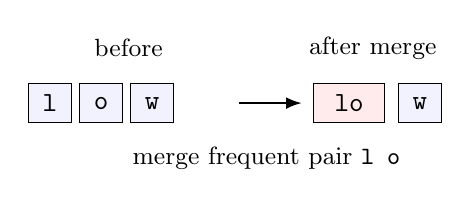
\begin{tikzpicture}[
  cell/.style={draw, minimum width=0.55cm, minimum height=0.5cm, align=center},
  arrow/.style={-{Latex[length=2mm]}, thick},
  lab/.style={font=\small, align=center}
]
\node[lab] at (1.0,0.7) {before};
\foreach \i/\ch in {0/l,1/o,2/w} {
  \node[cell, fill=blue!5] at (\i*0.65,0) {\texttt{\ch}};
}
\draw[arrow] (2.4,0) -- (3.2,0);
\node[lab] at (4.1,0.7) {after merge};
\node[cell, fill=red!8, minimum width=0.9cm] at (3.8,0) {\texttt{lo}};
\node[cell, fill=blue!5] at (4.7,0) {\texttt{w}};
\node[lab] at (2.75,-0.7) {merge frequent pair \texttt{l o}};
\end{tikzpicture}
\end{center}

Later, \texttt{lo} and \texttt{w} may merge into \texttt{low}. BPE gradually builds a vocabulary of useful pieces.

\begin{lstlisting}
start:    l o w
merge 1:  lo w
merge 2:  low
\end{lstlisting}

\term{Why BPE works}: common sequences become short tokens, while rare words can still be represented as smaller pieces. This keeps the vocabulary finite without making all sequences character-level long.

\section{Tokenizer Source Code Logic}

For TinyGPT, a word-level tokenizer is enough. A minimal implementation has four responsibilities:

\begin{enumerate}
  \item normalize text;
  \item split text into tokens;
  \item map tokens to IDs;
  \item map IDs back to tokens.
\end{enumerate}

\subsection{Normalize And Split}

\begin{lstlisting}[language=Python]
def normalize(text):
    text = text.replace(".", " .")
    text = " ".join(text.split())
    return text

def split_tokens(text):
    return normalize(text).split()
\end{lstlisting}

\term{Why this exists}: punctuation must be handled consistently. If one line contains \texttt{tokens.} and another contains \texttt{tokens .}, a word tokenizer may treat them differently unless we normalize.

\subsection{Build Vocabulary}

\begin{lstlisting}[language=Python]
def build_vocab(texts):
    tokens = []
    for text in texts:
        tokens.extend(split_tokens(text))
    unique = sorted(set(tokens))
    token_to_id = {tok: i for i, tok in enumerate(unique)}
    id_to_token = {i: tok for tok, i in token_to_id.items()}
    return token_to_id, id_to_token
\end{lstlisting}

For teaching, we manually keep the Chapter 1 order. In a real tokenizer, vocabulary order must be saved exactly.

\subsection{Encode And Decode}

\begin{lstlisting}[language=Python]
def encode(text, token_to_id):
    return [token_to_id[tok] for tok in split_tokens(text)]

def decode(ids, id_to_token):
    return " ".join(id_to_token[i] for i in ids)
\end{lstlisting}

\term{Round-trip test}:

\begin{lstlisting}[language=Python]
text = "Tiny GPT models learn from tokens."
ids = encode(text, token_to_id)
decoded = decode(ids, id_to_token)
print(ids)
print(decoded)
\end{lstlisting}

Expected IDs:

\[
[2,3,4,5,6,7,8].
\]

Expected decoded text:

\begin{quote}
\texttt{Tiny GPT models learn from tokens .}
\end{quote}

The spacing before punctuation is acceptable for this toy tokenizer. A production tokenizer should define exactly how text is reconstructed.

\section{From Documents To One Token Stream}

For next-token prediction, a corpus becomes a long sequence:

\[
s=[s_1,s_2,\ldots,s_N].
\]

Using the TinyGPT corpus, a simplified stream is:

\[
[0,1,2,3,4,8,2,3,4,5,6,7,8,\ldots].
\]

\begin{center}
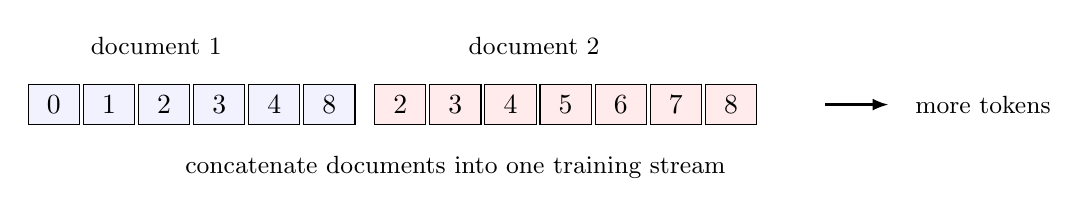
\begin{tikzpicture}[
  cell/.style={draw, minimum width=0.65cm, minimum height=0.5cm, align=center},
  lab/.style={font=\small, align=center},
  arrow/.style={-{Latex[length=2mm]}, thick}
]
\node[lab] at (1.3,0.75) {document 1};
\foreach \i/\v in {0/0,1/1,2/2,3/3,4/4,5/8} {
  \node[cell, fill=blue!5] at (\i*0.7,0) {\v};
}
\node[lab] at (6.1,0.75) {document 2};
\foreach \i/\v in {0/2,1/3,2/4,3/5,4/6,5/7,6/8} {
  \node[cell, fill=red!8] at (4.4+\i*0.7,0) {\v};
}
\draw[arrow] (9.8,0) -- (10.6,0);
\node[lab] at (11.8,0) {more tokens};
\node[lab] at (5.1,-0.8) {concatenate documents into one training stream};
\end{tikzpicture}
\end{center}

Some systems insert a special end-of-document token. TinyGPT's toy vocabulary does not include one yet, but larger training systems usually should.

\section{Train, Validation, And Test Splits}

The data must be split before training. A typical split is:

\begin{itemize}
  \item training tokens: used to update weights;
  \item validation tokens: used to monitor training decisions;
  \item test tokens: used for final reporting.
\end{itemize}

\begin{center}
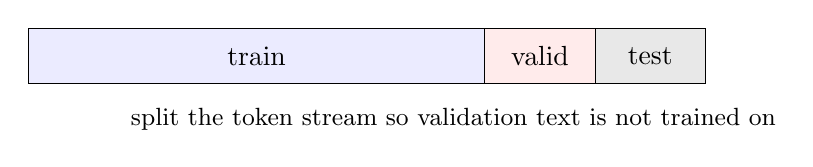
\begin{tikzpicture}[
  seg/.style={draw, minimum height=0.7cm, align=center},
  lab/.style={font=\small}
]
\node[seg, fill=blue!8, minimum width=5.8cm] at (0,0) {train};
\node[seg, fill=red!8, minimum width=1.4cm] at (3.6,0) {valid};
\node[seg, fill=gray!18, minimum width=1.4cm] at (5.0,0) {test};
\node[lab] at (2.5,-0.8) {split the token stream so validation text is not trained on};
\end{tikzpicture}
\end{center}

\term{Why this matters}: if validation examples appear in training, validation loss becomes misleadingly good. This is called leakage.

\section{Training Windows}

Given the stream:

\[
s=[2,3,4,5,6,7,8],
\]

and \(T=4\), a training window starting at index 0 uses:

\[
\text{chunk}=[2,3,4,5,6].
\]

Then:

\[
x=[2,3,4,5],
\qquad
y=[3,4,5,6].
\]

\begin{center}
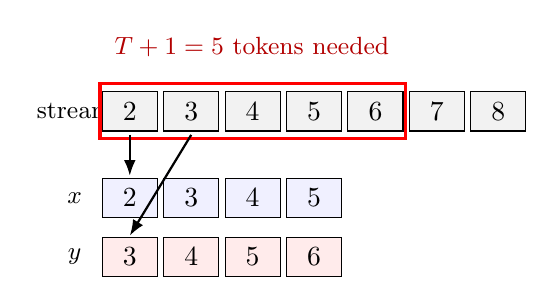
\begin{tikzpicture}[
  cell/.style={draw, minimum width=0.7cm, minimum height=0.5cm, align=center},
  lab/.style={font=\small, align=center},
  arrow/.style={-{Latex[length=2mm]}, thick}
]
\node[lab] at (-0.7,0) {stream};
\foreach \i/\v in {0/2,1/3,2/4,3/5,4/6,5/7,6/8} {
  \node[cell, fill=gray!10] at (\i*0.78,0) {\v};
}
\draw[red, very thick] (-0.38,0.35) rectangle (3.5,-0.35);
\node[lab, text=red!70!black] at (1.55,0.82) {\(T+1=5\) tokens needed};
\foreach \i/\v in {0/2,1/3,2/4,3/5} {
  \node[cell, fill=blue!6] at (\i*0.78,-1.1) {\v};
}
\node[lab] at (-0.7,-1.1) {\(x\)};
\foreach \i/\v in {0/3,1/4,2/5,3/6} {
  \node[cell, fill=red!8] at (\i*0.78,-1.85) {\v};
}
\node[lab] at (-0.7,-1.85) {\(y\)};
\draw[arrow] (0,-0.3) -- (0,-0.82);
\draw[arrow] (0.78,-0.3) -- (0,-1.58);
\end{tikzpicture}
\end{center}

This is the same shift used in Chapters 1 and 2. The dataset reader's job is to produce many such windows.

\section{Batch Construction}

A batch is several windows stacked together:

\[
X\in\mathbb{Z}^{B\times T},
\qquad
Y\in\mathbb{Z}^{B\times T}.
\]

For \(B=2\) and \(T=4\):

\[
X=
\begin{bmatrix}
2&3&4&5\\
0&1&2&3
\end{bmatrix},
\qquad
Y=
\begin{bmatrix}
3&4&5&6\\
1&2&3&4
\end{bmatrix}.
\]

\begin{center}
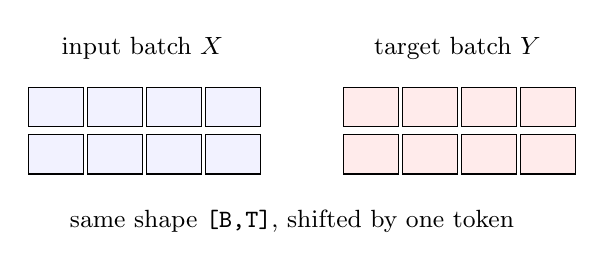
\begin{tikzpicture}[
  cell/.style={draw, minimum width=0.7cm, minimum height=0.5cm, align=center},
  lab/.style={font=\small, align=center}
]
\node[lab] at (1.1,0.75) {input batch \(X\)};
\foreach \r/\vals in {0/{2,3,4,5},1/{0,1,2,3}} {
  \foreach \c in {0,1,2,3} {
    \node[cell, fill=blue!5] at (\c*0.75,-\r*0.6) {};
  }
}
\node[lab] at (5.1,0.75) {target batch \(Y\)};
\foreach \r/\vals in {0/{3,4,5,6},1/{1,2,3,4}} {
  \foreach \c in {0,1,2,3} {
    \node[cell, fill=red!8] at (4+\c*0.75,-\r*0.6) {};
  }
}
\node[lab] at (3.0,-1.45) {same shape \shape{[B,T]}, shifted by one token};
\end{tikzpicture}
\end{center}

\section{Batch Source Code Logic}

\begin{lstlisting}[language=Python]
def get_batch(tokens, batch_size, block_size):
    # tokens is a 1D tensor or list of token IDs.
    starts = torch.randint(
        low=0,
        high=len(tokens) - block_size - 1,
        size=(batch_size,),
    )

    xs = []
    ys = []
    for i in starts:
        chunk = tokens[i : i + block_size + 1]
        xs.append(chunk[:-1])
        ys.append(chunk[1:])

    x = torch.stack(xs)  # [B, T]
    y = torch.stack(ys)  # [B, T]
    return x, y
\end{lstlisting}

\term{Function by function}:

\begin{itemize}
  \item \texttt{torch.randint}: chooses random starting positions.
  \item \texttt{chunk}: grabs \(T+1\) consecutive tokens.
  \item \texttt{chunk[:-1]}: creates the input row.
  \item \texttt{chunk[1:]}: creates the target row.
  \item \texttt{torch.stack}: turns a list of rows into a batch tensor.
\end{itemize}

\term{Why the upper bound subtracts \texttt{block\_size + 1}}: each start position must have enough future tokens to build both \(x\) and \(y\). Otherwise the target row would be too short.

\section{Binary Token Files}

Large token streams are usually stored as binary arrays. Text files are easy to inspect but slower and larger. A simple training-pack layout is:

\begin{lstlisting}
data/tokens/tinygpt/
  train.bin
  train.meta.json
  valid.bin
  valid.meta.json
\end{lstlisting}

For TinyGPT, token IDs fit in \texttt{uint16}. Larger vocabularies may require \texttt{uint32}.

\begin{center}
\begin{tikzpicture}[
  cell/.style={draw, minimum width=0.8cm, minimum height=0.55cm, align=center},
  lab/.style={font=\small, align=center}
]
\node[lab] at (-1.1,0) {tokens};
\foreach \i/\v in {0/2,1/3,2/4,3/5,4/6,5/7,6/8} {
  \node[cell, fill=blue!5] at (\i*0.85,0) {\v};
}
\node[lab] at (2.5,-0.85) {stored contiguously as binary integers};
\node[lab] at (2.5,-1.45) {\texttt{02 00 03 00 04 00 ...} for little-endian \texttt{uint16}};
\end{tikzpicture}
\end{center}

\subsection{Save And Load Code}

\begin{lstlisting}[language=Python]
import json
import numpy as np

def save_tokens(path, ids, dtype="uint16"):
    arr = np.array(ids, dtype=dtype)
    arr.tofile(path)

def load_tokens(path, dtype="uint16"):
    return np.fromfile(path, dtype=dtype)

def save_metadata(path, tokenizer_name, dtype, count, vocab_size):
    meta = {
        "tokenizer": tokenizer_name,
        "dtype": dtype,
        "count": int(count),
        "vocab_size": int(vocab_size),
        "byte_order": "little",
    }
    with open(path, "w") as f:
        json.dump(meta, f, indent=2)
\end{lstlisting}

\term{Why metadata matters}: \texttt{train.bin} alone is ambiguous. A future reader needs to know dtype, byte order, token count, tokenizer identity, and vocabulary size.

\section{Data Quality And Dataset Cards}

Data quality problems become model behavior problems. Before training, inspect:

\begin{itemize}
  \item duplicate documents;
  \item corrupted characters;
  \item broken markup;
  \item train/validation leakage;
  \item private or unsafe data;
  \item license restrictions;
  \item unexpected language mix;
  \item excessive boilerplate.
\end{itemize}

A dataset card should record:

\begin{longtable}{p{0.28\textwidth}p{0.54\textwidth}}
\toprule
\term{Field} & \term{Purpose} \\
\midrule
source & where the text came from \\
license & whether it can be used for training \\
preprocessing & normalization, filtering, deduplication \\
tokenizer & exact tokenizer name/version/hash \\
split & train, validation, test method \\
token count & number of tokens in each split \\
known risks & privacy, toxicity, quality, bias, leakage \\
checksums & reproducibility for final artifacts \\
\bottomrule
\end{longtable}

\engineering

Data code should be boring, explicit, and testable. A good data pipeline has:

\begin{lstlisting}
prepare script
tokenizer artifact
metadata JSON
binary token files
inspection tool
round-trip tests
train/valid split checks
\end{lstlisting}

The tokenizer is not a side file. It is part of the model's identity.

\labtitle{Build TinyGPT Token Data}

Use this mini-corpus:

\begin{lstlisting}
Tiny GPT models learn from tokens .
Tiny GPT models learn .
\end{lstlisting}

Use the TinyGPT vocabulary from this chapter.

\begin{enumerate}
  \item Encode each line as token IDs.
  \item Concatenate the lines into one token stream.
  \item With \(T=4\), build a window starting at position 0.
  \item Build a second window starting at position 3.
  \item State whether each window has enough tokens to form both \(x\) and \(y\).
\end{enumerate}

\section{Chapter Questions}

\begin{enumerate}
  \item Why does a GPT model need tokenization?
  \item What does \(V\) mean in the tokenizer/model contract?
  \item Why is changing the tokenizer dangerous for an existing checkpoint?
  \item What is the main weakness of character-level tokenization?
  \item What problem does subword tokenization solve?
  \item What does BPE merge during tokenizer training?
  \item Why does a training window need \(T+1\) tokens?
  \item What is train/validation leakage?
  \item Why store token streams in binary files?
  \item What metadata should accompany \texttt{train.bin}?
\end{enumerate}

\section{Solutions}

\begin{enumerate}
  \item A GPT model needs tokenization because neural networks operate on numerical tensors, not raw text. Tokenization maps text into integer IDs.

  \item \(V\) is vocabulary size. It is the number of distinct token IDs the model can read and predict. In TinyGPT, \(V=9\).

  \item Changing the tokenizer changes the meaning of token IDs. If ID \(2\) used to mean \texttt{Tiny} but later means something else, the learned embedding row 2 is misinterpreted.

  \item Character-level tokenization creates long sequences. Long sequences increase attention cost and make learning longer-range patterns harder.

  \item Subword tokenization handles rare or unseen words by splitting them into smaller known pieces while keeping common words or pieces compact.

  \item BPE merges frequent adjacent symbol pairs, such as \texttt{l} and \texttt{o} into \texttt{lo}, then possibly \texttt{lo} and \texttt{w} into \texttt{low}.

  \item A training window needs \(T+1\) tokens because \(T\) input positions require \(T\) next-token targets. The final input position needs one extra future token.

  \item Train/validation leakage happens when validation examples appear in training data. It makes validation metrics too optimistic.

  \item Binary files are compact and fast to read. They let training code stream large token arrays efficiently.

  \item Metadata should include tokenizer identity, dtype, token count, vocabulary size, byte order, split name, and ideally checksum/source information.
\end{enumerate}

\section{Lab Solution}

The first line:

\begin{quote}
\texttt{Tiny GPT models learn from tokens .}
\end{quote}

encodes as:

\[
[2,3,4,5,6,7,8].
\]

The second line:

\begin{quote}
\texttt{Tiny GPT models learn .}
\end{quote}

encodes as:

\[
[2,3,4,5,8].
\]

Concatenated stream:

\[
s=[2,3,4,5,6,7,8,2,3,4,5,8].
\]

With \(T=4\), a window starting at position 0 uses:

\[
\text{chunk}=[2,3,4,5,6].
\]

So:

\[
x=[2,3,4,5],
\qquad
y=[3,4,5,6].
\]

A window starting at position 3 uses:

\[
\text{chunk}=[5,6,7,8,2].
\]

So:

\[
x=[5,6,7,8],
\qquad
y=[6,7,8,2].
\]

Both windows have enough tokens because each has \(T+1=5\) tokens available.


\part{Model Mechanics}
\chapter{Tensors And The PyTorch Reference Path}

PyTorch is the first implementation path in this book because it makes the hidden machinery visible enough for students. A production training system may later use Rust/Candle, C/CUDA, or specialized kernels, but PyTorch is the best place to learn the mathematical contract of a GPT model.

This chapter is not a general PyTorch manual. It is a TinyGPT engineering chapter. Every tensor, module, gradient, and normalization operation is explained through the running GPT example.

\section{Chapter Goals}

By the end of this chapter, you should be able to:

\begin{itemize}
  \item read tensor shapes as part of the program's meaning;
  \item explain how token IDs become embedding tensors in PyTorch;
  \item trace a TinyGPT forward pass through modules and functions;
  \item explain \texttt{nn.Module}, parameters, buffers, devices, and dtypes;
  \item compute layer normalization for one token vector by hand;
  \item connect \texttt{loss.backward()} to the chain rule and parameter gradients;
  \item use shape assertions and tiny experiments to debug a GPT implementation.
\end{itemize}

\section{Why The PyTorch Path Is Called A Reference Path}

The project should not call the PyTorch implementation simply ``gpt21,'' because \texttt{gpt21} describes a model family and learning pack, not one backend. A clearer structure is:

\begin{lstlisting}
llm-train/
  mapletrain/
    torch_reference/      # readable educational implementation
    candle_backend/       # Rust/Candle implementation
    cuda_backend/         # C/CUDA or llm.c-inspired implementation
  scripts/
    train_torch.py
    train_candle.py
    inspect_tokens.py
\end{lstlisting}

The phrase \term{reference path} has a specific meaning:

\begin{itemize}
  \item it is the implementation students read first;
  \item it should prefer clarity over maximum speed;
  \item it defines expected tensor shapes and loss behavior;
  \item other backends should be compared against it.
\end{itemize}

\begin{center}
\begin{tikzpicture}[
  box/.style={draw, rounded corners=2pt, minimum height=0.72cm, text width=2.55cm, align=center},
  arrow/.style={-{Latex[length=2mm]}, thick},
  note/.style={font=\small, align=center}
]
\node[box, fill=blue!5] (data) at (0,0) {shared token data\\\shape{train.bin}};
\node[box, fill=red!8] (torch) at (3.2,1.0) {PyTorch\\reference path};
\node[box, fill=green!10] (candle) at (3.2,0) {Rust/Candle\\systems path};
\node[box, fill=gray!12] (cuda) at (3.2,-1.0) {C/CUDA\\kernel path};
\node[box, fill=yellow!18] (compare) at (6.5,0) {compare\\loss, samples,\\throughput};
\draw[arrow] (data) -- (torch);
\draw[arrow] (data) -- (candle);
\draw[arrow] (data) -- (cuda);
\draw[arrow] (torch) -- (compare);
\draw[arrow] (candle) -- (compare);
\draw[arrow] (cuda) -- (compare);
\node[note] at (3.15,-2.0) {The same math should survive across different engineering backends.};
\end{tikzpicture}
\end{center}

\section{The TinyGPT Tensor Contract}

The central rule is simple:

\begin{quote}
Every tensor shape is a promise about what the numbers mean.
\end{quote}

For TinyGPT, we continue to use:

\[
B=2,\qquad T=4,\qquad C=6,\qquad V=9.
\]

\begin{longtable}{p{0.22\textwidth}p{0.20\textwidth}p{0.44\textwidth}}
\toprule
\term{Tensor} & \term{Shape} & \term{Meaning} \\
\midrule
\texttt{x} & \shape{[B,T]} & token IDs used as model input \\
\texttt{y} & \shape{[B,T]} & next-token target IDs \\
\texttt{tok\_emb(x)} & \shape{[B,T,C]} & token embedding vector at each position \\
\texttt{pos\_emb(pos)} & \shape{[T,C]} & learned vector for each position \\
\texttt{h} & \shape{[B,T,C]} & hidden activations inside the model \\
\texttt{att} & \shape{[B,H,T,T]} & attention scores or probabilities \\
\texttt{logits} & \shape{[B,T,V]} & one vocabulary score per position \\
\texttt{loss} & scalar & average training error for the batch \\
\bottomrule
\end{longtable}

\begin{center}
\begin{tikzpicture}[
  box/.style={draw, rounded corners=2pt, minimum height=0.7cm, text width=2.35cm, align=center},
  arrow/.style={-{Latex[length=2mm]}, thick},
  small/.style={font=\small, align=center}
]
\node[box, fill=blue!5] (ids) at (0,0) {token IDs\\\shape{[2,4]}};
\node[box, fill=blue!5] (emb) at (2.9,0) {embeddings\\\shape{[2,4,6]}};
\node[box, fill=red!8] (block) at (5.8,0) {GPT blocks\\\shape{[2,4,6]}};
\node[box, fill=red!8] (logits) at (8.7,0) {logits\\\shape{[2,4,9]}};
\node[box, fill=yellow!18] (loss) at (11.3,0) {loss\\scalar};
\draw[arrow] (ids) -- node[small, above] {lookup} (emb);
\draw[arrow] (emb) -- node[small, above] {mix context} (block);
\draw[arrow] (block) -- node[small, above] {linear head} (logits);
\draw[arrow] (logits) -- node[small, above] {cross entropy} (loss);
\end{tikzpicture}
\end{center}

\section{Tensor Shapes As Types}

In ordinary programming, a type might say ``integer'' or ``string.'' In GPT programming, a shape often carries just as much meaning.

\[
x \in \mathbb{Z}^{B \times T}
\]

means that \(x\) is a two-dimensional tensor of token IDs. The two axes mean:

\begin{itemize}
  \item axis 0: which training example in the batch;
  \item axis 1: which token position in the context window.
\end{itemize}

After embedding lookup:

\[
X = E_{\text{tok}}[x] \in \mathbb{R}^{B \times T \times C}.
\]

Now the axes mean:

\begin{itemize}
  \item axis 0: batch example;
  \item axis 1: token position;
  \item axis 2: learned feature dimension.
\end{itemize}

\begin{center}
\begin{tikzpicture}[
  cell/.style={draw, minimum width=0.65cm, minimum height=0.45cm, align=center},
  box/.style={draw, rounded corners=2pt, minimum height=0.65cm, text width=1.85cm, align=center},
  arrow/.style={-{Latex[length=2mm]}, thick}
]
\node[box, fill=blue!5] (ids) at (0,0) {\shape{[B,T]}\\IDs};
\foreach \r in {0,1} {
  \foreach \c in {0,1,2,3} {
    \node[cell, fill=blue!5] at (2+\c*0.65,-\r*0.45) {\scriptsize};
  }
}
\node[font=\small] at (2.95,0.45) {\(x\)};
\node[box, fill=red!8] (emb) at (5.6,-0.23) {\shape{[B,T,C]}\\vectors};
\foreach \r in {0,1} {
  \foreach \c in {0,1,2,3} {
    \draw[fill=red!6] (7+\c*0.56,-\r*0.48) -- +(0.42,0) -- +(0.54,0.16) -- +(0.12,0.16) -- cycle;
    \draw (7+\c*0.56,-\r*0.48) rectangle +(0.42,0.34);
    \draw (7.42+\c*0.56,-\r*0.48) -- +(0.12,0.16);
    \draw (7.42+\c*0.56,-\r*0.14) -- +(0.12,0.16);
    \draw (7+\c*0.56,-\r*0.14) -- +(0.12,0.16);
  }
}
\draw[arrow] (ids) -- (1.5,-0.22);
\draw[arrow] (4.85,-0.23) -- (emb);
\draw[arrow] (emb) -- (6.65,-0.23);
\node[font=\small] at (8.05,0.55) {each ID becomes a length-\(C\) feature vector};
\end{tikzpicture}
\end{center}

\term{Engineering rule}: never rely on memory alone. Write the expected shapes near the code that creates them.

\begin{lstlisting}[language=Python]
B, T, C, V = 2, 4, 6, 9
x = torch.tensor([[2, 3, 4, 5],
                  [3, 4, 5, 6]])       # [B, T]
tok_emb = nn.Embedding(V, C)
X = tok_emb(x)                          # [B, T, C]
assert X.shape == (B, T, C)
\end{lstlisting}

\section{Minimal PyTorch Objects}

The most important PyTorch objects are:

\begin{longtable}{p{0.23\textwidth}p{0.62\textwidth}}
\toprule
\term{Object} & \term{Role in TinyGPT} \\
\midrule
\texttt{torch.Tensor} & multidimensional array with shape, dtype, and device \\
\texttt{nn.Parameter} & trainable tensor owned by a module \\
\texttt{nn.Module} & object that owns layers and defines \texttt{forward} \\
\texttt{Optimizer} & updates parameters using gradients \\
\texttt{autograd} & records operations and computes derivatives \\
\bottomrule
\end{longtable}

The model is not just code. It is code plus owned tensors.

\begin{center}
\begin{tikzpicture}[
  box/.style={draw, rounded corners=2pt, minimum height=0.65cm, text width=2.65cm, align=center},
  arrow/.style={-{Latex[length=2mm]}, thick}
]
\node[box, fill=blue!5] (module) at (0,0) {\texttt{TinyGPT}\\\texttt{nn.Module}};
\node[box, fill=red!8] (params) at (3.2,1.0) {parameters\\embedding, linear,\\LayerNorm};
\node[box, fill=gray!12] (forward) at (3.2,0) {\texttt{forward(x,y)}\\computation};
\node[box, fill=yellow!18] (children) at (3.2,-1.0) {child modules\\blocks, attention,\\MLP};
\node[box, fill=green!10] (outputs) at (6.4,0) {logits, loss};
\draw[arrow] (module) -- (params);
\draw[arrow] (module) -- (forward);
\draw[arrow] (module) -- (children);
\draw[arrow] (params) -- (forward);
\draw[arrow] (children) -- (forward);
\draw[arrow] (forward) -- (outputs);
\end{tikzpicture}
\end{center}

\section{A Linear Layer As A Wiring Diagram}

A linear layer computes:

\[
Y = XW^\top + b.
\]

PyTorch stores \texttt{nn.Linear(in\_features, out\_features)} weights with shape:

\[
W \in \mathbb{R}^{\text{out\_features} \times \text{in\_features}}.
\]

Mathematically, for one input vector \(\mathbf{x}\in \mathbb{R}^{C}\):

\[
y_j = \sum_{i=1}^{C} W_{j,i}x_i + b_j.
\]

For TinyGPT with \(C=6\), a small hidden vector can be transformed into another six-dimensional vector:

\begin{center}
\begin{tikzpicture}[
  neuron/.style={circle, draw, minimum size=0.68cm, align=center},
  arrow/.style={-{Latex[length=1.8mm]}, thin},
  lab/.style={font=\small, align=center}
]
\foreach \i/\v in {0/0.12,1/-0.04,2/0.31,3/0.08,4/-0.17,5/0.22} {
  \node[neuron, fill=blue!5] (x\i) at (0,-\i*0.58) {\scriptsize \v};
}
\foreach \j/\v in {0/0.19,1/0.00,2/0.43,3/0.11,4/-0.08,5/0.27} {
  \node[neuron, fill=red!8] (y\j) at (4.4,-\j*0.58) {\scriptsize \v};
}
\foreach \i in {0,1,2,3,4,5} {
  \foreach \j in {0,1,2,3,4,5} {
    \draw[arrow, opacity=0.25] (x\i) -- (y\j);
  }
}
\node[lab] at (0,0.75) {input\\features};
\node[lab] at (4.4,0.75) {output\\features};
\node[lab] at (2.2,-3.9) {Each output feature is a weighted sum of all input features plus a bias.};
\end{tikzpicture}
\end{center}

\begin{lstlisting}[language=Python]
layer = nn.Linear(6, 6)
y = layer(x)          # x: [6], y: [6]
\end{lstlisting}

When the same layer receives a rank-3 tensor \shape{[B,T,C]}, PyTorch applies the same linear transformation independently to every \shape{[C]} vector:

\begin{lstlisting}[language=Python]
h = torch.randn(B, T, C)
y = layer(h)          # [B, T, C]
\end{lstlisting}

\section{Layer Normalization: Stabilizing One Token Vector}

Layer normalization is one of the most important operations inside GPT blocks. It makes each token's feature vector easier for the next sublayer to process.

For one token vector:

\[
\mathbf{x} =
\begin{bmatrix}
0.22 & 0.34 & 0.00 & 0.22 & 0.00 & 0.00
\end{bmatrix},
\]

layer normalization first computes the mean across the feature dimension:

\[
\mu = \frac{1}{C}\sum_{i=1}^{C}x_i.
\]

Then it computes the variance:

\[
\sigma^2 = \frac{1}{C}\sum_{i=1}^{C}(x_i-\mu)^2.
\]

Then it normalizes every feature:

\[
\hat{x}_i = \frac{x_i-\mu}{\sqrt{\sigma^2+\epsilon}}.
\]

Finally it learns a scale and shift:

\[
y_i = \gamma_i \hat{x}_i + \beta_i.
\]

Here \(\gamma,\beta \in \mathbb{R}^{C}\) are trainable parameters. At initialization, PyTorch usually starts with \(\gamma_i=1\) and \(\beta_i=0\).

\begin{center}
\begin{tikzpicture}[
  cell/.style={draw, circle, minimum size=0.72cm, align=center},
  box/.style={draw, rounded corners=4pt, minimum height=0.58cm, text width=5.4cm, align=center},
  arrow/.style={-{Latex[length=2mm]}, thick},
  note/.style={font=\small, align=center}
]
\foreach \i/\v in {0/0.22,1/0.34,2/0.00,3/0.22,4/0.00,5/0.00} {
  \node[cell, fill=blue!5] (a\i) at (\i*1.02,0) {\scriptsize \v};
}
\node[note, anchor=east] at (-0.45,0) {activation vector\\for one token};

\node[box, fill=yellow!18] (stats) at (2.55,1.35) {compute \(\mu=0.13\), \(\sigma^2\approx0.016\) across the six features};
\node[box, fill=gray!12] (norm) at (2.55,2.45) {subtract mean, divide by standard deviation};
\foreach \i/\v in {0/0.72,1/1.68,2/-1.04,3/0.72,4/-1.04,5/-1.04} {
  \node[cell, fill=red!8] (b\i) at (\i*1.02,3.55) {\scriptsize \v};
}
\node[note, anchor=west] at (6.4,3.55) {roughly zero mean\\and unit variance};

\foreach \i in {0,1,2,3,4,5} {
  \draw[arrow] (a\i) -- (stats);
  \draw[arrow] (norm) -- (b\i);
}
\draw[arrow] (stats) -- (norm);
\node[note] at (2.55,-0.78) {LayerNorm normalizes across features for the same token position, not across the batch.};
\end{tikzpicture}
\end{center}

This is the key visual idea: each token position carries a feature vector, and LayerNorm cleans up that vector before the next operation uses it.

\subsection{LayerNorm In A Batch}

For a full hidden tensor:

\[
h \in \mathbb{R}^{B \times T \times C},
\]

LayerNorm normalizes along the final axis \(C\). It does this separately for every pair \((b,t)\).

\begin{center}
\begin{tikzpicture}[
  cube/.style={draw, fill=blue!5},
  slice/.style={draw, fill=red!8},
  arrow/.style={-{Latex[length=2mm]}, thick},
  note/.style={font=\small, align=center}
]
\draw[cube] (0,0) rectangle (2.8,1.5);
\draw[cube] (0.35,0.35) rectangle (3.15,1.85);
\draw (0,1.5) -- (0.35,1.85);
\draw (2.8,1.5) -- (3.15,1.85);
\draw (2.8,0) -- (3.15,0.35);
\node[note] at (1.55,0.78) {\(h\)\\\shape{[B,T,C]}};

\draw[slice] (4.7,0.55) rectangle (7.0,1.05);
\foreach \i in {0,1,2,3,4,5} {
  \draw (4.7+\i*0.38,0.55) rectangle +(0.38,0.5);
}
\node[note] at (5.85,1.45) {one token vector\\\shape{[C]}};
\draw[arrow] (3.2,0.9) -- (4.55,0.8);
\node[note] at (5.85,-0.15) {mean and variance are computed here};

\node[note] at (1.55,-0.65) {choose one batch row and one time position};
\end{tikzpicture}
\end{center}

In code:

\begin{lstlisting}[language=Python]
ln = nn.LayerNorm(C)
h = torch.randn(B, T, C)
out = ln(h)          # [B, T, C]
\end{lstlisting}

The shape does not change. Only the values change.

\subsection{Why GPT Uses LayerNorm}

During training, hidden activations can drift. Some features become too large, some too small, and different layers may receive inputs on very different scales. LayerNorm helps by giving each token vector a predictable scale before attention or the MLP sees it.

Modern GPT implementations often use \term{pre-normalization}:

\[
h \leftarrow h + \operatorname{Attention}(\operatorname{LayerNorm}(h)),
\]

\[
h \leftarrow h + \operatorname{MLP}(\operatorname{LayerNorm}(h)).
\]

\begin{center}
\begin{tikzpicture}[
  box/.style={draw, rounded corners=2pt, minimum height=0.62cm, text width=1.95cm, align=center},
  arrow/.style={-{Latex[length=2mm]}, thick},
  plus/.style={circle, draw, minimum size=0.55cm, align=center}
]
\node[box, fill=blue!5] (h0) at (0,0) {\(h\)};
\node[box, fill=yellow!18] (ln1) at (2.0,0) {LayerNorm};
\node[box, fill=red!8] (attn) at (4.0,0) {Attention};
\node[plus] (add1) at (6.0,0) {\(+\)};
\node[box, fill=blue!5] (h1) at (7.5,0) {\(h'\)};
\node[box, fill=yellow!18] (ln2) at (9.5,0) {LayerNorm};
\node[box, fill=red!8] (mlp) at (11.5,0) {MLP};
\node[plus] (add2) at (13.5,0) {\(+\)};
\node[box, fill=blue!5] (h2) at (15.0,0) {output};
\draw[arrow] (h0) -- (ln1);
\draw[arrow] (ln1) -- (attn);
\draw[arrow] (attn) -- (add1);
\draw[arrow] (add1) -- (h1);
\draw[arrow] (h0) .. controls (2,-1.2) and (4,-1.2) .. (add1);
\draw[arrow] (h1) -- (ln2);
\draw[arrow] (ln2) -- (mlp);
\draw[arrow] (mlp) -- (add2);
\draw[arrow] (add2) -- (h2);
\draw[arrow] (h1) .. controls (9.5,-1.2) and (11.5,-1.2) .. (add2);
\end{tikzpicture}
\end{center}

The residual paths carry the original information forward. The LayerNorm paths prepare stable inputs for the trainable sublayers.

\section{LayerNorm Source Code Logic}

A minimal educational LayerNorm implementation is:

\begin{lstlisting}[language=Python]
class TinyLayerNorm(nn.Module):
    def __init__(self, n_embd, eps=1e-5):
        super().__init__()
        self.gamma = nn.Parameter(torch.ones(n_embd))
        self.beta = nn.Parameter(torch.zeros(n_embd))
        self.eps = eps

    def forward(self, x):
        # x: [B, T, C]
        mean = x.mean(dim=-1, keepdim=True)              # [B, T, 1]
        var = ((x - mean) ** 2).mean(dim=-1, keepdim=True)
        x_hat = (x - mean) / torch.sqrt(var + self.eps)  # [B, T, C]
        return self.gamma * x_hat + self.beta            # [B, T, C]
\end{lstlisting}

Read it line by line:

\begin{itemize}
  \item \texttt{dim=-1} means normalize over the feature axis \(C\);
  \item \texttt{keepdim=True} keeps the shape broadcastable as \shape{[B,T,1]};
  \item \texttt{gamma} and \texttt{beta} are learned feature-wise corrections;
  \item the output shape remains \shape{[B,T,C]}.
\end{itemize}

\begin{center}
\begin{tikzpicture}[
  box/.style={draw, rounded corners=2pt, minimum height=0.62cm, text width=2.25cm, align=center},
  arrow/.style={-{Latex[length=2mm]}, thick},
  note/.style={font=\small, align=center}
]
\node[box, fill=blue!5] (x) at (0,0) {\texttt{x}\\\shape{[B,T,C]}};
\node[box, fill=yellow!18] (mean) at (2.8,0.9) {\texttt{mean}\\\shape{[B,T,1]}};
\node[box, fill=yellow!18] (var) at (2.8,-0.9) {\texttt{var}\\\shape{[B,T,1]}};
\node[box, fill=gray!12] (hat) at (5.7,0) {\texttt{x\_hat}\\\shape{[B,T,C]}};
\node[box, fill=red!8] (out) at (8.6,0) {scale + shift\\\shape{[B,T,C]}};
\draw[arrow] (x) -- (mean);
\draw[arrow] (x) -- (var);
\draw[arrow] (mean) -- (hat);
\draw[arrow] (var) -- (hat);
\draw[arrow] (x) -- (hat);
\draw[arrow] (hat) -- (out);
\node[note] at (8.6,-1.0) {\(\gamma,\beta \in \mathbb{R}^{C}\)};
\end{tikzpicture}
\end{center}

\section{Autograd: The Backward Machine}

PyTorch autograd records differentiable tensor operations during the forward pass. When \texttt{loss.backward()} is called, PyTorch walks the graph backward and fills each parameter's \texttt{.grad} tensor.

\begin{center}
\begin{tikzpicture}[
  box/.style={draw, rounded corners=2pt, minimum height=0.62cm, text width=2.0cm, align=center},
  arrow/.style={-{Latex[length=2mm]}, thick},
  back/.style={{Latex[length=2mm]}-, thick, red!70!black}
]
\node[box, fill=blue!5] (x) at (0,0) {\(x\)};
\node[box, fill=blue!5] (emb) at (2.3,0) {embedding};
\node[box, fill=red!8] (block) at (4.6,0) {blocks};
\node[box, fill=red!8] (head) at (6.9,0) {head};
\node[box, fill=yellow!18] (loss) at (9.2,0) {loss};
\draw[arrow] (x) -- (emb);
\draw[arrow] (emb) -- (block);
\draw[arrow] (block) -- (head);
\draw[arrow] (head) -- (loss);
\draw[back] (emb.south) .. controls (3,-1.2) and (5.8,-1.2) .. (loss.south);
\node[font=\small, align=center] at (4.6,-1.55) {backward pass computes gradients for trainable parameters};
\end{tikzpicture}
\end{center}

The training loop has a strict order:

\begin{lstlisting}[language=Python]
logits, loss = model(x, y)
optimizer.zero_grad(set_to_none=True)
loss.backward()
optimizer.step()
\end{lstlisting}

\begin{longtable}{p{0.26\textwidth}p{0.56\textwidth}}
\toprule
\term{Line} & \term{Meaning} \\
\midrule
\texttt{model(x,y)} & run the forward pass and compute the loss \\
\texttt{zero\_grad} & clear gradients from the previous step \\
\texttt{backward} & compute current gradients by chain rule \\
\texttt{step} & update parameters using those gradients \\
\bottomrule
\end{longtable}

Gradients accumulate by default. This is useful for gradient accumulation, but confusing for beginners. If you forget to clear gradients, the optimizer may update parameters using a mixture of old and new information.

\section{Devices And Dtypes}

A tensor has both a dtype and a device.

\begin{longtable}{p{0.22\textwidth}p{0.64\textwidth}}
\toprule
\term{dtype} & \term{Use} \\
\midrule
\texttt{torch.long} & token IDs and target class labels \\
\texttt{float32} & stable default for learning and debugging \\
\texttt{float16} & faster on many modern GPUs, but less numerically forgiving \\
\texttt{bfloat16} & mixed precision with a wider exponent range on supported hardware \\
\bottomrule
\end{longtable}

The token ID tensor is integer:

\begin{lstlisting}[language=Python]
x = torch.randint(0, V, (B, T), dtype=torch.long)
\end{lstlisting}

The model parameters are floating point:

\begin{lstlisting}[language=Python]
model = TinyGPT(config).to(device)
x = x.to(device)
y = y.to(device)
\end{lstlisting}

\begin{center}
\begin{tikzpicture}[
  box/.style={draw, rounded corners=2pt, minimum height=0.65cm, text width=2.55cm, align=center},
  arrow/.style={-{Latex[length=2mm]}, thick}
]
\node[box, fill=blue!5] (cpu) at (0,0) {CPU tensor\\\texttt{device='cpu'}};
\node[box, fill=red!8] (gpu) at (4,0) {GPU tensor\\\texttt{device='cuda'}};
\node[box, fill=yellow!18] (rule) at (8,0) {operation requires\\compatible devices};
\draw[arrow] (cpu) -- node[above] {\texttt{.to(device)}} (gpu);
\draw[arrow] (gpu) -- (rule);
\end{tikzpicture}
\end{center}

On older consumer GPUs, full mixed precision may not provide the same benefits as on modern data center GPUs. Always keep a stable \texttt{float32} path for debugging.

\section{TinyGPT Source Code Walkthrough}

The following simplified code shows how the mathematical blocks become software blocks.

\subsection{The Configuration Object}

\begin{lstlisting}[language=Python]
@dataclass
class GPTConfig:
    vocab_size: int = 9
    block_size: int = 4
    n_embd: int = 6
    n_layer: int = 2
    n_head: int = 2
\end{lstlisting}

The config is a small contract. It tells every module how wide, deep, and long the model is.

\subsection{The Model Forward Pass}

\begin{lstlisting}[language=Python]
def forward(self, idx, targets=None):
    B, T = idx.shape
    pos = torch.arange(0, T, device=idx.device)

    tok = self.tok_emb(idx)       # [B, T, C]
    pos = self.pos_emb(pos)       # [T, C]
    h = tok + pos                 # [B, T, C]

    for block in self.blocks:
        h = block(h)              # [B, T, C]

    h = self.ln_f(h)              # [B, T, C]
    logits = self.lm_head(h)      # [B, T, V]

    loss = None
    if targets is not None:
        loss = F.cross_entropy(
            logits.view(B*T, -1),
            targets.view(B*T)
        )
    return logits, loss
\end{lstlisting}

\begin{center}
\begin{tikzpicture}[
  box/.style={draw, rounded corners=2pt, minimum height=0.62cm, text width=1.85cm, align=center},
  arrow/.style={-{Latex[length=2mm]}, thick},
  plus/.style={circle, draw, minimum size=0.5cm, align=center}
]
\node[box, fill=blue!5] (idx) at (0,0) {idx\\\shape{[B,T]}};
\node[box, fill=blue!5] (tok) at (2.1,0.65) {token emb\\\shape{[B,T,C]}};
\node[box, fill=blue!5] (pos) at (2.1,-0.65) {position emb\\\shape{[T,C]}};
\node[plus] (add) at (4.0,0) {\(+\)};
\node[box, fill=red!8] (blocks) at (6.0,0) {blocks\\repeat};
\node[box, fill=yellow!18] (ln) at (8.1,0) {final LN};
\node[box, fill=red!8] (head) at (10.2,0) {lm head};
\node[box, fill=green!10] (logits) at (12.3,0) {logits\\\shape{[B,T,V]}};
\draw[arrow] (idx) -- (tok);
\draw[arrow] (idx) -- (pos);
\draw[arrow] (tok) -- (add);
\draw[arrow] (pos) -- (add);
\draw[arrow] (add) -- (blocks);
\draw[arrow] (blocks) -- (ln);
\draw[arrow] (ln) -- (head);
\draw[arrow] (head) -- (logits);
\end{tikzpicture}
\end{center}

\subsection{The Transformer Block}

A pre-norm GPT block is often written:

\begin{lstlisting}[language=Python]
def forward(self, x):
    x = x + self.attn(self.ln_1(x))
    x = x + self.mlp(self.ln_2(x))
    return x
\end{lstlisting}

This is short but dense. Read it as:

\begin{enumerate}
  \item normalize the current hidden state;
  \item let attention mix information across token positions;
  \item add the attention result back to the original hidden state;
  \item normalize again;
  \item let the MLP transform each position independently;
  \item add the MLP result back.
\end{enumerate}

\section{A Shape Debugging Pattern}

The best beginner debugging habit is to assert shapes at module boundaries:

\begin{lstlisting}[language=Python]
assert idx.shape == (B, T)
logits, loss = model(idx, targets)
assert logits.shape == (B, T, V)
assert loss.ndim == 0
\end{lstlisting}

For internal modules:

\begin{lstlisting}[language=Python]
def forward(self, x):
    B, T, C = x.shape
    assert C == self.config.n_embd
    ...
\end{lstlisting}

Shape assertions are small, but they turn many silent mistakes into immediate, local errors.

\section{Common Beginner Mistakes}

\begin{longtable}{p{0.28\textwidth}p{0.32\textwidth}p{0.24\textwidth}}
\toprule
\term{Mistake} & \term{Symptom} & \term{Fix} \\
\midrule
Wrong target dtype & cross entropy error & use \texttt{torch.long} targets \\
Device mismatch & CPU/CUDA runtime error & move model and tensors to same device \\
Wrong reshape before loss & bad loss or shape error & use \shape{[B*T,V]} and \shape{[B*T]} \\
Forgot \texttt{zero\_grad} & unstable updates & clear gradients each step \\
Wrong LayerNorm axis & weak or broken training & normalize last dimension \(C\) \\
Position length too long & embedding index error & keep \(T \leq\) block size \\
\bottomrule
\end{longtable}

\engineering

For a teaching repo, keep the PyTorch path intentionally inspectable:

\begin{itemize}
  \item prefer explicit shape comments over clever one-liners;
  \item write a tiny config that runs on CPU;
  \item add tests that check tensor shapes and one training step;
  \item log loss, learning rate, tokens/sec, and gradient norm;
  \item keep the same token binary format shared with Candle and C/CUDA backends.
\end{itemize}

\labtitle{Trace LayerNorm And Autograd}

Create a file called \texttt{experiments/layernorm\_trace.py}. Use the following experiment:

\begin{lstlisting}[language=Python]
import torch
import torch.nn as nn

torch.manual_seed(7)
B, T, C = 2, 4, 6
h = torch.tensor([[[0.22, 0.34, 0.00, 0.22, 0.00, 0.00]]],
                 dtype=torch.float32)

ln = nn.LayerNorm(C)
out = ln(h)

print("input shape:", h.shape)
print("output shape:", out.shape)
print("input mean:", h.mean(dim=-1))
print("output mean:", out.mean(dim=-1))
print("output var:", out.var(dim=-1, unbiased=False))
\end{lstlisting}

Then extend the experiment:

\begin{lstlisting}[language=Python]
linear = nn.Linear(C, 9)
logits = linear(out)
target = torch.tensor([[7]])
loss = nn.functional.cross_entropy(logits.view(1, 9), target.view(1))

linear.zero_grad(set_to_none=True)
loss.backward()
print("loss:", loss.item())
print("linear weight grad shape:", linear.weight.grad.shape)
\end{lstlisting}

\checkpoint

\begin{enumerate}
  \item Why does \texttt{nn.Embedding(V,C)} turn \shape{[B,T]} into \shape{[B,T,C]}?
  \item In LayerNorm, why do we normalize across the final dimension \(C\), not across the batch?
  \item What are \(\gamma\) and \(\beta\) in LayerNorm?
  \item Why does \texttt{cross\_entropy} usually require logits shaped as \shape{[B*T,V]} and targets shaped as \shape{[B*T]}?
  \item What does \texttt{loss.backward()} store in each parameter?
  \item Why is the PyTorch backend called the reference path?
\end{enumerate}

\subsection*{Solutions}

\begin{enumerate}
  \item \texttt{nn.Embedding(V,C)} is a lookup table with \(V\) rows and \(C\) columns. Each token ID selects one row. A batch of IDs \shape{[B,T]} therefore becomes a batch of vectors \shape{[B,T,C]}.
  \item Each token position needs its own feature vector stabilized. Normalizing across the batch would mix statistics from different training examples, which is not the operation GPT blocks expect.
  \item \(\gamma\) is a learned scale vector and \(\beta\) is a learned shift vector. They let the model recover useful feature scales after normalization.
  \item Cross entropy treats each row as one classification problem. TinyGPT has \(B \times T\) next-token predictions, each over \(V\) vocabulary choices.
  \item It stores the derivative of the loss with respect to that parameter in \texttt{parameter.grad}.
  \item It is the clearest implementation used to define expected behavior. Faster or lower-level backends can be compared against it for correctness.
\end{enumerate}

\chapter{Embeddings And Representations}

Tokenization gave TinyGPT a stream of integers. PyTorch can store those integers, and a data loader can batch them, but the integers themselves are not yet useful for language understanding. The number \(2\) is not automatically ``more like'' the number \(3\) than the number \(8\). Token IDs are labels, not measurements.

Embeddings are the first trainable bridge from symbolic text to numerical learning. They turn token IDs into vectors, and those vectors become the working memory of the model.

\section{Chapter Goals}

By the end of this chapter, you should be able to:

\begin{itemize}
  \item explain why token IDs are arbitrary labels;
  \item describe an embedding table as a trainable lookup matrix;
  \item trace TinyGPT token IDs into vectors with shape \shape{[B,T,C]};
  \item explain why GPT adds token embeddings and position embeddings;
  \item connect embedding updates to backpropagation and next-token loss;
  \item explain weight tying between input embeddings and the output head;
  \item calculate embedding parameter counts for tiny and larger models;
  \item read and debug the source code that creates initial GPT representations.
\end{itemize}

\section{The Running TinyGPT Example}

We continue with the TinyGPT sentence:

\begin{quote}
\texttt{Tiny GPT models learn from tokens .}
\end{quote}

One toy vocabulary is:

\begin{longtable}{p{0.16\textwidth}p{0.22\textwidth}p{0.46\textwidth}}
\toprule
\term{ID} & \term{Token} & \term{Comment} \\
\midrule
0 & \texttt{<pad>} & optional padding token \\
1 & \texttt{<unk>} & unknown token \\
2 & \texttt{Tiny} & first content token \\
3 & \texttt{GPT} & model-name token \\
4 & \texttt{models} & noun or verb depending on context \\
5 & \texttt{learn} & action token \\
6 & \texttt{from} & relation token \\
7 & \texttt{tokens} & object token \\
8 & \texttt{.} & punctuation token \\
\bottomrule
\end{longtable}

The token stream is:

\[
[2,3,4,5,6,7,8].
\]

With \(B=2\), \(T=4\), \(C=6\), and \(V=9\), a batch might be:

\[
x =
\begin{bmatrix}
2 & 3 & 4 & 5\\
3 & 4 & 5 & 6
\end{bmatrix}
\in \mathbb{Z}^{2\times4}.
\]

The embedding layer turns this into:

\[
X \in \mathbb{R}^{2\times4\times6}.
\]

\begin{center}
\begin{tikzpicture}[
  cell/.style={draw, minimum width=0.62cm, minimum height=0.46cm, align=center},
  box/.style={draw, rounded corners=2pt, minimum height=0.65cm, text width=2.2cm, align=center},
  arrow/.style={-{Latex[length=2mm]}, thick},
  note/.style={font=\small, align=center}
]
\node[box, fill=blue!5] (ids) at (0,0) {token IDs\\\shape{[2,4]}};
\foreach \r/\vals in {0/{2,3,4,5},1/{3,4,5,6}} {
  \foreach \c in {0,1,2,3} {
    \pgfmathtruncatemacro{\idx}{\c+1}
    \node[cell, fill=blue!5] at (2.2+\c*0.62,-\r*0.46) {\scriptsize \pgfmathparse{{\vals}[\c]}\pgfmathresult};
  }
}
\node[box, fill=red!8] (lookup) at (5.3,-0.23) {embedding\\lookup table};
\node[box, fill=green!10] (vecs) at (8.4,-0.23) {vectors\\\shape{[2,4,6]}};
\draw[arrow] (ids) -- (1.65,-0.23);
\draw[arrow] (4.95,-0.23) -- (lookup);
\draw[arrow] (lookup) -- (vecs);
\node[note] at (5.3,-1.25) {IDs choose rows; no arithmetic meaning is assumed.};
\end{tikzpicture}
\end{center}

\section{Token IDs Are Names, Not Quantities}

A beginner mistake is to treat token IDs like ordinary numbers. If \texttt{Tiny} has ID \(2\), \texttt{GPT} has ID \(3\), and \texttt{tokens} has ID \(7\), that does not mean:

\[
\texttt{Tiny} < \texttt{GPT} < \texttt{tokens}
\]

in any semantic sense. The IDs are assigned by a tokenizer. They are more like row numbers in a spreadsheet than measurements.

\begin{center}
\begin{tikzpicture}[
  box/.style={draw, rounded corners=2pt, minimum height=0.64cm, text width=2.35cm, align=center},
  arrow/.style={-{Latex[length=2mm]}, thick},
  bad/.style={draw, rounded corners=2pt, minimum height=0.64cm, text width=3.0cm, align=center}
]
\node[box, fill=blue!5] (id2) at (0,0) {ID 2\\\texttt{Tiny}};
\node[box, fill=blue!5] (id3) at (3.0,0) {ID 3\\\texttt{GPT}};
\node[box, fill=blue!5] (id7) at (6.0,0) {ID 7\\\texttt{tokens}};
\node[bad, fill=red!8] (wrong) at (3.0,-1.35) {wrong idea:\\ID distance = meaning distance};
\draw[arrow] (id2) -- (wrong);
\draw[arrow] (id3) -- (wrong);
\draw[arrow] (id7) -- (wrong);
\end{tikzpicture}
\end{center}

The model needs a trainable numerical representation. That is why the first layer of a GPT model is an embedding table.

\section{One-Hot Vectors: The Conceptual Bridge}

Before learning embeddings, it helps to imagine a token as a one-hot vector. For \(V=9\), the token \texttt{Tiny} with ID \(2\) could be represented as:

\[
\mathbf{e}_2 =
\begin{bmatrix}
0&0&1&0&0&0&0&0&0
\end{bmatrix}.
\]

This vector has length \(V\). It says ``select row 2'' and nothing more.

\begin{center}
\begin{tikzpicture}[
  cell/.style={draw, minimum width=0.56cm, minimum height=0.48cm, align=center},
  arrow/.style={-{Latex[length=2mm]}, thick},
  note/.style={font=\small, align=center}
]
\node[note] at (0,0.75) {one-hot vector for ID 2};
\foreach \i in {0,1,2,3,4,5,6,7,8} {
  \ifnum\i=2
    \node[cell, fill=red!12] (c\i) at (\i*0.58,0) {\scriptsize 1};
  \else
    \node[cell, fill=blue!5] (c\i) at (\i*0.58,0) {\scriptsize 0};
  \fi
  \node[font=\tiny] at (\i*0.58,-0.45) {\i};
}
\node[note] (select) at (6.7,0) {selects\\row 2};
\draw[arrow] (c2) -- (select);
\end{tikzpicture}
\end{center}

If \(E_{\text{tok}}\in\mathbb{R}^{V\times C}\), then multiplying a one-hot row vector by the embedding table selects the corresponding row:

\[
\mathbf{e}_i E_{\text{tok}} = E_{\text{tok}}[i].
\]

In practice, PyTorch does not build a huge one-hot vector. It performs a direct lookup, which is faster and uses less memory.

\begin{lstlisting}[language=Python]
tok_emb = nn.Embedding(vocab_size, n_embd)
vec = tok_emb(torch.tensor([2]))   # selects row 2
\end{lstlisting}

\section{The Token Embedding Table}

Let vocabulary size be \(V\) and embedding dimension be \(C\). The token embedding table is:

\[
E_{\text{tok}} \in \mathbb{R}^{V \times C}.
\]

For TinyGPT:

\[
E_{\text{tok}} \in \mathbb{R}^{9 \times 6}.
\]

Each row is a trainable vector. For example:

\[
E_{\text{tok}}[2] =
\begin{bmatrix}
0.12&-0.04&0.31&0.08&-0.17&0.22
\end{bmatrix}.
\]

\begin{center}
\begin{tikzpicture}[
  cell/.style={draw, minimum width=0.62cm, minimum height=0.42cm, align=center},
  rowlab/.style={font=\scriptsize, align=right},
  arrow/.style={-{Latex[length=2mm]}, thick},
  note/.style={font=\small, align=center}
]
\node[note] at (2.5,0.6) {embedding table \(E_{\text{tok}}\in\mathbb{R}^{9\times6}\)};
\foreach \r/\tok in {0/<pad>,1/<unk>,2/Tiny,3/GPT,4/models,5/learn,6/from,7/tokens,8/.} {
  \node[rowlab, anchor=east] at (-0.15,-\r*0.42) {\r\ \texttt{\tok}};
  \foreach \c in {0,1,2,3,4,5} {
    \ifnum\r=2
      \node[cell, fill=red!10] (r\r c\c) at (\c*0.62,-\r*0.42) {};
    \else
      \node[cell, fill=blue!4] at (\c*0.62,-\r*0.42) {};
    \fi
  }
}
\node[note] (id) at (5.1,-0.84) {ID 2 selects\\the \texttt{Tiny} row};
\draw[arrow] (id.west) -- (r2c5.east);
\node[note] at (1.55,-4.15) {The selected row is a length-\(C\) vector used by the model.};
\end{tikzpicture}
\end{center}

\section{Lookup For A Batch}

For a single token ID \(i\), lookup returns one vector:

\[
E_{\text{tok}}[i]\in\mathbb{R}^{C}.
\]

For a sequence of \(T\) IDs, lookup returns a matrix:

\[
E_{\text{tok}}[x_{0:T-1}]\in\mathbb{R}^{T\times C}.
\]

For a batch of \(B\) sequences, lookup returns a rank-3 tensor:

\[
E_{\text{tok}}[x]\in\mathbb{R}^{B\times T\times C}.
\]

\begin{center}
\begin{tikzpicture}[
  box/.style={draw, rounded corners=2pt, minimum height=0.66cm, text width=2.15cm, align=center},
  arrow/.style={-{Latex[length=2mm]}, thick},
  note/.style={font=\small, align=center}
]
\node[box, fill=blue!5] (one) at (0,0) {one ID\\\shape{[]}};
\node[box, fill=red!8] (onev) at (3,0) {one vector\\\shape{[C]}};
\node[box, fill=blue!5] (seq) at (0,-1.15) {one sequence\\\shape{[T]}};
\node[box, fill=red!8] (seqv) at (3,-1.15) {one matrix\\\shape{[T,C]}};
\node[box, fill=blue!5] (batch) at (0,-2.30) {one batch\\\shape{[B,T]}};
\node[box, fill=red!8] (batchv) at (3,-2.30) {one tensor\\\shape{[B,T,C]}};
\draw[arrow] (one) -- (onev);
\draw[arrow] (seq) -- (seqv);
\draw[arrow] (batch) -- (batchv);
\node[note] at (1.5,-3.15) {The same embedding table handles all three cases.};
\end{tikzpicture}
\end{center}

\section{Position Embeddings: Giving Tokens An Address}

Token embeddings identify \term{what} token is present. A GPT model also needs to know \term{where} the token appears.

The sentences:

\begin{quote}
\texttt{models learn}
\end{quote}

and:

\begin{quote}
\texttt{learn models}
\end{quote}

contain the same token IDs but in different positions. Without position information, the initial token vectors would not know their order.

TinyGPT uses a learned position embedding table:

\[
E_{\text{pos}}\in\mathbb{R}^{T_{\max}\times C}.
\]

For a block size of \(T_{\max}=4\) and \(C=6\):

\[
E_{\text{pos}}\in\mathbb{R}^{4\times6}.
\]

At position \(t\), the model adds:

\[
X_{b,t,:}=E_{\text{tok}}[x_{b,t}]+E_{\text{pos}}[t].
\]

\begin{center}
\begin{tikzpicture}[
  cell/.style={draw, minimum width=0.58cm, minimum height=0.46cm, align=center},
  arrow/.style={-{Latex[length=2mm]}, thick},
  plus/.style={circle, draw, minimum size=0.5cm, align=center},
  note/.style={font=\small, align=center}
]
\foreach \i/\v in {0/0.12,1/-0.04,2/0.31,3/0.08,4/-0.17,5/0.22} {
  \node[cell, fill=blue!5] (t\i) at (\i*0.58,0) {\scriptsize \v};
}
\node[note, anchor=east] at (-0.25,0) {token vector\\\texttt{Tiny}};
\foreach \i/\v in {0/0.01,1/0.05,2/-0.02,3/0.03,4/0.04,5/-0.01} {
  \node[cell, fill=yellow!18] (p\i) at (\i*0.58,-0.8) {\scriptsize \v};
}
\node[note, anchor=east] at (-0.25,-0.8) {position vector\\\(t=0\)};
\node[plus] (add) at (4.1,-0.4) {\(+\)};
\foreach \i/\v in {0/0.13,1/0.01,2/0.29,3/0.11,4/-0.13,5/0.21} {
  \node[cell, fill=red!8] (x\i) at (5.0+\i*0.58,-0.4) {\scriptsize \v};
}
\node[note] at (6.45,0.45) {initial representation\\for \texttt{Tiny} at position 0};
\draw[arrow] (t5) -- (add);
\draw[arrow] (p5) -- (add);
\draw[arrow] (add) -- (x0);
\end{tikzpicture}
\end{center}

The addition works because both vectors have the same length \(C\). The result still has shape \shape{[C]}; it simply carries two kinds of information.

\section{Broadcasting Position Embeddings Across The Batch}

In source code, token embeddings have shape \shape{[B,T,C]}. Position embeddings for the positions \(0,1,\ldots,T-1\) have shape \shape{[T,C]}. PyTorch broadcasts the position embeddings across the batch axis:

\[
\shape{[B,T,C]} + \shape{[T,C]} \rightarrow \shape{[B,T,C]}.
\]

\begin{center}
\begin{tikzpicture}[
  box/.style={draw, rounded corners=2pt, minimum height=0.65cm, text width=2.45cm, align=center},
  arrow/.style={-{Latex[length=2mm]}, thick},
  plus/.style={circle, draw, minimum size=0.5cm, align=center},
  note/.style={font=\small, align=center}
]
\node[box, fill=blue!5] (tok) at (0,0) {token embeddings\\\shape{[B,T,C]}};
\node[box, fill=yellow!18] (pos) at (0,-1.0) {position embeddings\\\shape{[T,C]}};
\node[plus] (add) at (3.1,-0.5) {\(+\)};
\node[box, fill=red!8] (x) at (6.1,-0.5) {initial hidden state\\\shape{[B,T,C]}};
\draw[arrow] (tok) -- (add);
\draw[arrow] (pos) -- (add);
\draw[arrow] (add) -- (x);
\node[note] at (3.1,-1.55) {same position table is reused for every batch example};
\end{tikzpicture}
\end{center}

In PyTorch:

\begin{lstlisting}[language=Python]
B, T = idx.shape
pos = torch.arange(0, T, device=idx.device)  # [T]
tok = self.tok_emb(idx)                      # [B, T, C]
pos = self.pos_emb(pos)                      # [T, C]
x = tok + pos                                # [B, T, C]
\end{lstlisting}

The line \texttt{x = tok + pos} is small, but conceptually it creates the first representation the Transformer will process.

\section{Representations Are Working States}

An embedding vector is not a dictionary definition. It is a working state used by the model. The vector for \texttt{models} at the input may mostly encode token identity and position. After attention layers, the vector at that position may include information from earlier tokens.

\begin{center}
\begin{tikzpicture}[
  box/.style={draw, rounded corners=2pt, minimum height=0.65cm, text width=2.25cm, align=center},
  arrow/.style={-{Latex[length=2mm]}, thick},
  note/.style={font=\small, align=center}
]
\node[box, fill=blue!5] (e0) at (0,0) {input embedding\\identity + position};
\node[box, fill=red!8] (e1) at (3,0) {after block 1\\local context};
\node[box, fill=red!8] (e2) at (6,0) {after block 2\\richer context};
\node[box, fill=green!10] (logit) at (9,0) {output head\\vocabulary scores};
\draw[arrow] (e0) -- (e1);
\draw[arrow] (e1) -- (e2);
\draw[arrow] (e2) -- (logit);
\node[note] at (4.5,-0.9) {The vector keeps the same width \(C\), but its information changes.};
\end{tikzpicture}
\end{center}

This is why the word \term{representation} is useful. A representation is not only a vector. It is a vector with a role at a particular stage of computation.

\section{How Embeddings Learn}

At initialization, embedding rows are random. During training, the loss creates gradients that update only the rows used by the batch.

Suppose the context is:

\[
\texttt{Tiny GPT models learn from}
\]

and the target next token is:

\[
\texttt{tokens}.
\]

If the model assigns too little probability to \texttt{tokens}, the cross-entropy loss is high. Backpropagation sends gradients through:

\[
\text{loss}\rightarrow \text{logits}\rightarrow \text{Transformer blocks}\rightarrow \text{input embeddings}.
\]

\begin{center}
\begin{tikzpicture}[
  box/.style={draw, rounded corners=2pt, minimum height=0.65cm, text width=2.25cm, align=center},
  arrow/.style={-{Latex[length=2mm]}, thick},
  back/.style={{Latex[length=2mm]}-, thick, red!70!black},
  note/.style={font=\small, align=center}
]
\node[box, fill=blue!5] (rows) at (0,0) {selected rows\\IDs 2,3,4,5};
\node[box, fill=red!8] (model) at (3,0) {TinyGPT\\forward pass};
\node[box, fill=green!10] (logits) at (6,0) {logits for\\next tokens};
\node[box, fill=yellow!18] (loss) at (9,0) {loss};
\draw[arrow] (rows) -- (model);
\draw[arrow] (model) -- (logits);
\draw[arrow] (logits) -- (loss);
\draw[back] (rows.south) .. controls (3,-1.2) and (6,-1.2) .. (loss.south);
\node[note] at (4.5,-1.55) {Gradients adjust embedding rows that participated in the example.};
\end{tikzpicture}
\end{center}

In source code, the embedding table is an \texttt{nn.Parameter} inside \texttt{nn.Embedding}. The optimizer updates it like any other trainable weight.

\section{Geometry: What Similarity Can Mean}

After training, embeddings used in similar contexts may point in similar directions. A common measure is cosine similarity:

\[
\cos(\mathbf{a},\mathbf{b})
=
\frac{\mathbf{a}\cdot\mathbf{b}}
{\|\mathbf{a}\|\,\|\mathbf{b}\|}.
\]

Cosine similarity is \(1\) when two vectors point in the same direction, \(0\) when they are orthogonal, and \(-1\) when they point in opposite directions.

\begin{center}
\begin{tikzpicture}[
  arrow/.style={-{Latex[length=2mm]}, thick},
  note/.style={font=\small, align=center}
]
\draw[->] (-0.2,0) -- (5.4,0) node[right] {\scriptsize feature 1};
\draw[->] (0,-0.2) -- (0,3.2) node[above] {\scriptsize feature 2};
\draw[arrow, blue!70!black] (0,0) -- (2.2,2.0) node[above] {\scriptsize \texttt{Tiny}};
\draw[arrow, blue!70!black] (0,0) -- (2.7,2.2) node[right] {\scriptsize \texttt{GPT}};
\draw[arrow, red!70!black] (0,0) -- (4.3,0.7) node[right] {\scriptsize \texttt{.}};
\draw[dashed] (2.2,2.0) -- (2.7,2.2);
\node[note] at (2.8,-0.65) {This 2D picture is only an illustration. Real embeddings may have hundreds or thousands of dimensions.};
\end{tikzpicture}
\end{center}

Be careful: embedding geometry is useful, but it is not magic. The model learns whatever geometry helps reduce next-token loss on the training data.

\section{The Output Head And Weight Tying}

The embedding table reads tokens into the model:

\[
E_{\text{tok}}\in\mathbb{R}^{V\times C}.
\]

The language-model head maps hidden vectors back to vocabulary logits:

\[
z = hW_{\text{out}} + b,
\qquad
W_{\text{out}}\in\mathbb{R}^{C\times V}.
\]

Many GPT models tie the input embedding table and output head:

\[
W_{\text{out}} = E_{\text{tok}}^\top.
\]

Conceptually:

\begin{itemize}
  \item input side: ``What vector should this token ID become?''
  \item output side: ``Which token vector is most compatible with this hidden state?''
\end{itemize}

\begin{center}
\begin{tikzpicture}[
  box/.style={draw, rounded corners=2pt, minimum height=0.65cm, text width=2.45cm, align=center},
  arrow/.style={-{Latex[length=2mm]}, thick},
  note/.style={font=\small, align=center}
]
\node[box, fill=blue!5] (ids) at (0,0) {input IDs};
\node[box, fill=red!8] (emb) at (3,0) {token embedding\\\(E_{\text{tok}}\)};
\node[box, fill=green!10] (hidden) at (6,0) {hidden state\\\(h\)};
\node[box, fill=red!8] (head) at (9,0) {output head\\\(E_{\text{tok}}^\top\)};
\node[box, fill=yellow!18] (logits) at (12,0) {logits};
\draw[arrow] (ids) -- (emb);
\draw[arrow] (emb) -- (hidden);
\draw[arrow] (hidden) -- (head);
\draw[arrow] (head) -- (logits);
\draw[<->, thick, dashed] (emb.south) .. controls (5,-1.3) and (7,-1.3) .. (head.south);
\node[note] at (6,-1.65) {weight tying reuses the same token table for reading and scoring};
\end{tikzpicture}
\end{center}

In PyTorch, weight tying can be written as:

\begin{lstlisting}[language=Python]
self.tok_emb = nn.Embedding(vocab_size, n_embd)
self.lm_head = nn.Linear(n_embd, vocab_size, bias=False)
self.lm_head.weight = self.tok_emb.weight
\end{lstlisting}

The shapes work because \texttt{nn.Linear(C,V)} stores its weight as \shape{[V,C]}. That is the same shape as \texttt{tok\_emb.weight}.

\section{Parameter Count}

The token embedding table has:

\[
V\times C
\]

parameters. The position embedding table has:

\[
T_{\max}\times C
\]

parameters.

For TinyGPT:

\[
V=9,\qquad T_{\max}=4,\qquad C=6.
\]

So:

\[
\text{token embedding params}=9\times6=54,
\]

\[
\text{position embedding params}=4\times6=24.
\]

Total embedding parameters:

\[
54+24=78.
\]

\begin{center}
\begin{tikzpicture}[
  box/.style={draw, rounded corners=2pt, minimum height=0.68cm, text width=2.7cm, align=center},
  arrow/.style={-{Latex[length=2mm]}, thick}
]
\node[box, fill=blue!5] (tok) at (0,0) {token embeddings\\\(V C = 54\)};
\node[box, fill=yellow!18] (pos) at (3.4,0) {position embeddings\\\(T_{\max}C = 24\)};
\node[box, fill=red!8] (total) at (6.8,0) {embedding total\\78 parameters};
\draw[arrow] (tok) -- (pos);
\draw[arrow] (pos) -- (total);
\end{tikzpicture}
\end{center}

For a larger GPT-style model with \(V=50{,}257\) and \(C=768\):

\[
50{,}257\times768=38{,}597{,}376
\]

token embedding parameters. This is why vocabulary size matters. A larger vocabulary may shorten token sequences, but it also expands the embedding table and output vocabulary.

\section{Embedding Source Code Logic}

A minimal TinyGPT embedding module looks like this:

\begin{lstlisting}[language=Python]
class TinyGPTEmbeddings(nn.Module):
    def __init__(self, vocab_size, block_size, n_embd):
        super().__init__()
        self.vocab_size = vocab_size
        self.block_size = block_size
        self.n_embd = n_embd
        self.tok_emb = nn.Embedding(vocab_size, n_embd)
        self.pos_emb = nn.Embedding(block_size, n_embd)

    def forward(self, idx):
        # idx: [B, T]
        B, T = idx.shape
        assert T <= self.block_size
        assert idx.min() >= 0
        assert idx.max() < self.vocab_size

        pos = torch.arange(0, T, device=idx.device)  # [T]
        tok = self.tok_emb(idx)                      # [B, T, C]
        pos = self.pos_emb(pos)                      # [T, C]
        x = tok + pos                                # [B, T, C]
        return x
\end{lstlisting}

The assertions are educational but valuable. They catch the most common data/model mismatch bugs:

\begin{itemize}
  \item token ID outside the vocabulary;
  \item sequence length longer than block size;
  \item tokenizer vocabulary not matching model configuration.
\end{itemize}

\begin{center}
\begin{tikzpicture}[
  box/.style={draw, rounded corners=2pt, minimum height=0.62cm, text width=2.3cm, align=center},
  arrow/.style={-{Latex[length=2mm]}, thick},
  note/.style={font=\small, align=center}
]
\node[box, fill=blue!5] (idx) at (0,0) {\texttt{idx}\\\shape{[B,T]}};
\node[box, fill=gray!12] (check) at (2.8,0) {shape and ID\\checks};
\node[box, fill=blue!5] (tok) at (5.6,0.65) {\texttt{tok\_emb}\\\shape{[B,T,C]}};
\node[box, fill=yellow!18] (pos) at (5.6,-0.65) {\texttt{pos\_emb}\\\shape{[T,C]}};
\node[box, fill=red!8] (x) at (8.7,0) {initial state\\\shape{[B,T,C]}};
\draw[arrow] (idx) -- (check);
\draw[arrow] (check) -- (tok);
\draw[arrow] (check) -- (pos);
\draw[arrow] (tok) -- (x);
\draw[arrow] (pos) -- (x);
\node[note] at (4.8,-1.55) {This module prepares the input for the first Transformer block.};
\end{tikzpicture}
\end{center}

\section{Engineering Practice}

Embedding code should check:

\begin{itemize}
  \item token IDs are within \([0,V-1]\);
  \item sequence length does not exceed the configured block size;
  \item embedding output shape is \shape{[B,T,C]};
  \item tokenizer vocabulary size matches model config;
  \item checkpoint metadata records tokenizer identity;
  \item tied or untied output-head choice is saved in config;
  \item device placement is consistent for input IDs and embedding parameters.
\end{itemize}

For the \texttt{llm-train} project, the tokenizer and model config should be treated as one contract. If a checkpoint was trained with one vocabulary, loading it with a different tokenizer is usually invalid even if the code runs.

\section{Hands-On Lab: Inspect TinyGPT Embeddings}

Create a small script that builds an embedding module and traces shapes:

\begin{lstlisting}[language=Python]
import torch
import torch.nn as nn

torch.manual_seed(1)
B, T, C, V = 2, 4, 6, 9

idx = torch.tensor([[2, 3, 4, 5],
                    [3, 4, 5, 6]], dtype=torch.long)

tok_emb = nn.Embedding(V, C)
pos_emb = nn.Embedding(T, C)

pos = torch.arange(0, T)
tok = tok_emb(idx)
pos_vec = pos_emb(pos)
x = tok + pos_vec

print("idx:", idx.shape)
print("tok:", tok.shape)
print("pos_vec:", pos_vec.shape)
print("x:", x.shape)
print("Tiny row:", tok_emb.weight[2])
\end{lstlisting}

Then add a language-model head and tie weights:

\begin{lstlisting}[language=Python]
lm_head = nn.Linear(C, V, bias=False)
lm_head.weight = tok_emb.weight

logits = lm_head(x)
print("logits:", logits.shape)
print("shared object:", lm_head.weight is tok_emb.weight)
\end{lstlisting}

Expected shapes:

\begin{lstlisting}
idx:     [2, 4]
tok:     [2, 4, 6]
pos_vec: [4, 6]
x:       [2, 4, 6]
logits:  [2, 4, 9]
\end{lstlisting}

\checkpoint

\begin{enumerate}
  \item Why are token IDs not meaningful numerical distances?
  \item What shape is the TinyGPT token embedding table when \(V=9\) and \(C=6\)?
  \item Why does a sequence of IDs with shape \shape{[T]} become \shape{[T,C]} after embedding?
  \item Why does GPT need position embeddings?
  \item What does \texttt{x = tok + pos} combine?
  \item What is weight tying?
  \item Why must tokenizer identity be stored with a checkpoint?
  \item If \(V=8192\), \(T_{\max}=256\), and \(C=384\), how many token and position embedding parameters are there?
\end{enumerate}

\subsection*{Solutions}

\begin{enumerate}
  \item Token IDs are labels assigned by the tokenizer. Their numeric distance does not encode semantic distance.
  \item The table has shape \shape{[9,6]} because it has one row for each vocabulary token and six features per row.
  \item Each ID selects one length-\(C\) row from the embedding table. A length-\(T\) list of IDs selects \(T\) rows, giving \shape{[T,C]}.
  \item Token embeddings alone do not tell the model where a token appears. Position embeddings give each token representation an address in the context window.
  \item It combines token identity information and position information into the initial hidden state.
  \item Weight tying reuses the token embedding table as the output vocabulary classifier, usually by sharing \texttt{tok\_emb.weight} with \texttt{lm\_head.weight}.
  \item The rows of the embedding table correspond to token IDs. If the tokenizer changes, row meanings change, so the checkpoint can be misinterpreted.
  \item Token embeddings: \(8192\times384=3{,}145{,}728\). Position embeddings: \(256\times384=98{,}304\). Total: \(3{,}244{,}032\).
\end{enumerate}

\chapter{Attention And Transformer Blocks}

Embeddings give TinyGPT one vector per token position. Attention is the mechanism that lets those positions exchange information. Without attention, the vector for \texttt{from} would only know that it is the token \texttt{from} at a certain position. With attention, that vector can read earlier tokens such as \texttt{Tiny}, \texttt{GPT}, \texttt{models}, and \texttt{learn}.

This chapter builds causal self-attention from first principles. We will follow one TinyGPT sequence through queries, keys, values, attention scores, the causal mask, softmax, context vectors, multi-head attention, and the Transformer block.

\section{Chapter Goals}

By the end of this chapter, you should be able to:

\begin{itemize}
  \item explain the problem attention solves in next-token prediction;
  \item compute a dot-product attention score for a pair of token positions;
  \item describe queries, keys, and values in mathematical and engineering terms;
  \item explain why GPT attention is causal;
  \item trace the shapes \(Q,K,V\), attention scores, weights, and outputs;
  \item explain multi-head attention as parallel attention subspaces;
  \item read the PyTorch logic of a causal self-attention module;
  \item explain how LayerNorm, residual connections, attention, and the MLP form a Transformer block.
\end{itemize}

\section{The Problem Attention Solves}

Consider the TinyGPT context:

\begin{quote}
\texttt{Tiny GPT models learn from}
\end{quote}

The target next token is:

\begin{quote}
\texttt{tokens}
\end{quote}

At each position, the model has a hidden vector:

\[
X \in \mathbb{R}^{B\times T\times C}.
\]

For one sequence with \(T=5\), the hidden states are:

\[
x^{(1)},x^{(2)},x^{(3)},x^{(4)},x^{(5)}.
\]

Each vector starts as token identity plus position information. But next-token prediction often requires relationships between positions:

\begin{itemize}
  \item \texttt{GPT} modifies \texttt{models};
  \item \texttt{learn} is the action;
  \item \texttt{from} suggests an object should come next;
  \item \texttt{tokens} is plausible because the earlier context is about language models.
\end{itemize}

\begin{center}
\resizebox{\textwidth}{!}{
\begin{tikzpicture}[
  tok/.style={draw, rounded corners=2pt, minimum height=0.62cm, text width=1.6cm, align=center},
  arrow/.style={-{Latex[length=2mm]}, thick},
  note/.style={font=\small, align=center}
]
\foreach \i/\word in {0/Tiny,1/GPT,2/models,3/learn,4/from} {
  \node[tok, fill=blue!5] (t\i) at (\i*2.0,0) {\texttt{\word}\\\(x^{(\the\numexpr\i+1\relax)}\)};
}
\node[tok, fill=red!8] (target) at (10.4,0) {\texttt{tokens}\\target};
\draw[arrow] (t4) -- (target);
\draw[arrow, bend left=35] (t0) to (t4);
\draw[arrow, bend left=25] (t1) to (t4);
\draw[arrow, bend left=16] (t2) to (t4);
\draw[arrow, bend left=8] (t3) to (t4);
\node[note] at (4.0,-1.1) {When position 5 predicts the next token, it should be able to read useful earlier positions.};
\end{tikzpicture}}
\end{center}

Attention provides a learned weighted average of earlier information. It answers:

\begin{quote}
For this position, which previous positions should matter, and how much?
\end{quote}

\section{Self-Attention In One Sentence}

\term{Self-attention} means the sequence attends to itself. The same hidden states produce the questions, the searchable descriptions, and the information to be copied.

For each position \(i\), self-attention computes a new context vector:

\[
z^{(i)}=\sum_{j\leq i}\alpha_{i,j}v^{(j)}.
\]

Here:

\begin{itemize}
  \item \(v^{(j)}\) is the value vector at source position \(j\);
  \item \(\alpha_{i,j}\) is how much position \(i\) attends to source position \(j\);
  \item \(j\leq i\) enforces causal GPT attention.
\end{itemize}

\begin{center}
\resizebox{0.96\textwidth}{!}{
\begin{tikzpicture}[
  cell/.style={draw, minimum width=0.52cm, minimum height=0.46cm, align=center},
  arrow/.style={-{Latex[length=2mm]}, thick},
  note/.style={font=\small, align=center}
]
\foreach \i/\word/\x in {1/Tiny/0,2/GPT/2.0,3/models/4.0,4/learn/6.0,5/from/8.0} {
  \node[note] at (\x,0.95) {\texttt{\word}};
  \foreach \c/\v in {0/0.2,1/0.6,2/0.1} {
    \node[cell, fill=blue!5] (x\i\c) at (\x+\c*0.52,0) {\scriptsize \v};
  }
}
\foreach \i/\x/\w in {1/0/0.10,2/2.0/0.14,3/4.0/0.18,4/6.0/0.22,5/8.0/0.36} {
  \draw[arrow] (\x+0.52,-0.35) -- (4.55,-2.05);
  \node[note] at (\x+0.52,-1.05) {\(\alpha_{5,\i}=\w\)};
}
\foreach \c/\v in {0/0.31,1/0.42,2/0.18} {
  \node[cell, fill=red!8] at (4.25+\c*0.58,-2.45) {\scriptsize \v};
}
\node[note] at (4.8,-3.1) {context vector \(z^{(5)}\) for position \texttt{from}};
\node[note, text width=4cm] at (-1.3,-1.55) {The output vector is a weighted mixture of earlier value vectors.};
\end{tikzpicture}}
\end{center}

The values in the figure are illustrative. In a real model, attention weights are produced by learned matrices and softmax.

\section{Queries, Keys, And Values}

Given hidden states:

\[
X\in\mathbb{R}^{B\times T\times C},
\]

attention first creates three different views of the same sequence:

\[
Q=XW_Q,\qquad K=XW_K,\qquad V=XW_V.
\]

For one attention head with head dimension \(d\):

\[
W_Q,W_K,W_V \in \mathbb{R}^{C\times d}.
\]

The names are useful:

\begin{longtable}{p{0.18\textwidth}p{0.24\textwidth}p{0.42\textwidth}}
\toprule
\term{Object} & \term{Intuition} & \term{TinyGPT role} \\
\midrule
Query \(q_i\) & what position \(i\) is looking for & \texttt{from} asks what earlier information helps predict next \\
Key \(k_j\) & what position \(j\) offers for matching & \texttt{learn} exposes a searchable description \\
Value \(v_j\) & information copied if attended to & content from \texttt{learn} contributes to the new context vector \\
\bottomrule
\end{longtable}

\begin{center}
\resizebox{\textwidth}{!}{
\begin{tikzpicture}[
  box/.style={draw, rounded corners=2pt, minimum height=0.68cm, text width=2.15cm, align=center},
  mat/.style={draw, rounded corners=2pt, minimum height=1.0cm, text width=1.55cm, align=center},
  arrow/.style={-{Latex[length=2mm]}, thick},
  note/.style={font=\small, align=center}
]
\node[box, fill=blue!5] (x) at (0,0) {hidden states\\\(X\)\\\shape{[B,T,C]}};
\node[mat, fill=yellow!18] (wq) at (3,1.4) {\(W_Q\)};
\node[mat, fill=yellow!18] (wk) at (3,0) {\(W_K\)};
\node[mat, fill=yellow!18] (wv) at (3,-1.4) {\(W_V\)};
\node[box, fill=red!8] (q) at (6,1.4) {queries\\\(Q\)};
\node[box, fill=red!8] (k) at (6,0) {keys\\\(K\)};
\node[box, fill=red!8] (v) at (6,-1.4) {values\\\(V\)};
\draw[arrow] (x) -- (wq);
\draw[arrow] (x) -- (wk);
\draw[arrow] (x) -- (wv);
\draw[arrow] (wq) -- (q);
\draw[arrow] (wk) -- (k);
\draw[arrow] (wv) -- (v);
\node[note] at (3,-2.35) {One input tensor is projected into three roles.};
\end{tikzpicture}}
\end{center}

The model learns \(W_Q,W_K,W_V\). During training, the loss teaches them which comparisons are useful.

\section{A Tiny Numerical Q/K/V Example}

Suppose \(C=3\) and \(d=2\) for one tiny attention head. One token vector is:

\[
x^{(2)} =
\begin{bmatrix}
0.4 & 0.1 & 0.8
\end{bmatrix}.
\]

Let:

\[
W_Q =
\begin{bmatrix}
0.5 & 0.0\\
1.0 & 0.5\\
0.0 & 1.0
\end{bmatrix}.
\]

Then:

\[
q^{(2)} = x^{(2)}W_Q
=
\begin{bmatrix}
0.4 & 0.1 & 0.8
\end{bmatrix}
\begin{bmatrix}
0.5 & 0.0\\
1.0 & 0.5\\
0.0 & 1.0
\end{bmatrix}
=
\begin{bmatrix}
0.3 & 0.85
\end{bmatrix}.
\]

\begin{center}
\begin{tikzpicture}[
  cell/.style={draw, minimum width=0.62cm, minimum height=0.48cm, align=center},
  arrow/.style={-{Latex[length=2mm]}, thick},
  note/.style={font=\small, align=center}
]
\foreach \i/\v in {0/0.4,1/0.1,2/0.8} {
  \node[cell, fill=blue!5] at (\i*0.62,0) {\scriptsize \v};
}
\node[note] at (0.62,0.65) {\(x^{(2)}\), shape \shape{[3]}};
\node[draw, fill=yellow!18, minimum width=1.25cm, minimum height=1.15cm, align=center] (wq) at (3.0,0) {\(W_Q\)\\\shape{[3,2]}};
\foreach \i/\v in {0/0.30,1/0.85} {
  \node[cell, fill=red!8] at (4.75+\i*0.62,0) {\scriptsize \v};
}
\node[note] at (5.05,0.65) {\(q^{(2)}\), shape \shape{[2]}};
\draw[arrow] (1.95,0) -- (wq);
\draw[arrow] (wq) -- (4.3,0);
\end{tikzpicture}
\end{center}

The same process creates keys and values. Queries and keys are used for matching; values are used for the final weighted sum.

\section{Attention Scores}

The attention score from destination position \(i\) to source position \(j\) is:

\[
s_{i,j}=\frac{q_i\cdot k_j}{\sqrt{d}}.
\]

The dot product:

\[
q_i\cdot k_j=\sum_{r=1}^{d}q_{i,r}k_{j,r}
\]

is large when the query and key point in similar directions. A large score means:

\begin{quote}
Position \(i\) finds position \(j\) relevant.
\end{quote}

\begin{center}
\begin{tikzpicture}[
  cell/.style={draw, minimum width=0.6cm, minimum height=0.45cm, align=center},
  arrow/.style={-{Latex[length=2mm]}, thick},
  note/.style={font=\small, align=center}
]
\foreach \i/\v in {0/0.30,1/0.85} {
  \node[cell, fill=red!8] (q\i) at (\i*0.62,0) {\scriptsize \v};
}
\node[note] at (0.3,0.6) {query \(q_5\)};
\foreach \i/\v in {0/0.20,1/0.70} {
  \node[cell, fill=blue!5] (k\i) at (3+\i*0.62,0) {\scriptsize \v};
}
\node[note] at (3.3,0.6) {key \(k_3\)};
\node[draw, rounded corners=2pt, fill=yellow!18, minimum width=2.2cm, minimum height=0.7cm, align=center] (dot) at (1.9,-1.15) {dot product\\then divide by \(\sqrt d\)};
\node[draw, rounded corners=2pt, fill=green!10, minimum width=1.6cm, minimum height=0.7cm, align=center] (score) at (5.0,-1.15) {score\\\(s_{5,3}\)};
\draw[arrow] (q0) -- (dot);
\draw[arrow] (k0) -- (dot);
\draw[arrow] (dot) -- (score);
\end{tikzpicture}
\end{center}

\subsection{Why Divide By \texorpdfstring{\(\sqrt d\)}{sqrt(d)}}

If \(d\) is large, dot products tend to have larger magnitude. Large scores make softmax very sharp, meaning one position may get almost all probability and gradients may become less useful early in training.

The scaling:

\[
\frac{1}{\sqrt d}
\]

keeps the score distribution more stable as the head dimension changes.

\section{The Score Matrix}

For one sequence and one head, all pairwise scores form a matrix:

\[
S=\frac{QK^\top}{\sqrt d}\in\mathbb{R}^{T\times T}.
\]

Rows are destination positions. Columns are source positions.

\begin{center}
\resizebox{0.88\textwidth}{!}{
\begin{tikzpicture}[
  cell/.style={draw, minimum width=0.72cm, minimum height=0.56cm, align=center},
  note/.style={font=\small, align=center}
]
\foreach \c/\word in {0/Tiny,1/GPT,2/models,3/learn,4/from} {
  \node[note, rotate=45] at (1.4+\c*0.72,0.65) {\texttt{\word}};
  \node[note, anchor=east] at (0.95,-\c*0.56) {\texttt{\word}};
}
\foreach \r in {0,1,2,3,4} {
  \foreach \c in {0,1,2,3,4} {
    \node[cell, fill=blue!5] at (1.4+\c*0.72,-\r*0.56) {\scriptsize \(s_{\the\numexpr\r+1\relax,\the\numexpr\c+1\relax}\)};
  }
}
\node[note] at (3.0,-3.35) {Each row asks: how much does this destination position match every source position?};
\end{tikzpicture}}
\end{center}

For GPT, not every score is allowed. A position cannot read the future.

\section{The Causal Mask}

GPT is trained for next-token prediction. When predicting at position \(i\), the model must not read tokens at positions \(j>i\). The causal mask sets future scores to a very negative number before softmax:

\[
s_{i,j} =
\begin{cases}
\dfrac{q_i\cdot k_j}{\sqrt d}, & j\leq i,\\
-\infty, & j>i.
\end{cases}
\]

\begin{center}
\resizebox{0.82\textwidth}{!}{
\begin{tikzpicture}[
  cell/.style={draw, minimum width=0.8cm, minimum height=0.58cm, align=center},
  note/.style={font=\small, align=center}
]
\foreach \c/\word in {0/Tiny,1/GPT,2/models,3/learn,4/from} {
  \node[note, rotate=45] at (1.4+\c*0.8,0.75) {\texttt{\word}};
  \node[note, anchor=east] at (1.0,-\c*0.58) {\texttt{\word}};
}
\foreach \r in {0,1,2,3,4} {
  \foreach \c in {0,1,2,3,4} {
    \ifnum\c>\r
      \node[cell, fill=gray!18] at (1.4+\c*0.8,-\r*0.58) {\scriptsize \(-\infty\)};
    \else
      \node[cell, fill=green!10] at (1.4+\c*0.8,-\r*0.58) {\scriptsize allow};
    \fi
  }
}
\node[note] at (3.0,-3.55) {Allowed region is lower triangular. Future tokens are blocked.};
\end{tikzpicture}}
\end{center}

Row 5 can attend to positions 1 through 5. Row 2 can attend only to positions 1 and 2. This is what prevents training from cheating.

\section{Softmax Turns Scores Into Weights}

Scores can be negative, positive, large, or small. Attention weights must be probabilities:

\[
\alpha_{i,j}\geq 0,\qquad \sum_{j\leq i}\alpha_{i,j}=1.
\]

Softmax converts the allowed scores in a row into probabilities:

\[
\alpha_{i,j}=
\frac{\exp(s_{i,j})}{\sum_{m\leq i}\exp(s_{i,m})}.
\]

For row 5 in TinyGPT, suppose the masked scores are:

\[
\begin{bmatrix}
0.2 & 0.5 & 0.1 & 0.7 & 1.0
\end{bmatrix}.
\]

Softmax might produce approximately:

\[
\begin{bmatrix}
0.13 & 0.17 & 0.12 & 0.21 & 0.27
\end{bmatrix}.
\]

\begin{center}
\begin{tikzpicture}[
  cell/.style={draw, minimum width=0.7cm, minimum height=0.5cm, align=center},
  arrow/.style={-{Latex[length=2mm]}, thick},
  note/.style={font=\small, align=center}
]
\foreach \i/\v in {0/0.2,1/0.5,2/0.1,3/0.7,4/1.0} {
  \node[cell, fill=blue!5] at (\i*0.75,0) {\scriptsize \v};
}
\node[note] at (1.5,0.65) {masked score row};
\node[draw, rounded corners=2pt, fill=yellow!18, minimum width=1.8cm, minimum height=0.65cm, align=center] (soft) at (5.0,0) {softmax};
\foreach \i/\v in {0/0.13,1/0.17,2/0.12,3/0.21,4/0.27} {
  \node[cell, fill=red!8] at (6.55+\i*0.75,0) {\scriptsize \v};
}
\node[note] at (8.0,0.65) {attention weights sum to 1};
\draw[arrow] (3.85,0) -- (soft);
\draw[arrow] (soft) -- (6.1,0);
\end{tikzpicture}
\end{center}

\section{Context Vectors}

The attention weights are applied to value vectors:

\[
z^{(i)}=\sum_{j\leq i}\alpha_{i,j}v^{(j)}.
\]

For all positions at once:

\[
Z=AV,
\]

where \(A\in\mathbb{R}^{T\times T}\) is the attention-weight matrix and \(V\in\mathbb{R}^{T\times d}\) is the value matrix.

\begin{center}
\resizebox{\textwidth}{!}{
\begin{tikzpicture}[
  cell/.style={draw, minimum width=0.58cm, minimum height=0.48cm, align=center},
  arrow/.style={-{Latex[length=2mm]}, thick},
  note/.style={font=\small, align=center}
]
\node[note] at (1.4,0.75) {attention weights \(A\)};
\foreach \r in {0,1,2,3,4} {
  \foreach \c in {0,1,2,3,4} {
    \ifnum\c>\r
      \node[cell, fill=gray!18] at (\c*0.58,-\r*0.48) {\scriptsize 0};
    \else
      \node[cell, fill=yellow!18] at (\c*0.58,-\r*0.48) {};
    \fi
  }
}
\node[note] at (4.5,0.75) {values \(V\)};
\foreach \r in {0,1,2,3,4} {
  \foreach \c in {0,1} {
    \node[cell, fill=blue!5] at (4.0+\c*0.58,-\r*0.48) {};
  }
}
\node[note] at (6.4,-1.0) {\(\times\)};
\node[note] at (8.3,0.75) {context vectors \(Z\)};
\foreach \r in {0,1,2,3,4} {
  \foreach \c in {0,1} {
    \node[cell, fill=red!8] at (7.8+\c*0.58,-\r*0.48) {};
  }
}
\draw[arrow] (5.4,-1.0) -- (7.2,-1.0);
\node[note] at (4.4,-3.1) {Every output row is a weighted mixture of value rows allowed by the causal mask.};
\end{tikzpicture}}
\end{center}

\section{The Full Single-Head Formula}

Putting the pieces together:

\[
Q=XW_Q,\qquad K=XW_K,\qquad V=XW_V,
\]

\[
S=\frac{QK^\top}{\sqrt d},
\]

\[
A=\operatorname{softmax}(\operatorname{mask}(S)),
\]

\[
Z=AV.
\]

In compact form:

\[
\operatorname{Attention}(Q,K,V)
=
\operatorname{softmax}\left(
\operatorname{mask}\left(\frac{QK^\top}{\sqrt d}\right)
\right)V.
\]

\begin{center}
\resizebox{\textwidth}{!}{
\begin{tikzpicture}[
  box/.style={draw, rounded corners=2pt, minimum height=0.65cm, text width=1.9cm, align=center},
  arrow/.style={-{Latex[length=2mm]}, thick}
]
\node[box, fill=blue!5] (x) at (0,0) {\(X\)};
\node[box, fill=yellow!18] (qkv) at (2.3,0) {linear\\Q,K,V};
\node[box, fill=red!8] (scores) at (4.6,0) {\(QK^\top/\sqrt d\)};
\node[box, fill=gray!12] (mask) at (6.9,0) {causal\\mask};
\node[box, fill=green!10] (soft) at (9.2,0) {softmax\\\(A\)};
\node[box, fill=red!8] (z) at (11.5,0) {\(AV\)\\context};
\draw[arrow] (x) -- (qkv);
\draw[arrow] (qkv) -- (scores);
\draw[arrow] (scores) -- (mask);
\draw[arrow] (mask) -- (soft);
\draw[arrow] (soft) -- (z);
\draw[arrow] (qkv) .. controls (7.0,-1.3) and (9.2,-1.3) .. node[below] {\(V\)} (z);
\end{tikzpicture}}
\end{center}

\section{Multi-Head Attention}

One attention head can learn one way to read context. Multi-head attention runs several attention heads in parallel.

If the embedding dimension is \(C\) and the number of heads is \(H\), then each head has dimension:

\[
d=\frac{C}{H}.
\]

For example, if \(C=12\) and \(H=3\):

\[
d=4.
\]

The tensor shape changes like this:

\[
\shape{[B,T,C]}
\rightarrow
\shape{[B,T,H,d]}
\rightarrow
\shape{[B,H,T,d]}.
\]

\begin{center}
\resizebox{\textwidth}{!}{
\begin{tikzpicture}[
  box/.style={draw, rounded corners=2pt, minimum height=0.7cm, text width=2.35cm, align=center},
  arrow/.style={-{Latex[length=2mm]}, thick},
  note/.style={font=\small, align=center}
]
\node[box, fill=blue!5] (x) at (0,0) {hidden\\\shape{[B,T,12]}};
\node[box, fill=yellow!18] (split) at (3,0) {split channels\\3 heads};
\node[box, fill=red!8] (h0) at (6,1.1) {head 0\\\shape{[B,T,4]}};
\node[box, fill=red!8] (h1) at (6,0) {head 1\\\shape{[B,T,4]}};
\node[box, fill=red!8] (h2) at (6,-1.1) {head 2\\\shape{[B,T,4]}};
\node[box, fill=green!10] (cat) at (9.2,0) {concatenate\\\shape{[B,T,12]}};
\node[box, fill=gray!12] (proj) at (12.1,0) {output\\projection};
\draw[arrow] (x) -- (split);
\draw[arrow] (split) -- (h0);
\draw[arrow] (split) -- (h1);
\draw[arrow] (split) -- (h2);
\draw[arrow] (h0) -- (cat);
\draw[arrow] (h1) -- (cat);
\draw[arrow] (h2) -- (cat);
\draw[arrow] (cat) -- (proj);
\node[note] at (6,-2.0) {Different heads can learn different reading patterns.};
\end{tikzpicture}}
\end{center}

The heads might specialize loosely:

\begin{itemize}
  \item one head may track local grammar;
  \item one head may copy a recent noun;
  \item one head may identify punctuation or boundaries.
\end{itemize}

These descriptions are intuition, not guaranteed labels. Heads are learned by the loss, not assigned by a human.

\section{Multi-Head Shape Trace}

For \(B=2\), \(T=4\), \(C=12\), and \(H=3\):

\begin{lstlisting}
x:                   [2, 4, 12]
qkv projection:       [2, 4, 36]     # 3*C
split q, k, v:        [2, 4, 12] each
reshape heads:        [2, 4, 3, 4]
transpose:            [2, 3, 4, 4]
attention scores:     [2, 3, 4, 4]
attention weights:    [2, 3, 4, 4]
head outputs:         [2, 3, 4, 4]
transpose back:       [2, 4, 3, 4]
concatenate:          [2, 4, 12]
output projection:    [2, 4, 12]
\end{lstlisting}

This shape trace is one of the best ways to debug attention code.

\section{Causal Self-Attention Source Code}

A compact PyTorch attention module can compute \(Q,K,V\) with one linear layer:

\begin{lstlisting}[language=Python]
class CausalSelfAttention(nn.Module):
    def __init__(self, config):
        super().__init__()
        assert config.n_embd % config.n_head == 0
        self.n_head = config.n_head
        self.n_embd = config.n_embd
        self.head_dim = config.n_embd // config.n_head

        self.c_attn = nn.Linear(config.n_embd, 3 * config.n_embd)
        self.c_proj = nn.Linear(config.n_embd, config.n_embd)
        self.dropout = nn.Dropout(config.dropout)

        mask = torch.tril(torch.ones(config.block_size, config.block_size))
        self.register_buffer("mask", mask.view(1, 1, config.block_size, config.block_size))

    def forward(self, x):
        B, T, C = x.shape
        q, k, v = self.c_attn(x).split(C, dim=2)   # each [B, T, C]

        q = q.view(B, T, self.n_head, self.head_dim).transpose(1, 2)
        k = k.view(B, T, self.n_head, self.head_dim).transpose(1, 2)
        v = v.view(B, T, self.n_head, self.head_dim).transpose(1, 2)
        # q, k, v: [B, H, T, d]

        scores = (q @ k.transpose(-2, -1)) / math.sqrt(self.head_dim)
        scores = scores.masked_fill(self.mask[:, :, :T, :T] == 0, float("-inf"))
        weights = torch.softmax(scores, dim=-1)
        weights = self.dropout(weights)

        y = weights @ v                           # [B, H, T, d]
        y = y.transpose(1, 2).contiguous().view(B, T, C)
        return self.c_proj(y)                     # [B, T, C]
\end{lstlisting}

Important details:

\begin{itemize}
  \item \texttt{register\_buffer} stores the mask with the model but does not train it;
  \item \texttt{dim=-1} softmax means probabilities sum across source positions;
  \item \texttt{masked\_fill} blocks future positions before softmax;
  \item \texttt{contiguous()} makes memory layout safe before \texttt{view};
  \item the output shape matches the input shape \shape{[B,T,C]}.
\end{itemize}

\section{The Transformer Block}

A GPT block combines:

\begin{itemize}
  \item LayerNorm;
  \item causal self-attention;
  \item residual connection;
  \item LayerNorm;
  \item MLP;
  \item residual connection.
\end{itemize}

In pre-norm form:

\[
X' = X + \operatorname{Attention}(\operatorname{LN}_1(X)),
\]

\[
Y = X' + \operatorname{MLP}(\operatorname{LN}_2(X')).
\]

\begin{center}
\resizebox{\textwidth}{!}{
\begin{tikzpicture}[
  box/.style={draw, rounded corners=2pt, minimum height=0.62cm, text width=1.7cm, align=center},
  arrow/.style={-{Latex[length=2mm]}, thick},
  plus/.style={circle, draw, minimum size=0.5cm, align=center}
]
\node[box, fill=blue!5] (x) at (0,0) {\(X\)};
\node[box, fill=yellow!18] (ln1) at (2,0) {LN};
\node[box, fill=red!8] (attn) at (4,0) {causal\\attention};
\node[plus] (add1) at (6,0) {\(+\)};
\node[box, fill=blue!5] (xp) at (7.5,0) {\(X'\)};
\node[box, fill=yellow!18] (ln2) at (9.5,0) {LN};
\node[box, fill=red!8] (mlp) at (11.5,0) {MLP};
\node[plus] (add2) at (13.5,0) {\(+\)};
\node[box, fill=green!10] (y) at (15,0) {\(Y\)};
\draw[arrow] (x) -- (ln1);
\draw[arrow] (ln1) -- (attn);
\draw[arrow] (attn) -- (add1);
\draw[arrow] (add1) -- (xp);
\draw[arrow] (x) .. controls (2,-1.1) and (4,-1.1) .. (add1);
\draw[arrow] (xp) -- (ln2);
\draw[arrow] (ln2) -- (mlp);
\draw[arrow] (mlp) -- (add2);
\draw[arrow] (add2) -- (y);
\draw[arrow] (xp) .. controls (9.5,-1.1) and (11.5,-1.1) .. (add2);
\end{tikzpicture}}
\end{center}

Attention mixes information across positions. The MLP transforms the feature vector at each position independently.

\section{The MLP}

The Transformer MLP is a small neural network applied to each position:

\[
\operatorname{MLP}(x)=W_2\phi(W_1x+b_1)+b_2.
\]

A common GPT choice expands the channel dimension by a factor of four:

\[
C\rightarrow 4C\rightarrow C.
\]

\begin{center}
\begin{tikzpicture}[
  box/.style={draw, rounded corners=2pt, minimum height=0.65cm, text width=2.05cm, align=center},
  arrow/.style={-{Latex[length=2mm]}, thick},
  note/.style={font=\small, align=center}
]
\node[box, fill=blue!5] (in) at (0,0) {one position\\\shape{[C]}};
\node[box, fill=red!8] (up) at (2.7,0) {linear\\\shape{[4C]}};
\node[box, fill=yellow!18] (gelu) at (5.4,0) {GELU\\nonlinearity};
\node[box, fill=red!8] (down) at (8.1,0) {linear\\\shape{[C]}};
\node[box, fill=green!10] (out) at (10.8,0) {updated\\features};
\draw[arrow] (in) -- (up);
\draw[arrow] (up) -- (gelu);
\draw[arrow] (gelu) -- (down);
\draw[arrow] (down) -- (out);
\node[note] at (5.4,-0.9) {Same MLP weights are reused at every token position.};
\end{tikzpicture}
\end{center}

Why have both attention and MLP?

\begin{itemize}
  \item attention lets positions exchange information;
  \item the MLP computes richer features at each position after exchange;
  \item residual connections preserve the old state while adding new information.
\end{itemize}

\section{Transformer Block Source Code}

A minimal GPT block:

\begin{lstlisting}[language=Python]
class Block(nn.Module):
    def __init__(self, config):
        super().__init__()
        self.ln_1 = nn.LayerNorm(config.n_embd)
        self.attn = CausalSelfAttention(config)
        self.ln_2 = nn.LayerNorm(config.n_embd)
        self.mlp = nn.Sequential(
            nn.Linear(config.n_embd, 4 * config.n_embd),
            nn.GELU(),
            nn.Linear(4 * config.n_embd, config.n_embd),
            nn.Dropout(config.dropout),
        )

    def forward(self, x):
        x = x + self.attn(self.ln_1(x))
        x = x + self.mlp(self.ln_2(x))
        return x
\end{lstlisting}

The code is short because each object has a clear contract:

\begin{longtable}{p{0.24\textwidth}p{0.22\textwidth}p{0.38\textwidth}}
\toprule
\term{Line part} & \term{Shape} & \term{Meaning} \\
\midrule
\texttt{ln\_1(x)} & \shape{[B,T,C]} & stabilize features before attention \\
\texttt{attn(...)} & \shape{[B,T,C]} & mix information across positions \\
\texttt{x + ...} & \shape{[B,T,C]} & residual update \\
\texttt{ln\_2(x)} & \shape{[B,T,C]} & stabilize features before MLP \\
\texttt{mlp(...)} & \shape{[B,T,C]} & transform features at each position \\
\bottomrule
\end{longtable}

\section{Attention Versus MLP: Who Does What}

\begin{center}
\resizebox{0.95\textwidth}{!}{
\begin{tikzpicture}[
  box/.style={draw, rounded corners=2pt, minimum height=0.65cm, text width=2.7cm, align=center},
  arrow/.style={-{Latex[length=2mm]}, thick},
  note/.style={font=\small, align=center}
]
\node[box, fill=blue!5] (tokens) at (0,0) {positions\\\texttt{Tiny GPT models learn}};
\node[box, fill=red!8] (attn) at (4,0.8) {attention\\mixes across positions};
\node[box, fill=yellow!18] (mlp) at (4,-0.8) {MLP\\transforms features};
\node[box, fill=green!10] (out) at (8,0) {better hidden states\\for prediction};
\draw[arrow] (tokens) -- (attn);
\draw[arrow] (tokens) -- (mlp);
\draw[arrow] (attn) -- (out);
\draw[arrow] (mlp) -- (out);
\node[note] at (4,-1.75) {Attention asks where to read. MLP asks what features to compute after reading.};
\end{tikzpicture}}
\end{center}

\section{Engineering Practice}

Attention implementations should test:

\begin{itemize}
  \item no position attends to future tokens;
  \item attention weights sum to one over allowed source positions;
  \item \(C\) is divisible by \(H\);
  \item output shape matches input shape;
  \item the causal mask slices correctly for shorter sequences;
  \item dropout is active only during training;
  \item CPU and GPU results have matching shapes and similar loss behavior.
\end{itemize}

For a teaching repo, keep at least one debug mode that returns attention weights. Do not use that mode during high-performance training by default, but it is extremely helpful for learning and tests.

\section{Hands-On Lab: Build And Inspect Causal Attention}

Create a small script with \(B=1\), \(T=5\), \(C=12\), and \(H=3\). Build random hidden states:

\begin{lstlisting}[language=Python]
import math
import torch
import torch.nn.functional as F

torch.manual_seed(3)
B, T, C, H = 1, 5, 12, 3
d = C // H
x = torch.randn(B, T, C)

qkv = torch.nn.Linear(C, 3*C, bias=False)
q, k, v = qkv(x).split(C, dim=2)

q = q.view(B, T, H, d).transpose(1, 2)
k = k.view(B, T, H, d).transpose(1, 2)
v = v.view(B, T, H, d).transpose(1, 2)

scores = (q @ k.transpose(-2, -1)) / math.sqrt(d)
mask = torch.tril(torch.ones(T, T)).view(1, 1, T, T)
scores = scores.masked_fill(mask == 0, float("-inf"))
weights = F.softmax(scores, dim=-1)
y = weights @ v

print("q:", q.shape)
print("scores:", scores.shape)
print("weights row 4:", weights[0, 0, 4])
print("future weight from row 2 to col 4:", weights[0, 0, 2, 4])
print("y:", y.shape)
\end{lstlisting}

Expected facts:

\begin{itemize}
  \item \texttt{q} has shape \shape{[1,3,5,4]};
  \item \texttt{scores} has shape \shape{[1,3,5,5]};
  \item future weights are zero after softmax;
  \item \texttt{y} has shape \shape{[1,3,5,4]} before heads are concatenated.
\end{itemize}

\checkpoint

\begin{enumerate}
  \item What problem does attention solve in TinyGPT?
  \item What are queries, keys, and values?
  \item Why is the score \(q_i\cdot k_j\) divided by \(\sqrt d\)?
  \item Why does GPT use a causal mask?
  \item What does softmax do to each score row?
  \item Why does multi-head attention split \(C\) into \(H\) heads?
  \item What shape are attention scores for \(B=2\), \(H=3\), and \(T=4\)?
  \item In a Transformer block, what is the difference between attention and the MLP?
\end{enumerate}

\subsection*{Solutions}

\begin{enumerate}
  \item Attention lets each token position read useful information from earlier positions, so prediction is based on context rather than only the current token vector.
  \item A query describes what a destination position is looking for, a key describes what a source position offers for matching, and a value contains the information copied into the context vector.
  \item The scaling keeps dot-product magnitudes stable as the head dimension grows, preventing softmax from becoming too sharp too early.
  \item GPT predicts next tokens left to right. If a position could read future tokens during training, it would cheat and fail to learn the real generation task.
  \item Softmax converts allowed scores into nonnegative probabilities that sum to one across source positions.
  \item Multiple heads let the model learn several attention patterns in parallel, each in a lower-dimensional subspace.
  \item The score tensor has shape \shape{[2,3,4,4]}: batch, head, destination position, source position.
  \item Attention mixes information across token positions. The MLP transforms the feature vector at each position independently after attention has mixed context.
\end{enumerate}

\chapter{The GPT Architecture}

The previous chapters built the pieces: token data, tensors, embeddings, layer normalization, causal self-attention, MLPs, and residual connections. This chapter assembles those pieces into one complete GPT model.

A GPT model is not mysterious when viewed as a contract:

\begin{quote}
Given token IDs with shape \shape{[B,T]}, produce vocabulary logits with shape \shape{[B,T,V]}, and optionally compute next-token loss against targets with shape \shape{[B,T]}.
\end{quote}

The architecture is a disciplined stack of repeated blocks. The power comes not from a single complicated operation, but from repeating simple operations at scale.

\section{Chapter Goals}

By the end of this chapter, you should be able to:

\begin{itemize}
  \item draw the full GPT forward pass from token IDs to logits;
  \item explain every major configuration field in TinyGPT;
  \item map model configuration to tensor shapes and source-code modules;
  \item explain why logits have shape \shape{[B,T,V]};
  \item estimate the parameter count of a GPT model;
  \item describe initialization, dropout, weight tying, and checkpoint contents;
  \item read a complete TinyGPT module implementation block by block;
  \item state the architecture contract shared by PyTorch, Candle, and C/CUDA backends.
\end{itemize}

\section{The Whole Model At A Glance}

TinyGPT follows this path:

\begin{lstlisting}
token ids
-> token embedding + position embedding
-> Transformer block 1
-> Transformer block 2
-> ...
-> final LayerNorm
-> language-model head
-> logits over vocabulary
-> optional cross-entropy loss
\end{lstlisting}

\begin{center}
\resizebox{\textwidth}{!}{
\begin{tikzpicture}[
  box/.style={draw, rounded corners=2pt, minimum height=0.66cm, text width=2.0cm, align=center},
  arrow/.style={-{Latex[length=2mm]}, thick},
  note/.style={font=\small, align=center}
]
\node[box, fill=blue!5] (ids) at (0,0) {token IDs\\\shape{[B,T]}};
\node[box, fill=blue!5] (emb) at (2.5,0) {token + position\\\shape{[B,T,C]}};
\node[box, fill=red!8] (b1) at (5.0,0) {block 1\\\shape{[B,T,C]}};
\node[box, fill=red!8] (b2) at (7.5,0) {block 2\\\shape{[B,T,C]}};
\node[box, fill=gray!12] (dots) at (9.7,0) {\(\cdots\)};
\node[box, fill=red!8] (bn) at (11.9,0) {block \(N\)\\\shape{[B,T,C]}};
\node[box, fill=yellow!18] (ln) at (14.4,0) {final LN\\\shape{[B,T,C]}};
\node[box, fill=green!10] (head) at (16.9,0) {LM head\\\shape{[B,T,V]}};
\draw[arrow] (ids) -- (emb);
\draw[arrow] (emb) -- (b1);
\draw[arrow] (b1) -- (b2);
\draw[arrow] (b2) -- (dots);
\draw[arrow] (dots) -- (bn);
\draw[arrow] (bn) -- (ln);
\draw[arrow] (ln) -- (head);
\node[note] at (8.4,-1.0) {The shape stays \shape{[B,T,C]} inside the Transformer stack. Only the final head changes \(C\) into \(V\).};
\end{tikzpicture}}
\end{center}

The main data transformation is:

\[
\mathbb{Z}^{B\times T}
\rightarrow
\mathbb{R}^{B\times T\times C}
\rightarrow
\mathbb{R}^{B\times T\times V}.
\]

\section{The TinyGPT Configuration}

A model configuration is not paperwork. It defines the size and legal behavior of every tensor in the model.

\begin{longtable}{p{0.23\textwidth}p{0.18\textwidth}p{0.45\textwidth}}
\toprule
\term{Field} & \term{Tiny value} & \term{Meaning} \\
\midrule
\texttt{vocab\_size} & 9 & number of tokenizer tokens \(V\) \\
\texttt{block\_size} & 4 or 5 & maximum context length \(T_{\max}\) \\
\texttt{n\_layer} & 2 & number of Transformer blocks \(N\) \\
\texttt{n\_head} & 2 & number of attention heads \(H\) \\
\texttt{n\_embd} & 6 & hidden width \(C\) \\
\texttt{dropout} & 0.0 or 0.1 & random activation dropping during training \\
\texttt{bias} & true/false & whether linear layers include bias vectors \\
\bottomrule
\end{longtable}

\begin{center}
\begin{tikzpicture}[
  box/.style={draw, rounded corners=2pt, minimum height=0.62cm, text width=2.2cm, align=center},
  arrow/.style={-{Latex[length=2mm]}, thick},
  note/.style={font=\small, align=center}
]
\node[box, fill=blue!5] (cfg) at (0,0) {config};
\node[box, fill=red!8] (data) at (3,1.2) {data contract\\\(V,T\)};
\node[box, fill=red!8] (model) at (3,0) {model size\\\(N,H,C\)};
\node[box, fill=red!8] (train) at (3,-1.2) {training behavior\\dropout, bias};
\node[box, fill=green!10] (ckpt) at (6.2,0) {checkpoint\\interpretation};
\draw[arrow] (cfg) -- (data);
\draw[arrow] (cfg) -- (model);
\draw[arrow] (cfg) -- (train);
\draw[arrow] (data) -- (ckpt);
\draw[arrow] (model) -- (ckpt);
\draw[arrow] (train) -- (ckpt);
\node[note] at (3,-2.05) {Weights are only meaningful together with the config that shaped them.};
\end{tikzpicture}
\end{center}

If a checkpoint contains a tensor of shape \shape{[9,6]} for token embeddings, the model must know that \(V=9\) and \(C=6\). If the tokenizer changes, the rows may refer to different tokens.

\section{Configuration As Source Code}

A minimal configuration object:

\begin{lstlisting}[language=Python]
from dataclasses import dataclass

@dataclass
class GPTConfig:
    vocab_size: int = 9
    block_size: int = 5
    n_layer: int = 2
    n_head: int = 2
    n_embd: int = 6
    dropout: float = 0.0
    bias: bool = True
\end{lstlisting}

The configuration also imposes constraints. For attention:

\[
C \mod H = 0.
\]

The head dimension is:

\[
d=\frac{C}{H}.
\]

For TinyGPT:

\[
C=6,\quad H=2,\quad d=3.
\]

\begin{center}
\begin{tikzpicture}[
  cell/.style={draw, minimum width=0.62cm, minimum height=0.48cm, align=center},
  note/.style={font=\small, align=center}
]
\node[note] at (1.55,0.55) {hidden vector \(C=6\)};
\foreach \i in {0,1,2,3,4,5} {
  \ifnum\i<3
    \node[cell, fill=red!8] at (\i*0.62,0) {};
  \else
    \node[cell, fill=blue!5] at (\i*0.62,0) {};
  \fi
}
\draw[decorate, decoration={brace, mirror, amplitude=5pt}] (-0.32,-0.35) -- (1.55,-0.35);
\draw[decorate, decoration={brace, mirror, amplitude=5pt}] (1.55,-0.35) -- (3.42,-0.35);
\node[note] at (0.6,-0.95) {head 0\\\(d=3\)};
\node[note] at (2.5,-0.95) {head 1\\\(d=3\)};
\end{tikzpicture}
\end{center}

\section{Module Tree: What Owns What}

A GPT model is an \texttt{nn.Module}. It owns child modules, and child modules own parameters.

\begin{center}
\resizebox{\textwidth}{!}{
\begin{tikzpicture}[
  box/.style={draw, rounded corners=2pt, minimum height=0.62cm, text width=2.4cm, align=center},
  arrow/.style={-{Latex[length=2mm]}, thick}
]
\node[box, fill=blue!5] (gpt) at (0,0) {\texttt{TinyGPT}};
\node[box, fill=red!8] (tok) at (3,1.8) {\texttt{tok\_emb}\\\shape{[V,C]}};
\node[box, fill=red!8] (pos) at (3,0.9) {\texttt{pos\_emb}\\\shape{[Tmax,C]}};
\node[box, fill=yellow!18] (blocks) at (3,0) {\texttt{blocks}\\list of \(N\)};
\node[box, fill=red!8] (ln) at (3,-0.9) {\texttt{ln\_f}\\final norm};
\node[box, fill=green!10] (head) at (3,-1.8) {\texttt{lm\_head}\\\shape{[V,C]}};
\node[box, fill=gray!12] (attn) at (6,0.6) {attention\\QKV + proj};
\node[box, fill=gray!12] (mlp) at (6,-0.3) {MLP\\up + GELU + down};
\node[box, fill=gray!12] (lns) at (6,-1.2) {LayerNorms};
\draw[arrow] (gpt) -- (tok);
\draw[arrow] (gpt) -- (pos);
\draw[arrow] (gpt) -- (blocks);
\draw[arrow] (gpt) -- (ln);
\draw[arrow] (gpt) -- (head);
\draw[arrow] (blocks) -- (attn);
\draw[arrow] (blocks) -- (mlp);
\draw[arrow] (blocks) -- (lns);
\end{tikzpicture}}
\end{center}

This ownership tree matters for:

\begin{itemize}
  \item collecting parameters with \texttt{model.parameters()};
  \item saving checkpoints with \texttt{state\_dict()};
  \item moving the whole model to a device with \texttt{model.to(device)};
  \item switching dropout behavior with \texttt{model.train()} and \texttt{model.eval()}.
\end{itemize}

\section{Forward Pass Math}

Let input token IDs be:

\[
x\in\mathbb{Z}^{B\times T}.
\]

The model first computes token and position embeddings:

\[
X_0 = E_{\text{tok}}[x] + E_{\text{pos}}[0:T-1].
\]

Then it applies \(N\) Transformer blocks:

\[
X_{\ell}=\operatorname{Block}_{\ell}(X_{\ell-1}),\qquad \ell=1,\ldots,N.
\]

After the last block:

\[
H=\operatorname{LN}_{f}(X_N).
\]

The language-model head produces logits:

\[
Z=HW_{\text{out}}^\top + b_{\text{out}}.
\]

The shape is:

\[
Z\in\mathbb{R}^{B\times T\times V}.
\]

\begin{center}
\resizebox{\textwidth}{!}{
\begin{tikzpicture}[
  box/.style={draw, rounded corners=2pt, minimum height=0.66cm, text width=2.05cm, align=center},
  arrow/.style={-{Latex[length=2mm]}, thick},
  note/.style={font=\small, align=center}
]
\node[box, fill=blue!5] (x) at (0,0) {\(x\)\\\(\mathbb{Z}^{B\times T}\)};
\node[box, fill=blue!5] (x0) at (2.8,0) {\(X_0\)\\\(\mathbb{R}^{B\times T\times C}\)};
\node[box, fill=red!8] (x1) at (5.6,0) {\(X_1\)};
\node[box, fill=red!8] (x2) at (8.4,0) {\(\cdots X_N\)};
\node[box, fill=yellow!18] (h) at (11.2,0) {\(H\)\\final LN};
\node[box, fill=green!10] (z) at (14.0,0) {\(Z\)\\\(\mathbb{R}^{B\times T\times V}\)};
\draw[arrow] (x) -- node[above, font=\small] {embedding} (x0);
\draw[arrow] (x0) -- node[above, font=\small] {block 1} (x1);
\draw[arrow] (x1) -- node[above, font=\small] {blocks} (x2);
\draw[arrow] (x2) -- node[above, font=\small] {normalize} (h);
\draw[arrow] (h) -- node[above, font=\small] {head} (z);
\node[note] at (7,-1.0) {The model preserves batch and time axes. It changes feature interpretation layer by layer.};
\end{tikzpicture}}
\end{center}

\section{Forward Pass Source Code}

A compact TinyGPT forward method:

\begin{lstlisting}[language=Python]
def forward(self, idx, targets=None):
    # idx: [B, T]
    B, T = idx.shape
    assert T <= self.config.block_size

    pos = torch.arange(0, T, device=idx.device)    # [T]
    tok = self.tok_emb(idx)                        # [B, T, C]
    pos = self.pos_emb(pos)                        # [T, C]
    x = self.drop(tok + pos)                       # [B, T, C]

    for block in self.blocks:
        x = block(x)                               # [B, T, C]

    x = self.ln_f(x)                               # [B, T, C]
    logits = self.lm_head(x)                       # [B, T, V]

    loss = None
    if targets is not None:
        loss = F.cross_entropy(
            logits.view(B * T, -1),
            targets.view(B * T)
        )
    return logits, loss
\end{lstlisting}

The model has two modes:

\begin{itemize}
  \item \term{training/evaluation mode}: call with \texttt{idx} and \texttt{targets}; return logits and loss;
  \item \term{generation mode}: call with only \texttt{idx}; return logits and no loss.
\end{itemize}

\section{Why Logits Have Three Axes}

The logits tensor has shape:

\[
\shape{[B,T,V]}.
\]

Each axis has a specific meaning:

\begin{longtable}{p{0.14\textwidth}p{0.22\textwidth}p{0.48\textwidth}}
\toprule
\term{Axis} & \term{Name} & \term{Meaning} \\
\midrule
\(B\) & batch & which sequence example \\
\(T\) & time & which token position in the context \\
\(V\) & vocabulary & one score for every possible next token \\
\bottomrule
\end{longtable}

\begin{center}
\begin{tikzpicture}[
  cell/.style={draw, minimum width=0.54cm, minimum height=0.40cm, align=center},
  note/.style={font=\small, align=center}
]
\node[note] at (2.0,0.85) {logits tensor \shape{[B,T,V]}};
\foreach \b/\shift in {0/0,1/0.35} {
  \foreach \t in {0,1,2,3} {
    \foreach \v in {0,1,2,3,4} {
      \draw[fill=green!8] (\v*0.48+\shift,-\t*0.42-\shift) rectangle +(0.48,0.42);
    }
  }
}
\draw[->, thick] (-0.2,0.1) -- (-0.2,-1.8) node[below] {\scriptsize \(T\)};
\draw[->, thick] (0,0.25) -- (2.6,0.25) node[right] {\scriptsize \(V\)};
\draw[->, thick] (2.65,-1.65) -- (3.25,-2.25) node[right] {\scriptsize \(B\)};
\node[note] at (1.15,-2.65) {Each small row is a vocabulary distribution for one position.};
\end{tikzpicture}
\end{center}

For TinyGPT with \(B=2\), \(T=4\), and \(V=9\):

\[
\text{logits shape}=\shape{[2,4,9]}.
\]

This means there are \(2\times4=8\) next-token predictions in the batch, each with 9 token scores.

\section{From Logits To Loss}

Targets have shape:

\[
y\in\mathbb{Z}^{B\times T}.
\]

The loss compares every position's logits with the correct next-token ID. PyTorch cross entropy expects:

\[
\text{logits as } \shape{[B T,V]},
\qquad
\text{targets as } \shape{[B T]}.
\]

\begin{center}
\resizebox{0.96\textwidth}{!}{
\begin{tikzpicture}[
  box/.style={draw, rounded corners=2pt, minimum height=0.66cm, text width=2.25cm, align=center},
  arrow/.style={-{Latex[length=2mm]}, thick},
  note/.style={font=\small, align=center}
]
\node[box, fill=green!10] (logits) at (0,0.7) {logits\\\shape{[B,T,V]}};
\node[box, fill=blue!5] (targets) at (0,-0.7) {targets\\\shape{[B,T]}};
\node[box, fill=yellow!18] (flat1) at (3.2,0.7) {flatten\\\shape{[B*T,V]}};
\node[box, fill=yellow!18] (flat2) at (3.2,-0.7) {flatten\\\shape{[B*T]}};
\node[box, fill=red!8] (ce) at (6.3,0) {cross entropy};
\node[box, fill=gray!12] (loss) at (9.0,0) {loss\\scalar};
\draw[arrow] (logits) -- (flat1);
\draw[arrow] (targets) -- (flat2);
\draw[arrow] (flat1) -- (ce);
\draw[arrow] (flat2) -- (ce);
\draw[arrow] (ce) -- (loss);
\node[note] at (4.6,-1.55) {The training batch becomes many independent next-token classification examples.};
\end{tikzpicture}}
\end{center}

For one position:

\[
L=-\log p_{\text{correct}}.
\]

For the whole batch:

\[
L_{\text{batch}}=
\frac{1}{BT}
\sum_{b=1}^{B}\sum_{t=1}^{T}
-\log p_{b,t,y_{b,t}}.
\]

\section{Parameter Groups Inside GPT}

The parameters are not evenly distributed. Most parameters live in large matrices.

\begin{longtable}{p{0.22\textwidth}p{0.24\textwidth}p{0.38\textwidth}}
\toprule
\term{Component} & \term{Approx count} & \term{Purpose} \\
\midrule
Token embeddings & \(VC\) & map token IDs to vectors \\
Position embeddings & \(T_{\max}C\) & encode positions \\
Attention QKV & \(3C^2\) per block & create queries, keys, values \\
Attention output & \(C^2\) per block & mix heads back to hidden width \\
MLP up projection & \(4C^2\) per block & expand features \\
MLP down projection & \(4C^2\) per block & compress features back to \(C\) \\
LayerNorm & small, \(O(C)\) & stabilize activations \\
Output head & \(VC\), if untied & map hidden states to vocabulary logits \\
\bottomrule
\end{longtable}

\begin{center}
\resizebox{0.95\textwidth}{!}{
\begin{tikzpicture}[
  bar/.style={draw, minimum height=0.5cm, anchor=west},
  note/.style={font=\small, align=center}
]
\node[note, anchor=east] at (0,0) {embeddings};
\draw[bar, fill=blue!12] (0.2,-0.25) rectangle +(3.0,0.5);
\node[note, anchor=east] at (0,-0.8) {attention};
\draw[bar, fill=red!12] (0.2,-1.05) rectangle +(4.0,0.5);
\node[note, anchor=east] at (0,-1.6) {MLP};
\draw[bar, fill=yellow!25] (0.2,-1.85) rectangle +(8.0,0.5);
\node[note, anchor=east] at (0,-2.4) {LayerNorm};
\draw[bar, fill=gray!18] (0.2,-2.65) rectangle +(0.45,0.5);
\node[note] at (4.2,-3.25) {In GPT blocks, MLP matrices often dominate the per-block parameter count.};
\end{tikzpicture}}
\end{center}

\section{Parameter Count Approximation}

Ignoring small bias and LayerNorm terms, each Transformer block has:

\[
3C^2 + C^2 + 4C^2 + 4C^2 = 12C^2
\]

parameters.

With \(N\) layers:

\[
\text{block params}\approx 12NC^2.
\]

Add embeddings:

\[
\text{embedding params}=VC+T_{\max}C.
\]

If the output head is not tied to the token embedding table, add another \(VC\). If tied, do not add it again.

\subsection{TinyGPT Count}

For:

\[
V=9,\quad T_{\max}=5,\quad C=6,\quad N=2,
\]

embedding parameters:

\[
VC+T_{\max}C=9\cdot6+5\cdot6=84.
\]

block parameters:

\[
12NC^2=12\cdot2\cdot6^2=864.
\]

Approximate total with tied output head:

\[
84+864=948.
\]

The exact count differs because of biases and LayerNorm parameters, but the estimate teaches scale.

\subsection{A Small Practical Count}

For:

\[
V=8192,\quad T_{\max}=256,\quad C=256,\quad N=4,
\]

\[
VC=8192\cdot256=2{,}097{,}152,
\]

\[
T_{\max}C=256\cdot256=65{,}536,
\]

\[
12NC^2=12\cdot4\cdot256^2=3{,}145{,}728.
\]

Approximate total:

\[
5{,}308{,}416.
\]

This is small for modern LLMs, but large enough for students to see real training behavior.

\section{Initialization}

Training begins with random weights. Random does not mean careless. If weights are too large, activations and gradients can explode. If weights are too small, signals may shrink and learning can be slow.

A common GPT-style initialization is:

\[
W\sim\mathcal{N}(0,0.02^2).
\]

In code:

\begin{lstlisting}[language=Python]
def _init_weights(self, module):
    if isinstance(module, nn.Linear):
        torch.nn.init.normal_(module.weight, mean=0.0, std=0.02)
        if module.bias is not None:
            torch.nn.init.zeros_(module.bias)
    elif isinstance(module, nn.Embedding):
        torch.nn.init.normal_(module.weight, mean=0.0, std=0.02)
\end{lstlisting}

\begin{center}
\begin{tikzpicture}[
  box/.style={draw, rounded corners=2pt, minimum height=0.65cm, text width=2.4cm, align=center},
  arrow/.style={-{Latex[length=2mm]}, thick},
  note/.style={font=\small, align=center}
]
\node[box, fill=blue!5] (rand) at (0,0) {small random\\weights};
\node[box, fill=yellow!18] (forward) at (3.1,0) {stable-ish\\activations};
\node[box, fill=red!8] (loss) at (6.2,0) {loss creates\\gradients};
\node[box, fill=green!10] (learn) at (9.3,0) {optimizer shapes\\useful weights};
\draw[arrow] (rand) -- (forward);
\draw[arrow] (forward) -- (loss);
\draw[arrow] (loss) -- (learn);
\node[note] at (4.65,-0.95) {Initialization starts the search; training discovers useful structure.};
\end{tikzpicture}
\end{center}

For deep GPTs, some implementations scale residual projection initialization. The intuition is that many residual branches are added together, so their variance should not grow too quickly with depth.

\section{Dropout}

Dropout randomly zeros some activations during training:

\[
\tilde{x}_i =
\begin{cases}
0, & \text{with probability }p,\\
\dfrac{x_i}{1-p}, & \text{with probability }1-p.
\end{cases}
\]

The scaling keeps the expected activation roughly unchanged.

\begin{center}
\begin{tikzpicture}[
  cell/.style={draw, minimum width=0.62cm, minimum height=0.48cm, align=center},
  arrow/.style={-{Latex[length=2mm]}, thick},
  note/.style={font=\small, align=center}
]
\foreach \i/\v in {0/0.2,1/-0.1,2/0.5,3/0.3,4/-0.4,5/0.1} {
  \node[cell, fill=blue!5] at (\i*0.62,0) {\scriptsize \v};
}
\node[note] at (1.55,0.65) {before dropout};
\node[draw, rounded corners=2pt, fill=yellow!18, minimum width=1.6cm, minimum height=0.65cm, align=center] (drop) at (4.8,0) {dropout};
\foreach \i/\v/\col in {0/0.25/green!10,1/0.00/gray!18,2/0.63/green!10,3/0.00/gray!18,4/-0.50/green!10,5/0.13/green!10} {
  \node[cell, fill=\col] at (6.2+\i*0.62,0) {\scriptsize \v};
}
\node[note] at (7.75,0.65) {during training};
\draw[arrow] (3.8,0) -- (drop);
\draw[arrow] (drop) -- (5.75,0);
\end{tikzpicture}
\end{center}

In tiny educational runs, set dropout to \(0\) when checking whether the model can overfit a tiny batch. Dropout intentionally makes memorization harder, which can hide basic bugs.

During validation or sampling:

\begin{lstlisting}[language=Python]
model.eval()
\end{lstlisting}

This disables dropout and uses deterministic behavior.

\section{Weight Tying In The Full Model}

Chapter 5 introduced weight tying. In the full architecture, tied weights mean the input token embedding and output head share the same parameter tensor.

\begin{lstlisting}[language=Python]
self.tok_emb = nn.Embedding(config.vocab_size, config.n_embd)
self.lm_head = nn.Linear(config.n_embd, config.vocab_size, bias=False)
self.lm_head.weight = self.tok_emb.weight
\end{lstlisting}

\begin{center}
\resizebox{0.86\textwidth}{!}{
\begin{tikzpicture}[
  box/.style={draw, rounded corners=2pt, minimum height=0.66cm, text width=2.35cm, align=center},
  arrow/.style={-{Latex[length=2mm]}, thick},
  note/.style={font=\small, align=center}
]
\node[box, fill=blue!5] (ids) at (0,0) {input IDs};
\node[box, fill=red!8] (emb) at (3,0) {shared token table\\\shape{[V,C]}};
\node[box, fill=yellow!18] (blocks) at (6,0) {GPT blocks};
\node[box, fill=red!8] (head) at (9,0) {same table\\used as head};
\node[box, fill=green!10] (logits) at (12,0) {logits};
\draw[arrow] (ids) -- (emb);
\draw[arrow] (emb) -- (blocks);
\draw[arrow] (blocks) -- (head);
\draw[arrow] (head) -- (logits);
\draw[<->, thick, dashed] (emb.south) .. controls (5,-1.1) and (7,-1.1) .. (head.south);
\node[note] at (6,-1.45) {One parameter matrix serves reading and scoring.};
\end{tikzpicture}}
\end{center}

This reduces parameters and often improves training behavior, but it must be recorded in config because it changes checkpoint interpretation.

\section{Complete TinyGPT Module}

Putting the pieces together:

\begin{lstlisting}[language=Python]
class TinyGPT(nn.Module):
    def __init__(self, config):
        super().__init__()
        self.config = config

        self.tok_emb = nn.Embedding(config.vocab_size, config.n_embd)
        self.pos_emb = nn.Embedding(config.block_size, config.n_embd)
        self.drop = nn.Dropout(config.dropout)
        self.blocks = nn.ModuleList([Block(config) for _ in range(config.n_layer)])
        self.ln_f = nn.LayerNorm(config.n_embd)
        self.lm_head = nn.Linear(config.n_embd, config.vocab_size, bias=False)

        self.lm_head.weight = self.tok_emb.weight
        self.apply(self._init_weights)

    def forward(self, idx, targets=None):
        B, T = idx.shape
        assert T <= self.config.block_size

        pos = torch.arange(0, T, device=idx.device)
        x = self.tok_emb(idx) + self.pos_emb(pos)
        x = self.drop(x)

        for block in self.blocks:
            x = block(x)

        x = self.ln_f(x)
        logits = self.lm_head(x)

        loss = None
        if targets is not None:
            loss = F.cross_entropy(logits.view(B*T, -1), targets.view(B*T))

        return logits, loss
\end{lstlisting}

\section{Checkpoint Contents}

A checkpoint should contain enough information to resume or interpret training:

\begin{itemize}
  \item model weights;
  \item optimizer state, if resuming training;
  \item model configuration;
  \item tokenizer metadata;
  \item training step and token count;
  \item random seeds or reproducibility notes;
  \item validation loss history, if available.
\end{itemize}

\begin{center}
\begin{tikzpicture}[
  box/.style={draw, rounded corners=2pt, minimum height=0.62cm, text width=2.5cm, align=center},
  arrow/.style={-{Latex[length=2mm]}, thick}
]
\node[box, fill=blue!5] (weights) at (0,1.2) {model\\weights};
\node[box, fill=yellow!18] (opt) at (0,0) {optimizer\\state};
\node[box, fill=red!8] (cfg) at (0,-1.2) {config +\\tokenizer};
\node[box, fill=green!10] (ckpt) at (4,0) {checkpoint\\file};
\node[box, fill=gray!12] (resume) at (8,0.7) {resume\\training};
\node[box, fill=gray!12] (sample) at (8,-0.7) {load for\\sampling};
\draw[arrow] (weights) -- (ckpt);
\draw[arrow] (opt) -- (ckpt);
\draw[arrow] (cfg) -- (ckpt);
\draw[arrow] (ckpt) -- (resume);
\draw[arrow] (ckpt) -- (sample);
\end{tikzpicture}
\end{center}

Saving only weights is sometimes enough for inference, but it is not enough for serious training practice.

\section{Architecture Contract Across Backends}

The same model family can have multiple implementations:

\begin{lstlisting}
torch_reference   -> easiest to read and debug
candle_rust       -> Rust-native implementation path
llmc_cuda         -> low-level systems/performance path
\end{lstlisting}

They should agree on the architecture contract:

\begin{longtable}{p{0.24\textwidth}p{0.26\textwidth}p{0.34\textwidth}}
\toprule
\term{Contract item} & \term{Shape or type} & \term{Meaning} \\
\midrule
input IDs & \shape{[B,T]} integer & tokenized context windows \\
targets & \shape{[B,T]} integer & shifted next-token IDs \\
logits & \shape{[B,T,V]} float & scores for vocabulary tokens \\
loss & scalar float & mean cross-entropy \\
checkpoint config & structured data & model and tokenizer meaning \\
\bottomrule
\end{longtable}

\begin{center}
\resizebox{0.95\textwidth}{!}{
\begin{tikzpicture}[
  box/.style={draw, rounded corners=2pt, minimum height=0.66cm, text width=2.35cm, align=center},
  arrow/.style={-{Latex[length=2mm]}, thick}
]
\node[box, fill=blue!5] (contract) at (0,0) {architecture\\contract};
\node[box, fill=red!8] (torch) at (3.3,1.0) {PyTorch\\reference};
\node[box, fill=green!10] (candle) at (3.3,0) {Candle\\Rust};
\node[box, fill=gray!12] (cuda) at (3.3,-1.0) {C/CUDA\\systems};
\node[box, fill=yellow!18] (tests) at (6.7,0) {shared tests\\shape, loss,\\sampling};
\draw[arrow] (contract) -- (torch);
\draw[arrow] (contract) -- (candle);
\draw[arrow] (contract) -- (cuda);
\draw[arrow] (torch) -- (tests);
\draw[arrow] (candle) -- (tests);
\draw[arrow] (cuda) -- (tests);
\end{tikzpicture}}
\end{center}

This is how a repo becomes more than a pile of code. It becomes a training pack with a stable model specification.

\section{Engineering Practice}

Recommended repository organization:

\begin{lstlisting}
mapletrain/
  torch_reference/
    model.py
    attention.py
    train.py
  candle_backend/
    src/
  cuda_backend/
    csrc/
configs/
  tiny.yaml
  small.yaml
scripts/
  train_torch.py
  sample_torch.py
  inspect_tokens.py
checkpoints/
  torch/
  candle/
\end{lstlisting}

Architecture tests should verify:

\begin{itemize}
  \item logits shape is \shape{[B,T,V]};
  \item loss is scalar when targets are provided;
  \item generation mode works without targets;
  \item tied weights are actually shared when configured;
  \item block size errors are caught early;
  \item checkpoint config matches the model object;
  \item parameter count is close to expected.
\end{itemize}

\section{Hands-On Lab: Assemble TinyGPT}

Build a minimal TinyGPT configuration:

\begin{lstlisting}[language=Python]
config = GPTConfig(
    vocab_size=9,
    block_size=5,
    n_layer=2,
    n_head=2,
    n_embd=6,
    dropout=0.0,
)
\end{lstlisting}

Then create a toy batch:

\begin{lstlisting}[language=Python]
idx = torch.tensor([[2, 3, 4, 5, 6],
                    [3, 4, 5, 6, 7]], dtype=torch.long)
targets = torch.tensor([[3, 4, 5, 6, 7],
                        [4, 5, 6, 7, 8]], dtype=torch.long)
\end{lstlisting}

Run:

\begin{lstlisting}[language=Python]
model = TinyGPT(config)
logits, loss = model(idx, targets)

print("logits:", logits.shape)
print("loss:", loss.item())
print("parameters:", sum(p.numel() for p in model.parameters()))
print("tied:", model.lm_head.weight is model.tok_emb.weight)
\end{lstlisting}

Expected:

\begin{lstlisting}
logits: [2, 5, 9]
loss: a scalar number
tied: True
\end{lstlisting}

\checkpoint

\begin{enumerate}
  \item What is the full GPT data path from token IDs to logits?
  \item Why is configuration part of the model, not just a training detail?
  \item If \(C=768\) and \(H=12\), what is the head dimension \(d\)?
  \item Why does the hidden tensor stay \shape{[B,T,C]} through the Transformer stack?
  \item What does each axis of \shape{[B,T,V]} mean?
  \item Why does the loss flatten logits to \shape{[B*T,V]}?
  \item Why is \(12NC^2\) a useful parameter-count estimate?
  \item Why should a checkpoint store tokenizer metadata?
  \item Why should dropout be disabled during sampling?
  \item What should remain consistent across PyTorch, Candle, and C/CUDA backends?
\end{enumerate}

\subsection*{Solutions}

\begin{enumerate}
  \item Token IDs go through token and position embeddings, repeated Transformer blocks, final LayerNorm, and the language-model head to produce vocabulary logits.
  \item Configuration defines tensor shapes, number of layers, attention heads, vocabulary size, and interpretation of weights. Without it, the weights cannot be safely understood.
  \item \(d=C/H=768/12=64\).
  \item Each block is designed to return the same hidden shape it receives. This lets blocks be stacked repeatedly.
  \item \(B\) selects the batch example, \(T\) selects the token position, and \(V\) selects the vocabulary score.
  \item Cross entropy treats each row as one classification example. The \(B\times T\) token positions become \(B T\) next-token predictions.
  \item Each block contains roughly \(4C^2\) attention parameters and \(8C^2\) MLP parameters, so \(N\) blocks give about \(12NC^2\).
  \item Embedding rows correspond to tokenizer IDs. If tokenizer metadata is missing or wrong, the same row may refer to the wrong token.
  \item Dropout is random during training. Sampling should be deterministic except for the intentional sampling procedure itself.
  \item They should share input shapes, target shapes, logits shape, loss definition, tokenizer/config contract, and checkpoint meaning.
\end{enumerate}


\part{Training}
\chapter{Loss, Optimization, And Learning}

A GPT model learns by being wrong in a measurable way. The forward pass produces logits. The loss function turns logits and targets into one scalar number. Backpropagation turns that scalar into gradients. The optimizer turns gradients into parameter updates. Repeating this process many times is training.

This chapter connects the mathematical idea of learning to the exact engineering loop used by TinyGPT.

\section{Chapter Goals}

By the end of this chapter, you should be able to:

\begin{itemize}
  \item convert logits into probabilities with softmax;
  \item compute cross-entropy loss for one TinyGPT prediction;
  \item explain why the correct token receives a different gradient signal from incorrect tokens;
  \item describe how gradients flow backward through the model;
  \item distinguish parameters, gradients, optimizer state, and activations;
  \item explain SGD, AdamW, weight decay, learning-rate schedules, gradient clipping, and gradient accumulation;
  \item read a complete training loop and understand why each line is ordered that way;
  \item diagnose common loss-curve behaviors during training.
\end{itemize}

\section{The Training Step In One Picture}

At a high level, one training step looks like this:

\begin{center}
\resizebox{\textwidth}{!}{
\begin{tikzpicture}[
  box/.style={draw, rounded corners=2pt, minimum height=0.66cm, text width=2.15cm, align=center},
  arrow/.style={-{Latex[length=2mm]}, thick},
  back/.style={{Latex[length=2mm]}-, thick, red!70!black},
  note/.style={font=\small, align=center}
]
\node[box, fill=blue!5] (batch) at (0,0) {batch\\\(x,y\)};
\node[box, fill=red!8] (model) at (2.8,0) {TinyGPT\\\(f_\theta\)};
\node[box, fill=green!10] (logits) at (5.6,0) {logits\\\shape{[B,T,V]}};
\node[box, fill=yellow!18] (loss) at (8.4,0) {loss\\scalar};
\node[box, fill=gray!12] (grads) at (5.6,-1.35) {gradients\\\(\nabla_\theta L\)};
\node[box, fill=gray!12] (opt) at (2.8,-1.35) {optimizer\\AdamW};
\draw[arrow] (batch) -- (model);
\draw[arrow] (model) -- (logits);
\draw[arrow] (logits) -- (loss);
\draw[arrow] (loss) -- (grads);
\draw[arrow] (grads) -- (opt);
\draw[arrow] (opt) -- (model);
\node[note] at (5.6,-2.25) {Forward computes loss. Backward computes gradients. Optimizer updates parameters.};
\end{tikzpicture}}
\end{center}

The parameter vector \(\theta\) changes only during the optimizer step. The input batch does not learn. The activations are temporary. The gradients are temporary. The optimizer state persists across steps.

\section{The Running TinyGPT Prediction}

Suppose TinyGPT sees:

\begin{quote}
\texttt{Tiny GPT models learn from}
\end{quote}

and the correct next token is:

\begin{quote}
\texttt{tokens}
\end{quote}

In our toy vocabulary:

\[
\texttt{tokens}=7.
\]

The model outputs one logit per vocabulary token:

\[
\mathbf{z}=
\begin{bmatrix}
z_0&z_1&z_2&z_3&z_4&z_5&z_6&z_7&z_8
\end{bmatrix}.
\]

Example logits:

\[
\mathbf{z}=
\begin{bmatrix}
-1.0&-0.8&0.1&0.2&0.0&0.5&0.3&1.7&-0.4
\end{bmatrix}.
\]

\begin{center}
\resizebox{0.96\textwidth}{!}{
\begin{tikzpicture}[
  cell/.style={draw, minimum width=0.68cm, minimum height=0.48cm, align=center},
  note/.style={font=\small, align=center},
  arrow/.style={-{Latex[length=2mm]}, thick}
]
\foreach \i/\tok in {0/<pad>,1/<unk>,2/Tiny,3/GPT,4/models,5/learn,6/from,7/tokens,8/.} {
  \node[note, rotate=45] at (\i*0.75,0.8) {\texttt{\tok}};
}
\foreach \i/\v in {0/-1.0,1/-0.8,2/0.1,3/0.2,4/0.0,5/0.5,6/0.3,7/1.7,8/-0.4} {
  \ifnum\i=7
    \node[cell, fill=red!10] at (\i*0.75,0) {\scriptsize \v};
  \else
    \node[cell, fill=blue!5] at (\i*0.75,0) {\scriptsize \v};
  \fi
}
\node[note] at (3.0,-0.85) {logits are raw scores, not probabilities};
\node[note, fill=red!8, draw, rounded corners=2pt, text width=2.0cm] at (7.0,-0.85) {target token\\ID 7};
\end{tikzpicture}}
\end{center}

A logit can be any real number. Higher means the model prefers that token more, but logits are not probabilities until softmax is applied.

\section{Softmax: Scores Become Probabilities}

Softmax converts logits into a probability distribution:

\[
p_i=\frac{e^{z_i}}{\sum_{j=0}^{V-1}e^{z_j}}.
\]

The probabilities satisfy:

\[
p_i\geq0,\qquad \sum_i p_i=1.
\]

\begin{center}
\resizebox{0.92\textwidth}{!}{
\begin{tikzpicture}[
  cell/.style={draw, minimum width=0.62cm, minimum height=0.48cm, align=center},
  box/.style={draw, rounded corners=2pt, minimum height=0.66cm, text width=1.8cm, align=center},
  arrow/.style={-{Latex[length=2mm]}, thick},
  note/.style={font=\small, align=center}
]
\foreach \i/\v in {0/-1.0,1/-0.8,2/0.1,3/0.2,4/0.0,5/0.5,6/0.3,7/1.7,8/-0.4} {
  \node[cell, fill=blue!5] at (\i*0.58,0) {\scriptsize \v};
}
\node[note] at (2.35,0.65) {logits};
\node[box, fill=yellow!18] (soft) at (6.3,0) {softmax};
\foreach \i/\v in {0/.03,1/.04,2/.09,3/.10,4/.08,5/.13,6/.11,7/.38,8/.05} {
  \ifnum\i=7
    \node[cell, fill=red!10] at (8.0+\i*0.58,0) {\scriptsize \v};
  \else
    \node[cell, fill=green!10] at (8.0+\i*0.58,0) {\scriptsize \v};
  \fi
}
\node[note] at (10.35,0.65) {probabilities};
\draw[arrow] (5.35,0) -- (soft);
\draw[arrow] (soft) -- (7.45,0);
\node[note] at (10.35,-0.8) {probability for correct token ID 7 is \(p_7\approx0.38\)};
\end{tikzpicture}}
\end{center}

In actual code, PyTorch's cross-entropy function combines log-softmax and negative log-likelihood in a numerically stable way. We usually do not call softmax manually during training.

\section{Cross Entropy For One Prediction}

If the correct token is \(y=7\), the loss for one prediction is:

\[
\ell=-\log p_y=-\log p_7.
\]

If \(p_7=0.38\):

\[
\ell=-\log(0.38)\approx0.97.
\]

If \(p_7=0.05\):

\[
\ell=-\log(0.05)\approx3.00.
\]

If \(p_7=0.90\):

\[
\ell=-\log(0.90)\approx0.105.
\]

\begin{center}
\begin{tikzpicture}[
  box/.style={draw, rounded corners=2pt, minimum height=0.65cm, text width=2.2cm, align=center},
  arrow/.style={-{Latex[length=2mm]}, thick}
]
\node[box, fill=red!8] (bad) at (0,0) {\(p_y=0.05\)\\loss \(3.00\)};
\node[box, fill=yellow!18] (mid) at (3.2,0) {\(p_y=0.38\)\\loss \(0.97\)};
\node[box, fill=green!10] (good) at (6.4,0) {\(p_y=0.90\)\\loss \(0.105\)};
\draw[arrow] (bad) -- node[above, font=\small] {better model} (mid);
\draw[arrow] (mid) -- node[above, font=\small] {better model} (good);
\end{tikzpicture}
\end{center}

Cross entropy strongly punishes the model when it gives low probability to the correct token.

\section{Batch Loss}

TinyGPT predicts the next token at every position in every example. For logits:

\[
Z\in\mathbb{R}^{B\times T\times V}
\]

and targets:

\[
y\in\mathbb{Z}^{B\times T},
\]

the batch loss is:

\[
L=\frac{1}{BT}\sum_{b=1}^{B}\sum_{t=1}^{T}-\log p_{b,t,y_{b,t}}.
\]

\begin{center}
\resizebox{0.96\textwidth}{!}{
\begin{tikzpicture}[
  cell/.style={draw, minimum width=0.55cm, minimum height=0.45cm, align=center},
  box/.style={draw, rounded corners=2pt, minimum height=0.66cm, text width=1.9cm, align=center},
  arrow/.style={-{Latex[length=2mm]}, thick},
  note/.style={font=\small, align=center}
]
\node[note] at (1.4,0.65) {8 position losses\\\(B=2,T=4\)};
\foreach \r in {0,1} {
  \foreach \c/\v in {0/1.2,1/0.8,2/1.5,3/0.9} {
    \node[cell, fill=yellow!18] at (\c*0.65,-\r*0.5) {\scriptsize \v};
  }
}
\node[box, fill=red!8] (mean) at (4.2,-0.25) {mean};
\node[box, fill=green!10] (loss) at (7.0,-0.25) {batch loss\\scalar};
\draw[arrow] (2.8,-0.25) -- (mean);
\draw[arrow] (mean) -- (loss);
\node[note] at (3.5,-1.25) {Training usually optimizes the average loss per predicted token.};
\end{tikzpicture}}
\end{center}

The loss is a scalar so that gradient descent has one objective to reduce.

\section{The Gradient Signal}

For one prediction, softmax plus cross entropy has a useful derivative:

\[
\frac{\partial \ell}{\partial z_i}=p_i-\mathbb{1}[i=y].
\]

This means:

\begin{itemize}
  \item for the correct token \(i=y\), the gradient is \(p_y-1\), usually negative;
  \item for an incorrect token \(i\neq y\), the gradient is \(p_i\), positive;
  \item the model is pushed to raise the correct logit and lower incorrect logits.
\end{itemize}

\begin{center}
\resizebox{0.95\textwidth}{!}{
\begin{tikzpicture}[
  cell/.style={draw, minimum width=0.62cm, minimum height=0.48cm, align=center},
  note/.style={font=\small, align=center}
]
\foreach \i/\p in {0/.03,1/.04,2/.09,3/.10,4/.08,5/.13,6/.11,7/.38,8/.05} {
  \node[note, rotate=45] at (\i*0.65,0.75) {\scriptsize ID \i};
  \ifnum\i=7
    \node[cell, fill=red!10] at (\i*0.65,0) {\scriptsize \(-.62\)};
  \else
    \node[cell, fill=blue!5] at (\i*0.65,0) {\scriptsize \(+\p\)};
  \fi
}
\node[note] at (2.6,-0.8) {gradient wrt logits: incorrect tokens positive, correct token negative};
\end{tikzpicture}}
\end{center}

During gradient descent:

\[
\theta \leftarrow \theta-\eta\nabla_\theta L.
\]

A negative gradient on the correct logit means the update tends to increase that logit next time.

\section{Backpropagation: Gradients Flow Through The Whole Model}

The loss is computed at the output, but it affects every trainable parameter that contributed to the logits:

\[
L \rightarrow W_{\text{out}} \rightarrow X_N \rightarrow \cdots \rightarrow E_{\text{tok}}.
\]

\begin{center}
\resizebox{\textwidth}{!}{
\begin{tikzpicture}[
  box/.style={draw, rounded corners=2pt, minimum height=0.62cm, text width=1.85cm, align=center},
  arrow/.style={-{Latex[length=2mm]}, thick},
  back/.style={{Latex[length=2mm]}-, thick, red!70!black},
  note/.style={font=\small, align=center}
]
\node[box, fill=blue!5, font=\small] (emb) at (0,0) {embeddings};
\node[box, fill=red!8] (b1) at (2.2,0) {block 1};
\node[box, fill=red!8] (b2) at (4.4,0) {block 2};
\node[box, fill=yellow!18] (ln) at (6.6,0) {final LN};
\node[box, fill=green!10] (head) at (8.8,0) {LM head};
\node[box, fill=gray!12] (loss) at (11.0,0) {loss};
\draw[arrow] (emb) -- (b1);
\draw[arrow] (b1) -- (b2);
\draw[arrow] (b2) -- (ln);
\draw[arrow] (ln) -- (head);
\draw[arrow] (head) -- (loss);
\draw[back] (emb.south) .. controls (3,-1.4) and (8,-1.4) .. (loss.south);
\node[note] at (5.5,-1.8) {Backpropagation applies the chain rule through every differentiable operation.};
\end{tikzpicture}}
\end{center}

Autograd stores enough information from the forward pass to compute gradients. This is why training uses more memory than inference.

\section{Parameters, Gradients, And Optimizer State}

It is important to separate four kinds of tensors:

\begin{longtable}{p{0.22\textwidth}p{0.24\textwidth}p{0.38\textwidth}}
\toprule
\term{Tensor kind} & \term{Example} & \term{Role} \\
\midrule
Parameter & embedding weights & trainable model memory \\
Activation & hidden state \(X_\ell\) & temporary forward-pass value \\
Gradient & \texttt{weight.grad} & direction for parameter update \\
Optimizer state & AdamW moments & persistent update history \\
\bottomrule
\end{longtable}

\begin{center}
\begin{tikzpicture}[
  box/.style={draw, rounded corners=2pt, minimum height=0.65cm, text width=2.4cm, align=center},
  arrow/.style={-{Latex[length=2mm]}, thick}
]
\node[box, fill=blue!5] (param) at (0,0) {parameter\\\(\theta\)};
\node[box, fill=yellow!18] (grad) at (3,0) {gradient\\\(g_t\)};
\node[box, fill=gray!12] (state) at (6,0.8) {AdamW state\\\(m_t,v_t\)};
\node[box, fill=red!8] (new) at (6,-0.8) {updated parameter\\\(\theta_{t+1}\)};
\draw[arrow] (param) -- (grad);
\draw[arrow] (grad) -- (state);
\draw[arrow] (grad) -- (new);
\draw[arrow] (state) -- (new);
\end{tikzpicture}
\end{center}

When resuming training, optimizer state matters. If it is missing, training can still continue, but the optimizer has lost its momentum/history.

\section{Plain Gradient Descent}

The simplest update is:

\[
\theta_{t+1}=\theta_t-\eta g_t,
\]

where:

\[
g_t=\nabla_\theta L(\theta_t).
\]

The learning rate \(\eta\) controls step size.

\begin{center}
\begin{tikzpicture}[
  arrow/.style={-{Latex[length=2mm]}, thick},
  note/.style={font=\small, align=center}
]
\draw[->] (-0.2,0) -- (6.5,0) node[right] {\scriptsize parameter};
\draw[->] (0,-0.2) -- (0,3) node[above] {\scriptsize loss};
\draw[thick, blue!70!black] plot[smooth] coordinates {(0.3,2.6) (1.2,1.6) (2.5,0.7) (3.8,1.0) (5.5,2.2)};
\filldraw[red!70!black] (1.2,1.6) circle (2pt);
\draw[arrow, red!70!black] (1.2,1.6) -- (1.95,1.05);
\node[note] at (2.4,1.55) {step opposite\\the gradient};
\node[note] at (3.2,-0.45) {Training searches for parameters with lower loss.};
\end{tikzpicture}
\end{center}

Plain gradient descent is useful for understanding, but modern GPTs usually use AdamW.

\section{AdamW}

AdamW tracks moving averages of gradients and squared gradients:

\[
m_t=\beta_1m_{t-1}+(1-\beta_1)g_t,
\]

\[
v_t=\beta_2v_{t-1}+(1-\beta_2)g_t^2.
\]

Intuition:

\begin{itemize}
  \item \(m_t\) is a smoothed direction, like momentum;
  \item \(v_t\) estimates recent gradient scale;
  \item the update normalizes by gradient scale so each parameter has an adaptive step;
  \item decoupled weight decay gently shrinks weights separately from the loss gradient.
\end{itemize}

\begin{center}
\resizebox{0.92\textwidth}{!}{
\begin{tikzpicture}[
  box/.style={draw, rounded corners=2pt, minimum height=0.65cm, text width=2.2cm, align=center},
  arrow/.style={-{Latex[length=2mm]}, thick},
  note/.style={font=\small, align=center}
]
\node[box, fill=blue!5] (g) at (0,0) {gradient\\\(g_t\)};
\node[box, fill=yellow!18] (m) at (3,0.75) {1st moment\\\(m_t\)};
\node[box, fill=yellow!18] (v) at (3,-0.75) {2nd moment\\\(v_t\)};
\node[box, fill=red!8] (upd) at (6,0) {adaptive\\update};
\node[box, fill=green!10] (theta) at (9,0) {new weights\\\(\theta_{t+1}\)};
\draw[arrow] (g) -- (m);
\draw[arrow] (g) -- (v);
\draw[arrow] (m) -- (upd);
\draw[arrow] (v) -- (upd);
\draw[arrow] (upd) -- (theta);
\node[note] at (4.5,-1.55) {AdamW uses both direction and scale history.};
\end{tikzpicture}}
\end{center}

Typical GPT-style values:

\begin{lstlisting}
optimizer = torch.optim.AdamW(
    model.parameters(),
    lr=learning_rate,
    betas=(0.9, 0.95),
    weight_decay=0.1,
)
\end{lstlisting}

Hyperparameters are not universal laws. They should be recorded in config and logs.

\section{Learning Rate Schedules}

The learning rate controls how far the optimizer moves each step. A common GPT schedule uses warmup followed by cosine decay:

\[
\eta(s)=
\begin{cases}
\eta_{\max}\dfrac{s}{s_{\text{warmup}}}, & s<s_{\text{warmup}},\\
\eta_{\min}
+\dfrac{1}{2}(\eta_{\max}-\eta_{\min})
\left(1+\cos\left(\pi\dfrac{s-s_{\text{warmup}}}{s_{\text{total}}-s_{\text{warmup}}}\right)\right),
& s\geq s_{\text{warmup}}.
\end{cases}
\]

\begin{center}
\begin{tikzpicture}[
  note/.style={font=\small, align=center}
]
\draw[->] (0,0) -- (8,0) node[right] {\scriptsize step};
\draw[->] (0,0) -- (0,3) node[above] {\scriptsize learning rate};
\draw[thick, red!70!black] (0,0) -- (1.4,2.4);
\draw[thick, red!70!black] plot[smooth] coordinates {(1.4,2.4) (2.5,2.25) (4.2,1.55) (6.2,0.55) (7.4,0.25)};
\draw[dashed] (1.4,0) -- (1.4,2.4);
\node[note] at (0.75,-0.45) {warmup};
\node[note] at (4.4,-0.45) {cosine decay};
\node[note] at (3.8,2.65) {large enough to learn, later smaller to refine};
\end{tikzpicture}
\end{center}

Warmup prevents unstable early updates when weights are random and gradients can be noisy. Decay allows smaller, more careful updates later.

\section{Gradient Accumulation}

If GPU memory cannot fit a large batch, we can split it into microbatches and accumulate gradients:

\[
B_{\text{effective}}
=B_{\text{micro}}\times \texttt{grad\_accum\_steps}\times \texttt{world\_size}.
\]

\begin{center}
\resizebox{0.96\textwidth}{!}{
\begin{tikzpicture}[
  box/.style={draw, rounded corners=2pt, minimum height=0.62cm, text width=2.0cm, align=center},
  arrow/.style={-{Latex[length=2mm]}, thick},
  note/.style={font=\small, align=center}
]
\node[box, fill=blue!5] (m1) at (0,0) {microbatch 1\\backward};
\node[box, fill=blue!5] (m2) at (2.5,0) {microbatch 2\\backward};
\node[box, fill=blue!5] (m3) at (5.0,0) {microbatch 3\\backward};
\node[box, fill=yellow!18, font=\small] (acc) at (7.5,0) {accumulated\\gradients};
\node[box, fill=red!8] (step) at (10.0,0) {one optimizer\\step};
\draw[arrow] (m1) -- (m2);
\draw[arrow] (m2) -- (m3);
\draw[arrow] (m3) -- (acc);
\draw[arrow] (acc) -- (step);
\node[note] at (5,-0.9) {Scale each microbatch loss by \(1/\texttt{grad\_accum\_steps}\).};
\end{tikzpicture}}
\end{center}

Code pattern:

\begin{lstlisting}[language=Python]
optimizer.zero_grad(set_to_none=True)

for micro_step in range(grad_accum_steps):
    x, y = get_batch()
    logits, loss = model(x, y)
    loss = loss / grad_accum_steps
    loss.backward()

torch.nn.utils.clip_grad_norm_(model.parameters(), max_norm)
optimizer.step()
\end{lstlisting}

Dividing the loss keeps the accumulated gradient scale comparable to one large batch.

\section{Gradient Clipping}

Gradient clipping limits rare extreme updates:

\[
g\leftarrow g\cdot \min\left(1,\frac{c}{\|g\|}\right).
\]

If \(\|g\|\leq c\), nothing changes. If \(\|g\|>c\), the gradient is scaled down.

\begin{center}
\begin{tikzpicture}[
  arrow/.style={-{Latex[length=2mm]}, thick},
  note/.style={font=\small, align=center}
]
\draw[->] (0,0) -- (5.5,0) node[right] {\scriptsize gradient direction};
\draw[arrow, red!70!black] (0,0.9) -- (5.0,0.9);
\node[note] at (2.5,1.35) {too large};
\draw[arrow, green!60!black] (0,-0.4) -- (2.6,-0.4);
\node[note] at (1.3,-0.85) {clipped norm};
\draw[dashed] (2.6,-1.1) -- (2.6,1.5);
\node[note] at (2.9,-1.25) {max norm \(c\)};
\end{tikzpicture}
\end{center}

Clipping does not fix a broken training setup, but it can prevent occasional spikes from damaging training.

\section{The Full Training Loop}

A practical TinyGPT training loop:

\begin{lstlisting}[language=Python]
for step in range(max_steps):
    model.train()
    optimizer.zero_grad(set_to_none=True)

    for micro_step in range(grad_accum_steps):
        x, y = get_batch("train")
        logits, loss = model(x, y)
        (loss / grad_accum_steps).backward()

    grad_norm = torch.nn.utils.clip_grad_norm_(model.parameters(), max_norm)

    lr = get_lr(step)
    for group in optimizer.param_groups:
        group["lr"] = lr

    optimizer.step()

    if step % eval_interval == 0:
        model.eval()
        val_loss = estimate_loss("val")
        log(step, loss.item(), val_loss, lr, grad_norm)
\end{lstlisting}

\begin{center}
\resizebox{\textwidth}{!}{
\begin{tikzpicture}[
  box/.style={draw, rounded corners=2pt, minimum height=0.62cm, text width=1.9cm, align=center},
  arrow/.style={-{Latex[length=2mm]}, thick}
]
\node[box, fill=blue!5] (batch) at (0,0) {get batch};
\node[box, fill=red!8] (forward) at (2.3,0) {forward};
\node[box, fill=yellow!18] (backward) at (4.6,0) {backward};
\node[box, fill=gray!12] (clip) at (6.9,0) {clip};
\node[box, fill=green!10] (step) at (9.2,0) {optimizer\\step};
\node[box, fill=blue!5] (eval) at (11.5,0) {eval/log};
\draw[arrow] (batch) -- (forward);
\draw[arrow] (forward) -- (backward);
\draw[arrow] (backward) -- (clip);
\draw[arrow] (clip) -- (step);
\draw[arrow] (step) -- (eval);
\draw[arrow] (eval) .. controls (6,-1.5) and (2,-1.5) .. (batch);
\end{tikzpicture}}
\end{center}

Order matters. Calling \texttt{optimizer.step()} before \texttt{loss.backward()} would update with missing or stale gradients. Forgetting \texttt{zero\_grad()} would mix gradients from different steps.

\section{The Same Learning Step In Three Backends}

One way this book can be more useful than a single-framework tutorial is to separate the
\emph{mathematics of learning} from the \emph{engineering system that executes it}.
PyTorch, Candle, and llm.c look very different on the surface, but a correct GPT training
step must obey the same contract:

\[
\begin{aligned}
X, Y &\in \mathbb{N}^{B \times T},\\
H &= f_\theta(X),\\
\text{logits} &= H W_{\text{vocab}} + b_{\text{vocab}},\\
\mathcal{L}(\theta) &=
-\frac{1}{BT}\sum_{b=1}^{B}\sum_{t=1}^{T}
\log
\frac{\exp(\text{logits}_{b,t,Y_{b,t}})}
{\sum_{v=1}^{V}\exp(\text{logits}_{b,t,v})},\\
\theta_{k+1} &= \operatorname{AdamW}(\theta_k,\nabla_\theta \mathcal{L}).
\end{aligned}
\]

This is the invariant learning step. The backend is the machinery that stores tensors,
launches kernels, records or computes gradients, and updates weights.

\begin{figure}[htbp]
\centering
\resizebox{\textwidth}{!}{%
\begin{tikzpicture}[
    node distance=1.5cm,
    box/.style={draw, rounded corners, fill=blue!6, minimum width=3.1cm, minimum height=0.85cm, align=center},
    sys/.style={draw, rounded corners, fill=orange!12, minimum width=3.4cm, minimum height=1.05cm, align=center},
    test/.style={draw, rounded corners, fill=green!10, minimum width=3.2cm, minimum height=0.85cm, align=center},
    arrow/.style={-{Latex[length=3mm]}, thick}
]
\node[box] (math) {Backend-invariant\\training math};
\node[sys, below left=1.3cm and 3.4cm of math] (torch) {PyTorch\\autograd reference};
\node[sys, below=1.3cm of math] (candle) {Candle/Rust\\typed systems path};
\node[sys, below right=1.3cm and 3.4cm of math] (llmc) {llm.c/CUDA\\explicit kernel path};
\node[test, below=1.6cm of candle] (checks) {Shared checks:\\loss, samples, checkpoint, throughput};
\draw[arrow] (math) -- (torch);
\draw[arrow] (math) -- (candle);
\draw[arrow] (math) -- (llmc);
\draw[arrow] (torch) -- (checks);
\draw[arrow] (candle) -- (checks);
\draw[arrow] (llmc) -- (checks);
\end{tikzpicture}}
\caption{The three training backends should implement the same mathematical contract, then report comparable evidence.}
\end{figure}

\subsection{PyTorch: The Readable Reference}

The PyTorch path is the first backend because it is the most transparent for learning.
The source code usually looks close to the mathematical graph:

\begin{lstlisting}[language=Python]
logits, loss = model(x, y)
optimizer.zero_grad(set_to_none=True)
loss.backward()
torch.nn.utils.clip_grad_norm_(model.parameters(), max_norm)
optimizer.step()
\end{lstlisting}

The important hidden service is autograd. During the forward pass, PyTorch records a
dynamic computation graph. Every tensor operation that needs gradients stores enough
information for its backward rule. When \texttt{loss.backward()} runs, PyTorch walks that
graph in reverse order and accumulates gradients into parameter tensors.

For an undergraduate reader, this makes PyTorch the best place to ask conceptual
questions:

\begin{itemize}
  \item What is the shape after attention: \shape{[B,T,C]} or \shape{[B,H,T,D]}?
  \item Is the target shifted by exactly one token?
  \item Does the initial loss roughly match \(\log V\)?
  \item Do gradients exist for embeddings, attention projections, and MLP weights?
  \item Can a tiny model overfit one batch?
\end{itemize}

PyTorch is not merely a convenience layer. In this textbook it is the executable
specification: if Candle or llm.c disagrees with PyTorch on a tiny deterministic case,
the difference must be explained before trusting large-scale training.

\subsection{Candle: Rust Discipline Around The Same Math}

Candle is a Rust machine-learning framework from Hugging Face. Its project describes
support for model training, CUDA, NCCL-based distributed execution, safetensors, and
Transformer examples \cite{huggingfacecandle}. For MapleAI's learning stack, Candle is
important because it moves the same GPT logic into a Rust-native ecosystem:

\begin{itemize}
  \item tensors and modules live in a compiled language;
  \item errors are explicit through \texttt{Result<T>};
  \item checkpointing can align naturally with \texttt{safetensors};
  \item deployment can avoid a Python service boundary;
  \item training and inference can share more infrastructure with Rust products.
\end{itemize}

The Candle version of the learning step should still read like the math:

\begin{lstlisting}
let logits = model.forward(&input_ids)?;
let loss = candle_nn::loss::cross_entropy(&logits, &target_ids)?;
let grads = loss.backward()?;
optimizer.step(&grads)?;
\end{lstlisting}

The educational value is different from PyTorch. Candle makes students think about
ownership, device placement, feature flags such as CUDA support, file formats, and
deployment boundaries. It is less forgiving than a notebook, but that strictness is a
teaching asset: production LLM systems fail at boundaries as often as they fail in
equations.

\subsection{llm.c: The Framework Becomes Visible}

llm.c is a C/CUDA implementation focused on GPT-style pretraining and performance
experiments \cite{karpathyllmc}. It is valuable because it removes the framework curtain.
Instead of relying on a high-level module object, the programmer sees:

\begin{itemize}
  \item flat parameter buffers;
  \item activation buffers for the forward pass;
  \item gradient buffers for backward pass;
  \item explicit kernel launches;
  \item optimizer state arrays;
  \item memory bandwidth and arithmetic intensity as first-class concerns.
\end{itemize}

In PyTorch, a line such as
\[
\texttt{q = x @ Wq}
\]
feels atomic. In llm.c-style code, that line becomes a memory layout decision, a matrix
multiplication kernel, a stride convention, a workspace requirement, and a backward
kernel. This is why llm.c belongs in the book even if most readers begin with PyTorch:
it teaches what frameworks are doing on the student's behalf.

\begin{table}[htbp]
\centering
\small
\renewcommand{\arraystretch}{1.25}
\begin{tabular}{p{0.18\textwidth}p{0.25\textwidth}p{0.25\textwidth}p{0.25\textwidth}}
\toprule
\textbf{Training concern} & \textbf{PyTorch reference} & \textbf{Candle/Rust} & \textbf{llm.c/CUDA} \\
\midrule
Tensor ownership &
Python objects backed by native storage. &
Rust values with explicit error and ownership discipline. &
Flat buffers and manual layout conventions. \\
Forward pass &
Readable module calls and tensor ops. &
Compiled module calls with explicit devices. &
Hand-organized kernels and buffer reuse. \\
Backward pass &
Autograd records and replays the graph. &
Autograd-like tensor graph in Rust APIs. &
Explicit backward functions and gradient buffers. \\
Optimizer state &
\texttt{torch.optim.AdamW}. &
Rust optimizer state owned by training code. &
Manual arrays for moments and updates. \\
Debugging lesson &
Best for shapes, loss, and conceptual correctness. &
Best for systems boundaries and deployment discipline. &
Best for memory, kernels, and performance truth. \\
Community value &
Executable teaching spec. &
Rust-native bridge to products. &
Systems reference and benchmark target. \\
\bottomrule
\end{tabular}
\caption{The same training math appears with three different engineering personalities.}
\end{table}

\subsection{Backend-Invariant Training Tests}

To keep the three paths honest, every backend should pass a small shared test suite before
claiming to train GPT from scratch:

\begin{enumerate}
  \item Load the same tokenizer, vocabulary size, and model config.
  \item Read the same token batch \(X,Y \in \mathbb{N}^{B\times T}\).
  \item Produce logits with shape \shape{[B,T,V]}.
  \item Produce an initial loss near \(\log V\) for randomly initialized weights.
  \item Overfit one small batch until the loss drops sharply.
  \item Save and reload a checkpoint without changing the next forward result.
  \item Generate a sample report with prompt, token IDs, backend name, seed, and decoding settings.
\end{enumerate}

This contract is part of the book's contribution. It helps students, researchers, and
industry engineers compare implementations without confusing framework differences with
model differences.

\section{Training And Validation Curves}

Training loss measures fit to training data. Validation loss measures generalization to held-out data.

\begin{center}
\begin{tikzpicture}[
  note/.style={font=\small, align=center}
]
\draw[->] (0,0) -- (6.8,0) node[right] {\scriptsize step};
\draw[->] (0,0) -- (0,3.3) node[above] {\scriptsize loss};
\draw[thick, blue!70!black] plot[smooth] coordinates {(0.3,3.0) (1.4,2.1) (2.5,1.5) (4.0,1.0) (6.0,0.75)};
\draw[thick, red!70!black] plot[smooth] coordinates {(0.3,3.1) (1.4,2.2) (2.5,1.7) (4.0,1.35) (6.0,1.3)};
\node[note, blue!70!black] at (5.7,0.45) {train};
\node[note, red!70!black] at (5.8,1.65) {valid};
\node[note] at (3.2,-0.45) {healthy early training: both generally decrease};
\end{tikzpicture}
\end{center}

Common patterns:

\begin{longtable}{p{0.32\textwidth}p{0.46\textwidth}}
\toprule
\term{Observation} & \term{Likely meaning} \\
\midrule
Train and validation loss decrease & learning is happening \\
Train decreases, validation rises & overfitting \\
Neither decreases & bug, bad learning rate, or data issue \\
Loss becomes NaN & numerical instability, too high LR, bad data, or precision issue \\
Loss is near \(\log V\) and flat & model may be guessing uniformly \\
\bottomrule
\end{longtable}

For TinyGPT with \(V=9\), uniform random guessing gives:

\[
\log(9)\approx2.197.
\]

If the initial loss is near this value, that can be normal. If it never moves, investigate.

\section{Case Study: A Successful GPT21 PyTorch Run}

Toy models teach the mechanism. A real run teaches the discipline. The GPT21
WikiText-103 DDP run on \texttt{wish01} gives us a concrete PyTorch reference point for
the rest of the book:

\begin{lstlisting}
run_name: gpt21-wikitext103-ddp
model: vocab_size 32000, block_size 512, layers 6, heads 6, n_embd 384
dtype: float16
train: micro_batch_size 1, gradient_accumulation_steps 32
optimizer: AdamW, lr 3e-4 -> 3e-5, warmup 300, weight_decay 0.1
checkpoint cadence: every 500 optimizer steps
final checkpoint: step-9999.pt and latest.pt
\end{lstlisting}

Assuming two DDP workers, the effective number of tokens per optimizer step is

\[
1 \times 2 \times 32 \times 512 = 32768.
\]

Across 10000 optimizer steps, the training loop therefore processes about

\[
32768 \times 10000 = 327{,}680{,}000
\]

token positions. This does not mean the dataset contains that many unique tokens. It
means the optimizer saw that many training positions, sampled from the token stream.

\begin{longtable}{p{0.20\textwidth}p{0.22\textwidth}p{0.22\textwidth}p{0.24\textwidth}}
\toprule
\term{Step} & \term{Train loss} & \term{Valid loss} & \term{Interpretation} \\
\midrule
750 & 5.4648 & 5.4842 & early learning, high perplexity \\
1500 & 4.7826 & 4.8514 & clear improvement \\
3000 & 4.2584 & 4.1988 & stable descent \\
5250 & 3.9644 & 3.7432 & validation has improved strongly \\
8250 & 3.8463 & 3.6265 & best listed validation point \\
9500 & 3.9707 & 3.6563 & still near best validation \\
9750 & 3.8039 & 3.8154 & final region, not perfectly monotonic \\
\bottomrule
\end{longtable}

The important pattern is not that every evaluation improves. It does not. With only
\texttt{eval\_iters = 20}, evaluation estimates are noisy. The professional conclusion is:

\begin{itemize}
  \item the run is successful because both train and validation loss move from about
  \(5.5\) toward the high \(3.x\) range;
  \item validation does not explode, so obvious overfitting is not the dominant story;
  \item the best listed validation loss, \(3.6265\), corresponds to perplexity
  \(e^{3.6265}\approx37.6\);
  \item the run should keep the best-validation checkpoint, not only the latest
  checkpoint;
  \item the same config and checkpoint set should become the PyTorch reference for
  Candle and llm.c comparisons.
\end{itemize}

This is the difference between a demo and an industry-useful training pack. A demo says,
``loss went down.'' A training pack says exactly which config, which data, which hardware,
which checkpoints, which metrics, and which backend produced the result.

\section{The One-Batch Overfit Test}

The most important beginner training test is:

\begin{quote}
Can the model overfit one tiny batch?
\end{quote}

Disable dropout, use a fixed batch, train for many steps, and expect loss to fall sharply.

\begin{center}
\begin{tikzpicture}[
  box/.style={draw, rounded corners=2pt, minimum height=0.62cm, text width=2.1cm, align=center},
  arrow/.style={-{Latex[length=2mm]}, thick}
]
\node[box, fill=blue!5] (fixed) at (0,0) {fixed batch};
\node[box, fill=yellow!18] (drop) at (2.7,0) {dropout = 0};
\node[box, fill=red!8] (train) at (5.4,0) {train many\\steps};
\node[box, fill=green!10] (loss) at (8.1,0) {loss should\\collapse};
\draw[arrow] (fixed) -- (drop);
\draw[arrow] (drop) -- (train);
\draw[arrow] (train) -- (loss);
\end{tikzpicture}
\end{center}

If one-batch loss does not fall:

\begin{itemize}
  \item check target shifting;
  \item check optimizer is receiving parameters;
  \item check \texttt{loss.backward()} and \texttt{optimizer.step()} are called;
  \item check model is in training mode;
  \item check logits and targets have correct shapes;
  \item check learning rate is not absurdly small or large.
\end{itemize}

\section{Engineering Practice}

Every training log should include:

\begin{itemize}
  \item step and tokens processed;
  \item train loss and validation loss;
  \item learning rate;
  \item gradient norm;
  \item throughput in tokens per second;
  \item batch size, accumulation steps, and world size;
  \item checkpoint path and config hash;
  \item model parameter count;
  \item hardware/device information.
\end{itemize}

Save enough state to resume:

\begin{itemize}
  \item model state dict;
  \item optimizer state dict;
  \item scheduler/training step;
  \item random seeds if reproducibility matters;
  \item config and tokenizer metadata.
\end{itemize}

\section{Hands-On Lab: Overfit One Batch}

Use TinyGPT with:

\begin{lstlisting}
vocab_size = 9
block_size = 5
n_layer = 2
n_head = 2
n_embd = 6
dropout = 0.0
\end{lstlisting}

Use one fixed batch:

\begin{lstlisting}[language=Python]
x = torch.tensor([[2, 3, 4, 5, 6],
                  [3, 4, 5, 6, 7]], dtype=torch.long)
y = torch.tensor([[3, 4, 5, 6, 7],
                  [4, 5, 6, 7, 8]], dtype=torch.long)
\end{lstlisting}

Training skeleton:

\begin{lstlisting}[language=Python]
model.train()
optimizer = torch.optim.AdamW(model.parameters(), lr=1e-2, weight_decay=0.0)

for step in range(300):
    logits, loss = model(x, y)
    optimizer.zero_grad(set_to_none=True)
    loss.backward()
    optimizer.step()

    if step % 25 == 0:
        print(step, loss.item())
\end{lstlisting}

Expected behavior: the loss should fall clearly. The exact value depends on initialization, but a tiny model should be able to memorize a tiny fixed batch.

\checkpoint

\begin{enumerate}
  \item Why do logits need softmax before they can be interpreted as probabilities?
  \item Why does cross entropy use \(-\log p_y\)?
  \item For softmax plus cross entropy, what is \(\partial \ell/\partial z_i\)?
  \item Why does training require more memory than inference?
  \item What is the difference between a parameter and an optimizer state tensor?
  \item Why does gradient accumulation divide the loss by \texttt{grad\_accum\_steps}?
  \item Why use learning-rate warmup?
  \item What does it mean if training loss falls while validation loss rises?
  \item Why is one-batch overfitting a useful debugging test?
  \item What should be saved to resume training faithfully?
\end{enumerate}

\subsection*{Solutions}

\begin{enumerate}
  \item Logits are unconstrained real scores. Softmax converts them into nonnegative values that sum to one.
  \item \(-\log p_y\) is small when the correct token probability is high and large when it is low, so it directly rewards assigning probability to the target.
  \item For one prediction, \(\partial \ell/\partial z_i=p_i-\mathbb{1}[i=y]\).
  \item Training must keep forward-pass information for backpropagation and store gradients. Inference only needs the forward computation.
  \item A parameter is a trainable model weight. Optimizer state is extra persistent information, such as AdamW moment estimates, used to update parameters.
  \item Dividing keeps the accumulated gradient scale similar to the gradient from one larger batch.
  \item Warmup avoids overly aggressive early updates when weights are random and gradients may be unstable.
  \item The model is overfitting: it is improving on training data while generalizing worse to held-out data.
  \item If a model cannot memorize one tiny batch, the training pipeline likely has a bug in data, targets, loss, gradients, optimizer, or mode.
  \item Save model weights, optimizer state, step/scheduler state, config, tokenizer metadata, and relevant reproducibility information.
\end{enumerate}

\chapter{Pretraining Engineering}

Pretraining is the process of teaching a base language model from raw text. The mathematical objective is simple: predict the next token. The engineering system around that objective is where many real projects succeed or fail.

At undergraduate scale, pretraining might mean a tiny corpus, a tiny model, and one CPU or GPU. At professional scale, it may mean trillions of tokens, many machines, distributed checkpointing, and careful monitoring. The logic is the same. The difference is scale, cost, and discipline.

\section{Chapter Goals}

By the end of this chapter, you should be able to:

\begin{itemize}
  \item describe the full pretraining system around TinyGPT;
  \item explain how raw documents become token shards and then batches;
  \item design a reproducible run directory with configs, logs, and checkpoints;
  \item state what a checkpoint must contain for faithful resume;
  \item explain validation, checkpoint cadence, and sample monitoring;
  \item compute effective batch size and tokens processed;
  \item understand the basic shape of distributed data parallel training;
  \item diagnose common pretraining failures with a practical runbook.
\end{itemize}

\section{Pretraining Is A System, Not Just A Loop}

The training loop is the center, but it depends on many surrounding artifacts:

\begin{center}
\resizebox{\textwidth}{!}{
\begin{tikzpicture}[
  box/.style={draw, rounded corners=2pt, minimum height=0.66cm, text width=2.25cm, align=center},
  arrow/.style={-{Latex[length=2mm]}, thick},
  note/.style={font=\small, align=center}
]
\node[box, fill=blue!5] (docs) at (0,0) {raw documents};
\node[box, fill=blue!5] (clean) at (2.8,0) {clean/filter};
\node[box, fill=yellow!18] (tok) at (5.6,0) {tokenizer};
\node[box, fill=yellow!18] (shards) at (8.4,0) {token shards\\\texttt{.bin}};
\node[box, fill=red!8] (loader) at (11.2,0) {data loader};
\node[box, fill=red!8] (train) at (14.0,0) {training loop};
\node[box, fill=green!10] (ckpt) at (14.0,-1.2) {checkpoints};
\node[box, fill=green!10] (logs) at (11.2,-1.2) {logs + metrics};
\node[box, fill=green!10] (val) at (8.4,-1.2) {validation};
\draw[arrow] (docs) -- (clean);
\draw[arrow] (clean) -- (tok);
\draw[arrow] (tok) -- (shards);
\draw[arrow] (shards) -- (loader);
\draw[arrow] (loader) -- (train);
\draw[arrow] (train) -- (ckpt);
\draw[arrow] (train) -- (logs);
\draw[arrow] (train) -- (val);
\node[note] at (7.0,-2.1) {Pretraining quality depends on data, config, code, checkpoints, and monitoring together.};
\end{tikzpicture}}
\end{center}

When a run fails, the bug may be in the model, but it may also be in tokenization, target shifting, shard boundaries, config, device placement, optimizer state, or validation split.

\section{The Pretraining Loop}

A minimal pretraining loop is:

\begin{lstlisting}
load config
load tokenizer metadata
load token dataset
initialize model
initialize optimizer
repeat:
    sample a batch
    run forward pass
    compute loss
    run backward pass
    update parameters
    log metrics
    periodically validate
    periodically save checkpoint
\end{lstlisting}

In code, the loop is short. In engineering, each line is a contract.

\begin{center}
\begin{tikzpicture}[
  box/.style={draw, rounded corners=2pt, minimum height=0.62cm, text width=2.15cm, align=center},
  arrow/.style={-{Latex[length=2mm]}, thick}
]
\node[box, fill=blue!5] (cfg) at (0,1.2) {config};
\node[box, fill=blue!5] (data) at (0,0) {token data};
\node[box, fill=blue!5] (seed) at (0,-1.2) {seed};
\node[box, fill=red!8] (loop) at (3.6,0) {training loop};
\node[box, fill=green!10] (metrics) at (7.0,1.2) {metrics};
\node[box, fill=green!10] (ckpt) at (7.0,0) {checkpoint};
\node[box, fill=green!10] (samples) at (7.0,-1.2) {samples};
\draw[arrow] (cfg) -- (loop);
\draw[arrow] (data) -- (loop);
\draw[arrow] (seed) -- (loop);
\draw[arrow] (loop) -- (metrics);
\draw[arrow] (loop) -- (ckpt);
\draw[arrow] (loop) -- (samples);
\end{tikzpicture}
\end{center}

Good pretraining is not merely running the loop. It is making the loop explainable after it finishes.

\section{From Documents To Token Shards}

Training does not usually read raw text directly. It reads token IDs. The pipeline is:

\[
\text{documents}\rightarrow\text{normalized text}\rightarrow\text{token IDs}\rightarrow\text{binary shards}.
\]

\begin{center}
\resizebox{0.96\textwidth}{!}{
\begin{tikzpicture}[
  box/.style={draw, rounded corners=2pt, minimum height=0.66cm, text width=2.25cm, align=center},
  arrow/.style={-{Latex[length=2mm]}, thick},
  note/.style={font=\small, align=center}
]
\node[box, fill=blue!5] (doc1) at (0,0.8) {doc 1\\text};
\node[box, fill=blue!5] (doc2) at (0,-0.1) {doc 2\\text};
\node[box, fill=blue!5] (doc3) at (0,-1.0) {doc 3\\text};
\node[box, fill=yellow!18] (clean) at (3,0) {clean +\\deduplicate};
\node[box, fill=yellow!18] (encode) at (6,0) {encode\\token IDs};
\node[box, fill=red!8] (stream) at (9,0) {token stream\\\([2,3,4,\ldots]\)};
\node[box, fill=green!10] (shards) at (12,0) {shards\\{\footnotesize\texttt{train\_000.bin}}};
\draw[arrow] (doc1) -- (clean);
\draw[arrow] (doc2) -- (clean);
\draw[arrow] (doc3) -- (clean);
\draw[arrow] (clean) -- (encode);
\draw[arrow] (encode) -- (stream);
\draw[arrow] (stream) -- (shards);
\node[note] at (6,-1.45) {The model only sees token IDs; data quality decisions happen before training.};
\end{tikzpicture}}
\end{center}

For the \texttt{llm-train} project, a token shard should have explicit metadata:

\begin{lstlisting}
data/tokens/tinygpt/
  train_000.bin
  train_001.bin
  val_000.bin
  metadata.json
\end{lstlisting}

The metadata should record:

\begin{itemize}
  \item tokenizer name and vocabulary size;
  \item dtype, such as \texttt{uint16} or \texttt{uint32};
  \item byte order, preferably little-endian;
  \item number of tokens per shard;
  \item source corpus and license notes;
  \item preprocessing version and date;
  \item checksum for each shard.
\end{itemize}

\section{Binary Token Format}

Text is expensive to parse repeatedly. A binary token file is a contiguous array of token IDs:

\[
\texttt{train.bin} =
\begin{bmatrix}
2&3&4&5&6&7&8&\cdots
\end{bmatrix}.
\]

\begin{center}
\resizebox{0.95\textwidth}{!}{
\begin{tikzpicture}[
  cell/.style={draw, minimum width=0.72cm, minimum height=0.5cm, align=center},
  note/.style={font=\small, align=center},
  arrow/.style={-{Latex[length=2mm]}, thick}
]
\foreach \i/\v in {0/2,1/3,2/4,3/5,4/6,5/7,6/8,7/2,8/3,9/4,10/5,11/6} {
  \node[cell, fill=blue!5] (c\i) at (\i*0.72,0) {\scriptsize \v};
}
\draw[decorate, decoration={brace, mirror, amplitude=5pt}] (-0.35,-0.45) -- (2.5,-0.45);
\node[note] at (1.1,-1.0) {one training window};
\draw[decorate, decoration={brace, amplitude=5pt}] (0.35,0.55) -- (3.25,0.55);
\node[note] at (1.8,1.05) {shifted target window};
\node[note] at (4.0,-1.0) {The data loader slices windows from a long stream.};
\end{tikzpicture}}
\end{center}

For context length \(T\), a sample starting at index \(s\) is:

\[
x = \texttt{tokens}[s:s+T],
\]

\[
y = \texttt{tokens}[s+1:s+T+1].
\]

This one-token shift is the training target alignment.

\section{Batch Sampling}

A batch contains many windows:

\[
x\in\mathbb{Z}^{B\times T},
\qquad
y\in\mathbb{Z}^{B\times T}.
\]

\begin{center}
\resizebox{0.85\textwidth}{!}{
\begin{tikzpicture}[
  cell/.style={draw, minimum width=0.62cm, minimum height=0.46cm, align=center},
  note/.style={font=\small, align=center},
  arrow/.style={-{Latex[length=2mm]}, thick}
]
\node[note] at (1.25,0.75) {input batch \(x\)};
\foreach \r in {0,1,2} {
  \foreach \c in {0,1,2,3,4} {
    \node[cell, fill=blue!5] at (\c*0.62,-\r*0.48) {};
  }
}
\node[note] at (5.2,0.75) {target batch \(y\)};
\foreach \r in {0,1,2} {
  \foreach \c in {0,1,2,3,4} {
    \node[cell, fill=red!8] at (4.0+\c*0.62,-\r*0.48) {};
  }
}
\draw[arrow] (3.05,-0.48) -- (3.75,-0.48);
\node[note] at (3.5,-2.1) {Every row in \(y\) is the corresponding row in \(x\), shifted by one token.};
\end{tikzpicture}}
\end{center}

Minimal data loader logic:

\begin{lstlisting}[language=Python]
def get_batch(split):
    data = train_data if split == "train" else val_data
    ix = torch.randint(0, len(data) - block_size - 1, (batch_size,))
    x = torch.stack([data[i:i+block_size] for i in ix])
    y = torch.stack([data[i+1:i+block_size+1] for i in ix])
    return x.to(device), y.to(device)
\end{lstlisting}

Professional loaders avoid Python loops and use memory mapping or streaming, but the contract is the same.

\section{Configuration Discipline}

Training should be driven by explicit config files. A config records:

\begin{itemize}
  \item model size;
  \item tokenizer and dataset paths;
  \item batch size, block size, and gradient accumulation;
  \item optimizer hyperparameters;
  \item learning-rate schedule;
  \item validation interval;
  \item checkpoint interval;
  \item random seed;
  \item hardware assumptions.
\end{itemize}

\begin{center}
\begin{tikzpicture}[
  box/.style={draw, rounded corners=2pt, minimum height=0.62cm, text width=2.45cm, align=center},
  arrow/.style={-{Latex[length=2mm]}, thick}
]
\node[box, fill=blue!5] (cfg) at (0,0) {\texttt{tiny.yaml}};
\node[box, fill=red!8] (model) at (3.2,1.0) {model\\shape};
\node[box, fill=yellow!18] (data) at (3.2,0) {data\\paths};
\node[box, fill=green!10] (optim) at (3.2,-1.0) {optimizer\\schedule};
\node[box, fill=gray!12] (run) at (6.4,0) {run directory};
\draw[arrow] (cfg) -- (model);
\draw[arrow] (cfg) -- (data);
\draw[arrow] (cfg) -- (optim);
\draw[arrow] (model) -- (run);
\draw[arrow] (data) -- (run);
\draw[arrow] (optim) -- (run);
\end{tikzpicture}
\end{center}

Do not rely on memory or shell history to explain a run. A future student should be able to read a config and understand exactly what was attempted.

\section{Run Directories}

Every serious run should write to a run directory:

\begin{lstlisting}
runs/
  2026-05-12-tinygpt-smoke/
    config.yaml
    resolved_config.json
    tokenizer.json
    dataset_card.md
    metrics.jsonl
    samples/
      step_000000.txt
      step_001000.txt
    checkpoints/
      step_000000.pt
      step_001000.pt
      latest.pt
    logs/
      train.log
\end{lstlisting}

\begin{center}
\resizebox{0.9\textwidth}{!}{
\begin{tikzpicture}[
  box/.style={draw, rounded corners=2pt, minimum height=0.62cm, text width=2.35cm, align=center},
  arrow/.style={-{Latex[length=2mm]}, thick},
  note/.style={font=\small, align=center}
]
\node[box, fill=blue!5] (run) at (0,0) {run directory};
\node[box, fill=yellow!18] (cfg) at (3,1.2) {configs +\\metadata};
\node[box, fill=red!8] (metrics) at (3,0.4) {metrics\\JSONL};
\node[box, fill=green!10] (ckpts) at (3,-0.4) {checkpoints};
\node[box, fill=gray!12] (samples) at (3,-1.2) {samples};
\draw[arrow] (run) -- (cfg);
\draw[arrow] (run) -- (metrics);
\draw[arrow] (run) -- (ckpts);
\draw[arrow] (run) -- (samples);
\node[note] at (3,-2.0) {A run directory is a scientific record of an experiment.};
\end{tikzpicture}}
\end{center}

This structure also makes it easier to later build dashboards, course labs, or MapleAI learning pages from training runs.

\section{Reproducibility}

Reproducibility means another run can reasonably recreate the result. Perfect determinism is difficult on GPUs, but disciplined metadata is still essential.

Record:

\begin{lstlisting}
git commit
dirty working tree status
config file
resolved config
tokenizer metadata
dataset checksum
software versions
hardware summary
random seed
checkpoint step
\end{lstlisting}

\begin{center}
\begin{tikzpicture}[
  box/.style={draw, rounded corners=2pt, minimum height=0.62cm, text width=2.35cm, align=center},
  arrow/.style={-{Latex[length=2mm]}, thick}
]
\node[box, fill=blue!5] (code) at (0,1.0) {code\\commit};
\node[box, fill=blue!5] (data) at (0,0) {data\\checksum};
\node[box, fill=blue!5] (cfg) at (0,-1.0) {config\\seed};
\node[box, fill=red!8] (run) at (3.2,0) {training run};
\node[box, fill=green!10] (result) at (6.4,0) {explainable\\result};
\draw[arrow] (code) -- (run);
\draw[arrow] (data) -- (run);
\draw[arrow] (cfg) -- (run);
\draw[arrow] (run) -- (result);
\end{tikzpicture}
\end{center}

If two runs differ, this metadata helps locate why.

\section{Checkpoints}

A useful checkpoint should include:

\begin{itemize}
  \item model parameters;
  \item optimizer state;
  \item scheduler state or current step;
  \item random number generator states when possible;
  \item model config;
  \item tokenizer identity;
  \item dataset identity;
  \item training step and tokens processed.
\end{itemize}

Saving only weights is enough for some inference use cases, but not enough to resume training faithfully.

\begin{center}
\resizebox{0.92\textwidth}{!}{
\begin{tikzpicture}[
  box/.style={draw, rounded corners=2pt, minimum height=0.62cm, text width=2.45cm, align=center},
  arrow/.style={-{Latex[length=2mm]}, thick}
]
\node[box, fill=blue!5] (model) at (0,1.2) {model\\weights};
\node[box, fill=yellow!18] (opt) at (0,0.4) {optimizer\\moments};
\node[box, fill=yellow!18] (sched) at (0,-0.4) {scheduler\\step};
\node[box, fill=red!8] (meta) at (0,-1.2) {config +\\metadata};
\node[box, fill=green!10] (ckpt) at (4,0) {checkpoint};
\node[box, fill=gray!12] (resume) at (8,0) {faithful\\resume};
\draw[arrow] (model) -- (ckpt);
\draw[arrow] (opt) -- (ckpt);
\draw[arrow] (sched) -- (ckpt);
\draw[arrow] (meta) -- (ckpt);
\draw[arrow] (ckpt) -- (resume);
\end{tikzpicture}}
\end{center}

\section{Checkpoint Cadence}

Saving too often wastes time and storage. Saving too rarely risks losing work. A practical policy:

\begin{itemize}
  \item always save an initial checkpoint after model creation;
  \item save \texttt{latest.pt} frequently for recovery;
  \item save numbered checkpoints less frequently for milestones;
  \item save best validation checkpoint separately;
  \item keep a retention policy so disk does not fill.
\end{itemize}

\begin{center}
\resizebox{0.95\textwidth}{!}{
\begin{tikzpicture}[
  tick/.style={draw, minimum width=0.5cm, minimum height=0.45cm, align=center},
  note/.style={font=\small, align=center}
]
\draw[->, thick] (0,0) -- (9,0) node[right] {\scriptsize step};
\foreach \x/\lab in {0/0,1.5/1000,3/2000,4.5/3000,6/4000,7.5/5000} {
  \draw (\x,0.1) -- (\x,-0.1);
  \node[note] at (\x,-0.45) {\lab};
}
\foreach \x in {0,3,6} {
  \node[tick, fill=green!10] at (\x,0.55) {\scriptsize save};
}
\foreach \x in {1.5,4.5,7.5} {
  \node[tick, fill=yellow!18] at (\x,1.2) {\scriptsize latest};
}
\node[note] at (4.5,1.85) {Use both recovery checkpoints and milestone checkpoints.};
\end{tikzpicture}}
\end{center}

\section{Validation}

Validation estimates performance on held-out data. The validation set must not be used for training. The usual validation loss is the same cross-entropy loss, computed with the model in evaluation mode:

\begin{lstlisting}[language=Python]
model.eval()
with torch.no_grad():
    val_loss = estimate_loss("val")
model.train()
\end{lstlisting}

Evaluation mode matters because dropout behaves differently during training and evaluation. \texttt{torch.no\_grad()} matters because validation does not need gradients, so it saves memory.

\begin{center}
\begin{tikzpicture}[
  box/.style={draw, rounded corners=2pt, minimum height=0.62cm, text width=2.4cm, align=center},
  arrow/.style={-{Latex[length=2mm]}, thick}
]
\node[box, fill=blue!5] (train) at (0,0.7) {train split\\updates model};
\node[box, fill=green!10] (val) at (0,-0.7) {validation split\\measures model};
\node[box, fill=red!8] (model) at (3.6,0.7) {forward +\\backward};
\node[box, fill=yellow!18] (eval) at (3.6,-0.7) {forward only\\no gradients};
\node[box, fill=gray!12] (logs) at (7.0,0) {loss curves};
\draw[arrow] (train) -- (model);
\draw[arrow] (val) -- (eval);
\draw[arrow] (model) -- (logs);
\draw[arrow] (eval) -- (logs);
\end{tikzpicture}
\end{center}

\section{Sampling During Training}

Validation loss is useful, but samples are also important. A sample is not a scientific metric by itself, but it reveals obvious failures:

\begin{itemize}
  \item tokenizer mismatch;
  \item repeated punctuation;
  \item endless loops;
  \item broken decoding;
  \item checkpoint loading mistakes.
\end{itemize}

Sampling should use a fixed prompt at fixed intervals so progress can be compared:

\begin{lstlisting}
Prompt: "Tiny GPT"
step 0:      random-looking tokens
step 1000:   more local structure
step 5000:   memorized tiny corpus or plausible continuation
\end{lstlisting}

\begin{center}
\begin{tikzpicture}[
  box/.style={draw, rounded corners=2pt, minimum height=0.62cm, text width=2.35cm, align=center},
  arrow/.style={-{Latex[length=2mm]}, thick}
]
\node[box, fill=blue!5] (prompt) at (0,0) {fixed prompt};
\node[box, fill=red!8] (model) at (3,0) {checkpointed\\model};
\node[box, fill=green!10] (sample) at (6,0) {sample text};
\node[box, fill=yellow!18] (compare) at (9,0) {compare\\over steps};
\draw[arrow] (prompt) -- (model);
\draw[arrow] (model) -- (sample);
\draw[arrow] (sample) -- (compare);
\end{tikzpicture}
\end{center}

\section{Tokens Processed And Effective Batch Size}

Training progress is often measured in tokens:

\[
\text{tokens per step}=
B_{\text{micro}}\times T\times \texttt{grad\_accum\_steps}\times \texttt{world\_size}.
\]

The effective batch size in sequences is:

\[
B_{\text{effective}}=
B_{\text{micro}}\times \texttt{grad\_accum\_steps}\times \texttt{world\_size}.
\]

Example:

\[
B_{\text{micro}}=8,\quad T=256,\quad \texttt{grad\_accum}=4,\quad \texttt{world\_size}=2.
\]

Then:

\[
B_{\text{effective}}=8\cdot4\cdot2=64,
\]

\[
\text{tokens per step}=64\cdot256=16{,}384.
\]

\begin{center}
\begin{tikzpicture}[
  box/.style={draw, rounded corners=2pt, minimum height=0.62cm, text width=2.25cm, align=center},
  arrow/.style={-{Latex[length=2mm]}, thick}
]
\node[box, fill=blue!5] (micro) at (0,0) {microbatch\\8 sequences};
\node[box, fill=yellow!18] (accum) at (3,0) {accumulate\\4 times};
\node[box, fill=red!8] (gpu) at (6,0) {2 workers};
\node[box, fill=green!10] (eff) at (9,0) {effective batch\\64 sequences};
\draw[arrow] (micro) -- (accum);
\draw[arrow] (accum) -- (gpu);
\draw[arrow] (gpu) -- (eff);
\end{tikzpicture}
\end{center}

\section{Throughput}

Throughput measures how fast training processes tokens:

\[
\text{tokens/sec}=\frac{\text{tokens processed}}{\text{elapsed seconds}}.
\]

Log throughput together with loss. A run can have correct loss but poor throughput due to data loading, device transfer, checkpoint stalls, or inefficient kernels.

\begin{longtable}{p{0.28\textwidth}p{0.50\textwidth}}
\toprule
\term{Throughput symptom} & \term{Possible cause} \\
\midrule
GPU idle often & data loader too slow \\
Steps pause every checkpoint & checkpoint too frequent or slow disk \\
Tokens/sec drops over time & memory fragmentation, thermal throttling, logging overhead \\
DDP slower than single GPU & communication overhead or tiny batch per GPU \\
\bottomrule
\end{longtable}

\section{Distributed Data Parallel Basics}

Distributed Data Parallel, or DDP, trains one model copy per worker. Each worker receives different data, computes gradients, and synchronizes gradients before the optimizer step.

\begin{center}
\resizebox{\textwidth}{!}{
\begin{tikzpicture}[
  box/.style={draw, rounded corners=2pt, minimum height=0.62cm, text width=2.25cm, align=center},
  arrow/.style={-{Latex[length=2mm]}, thick},
  note/.style={font=\small, align=center}
]
\node[box, fill=blue!5] (data0) at (0,1.0) {batch shard\\worker 0};
\node[box, fill=blue!5] (data1) at (0,-1.0) {batch shard\\worker 1};
\node[box, fill=red!8] (m0) at (3.2,1.0) {model copy\\worker 0};
\node[box, fill=red!8] (m1) at (3.2,-1.0) {model copy\\worker 1};
\node[box, fill=yellow!18] (sync) at (6.4,0) {all-reduce\\gradients};
\node[box, fill=green!10] (step0) at (9.6,1.0) {optimizer\\step};
\node[box, fill=green!10] (step1) at (9.6,-1.0) {optimizer\\step};
\draw[arrow] (data0) -- (m0);
\draw[arrow] (data1) -- (m1);
\draw[arrow] (m0) -- (sync);
\draw[arrow] (m1) -- (sync);
\draw[arrow] (sync) -- (step0);
\draw[arrow] (sync) -- (step1);
\node[note] at (6.4,-1.85) {After synchronization, model copies stay numerically aligned.};
\end{tikzpicture}}
\end{center}

For student-scale hardware, DDP is useful to understand but not always faster. Small GPUs, small models, and slow interconnects can make communication overhead dominate.

\section{Pretraining Across PyTorch, Candle, And llm.c}

The pretraining chapter is where backend differences become operational. In Chapter 8,
the learning step was a small mathematical object. In real pretraining, the same step is
embedded inside a larger ecosystem:

\[
\text{tokens} \rightarrow \text{batches} \rightarrow \text{model}
\rightarrow \text{loss} \rightarrow \text{gradients}
\rightarrow \text{optimizer} \rightarrow \text{checkpoint}
\rightarrow \text{evaluation}.
\]

A community-useful LLM training repository should make this ecosystem explicit. The goal
is not to say, ``PyTorch is the model,'' or ``Candle is the model,'' or ``llm.c is the
model.'' The model is the specification: vocabulary, context length, layer count, hidden
size, attention heads, normalization rule, loss definition, optimizer, and checkpoint
contract. The backend is one implementation of that specification.

\begin{figure}[htbp]
\centering
\resizebox{\textwidth}{!}{%
\begin{tikzpicture}[
    node distance=1.2cm,
    artifact/.style={draw, rounded corners, fill=blue!7, minimum width=2.8cm, minimum height=0.75cm, align=center},
    runner/.style={draw, rounded corners, fill=orange!13, minimum width=3.1cm, minimum height=0.95cm, align=center},
    eval/.style={draw, rounded corners, fill=green!10, minimum width=3.2cm, minimum height=0.85cm, align=center},
    arrow/.style={-{Latex[length=3mm]}, thick}
]
\node[artifact] (tokens) {Token shards\\\texttt{*.bin}};
\node[artifact, right=0.8cm of tokens] (config) {Model config\\YAML/TOML};
\node[artifact, right=0.8cm of config] (tok) {Tokenizer\\vocab + merges};
\node[artifact, right=0.8cm of tok] (contract) {Shape/loss\\contract};

\node[runner, below=1.2cm of config] (torch) {PyTorch\\reference trainer};
\node[runner, below=1.2cm of tok] (candle) {Candle/Rust\\trainer};
\node[runner, below=1.2cm of contract] (llmc) {llm.c/CUDA\\trainer};

\node[eval, below=1.5cm of candle] (eval) {Common evaluator:\\loss JSONL, samples, checkpoints, throughput};

\foreach \a in {tokens,config,tok,contract} {
  \draw[arrow] (\a) -- (torch);
  \draw[arrow] (\a) -- (candle);
  \draw[arrow] (\a) -- (llmc);
}
\draw[arrow] (torch) -- (eval);
\draw[arrow] (candle) -- (eval);
\draw[arrow] (llmc) -- (eval);
\end{tikzpicture}}
\caption{A backend-independent artifact map lets different implementations compete and cooperate.}
\end{figure}

\subsection{PyTorch Pretraining: Fastest Path To Correctness}

PyTorch is the reference path for pretraining because it has the shortest distance from
idea to experiment. A student can modify one file, print tensor shapes, run on CPU, move
to one GPU, then scale to distributed data parallel. The same code can express the whole
training loop:

\begin{lstlisting}[language=Python]
for step in range(max_steps):
    x, y = train_data.next_batch()
    logits, loss = model(x, y)
    loss.backward()
    optimizer.step()
    scheduler.step()
    if step % eval_interval == 0:
        evaluate_and_checkpoint()
\end{lstlisting}

For book-quality learning, this matters. The PyTorch backend should remain the place
where new architectural ideas are introduced first: rotary position embeddings, grouped
query attention, different activation functions, residual scaling, or alternative
normalization. Once the idea is correct, it can be ported to Candle or llm.c.

\subsection{Candle Pretraining: Rust-Native Systems Integration}

Candle's importance is not that it replaces PyTorch everywhere. Its importance is that
it brings LLM training and inference into a Rust-native world with CUDA, distributed
building blocks, safetensors, and Transformer examples \cite{huggingfacecandle}. That
makes it a natural bridge between classroom GPT code and deployable MapleAI systems.

In a Candle trainer, pretraining engineering becomes more explicit:

\begin{itemize}
  \item configuration should be deserialized into typed Rust structs;
  \item token shards should be read with clear endianness and integer width;
  \item device choice should be explicit, such as CPU or CUDA device \(0\);
  \item checkpoint writes should be atomic enough to survive interruption;
  \item training logs should be machine-readable JSONL, not only terminal text.
\end{itemize}

This forces a useful engineering habit: every artifact has a schema. Students learn that
an LLM system is not just matrix multiplication. It is also a supply chain of files,
metadata, devices, reproducibility settings, and failure recovery.

\subsection{llm.c Pretraining: Seeing The Cost Model}

llm.c is the systems microscope. It is a compact C/CUDA codebase for GPT-style
pretraining, with a focus on explicit implementation and performance \cite{karpathyllmc}.
In a textbook ecosystem, it should be treated as a reference and benchmark source before
being treated as the main student path.

The main lesson is the cost model:

\begin{itemize}
  \item attention is expensive because each token compares with previous tokens;
  \item matrix multiplication dominates much of the arithmetic;
  \item layer normalization and softmax can become memory-bandwidth-sensitive;
  \item activation storage controls the memory ceiling;
  \item kernel fusion can reduce memory traffic;
  \item distributed training introduces communication cost, not only more compute.
\end{itemize}

When students see the same operation in PyTorch and then in llm.c-style code, they learn
why performance engineering is an engineering discipline rather than a compiler switch.

\begin{table}[htbp]
\centering
\small
\renewcommand{\arraystretch}{1.25}
\begin{tabular}{p{0.18\textwidth}p{0.25\textwidth}p{0.25\textwidth}p{0.25\textwidth}}
\toprule
\textbf{Pretraining layer} & \textbf{PyTorch} & \textbf{Candle/Rust} & \textbf{llm.c/CUDA} \\
\midrule
Config &
Flexible Python/YAML objects. &
Typed structs and explicit parsing. &
Header structs or compact config files. \\
Dataset reader &
Easy random indexing and debugging. &
Binary readers with type and endian discipline. &
Highly optimized binary token streams. \\
Token batch &
\shape{[B,T]} tensors on CPU/GPU. &
\shape{[B,T]} tensors with explicit device. &
Flat integer buffers copied or staged for kernels. \\
Forward pass &
Module graph mirrors textbook equations. &
Module graph inside Rust error/ownership model. &
Manual sequence of kernels and buffer writes. \\
Backward pass &
Autograd-managed. &
Autograd-like Rust execution path. &
Explicit backward kernels and gradients. \\
Checkpoint &
\texttt{state\_dict} or safetensors export. &
Natural fit for safetensors and typed metadata. &
Custom binary checkpoint discipline. \\
Distributed &
DDP is mature and widely documented. &
NCCL-oriented path exists but should follow single-GPU validation. &
Performance-first distributed experiments. \\
\bottomrule
\end{tabular}
\caption{The same pretraining system can be divided into comparable layers across backends.}
\end{table}

\subsection{A Community-Useful Backend Contract}

To make the repository valuable beyond one class, the book should define a backend
contract that any implementation can satisfy:

\begin{enumerate}
  \item \textbf{Token file format.} Token IDs are stored as contiguous little-endian
  \texttt{uint16} or \texttt{uint32} arrays, with a JSON sidecar recording dtype, count,
  tokenizer hash, and source split.
  \item \textbf{Config schema.} The same fields define \(V,T,L,H,C\), dropout, optimizer,
  seed, batch size, and learning-rate schedule.
  \item \textbf{Shape contract.} Inputs are \shape{[B,T]}, hidden states are
  \shape{[B,T,C]}, logits are \shape{[B,T,V]}, and loss is a scalar mean over valid
  tokens.
  \item \textbf{Loss definition.} All backends use next-token cross-entropy over the same
  target shift.
  \item \textbf{Checkpoint metadata.} A checkpoint records backend, commit hash,
  tokenizer hash, config hash, training step, dtype, and parameter names.
  \item \textbf{Metrics JSONL.} Training emits one JSON object per logged step:
  \texttt{step}, \texttt{train\_loss}, \texttt{val\_loss}, \texttt{tokens\_per\_sec},
  \texttt{lr}, \texttt{grad\_norm}, and \texttt{backend}.
  \item \textbf{Sample report.} Inference output records prompt, generated text, token
  IDs, decoding settings, seed, and checkpoint identity.
\end{enumerate}

This contract is the bridge from textbook to ecosystem. It lets a PyTorch student, a Rust
engineer, and a CUDA performance researcher contribute to the same learning project.

\section{Failure Modes}

Common pretraining failures include:

\begin{longtable}{p{0.28\textwidth}p{0.56\textwidth}}
\toprule
\term{Symptom} & \term{Likely causes} \\
\midrule
Loss is \texttt{nan} & learning rate too high, bad dtype, unstable kernel, corrupted data \\
Loss does not decrease & shifted targets wrong, optimizer not stepping, model not receiving gradients \\
Validation much better than train & dropout, split mismatch, logging bug, tiny validation set \\
Samples are nonsense forever & undertraining, tokenizer mismatch, sampling bug, model too small \\
Resume changes loss sharply & checkpoint missing optimizer, scheduler, RNG, or wrong mode \\
Fast train loss collapse, bad validation & overfitting or train/validation distribution mismatch \\
GPU memory error & batch too large, block size too long, model too wide, validation storing gradients \\
\bottomrule
\end{longtable}

\section{Debugging Flow}

When training fails, debug from the cheapest layer upward:

\begin{center}
\resizebox{0.95\textwidth}{!}{
\begin{tikzpicture}[
  box/.style={draw, rounded corners=2pt, minimum height=0.62cm, text width=2.2cm, align=center},
  arrow/.style={-{Latex[length=2mm]}, thick}
]
\node[box, fill=blue!5] (tok) at (0,0) {tokenizer\\round-trip};
\node[box, fill=blue!5] (batch) at (2.8,0) {batch\\shapes};
\node[box, fill=yellow!18] (forward) at (5.6,0) {forward\\loss};
\node[box, fill=yellow!18] (grad) at (8.4,0) {backward\\gradients};
\node[box, fill=red!8] (overfit) at (11.2,0) {one-batch\\overfit};
\node[box, fill=green!10] (run) at (14.0,0) {real run};
\draw[arrow] (tok) -- (batch);
\draw[arrow] (batch) -- (forward);
\draw[arrow] (forward) -- (grad);
\draw[arrow] (grad) -- (overfit);
\draw[arrow] (overfit) -- (run);
\end{tikzpicture}}
\end{center}

Do not start by tuning hyperparameters if target shifting is untested. Bugs beat cleverness almost every time.

\section{A Professional Runbook}

Before launching a larger run, complete this runbook:

\begin{enumerate}
  \item Confirm token files and metadata exist.
  \item Run tokenizer encode/decode tests.
  \item Run data loader shape and target-shift tests.
  \item Run one forward pass and verify logits \shape{[B,T,V]}.
  \item Run one backward pass and confirm nonzero gradients.
  \item Overfit one batch with dropout disabled.
  \item Train a tiny model for a few hundred steps.
  \item Validate checkpoint save/load and resume.
  \item Validate sampling from a checkpoint.
  \item Start the intended run.
  \item Monitor logs, loss curves, throughput, and samples.
\end{enumerate}

\engineering

A training pack for users should provide named configs:

\begin{lstlisting}
configs/
  smoke_cpu.yaml
  tiny_single_gpu.yaml
  tiny_candle_cuda.yaml
  small_torch_ddp.yaml
  gpt2_small_reference.yaml
\end{lstlisting}

The names should describe intent and hardware assumptions. A user should not need to guess which config is safe for their machine.

Recommended command style:

\begin{lstlisting}
python scripts/train_torch.py --config configs/smoke_cpu.yaml
python scripts/train_torch.py --config configs/tiny_single_gpu.yaml
torchrun --nproc_per_node=2 scripts/train_torch.py --config configs/small_torch_ddp.yaml
\end{lstlisting}

Each command should create a run directory automatically and copy the resolved config into it.

\section{Reference Run Artifacts: GPT21 WikiText-103 DDP}

The \texttt{gpt21-wikitext103-ddp} run is a useful model of what a professional training
artifact should look like. The checkpoint directory contains numbered milestones:

\begin{lstlisting}
checkpoints/gpt21-wikitext103-ddp/
  step-500.pt
  step-1000.pt
  ...
  step-9500.pt
  step-9999.pt
  latest.pt
\end{lstlisting}

Each milestone checkpoint is about 265 MiB. This is large enough to remind students that
checkpoint strategy is an engineering decision, but small enough to inspect and archive
for a course-scale project.

\begin{figure}[htbp]
\centering
\resizebox{\textwidth}{!}{%
\begin{tikzpicture}[
  box/.style={draw, rounded corners, minimum width=2.6cm, minimum height=0.75cm, align=center},
  arrow/.style={-{Latex[length=3mm]}, thick}
]
\node[box, fill=blue!6] (cfg) at (0,0) {resolved\\config};
\node[box, fill=yellow!16] (data) at (3.0,0) {WikiText-103\\token shards};
\node[box, fill=orange!12] (train) at (6.0,0) {PyTorch DDP\\trainer};
\node[box, fill=green!10] (ckpt) at (9.0,0) {milestone\\checkpoints};
\node[box, fill=red!8] (metrics) at (6.0,-1.6) {TensorBoard\\metrics};
\node[box, fill=purple!10] (samples) at (9.0,-1.6) {evaluation\\samples};
\draw[arrow] (cfg) -- (train);
\draw[arrow] (data) -- (train);
\draw[arrow] (train) -- (ckpt);
\draw[arrow] (train) -- (metrics);
\draw[arrow] (ckpt) -- (samples);
\draw[arrow] (metrics) -- (samples);
\end{tikzpicture}}
\caption{A successful training run is a bundle of config, data, checkpoints, metrics, and sample evidence.}
\end{figure}

For future backends, this run should become a reference contract:

\begin{longtable}{p{0.23\textwidth}p{0.29\textwidth}p{0.34\textwidth}}
\toprule
\term{Artifact} & \term{PyTorch reference value} & \term{Backend requirement} \\
\midrule
Model shape & \(V=32000,T=512,L=6,H=6,C=384\) & Candle and llm.c must instantiate the same architecture before comparing loss. \\
Data path & \path{data/tokens/wikitext103/*.bin} & Token dtype, endianness, and split identity must be documented. \\
Optimizer step & 2 workers, accumulation 32, block 512 & Effective tokens per step must be reported, not guessed. \\
Checkpoints & every 500 steps, about 265 MiB each & Save backend name, config hash, tokenizer hash, and step. \\
Metrics & TensorBoard event file & Also emit JSONL for backend-independent analysis. \\
Best validation & listed best \(3.6265\) at step 8250 & Keep best checkpoint separately from latest. \\
\bottomrule
\end{longtable}

\subsection{How Candle Should Use This Reference}

The Candle path should first match the PyTorch reference at small scale, then gradually
approach this run. The order matters:

\begin{enumerate}
  \item load the same tokenizer and binary token shards;
  \item run a tiny config on CPU and CUDA;
  \item match logits shape and initial loss scale;
  \item overfit one batch;
  \item train the same small config for a fixed token budget;
  \item save a Candle checkpoint with enough metadata to compare against PyTorch;
  \item only then attempt a larger WikiText-103 run.
\end{enumerate}

Candle should not be judged only by whether it starts. It should be judged by whether it
can produce a reproducible loss curve and checkpoint artifact under the same contract.

\subsection{How llm.c Should Use This Reference}

The llm.c path should use the PyTorch run as a correctness and performance target, not as
a reason to copy the whole PyTorch design. Its job is to answer lower-level questions:

\begin{itemize}
  \item Can the same token stream feed a C/CUDA trainer?
  \item Does the first forward pass produce comparable loss?
  \item Which kernels dominate time?
  \item How much memory is used by parameters, gradients, optimizer state, and activations?
  \item What throughput improvement is possible on the same hardware?
\end{itemize}

This turns llm.c from an admired external repository into a practical systems laboratory.

\section{Hands-On Lab: Write A Dataset Card}

Create a one-page dataset card for a small training corpus. Include:

\begin{itemize}
  \item dataset name;
  \item source and collection method;
  \item license or usage constraints;
  \item preprocessing steps;
  \item tokenizer used;
  \item vocabulary size;
  \item train/validation/test split;
  \item token count;
  \item known risks or biases;
  \item checksum or version identifier.
\end{itemize}

Then explain how you would detect accidental train/validation leakage.

\section{Hands-On Lab: Build A Run Directory}

Create a directory:

\begin{lstlisting}
runs/manual-smoke-test/
\end{lstlisting}

Add:

\begin{lstlisting}
config.yaml
dataset_card.md
metrics.jsonl
samples/step_000000.txt
checkpoints/
\end{lstlisting}

Write one fake metrics line:

\begin{lstlisting}
{"step":0,"train_loss":2.20,"val_loss":2.21,"lr":0.0,"tokens":0}
\end{lstlisting}

The goal is to practice experiment organization before expensive training begins.

\checkpoint

\begin{enumerate}
  \item Why is pretraining a system rather than only a model loop?
  \item What metadata should accompany a binary token shard?
  \item How are \(x\) and \(y\) windows sampled from a token stream?
  \item Why is a config file part of reproducibility?
  \item What is missing if a checkpoint stores only weights?
  \item Why must validation data be held out?
  \item How do you compute tokens processed per optimizer step?
  \item What does DDP synchronize?
  \item Why should one-batch overfitting come before a large run?
  \item What should a professional runbook test before launch?
\end{enumerate}

\subsection*{Solutions}

\begin{enumerate}
  \item The model loop depends on data preparation, tokenization, configs, logging, validation, checkpointing, devices, and recovery. Any of those can determine whether training succeeds.
  \item Tokenizer identity, vocabulary size, dtype, byte order, token count, source corpus, preprocessing version, license notes, and checksums.
  \item For start index \(s\), \(x=\texttt{tokens}[s:s+T]\) and \(y=\texttt{tokens}[s+1:s+T+1]\).
  \item The config records model shape, data paths, optimizer settings, schedule, seed, and run policy. Without it, a run cannot be explained or recreated.
  \item Optimizer state, scheduler/step state, RNG state, config, tokenizer metadata, dataset identity, and tokens processed may be missing.
  \item Validation estimates generalization. If validation data is trained on, the estimate is contaminated and overly optimistic.
  \item \(B_{\text{micro}}\times T\times \texttt{grad\_accum\_steps}\times \texttt{world\_size}\).
  \item DDP synchronizes gradients, usually by all-reduce, so model copies apply aligned optimizer updates.
  \item It is the cheapest strong test that data, targets, model, loss, gradients, and optimizer are connected correctly.
  \item Tokenizer round-trip, loader shapes, target shift, forward pass, backward gradients, one-batch overfit, tiny run, checkpoint save/load, resume, sampling, and monitoring.
\end{enumerate}

\chapter{Evaluation And Inference}

Training produces a model checkpoint. Evaluation asks how well that checkpoint works. Inference uses the checkpoint to generate text. These are related, but they are not the same job.

A model can have good validation loss and still produce poor samples for some prompts. A sample can look impressive and still hide weak average performance. Good engineering uses both quantitative evaluation and careful qualitative inspection.

\section{Chapter Goals}

By the end of this chapter, you should be able to:

\begin{itemize}
  \item distinguish training, validation, test, and inference workflows;
  \item compute validation cross-entropy and perplexity;
  \item explain how autoregressive generation produces one token at a time;
  \item implement a simple generation loop for TinyGPT;
  \item explain greedy decoding, temperature, top-k, and top-p sampling;
  \item describe why a KV cache speeds up inference;
  \item design reproducible sample reports;
  \item identify common inference failures such as tokenizer mismatch and repetition.
\end{itemize}

\section{Evaluation Versus Inference}

Evaluation and inference use the model differently:

\begin{longtable}{p{0.20\textwidth}p{0.30\textwidth}p{0.34\textwidth}}
\toprule
\term{Mode} & \term{Input} & \term{Output} \\
\midrule
Validation & token windows and targets & average loss/perplexity \\
Test & protected held-out data & final reported metrics \\
Inference & prompt tokens & generated continuation \\
Sampling report & fixed prompt and settings & text plus decoding metadata \\
\bottomrule
\end{longtable}

\begin{center}
\resizebox{0.95\textwidth}{!}{
\begin{tikzpicture}[
  box/.style={draw, rounded corners=2pt, minimum height=0.66cm, text width=2.35cm, align=center},
  arrow/.style={-{Latex[length=2mm]}, thick},
  note/.style={font=\small, align=center}
]
\node[box, fill=blue!5] (ckpt) at (0,0) {checkpoint};
\node[box, fill=yellow!18] (val) at (3.1,1.0) {validation\\loss};
\node[box, fill=green!10] (test) at (3.1,0) {test\\metric};
\node[box, fill=red!8] (infer) at (3.1,-1.0) {inference\\generation};
\node[box, fill=gray!12] (decisions) at (6.4,0) {model\\decision};
\draw[arrow] (ckpt) -- (val);
\draw[arrow] (ckpt) -- (test);
\draw[arrow] (ckpt) -- (infer);
\draw[arrow] (val) -- (decisions);
\draw[arrow] (test) -- (decisions);
\draw[arrow] (infer) -- (decisions);
\node[note] at (3.2,-1.9) {A checkpoint should be judged by numbers and by behavior.};
\end{tikzpicture}}
\end{center}

\section{Validation And Test Sets}

A typical split is:

\begin{itemize}
  \item \term{training set}: used to update parameters;
  \item \term{validation set}: used during development to tune decisions;
  \item \term{test set}: used sparingly for final reporting.
\end{itemize}

If the test set influences many decisions, it becomes a validation set in practice. Honest evaluation requires protecting the final test measurement.

\begin{center}
\begin{tikzpicture}[
  part/.style={draw, minimum height=0.7cm, align=center},
  note/.style={font=\small, align=center}
]
\node[part, fill=blue!5, minimum width=5.0cm] at (2.5,0) {train\\updates weights};
\node[part, fill=yellow!18, minimum width=2.0cm] at (6.0,0) {validation\\guides choices};
\node[part, fill=green!10, minimum width=1.5cm] at (7.75,0) {test\\final};
\node[note] at (4.2,-0.9) {Data splits protect us from fooling ourselves.};
\end{tikzpicture}
\end{center}

For tiny educational corpora, validation and test numbers can be noisy. The habit still matters because larger projects depend on it.

\section{Loss As Evaluation}

For language modeling, validation cross entropy is a core metric:

\[
L_{\text{val}}=
-\frac{1}{N}\sum_{n=1}^{N}\log p_{n,y_n}.
\]

Here \(N\) is the number of evaluated next-token predictions. If validation uses \(B\) examples and \(T\) positions per example, then one validation batch contributes \(BT\) predictions.

\begin{center}
\resizebox{0.90\textwidth}{!}{
\begin{tikzpicture}[
  cell/.style={draw, minimum width=0.55cm, minimum height=0.45cm, align=center},
  box/.style={draw, rounded corners=2pt, minimum height=0.62cm, text width=1.9cm, align=center},
  arrow/.style={-{Latex[length=2mm]}, thick},
  note/.style={font=\small, align=center}
]
\node[note] at (1.35,0.65) {validation losses};
\foreach \r in {0,1} {
  \foreach \c/\v in {0/2.1,1/1.8,2/2.4,3/1.9} {
    \node[cell, fill=yellow!18] at (\c*0.65,-\r*0.5) {\scriptsize \v};
  }
}
\node[box, fill=red!8] (mean) at (4.1,-0.25) {average};
\node[box, fill=green!10] (metric) at (6.8,-0.25) {\(L_{\text{val}}\)};
\draw[arrow] (2.75,-0.25) -- (mean);
\draw[arrow] (mean) -- (metric);
\end{tikzpicture}}
\end{center}

Loss is useful because it is objective, cheap, and directly tied to the training objective. But it does not capture every aspect of helpfulness, factuality, safety, style, or instruction following.

\section{Perplexity}

Perplexity is:

\[
\operatorname{PPL}=e^{L_{\text{val}}}.
\]

Intuition: perplexity is roughly the model's average effective number of choices per prediction.

Examples:

\begin{longtable}{p{0.24\textwidth}p{0.24\textwidth}p{0.34\textwidth}}
\toprule
\term{Loss} & \term{Perplexity} & \term{Interpretation} \\
\midrule
\(\log 9\approx2.20\) & 9.0 & uniform guessing over TinyGPT vocabulary \\
1.50 & 4.48 & better than uniform \\
0.70 & 2.01 & quite confident on average \\
0.10 & 1.11 & nearly certain on evaluated tokens \\
\bottomrule
\end{longtable}

For TinyGPT with \(V=9\), random uniform guessing gives:

\[
\operatorname{PPL}=9.
\]

This is a useful sanity check for initial loss.

\section{Evaluation Source Code}

A careful validation function:

\begin{lstlisting}[language=Python]
@torch.no_grad()
def estimate_loss(model, get_batch, eval_iters):
    was_training = model.training
    model.eval()

    losses = {}
    for split in ["train", "val"]:
        split_losses = torch.zeros(eval_iters)
        for k in range(eval_iters):
            x, y = get_batch(split)
            logits, loss = model(x, y)
            split_losses[k] = loss.item()
        losses[split] = split_losses.mean().item()

    if was_training:
        model.train()
    return losses
\end{lstlisting}

Important details:

\begin{itemize}
  \item \texttt{@torch.no\_grad()} avoids storing gradients;
  \item \texttt{model.eval()} disables dropout;
  \item averaging several batches reduces noise;
  \item the previous training/eval state is restored.
\end{itemize}

\section{Inference: Autoregressive Generation}

GPT generation is autoregressive. It produces one token, appends it to the context, then uses the longer context to produce the next token.

\begin{center}
\resizebox{\textwidth}{!}{
\begin{tikzpicture}[
  box/.style={draw, rounded corners=2pt, minimum height=0.66cm, text width=2.05cm, align=center},
  arrow/.style={-{Latex[length=2mm]}, thick},
  note/.style={font=\small, align=center}
]
\node[box, fill=blue!5] (prompt) at (0,0) {prompt\\\texttt{Tiny GPT}};
\node[box, fill=red!8] (model1) at (2.7,0) {model};
\node[box, fill=green!10] (tok1) at (5.4,0) {next token\\\texttt{models}};
\node[box, fill=blue!5] (ctx2) at (8.1,0) {new context\\\texttt{Tiny GPT models}};
\node[box, fill=red!8] (model2) at (10.8,0) {model};
\node[box, fill=green!10] (tok2) at (13.5,0) {next token};
\draw[arrow] (prompt) -- (model1);
\draw[arrow] (model1) -- (tok1);
\draw[arrow] (tok1) -- (ctx2);
\draw[arrow] (ctx2) -- (model2);
\draw[arrow] (model2) -- (tok2);
\node[note] at (6.8,-1.0) {The model is called repeatedly. Each new token becomes part of the next input.};
\end{tikzpicture}}
\end{center}

Generation loop:

\begin{lstlisting}
context = prompt tokens
repeat:
    logits = model(context)
    logits = logits at last position
    probabilities = softmax(logits)
    next_token = decoding_rule(probabilities)
    append next_token to context
\end{lstlisting}

\section{Generation Source Code}

A simple generation function without KV cache:

\begin{lstlisting}[language=Python]
@torch.no_grad()
def generate(model, idx, max_new_tokens, temperature=1.0, top_k=None):
    model.eval()

    for _ in range(max_new_tokens):
        idx_cond = idx[:, -model.config.block_size:]
        logits, _ = model(idx_cond)
        logits = logits[:, -1, :]          # [B, V]
        logits = logits / temperature

        if top_k is not None:
            v, _ = torch.topk(logits, min(top_k, logits.size(-1)))
            logits[logits < v[:, [-1]]] = -float("inf")

        probs = torch.softmax(logits, dim=-1)
        next_id = torch.multinomial(probs, num_samples=1)
        idx = torch.cat((idx, next_id), dim=1)

    return idx
\end{lstlisting}

Shape trace:

\begin{lstlisting}
idx:                 [B, current_T]
idx_cond:            [B, <= block_size]
logits from model:   [B, T, V]
last logits:         [B, V]
probs:               [B, V]
next_id:             [B, 1]
new idx:             [B, current_T + 1]
\end{lstlisting}

\section{Greedy Decoding}

Greedy decoding chooses the most likely token:

\[
x_{t+1}=\arg\max_i p_i.
\]

\begin{center}
\resizebox{0.88\textwidth}{!}{
\begin{tikzpicture}[
  cell/.style={draw, minimum width=0.7cm, minimum height=0.5cm, align=center},
  note/.style={font=\small, align=center},
  arrow/.style={-{Latex[length=2mm]}, thick}
]
\foreach \i/\tok/\p in {0/<pad>/.01,1/<unk>/.02,2/Tiny/.05,3/GPT/.08,4/models/.42,5/learn/.30,6/from/.06,7/tokens/.04,8/. /.02} {
  \node[note, rotate=45] at (\i*0.72,0.8) {\texttt{\tok}};
  \ifnum\i=4
    \node[cell, fill=red!10] at (\i*0.72,0) {\scriptsize \p};
  \else
    \node[cell, fill=blue!5] at (\i*0.72,0) {\scriptsize \p};
  \fi
}
\node[note] at (3.0,-0.85) {Greedy selects the largest probability every time.};
\draw[arrow] (2.88,-0.25) -- (2.88,-0.75);
\end{tikzpicture}}
\end{center}

Greedy decoding is deterministic and useful for debugging, but it can become repetitive because it never explores alternatives.

\section{Temperature}

Temperature rescales logits:

\[
p_i=\operatorname{softmax}\left(\frac{z_i}{\tau}\right).
\]

If \(\tau<1\), the distribution becomes sharper. If \(\tau>1\), the distribution becomes flatter.

\begin{center}
\resizebox{0.92\textwidth}{!}{
\begin{tikzpicture}[
  cell/.style={draw, minimum width=0.65cm, minimum height=0.48cm, align=center},
  note/.style={font=\small, align=center}
]
\node[note] at (1.9,0.7) {\(\tau=0.7\), sharper};
\foreach \i/\p in {0/.01,1/.01,2/.03,3/.05,4/.58,5/.25,6/.04,7/.02,8/.01} {
  \node[cell, fill=red!8] at (\i*0.5,0) {\scriptsize \p};
}
\node[note] at (1.9,-0.95) {\(\tau=1.0\), baseline};
\foreach \i/\p in {0/.02,1/.02,2/.05,3/.08,4/.42,5/.30,6/.06,7/.04,8/.01} {
  \node[cell, fill=blue!5] at (\i*0.5,-1.6) {\scriptsize \p};
}
\node[note] at (1.9,-2.55) {\(\tau=1.5\), flatter};
\foreach \i/\p in {0/.05,1/.06,2/.08,3/.10,4/.27,5/.22,6/.09,7/.08,8/.05} {
  \node[cell, fill=green!10] at (\i*0.5,-3.2) {\scriptsize \p};
}
\end{tikzpicture}}
\end{center}

Temperature is a generation control, not a training change. It changes how we sample from the model's logits.

\section{Top-k Sampling}

Top-k sampling keeps only the \(k\) most likely tokens before sampling. All other logits are set to \(-\infty\).

\begin{center}
\resizebox{0.92\textwidth}{!}{
\begin{tikzpicture}[
  cell/.style={draw, minimum width=0.65cm, minimum height=0.48cm, align=center},
  note/.style={font=\small, align=center},
  arrow/.style={-{Latex[length=2mm]}, thick}
]
\foreach \i/\p in {0/.02,1/.02,2/.05,3/.08,4/.42,5/.30,6/.06,7/.04,8/.01} {
  \node[cell, fill=blue!5] at (\i*0.58,0) {\scriptsize \p};
}
\node[note] at (2.2,0.65) {original distribution};
\node[draw, rounded corners=2pt, fill=yellow!18, minimum width=1.4cm, minimum height=0.62cm, align=center] (topk) at (6.3,0) {top-k\\\(k=3\)};
\foreach \i/\p/\col in {0/0/gray!18,1/0/gray!18,2/0/gray!18,3/.10/red!8,4/.52/red!8,5/.38/red!8,6/0/gray!18,7/0/gray!18,8/0/gray!18} {
  \node[cell, fill=\col] at (8.0+\i*0.58,0) {\scriptsize \p};
}
\node[note] at (10.2,0.65) {renormalized over top 3};
\draw[arrow] (5.2,0) -- (topk);
\draw[arrow] (topk) -- (7.4,0);
\end{tikzpicture}}
\end{center}

Top-k prevents extremely unlikely tokens from being sampled, while keeping some randomness among plausible tokens.

\section{Top-p Or Nucleus Sampling}

Top-p sampling keeps the smallest set of tokens whose cumulative probability reaches a threshold \(p\). For \(p=0.9\), it keeps enough likely tokens to cover at least 90 percent probability mass.

\begin{center}
\resizebox{0.92\textwidth}{!}{
\begin{tikzpicture}[
  cell/.style={draw, minimum width=0.72cm, minimum height=0.48cm, align=center},
  note/.style={font=\small, align=center}
]
\foreach \i/\tok/\p/\cum/\col in {0/models/.42/.42/red!8,1/learn/.30/.72/red!8,2/GPT/.08/.80/red!8,3/from/.06/.86/red!8,4/Tiny/.05/.91/red!8,5/tokens/.04/.95/gray!18,6/<unk>/.02/.97/gray!18,7/<pad>/.02/.99/gray!18,8/. /.01/1.00/gray!18} {
  \node[cell, fill=\col] at (\i*0.82,0) {\scriptsize \p};
  \node[note, rotate=45] at (\i*0.82,0.85) {\texttt{\tok}};
  \node[note] at (\i*0.82,-0.55) {\scriptsize \cum};
}
\node[note] at (3.3,-1.2) {For top-p \(=0.9\), keep tokens until cumulative mass first passes 0.9.};
\end{tikzpicture}}
\end{center}

Top-p adapts the number of allowed tokens depending on confidence. If the model is very confident, it keeps few tokens. If the model is uncertain, it keeps more.

\section{Comparing Decoding Controls}

\begin{longtable}{p{0.20\textwidth}p{0.28\textwidth}p{0.36\textwidth}}
\toprule
\term{Method} & \term{Strength} & \term{Risk} \\
\midrule
Greedy & deterministic, simple & repetitive, dull, local traps \\
Low temperature & focused, stable & less variety \\
High temperature & more variety & incoherence, unlikely tokens \\
Top-k & blocks tail tokens & fixed \(k\) may be too strict or loose \\
Top-p & adapts to confidence & needs threshold tuning \\
\bottomrule
\end{longtable}

There is no universally best decoding setting. Evaluation should report the settings used.

\section{Context Window And Cropping}

GPT has a maximum context length, called \texttt{block\_size}. During generation, the full generated sequence may become longer than this. The simple solution is to crop to the most recent tokens:

\[
\texttt{idx\_cond} = \texttt{idx}[:, -T_{\max}:].
\]

\begin{center}
\resizebox{0.9\textwidth}{!}{
\begin{tikzpicture}[
  cell/.style={draw, minimum width=0.55cm, minimum height=0.45cm, align=center},
  note/.style={font=\small, align=center}
]
\foreach \i in {0,1,2,3,4,5,6,7,8,9} {
  \ifnum\i<5
    \node[cell, fill=gray!18] at (\i*0.58,0) {};
  \else
    \node[cell, fill=blue!5] at (\i*0.58,0) {};
  \fi
}
\draw[decorate, decoration={brace, amplitude=5pt}] (2.55,0.55) -- (5.55,0.55);
\node[note] at (4.05,1.0) {last \(T_{\max}\) tokens kept};
\node[note] at (1.2,-0.7) {older tokens dropped};
\node[note] at (4.2,-0.7) {current model context};
\end{tikzpicture}}
\end{center}

This means a basic GPT cannot directly use information beyond its context window unless a larger architecture or retrieval system is added.

\section{KV Cache}

During generation, recomputing attention over the entire context at every step is wasteful. A KV cache stores previously computed keys and values.

Without cache:

\begin{lstlisting}
step 1: compute attention for 1 token
step 2: recompute attention for 2 tokens
step 3: recompute attention for 3 tokens
...
\end{lstlisting}

With cache:

\begin{lstlisting}
step 1: compute K,V for token 1
step 2: compute K,V for new token; reuse old K,V
step 3: compute K,V for new token; reuse old K,V
...
\end{lstlisting}

\begin{center}
\resizebox{0.95\textwidth}{!}{
\begin{tikzpicture}[
  box/.style={draw, rounded corners=2pt, minimum height=0.62cm, text width=2.2cm, align=center},
  arrow/.style={-{Latex[length=2mm]}, thick}
]
\node[box, fill=blue!5] (old) at (0,0) {cached keys\\and values};
\node[box, fill=yellow!18] (new) at (3,0) {new token\\Q,K,V};
\node[box, fill=red!8] (attn) at (6,0) {attention over\\cache + new};
\node[box, fill=green!10] (out) at (9,0) {next-token\\logits};
\draw[arrow] (old) -- (attn);
\draw[arrow] (new) -- (attn);
\draw[arrow] (attn) -- (out);
\end{tikzpicture}}
\end{center}

For teaching, implement generation without a cache first. For performance, add a cache later.

\section{Inference Across PyTorch, Candle, And llm.c}

Training asks, ``Can the model learn?'' Inference asks, ``Can the learned model become a
reliable product behavior?'' The backend differences matter here too, but the algorithm is
again shared:

\[
\text{prompt text}
\rightarrow \text{token IDs}
\rightarrow \text{prefill}
\rightarrow \text{last-position logits}
\rightarrow \text{sampling}
\rightarrow \text{new token}
\rightarrow \text{repeat}.
\]

During inference, the target \(Y\) disappears. We do not know the next token in advance.
Instead, the model produces a probability distribution
\[
p(x_{t+1}=v \mid x_{\le t}) =
\operatorname{softmax}(\ell_t)_v,
\]
and the sampler chooses a token from that distribution.

\begin{figure}[htbp]
\centering
\resizebox{\textwidth}{!}{%
\begin{tikzpicture}[
    node distance=1.15cm,
    box/.style={draw, rounded corners, fill=blue!7, minimum width=2.6cm, minimum height=0.75cm, align=center},
    runner/.style={draw, rounded corners, fill=orange!13, minimum width=3.0cm, minimum height=0.85cm, align=center},
    outbox/.style={draw, rounded corners, fill=green!10, minimum width=2.8cm, minimum height=0.75cm, align=center},
    arrow/.style={-{Latex[length=3mm]}, thick}
]
\node[box] (prompt) {Prompt\\text};
\node[box, right=0.7cm of prompt] (ids) {Tokenizer\\token IDs};
\node[runner, below right=0.8cm and 0.7cm of ids] (torch) {PyTorch\\research runner};
\node[runner, right=0.7cm of torch] (candle) {Candle/Rust\\product runner};
\node[runner, right=0.7cm of candle] (llmc) {llm.c/CUDA\\systems runner};
\node[box, above right=0.8cm and 0.7cm of candle] (sampler) {Sampler\\temperature, top-\(k\), top-\(p\)};
\node[outbox, right=0.7cm of sampler] (decode) {Decoder\\text};
\node[outbox, below=1.0cm of sampler] (report) {Sample report\\seed, config, backend};

\draw[arrow] (prompt) -- (ids);
\draw[arrow] (ids) -- (torch);
\draw[arrow] (ids) -- (candle);
\draw[arrow] (ids) -- (llmc);
\draw[arrow] (torch) -- (sampler);
\draw[arrow] (candle) -- (sampler);
\draw[arrow] (llmc) -- (sampler);
\draw[arrow] (sampler) -- (decode);
\draw[arrow] (sampler) -- (report);
\end{tikzpicture}}
\caption{Inference should expose the same prompt, tokenizer, checkpoint, sampler, and report format across all backends.}
\end{figure}

\subsection{PyTorch Inference: Best For Inspection}

PyTorch remains the most comfortable environment for inspecting model behavior. A
researcher can pause after each stage:

\begin{itemize}
  \item print prompt token IDs;
  \item inspect logits before softmax;
  \item compare greedy, top-\(k\), and nucleus sampling;
  \item visualize attention patterns;
  \item run ablations by disabling dropout, changing temperature, or cropping context.
\end{itemize}

A PyTorch inference loop is also a debugging bridge back to training. If validation loss
looks good but samples are poor, PyTorch makes it easy to check whether the tokenizer,
checkpoint, device, dtype, or sampler is responsible.

\subsection{Candle Inference: Rust-Native Product Path}

Candle becomes especially attractive at inference time. Many products do not want every
model-serving component to be a Python process. A Rust-native inference runner can share
infrastructure with web services, local desktop tools, command-line utilities, and
embedded model workflows. Candle's ecosystem emphasis on Rust, CUDA support, and
safetensors makes it a serious candidate for this role \cite{huggingfacecandle}.

The key engineering idea is that the Candle runner should not invent a new model. It
should load the same checkpoint contract, tokenizer identity, and config identity used by
the PyTorch reference. The product path should be stricter, not different:

\begin{itemize}
  \item refuse to load a checkpoint with the wrong vocabulary size;
  \item verify tokenizer and config hashes;
  \item record sampler settings in every response log;
  \item provide deterministic greedy decoding for test cases;
  \item expose a small stable API for applications.
\end{itemize}

This is where a training textbook can help industry: it teaches students that model
quality and system reliability meet at the artifact boundary.

\subsection{llm.c Inference: Cache Layout And Throughput Truth}

llm.c-style inference teaches a different lesson: generation speed is often a memory
layout problem. Once the prompt has been processed, each new token reuses previous keys
and values. The KV cache is no longer an abstract idea; it is a set of buffers with
specific dimensions:

\[
K,V \in \mathbb{R}^{L \times B \times H \times T_{\max} \times D_h}.
\]

For a single generated token, the model needs the newest query and all cached keys and
values. A systems backend must decide how those tensors are stored, how they are indexed,
and how kernels read them efficiently. This is why an llm.c/CUDA path belongs beside
PyTorch and Candle: it teaches what changes when the bottleneck becomes memory traffic,
kernel launch overhead, and cache reuse.

\begin{table}[htbp]
\centering
\small
\renewcommand{\arraystretch}{1.25}
\begin{tabular}{p{0.18\textwidth}p{0.25\textwidth}p{0.25\textwidth}p{0.25\textwidth}}
\toprule
\textbf{Inference concern} & \textbf{PyTorch} & \textbf{Candle/Rust} & \textbf{llm.c/CUDA} \\
\midrule
Model loading &
Flexible research checkpoint loading. &
Typed config and safetensors-oriented loading. &
Custom binary or tightly specified buffers. \\
Tokenizer boundary &
Easy to inspect with Python tooling. &
Should be a stable product API boundary. &
Usually external or preprocessed. \\
Tensor device &
Convenient CPU/GPU moves. &
Explicit device selection in Rust. &
Manual device memory management. \\
KV cache &
Simple to prototype and visualize. &
Useful for production-serving discipline. &
Best for studying layout and bandwidth. \\
Sampler &
Fast to experiment with decoding strategies. &
Should expose deterministic, auditable settings. &
Can be optimized after correctness is fixed. \\
Deployment &
Research service or notebook. &
Rust service, local app, or CLI. &
Specialized performance runner. \\
Debugging lesson &
Behavior and probability inspection. &
Artifact compatibility and API reliability. &
Memory/performance mechanisms. \\
\bottomrule
\end{tabular}
\caption{Inference turns backend differences into product, reliability, and performance lessons.}
\end{table}

\subsection{Backend-Invariant Inference Tests}

Every backend should pass the same inference checks:

\begin{enumerate}
  \item The same prompt text encodes to the same token IDs.
  \item The checkpoint, tokenizer, and config hashes match.
  \item A deterministic greedy next-token test agrees on a tiny checkpoint.
  \item The final-step logits have shape \shape{[B,V]}.
  \item Context cropping behaves identically when the prompt exceeds \(T_{\max}\).
  \item Sampling metadata records backend, seed, temperature, top-\(k\), top-\(p\), and
  maximum new tokens.
  \item Reloading the same checkpoint gives the same greedy output.
\end{enumerate}

These tests turn inference from a demo into an engineering artifact. The community does
not benefit from another sample script that merely prints text; it benefits from a
reproducible generation contract that can be implemented in Python, Rust, and C/CUDA.

\section{Tokenizer And Checkpoint Compatibility}

Inference must use the tokenizer that matches the checkpoint. If token ID \(7\) meant \texttt{tokens} during training but means something else during inference, the model's embedding rows and output logits are misinterpreted.

\begin{center}
\begin{tikzpicture}[
  box/.style={draw, rounded corners=2pt, minimum height=0.62cm, text width=2.35cm, align=center},
  arrow/.style={-{Latex[length=2mm]}, thick}
]
\node[box, fill=blue!5] (ckpt) at (0,0.7) {checkpoint\\tokenizer hash A};
\node[box, fill=blue!5] (tok) at (0,-0.7) {loaded tokenizer\\hash A};
\node[box, fill=green!10] (ok) at (3.5,0) {safe to\\decode};
\draw[arrow] (ckpt) -- (ok);
\draw[arrow] (tok) -- (ok);
\node[box, fill=red!8] (bad) at (7,0) {refuse if\\hash differs};
\draw[arrow] (ok) -- (bad);
\end{tikzpicture}
\end{center}

Inference scripts should report:

\begin{itemize}
  \item checkpoint path;
  \item model config;
  \item tokenizer identity;
  \item prompt;
  \item temperature;
  \item top-k or top-p;
  \item random seed;
  \item maximum generated tokens.
\end{itemize}

\section{Qualitative Evaluation}

Samples should be inspected, but carefully. A good-looking sample can hide poor average behavior, and a bad sample can occur by chance. Use fixed prompts and fixed random seeds for qualitative comparisons.

A sample report should include:

\begin{itemize}
  \item model checkpoint;
  \item prompt;
  \item decoding settings;
  \item generated output;
  \item short human notes;
  \item whether the sample is cherry-picked or part of a fixed prompt suite.
\end{itemize}

\section{Common Inference Failures}

\begin{longtable}{p{0.28\textwidth}p{0.48\textwidth}}
\toprule
\term{Symptom} & \term{Likely causes} \\
\midrule
Output is mostly unknown tokens & tokenizer/checkpoint mismatch, bad decoding \\
Repeats same phrase forever & greedy decoding, weak model, low temperature, training data repetition \\
Output is chaotic & temperature too high, top-k/top-p too loose, undertrained model \\
Stops too early & stop token or punctuation handling issue \\
Validation good, samples bad & decoding issue, prompt mismatch, narrow training data \\
Samples differ unexpectedly & random seed or sampling settings not recorded \\
\bottomrule
\end{longtable}

\section{Engineering Practice}

Inference scripts should:

\begin{itemize}
  \item refuse tokenizer/checkpoint mismatches;
  \item call \texttt{model.eval()};
  \item use \texttt{torch.no\_grad()};
  \item crop context to \texttt{block\_size};
  \item record all decoding settings;
  \item support fixed random seeds;
  \item print or save the prompt and decoded output;
  \item optionally emit token IDs for debugging.
\end{itemize}

\section{Hands-On Lab: Compare Sampling Rules}

Use the same prompt and checkpoint. Generate outputs with:

\begin{lstlisting}
greedy
temperature = 0.7
temperature = 1.0
temperature = 1.3
top_k = 3
top_p = 0.9
\end{lstlisting}

Record:

\begin{itemize}
  \item generated text;
  \item repetition level;
  \item coherence;
  \item surprising or interesting tokens;
  \item whether output changes when the seed changes.
\end{itemize}

Explain why randomness can help and hurt.

\section{Hands-On Lab: Evaluate The GPT21 Reference Checkpoints}

The \texttt{gpt21-wikitext103-ddp} run produced many checkpoints:

\begin{lstlisting}
step-500.pt, step-1000.pt, ..., step-9500.pt, step-9999.pt, latest.pt
\end{lstlisting}

This is an ideal evaluation lab because students can see that ``latest'' is not always
the same as ``best.'' From the listed validation logs, step 8250 had the best shown
validation loss:

\[
L_{\text{valid}} = 3.6265,
\qquad
\operatorname{perplexity}=e^{3.6265}\approx37.6.
\]

The final region is still successful, but noisier:

\[
L_{\text{valid at 9750}}=3.8154,
\qquad
e^{3.8154}\approx45.4.
\]

The evaluation task is to build a checkpoint report:

\begin{longtable}{p{0.18\textwidth}p{0.20\textwidth}p{0.22\textwidth}p{0.28\textwidth}}
\toprule
\term{Checkpoint} & \term{Valid loss} & \term{Perplexity} & \term{Decision} \\
\midrule
\texttt{step-8250.pt} & 3.6265 & about 37.6 & candidate best validation checkpoint \\
\texttt{step-9500.pt} & 3.6563 & about 38.7 & near-best, later training state \\
\texttt{step-9999.pt} & not separately listed & compute before release & final milestone checkpoint \\
\texttt{latest.pt} & not enough alone & compute before release & recovery pointer, not proof of quality \\
\bottomrule
\end{longtable}

For each candidate checkpoint, run the same prompts with deterministic greedy decoding
and with one sampling setting such as temperature \(0.8\), top-\(k=40\). Save:

\begin{itemize}
  \item checkpoint path;
  \item validation loss and perplexity;
  \item prompt;
  \item generated text;
  \item token IDs if debugging;
  \item decoding settings and random seed;
  \item backend name: PyTorch, Candle, or llm.c.
\end{itemize}

\subsection{Backend Comparison Rule}

Before comparing sample quality, compare deterministic behavior. PyTorch, Candle, and
llm.c should agree on simple invariants:

\begin{enumerate}
  \item same prompt text produces the same token IDs;
  \item same checkpoint metadata reports the same \(V,T,L,H,C\);
  \item greedy next-token output agrees on a tiny deterministic checkpoint;
  \item logits have the same shape and comparable numeric range;
  \item the sampler receives the same final-position logits.
\end{enumerate}

Only after these checks pass should students compare speed, memory, or qualitative text.
Otherwise, a backend difference may actually be a tokenizer mismatch, checkpoint mismatch,
or decoding mismatch.

\section{GGUF Export Evaluation}

After a checkpoint is selected, it may be exported to GGUF for local inference. This adds
one more evaluation boundary:

\[
\text{training checkpoint} \rightarrow \text{GGUF export} \rightarrow \text{inference runtime}.
\]

The exported file must be treated as a new artifact. It may use a different tensor
packing, different dtype, or quantized weight representation. Therefore, do not assume the
GGUF file is correct merely because conversion finished.

Evaluate the export with a small report:

\begin{longtable}{p{0.24\textwidth}p{0.56\textwidth}}
\toprule
\term{Check} & \term{Question} \\
\midrule
Metadata & Does GGUF report the expected architecture, context length, layer count, heads, embedding size, and tokenizer fields? \\
Tensor inventory & Are all expected tensors present after conversion? \\
Quantization & Is the file FP16, Q8, Q5, Q4, or another type, and was that intended? \\
Prompt parity & Does greedy decoding match the source checkpoint on a tiny deterministic prompt when quantization is not changing results too much? \\
Quality spot check & Do fixed prompts produce coherent outputs comparable to the source backend? \\
Runtime performance & What are tokens/sec, memory use, startup time, and context limit? \\
\bottomrule
\end{longtable}

If the model is quantized, exact logits may not match the original checkpoint. In that
case, compare behavior rather than bitwise equality: perplexity on a small set if
available, prompt outputs, repetition, and failure modes.

\subsection{Conversion Checklist For Evaluators}

When a trained checkpoint becomes GGUF, the evaluator should preserve the chain of
custody:

\begin{lstlisting}
source_checkpoint: checkpoints/gpt21-wikitext103-ddp/step-8250.pt
canonical_export:  exports/gpt21-hf/
gguf_f16:          exports/gpt21-f16.gguf
gguf_quantized:    exports/gpt21-q4_k_m.gguf
source_hash:       ...
gguf_hash:         ...
conversion_tool:   llama.cpp convert_hf_to_gguf.py
quantization:      Q4_K_M
\end{lstlisting}

Then run the same prompt set through:

\begin{enumerate}
  \item the source backend, such as PyTorch;
  \item the full-precision GGUF runtime;
  \item the quantized GGUF runtime.
\end{enumerate}

This separates three questions:

\begin{itemize}
  \item Did conversion preserve the model?
  \item Did quantization change the model acceptably?
  \item Is the target runtime fast and reliable enough?
\end{itemize}

\section{Hands-On Lab: Compute Perplexity}

Suppose validation losses are:

\[
2.20,\quad 1.50,\quad 0.70.
\]

Compute perplexities:

\[
e^{2.20},\quad e^{1.50},\quad e^{0.70}.
\]

Then explain why the first value is close to uniform guessing for TinyGPT with \(V=9\).

\checkpoint

\begin{enumerate}
  \item Why is validation loss not the same as instruction-following quality?
  \item What is perplexity, and how is it related to cross-entropy loss?
  \item Why does autoregressive generation call the model repeatedly?
  \item Why can greedy decoding repeat itself?
  \item What does temperature do to logits?
  \item How does top-k differ from top-p?
  \item Why must generation crop to \texttt{block\_size}?
  \item Why is a KV cache useful during generation?
  \item Why should inference refuse tokenizer/checkpoint mismatches?
  \item What metadata should be saved with generated samples?
\end{enumerate}

\subsection*{Solutions}

\begin{enumerate}
  \item Validation loss measures next-token prediction on held-out data. Instruction-following quality also depends on alignment data, prompt format, reasoning behavior, safety, and user intent.
  \item Perplexity is \(e^L\), where \(L\) is average cross-entropy loss. It can be interpreted as the model's effective average number of choices.
  \item GPT produces only the next-token distribution for the current context. To generate many tokens, each sampled token must be appended and fed back.
  \item Greedy decoding always picks the local maximum. If the model strongly favors a repeated pattern, greedy decoding never explores alternatives.
  \item Temperature divides logits before softmax. Lower temperature sharpens the distribution; higher temperature flattens it.
  \item Top-k keeps a fixed number of highest-probability tokens. Top-p keeps enough tokens to reach a cumulative probability threshold.
  \item The model was built with a maximum context length. Inputs longer than that exceed the position embeddings or attention mask.
  \item A KV cache reuses previously computed keys and values, avoiding repeated computation over the whole context at every generation step.
  \item Token IDs must mean the same thing they meant during training. A mismatch corrupts both embedding lookup and output decoding.
  \item Save checkpoint path, tokenizer identity, prompt, decoding settings, random seed, max tokens, generated text, and notes.
\end{enumerate}


\part{Systems And Practice}
\chapter{Model Files, Binary Formats, And Runtime Buffers}

An LLM is not only a neural network equation. It is also a collection of files on disk,
arrays in CPU memory, tensors on GPU memory, and temporary buffers created during training
and inference. Many beginner explanations skip this layer, but professional LLM work
depends on it.

This chapter answers a practical question:

\begin{quote}
Are \texttt{*.bin}, \texttt{*.pt}, Candle files, and llm.c files the same thing?
\end{quote}

Short answer:

\begin{quote}
They often store the same \emph{logical objects}, but they organize, serialize, name,
validate, and load those objects differently.
\end{quote}

A token file, a PyTorch checkpoint, a safetensors file, and an llm.c binary checkpoint
may all participate in the same GPT system. They are not interchangeable unless the
project defines a shared contract.

\section{The Four Layers Of An LLM System}

When students say ``the model,'' they may mean four different things:

\begin{enumerate}
  \item \textbf{Model specification}: vocabulary size, context length, layer count,
  hidden dimension, attention heads, activation, normalization, and loss rule.
  \item \textbf{Model parameters}: the learned tensors, such as embedding tables and
  attention projection matrices.
  \item \textbf{Training state}: optimizer moments, scheduler step, gradient scaler,
  random number generator state, and current step.
  \item \textbf{Runtime buffers}: input batches, activations, gradients, attention masks,
  temporary workspaces, and inference KV cache.
\end{enumerate}

These layers should not be confused.

\begin{figure}[htbp]
\centering
\resizebox{\textwidth}{!}{%
\begin{tikzpicture}[
  box/.style={draw, rounded corners, minimum width=3.0cm, minimum height=0.8cm, align=center},
  arrow/.style={-{Latex[length=3mm]}, thick}
]
\node[box, fill=blue!6] (spec) at (0,0) {model spec\\YAML/TOML/JSON};
\node[box, fill=green!10] (params) at (3.6,0) {parameters\\learned tensors};
\node[box, fill=yellow!18] (state) at (7.2,0) {training state\\optimizer, step, RNG};
\node[box, fill=red!8] (buffers) at (10.8,0) {runtime buffers\\activations, KV cache};
\draw[arrow] (spec) -- (params);
\draw[arrow] (params) -- (state);
\draw[arrow] (state) -- (buffers);
\node[align=center, font=\small] at (5.4,-1.25)
{A useful checkpoint explains which of these layers it stores and which must be supplied separately.};
\end{tikzpicture}}
\caption{An LLM system has specification, parameters, training state, and runtime buffers.}
\end{figure}

\section{Token \texttt{.bin}: Data, Not Model Weights}

In this book, \texttt{train.bin} and \texttt{valid.bin} usually mean token data files.
They are not neural network weights. They are arrays of token IDs:

\[
[15496,\ 11,\ 616,\ 1438,\ 318,\ 257,\ldots].
\]

The job of a token \texttt{.bin} file is to let the data loader read token IDs quickly
without repeatedly parsing text.

\subsection{Logical View}

The logical object is:

\[
\text{token stream} \in \mathbb{N}^{N}.
\]

For training, the data loader slices windows:

\[
x = [t_i,t_{i+1},\ldots,t_{i+T-1}],
\qquad
y = [t_{i+1},t_{i+2},\ldots,t_{i+T}].
\]

Then a batch stacks many windows:

\[
X,Y \in \mathbb{N}^{B\times T}.
\]

\begin{figure}[htbp]
\centering
\resizebox{\textwidth}{!}{%
\begin{tikzpicture}[
  tok/.style={draw, minimum width=0.75cm, minimum height=0.55cm, fill=blue!7},
  lab/.style={font=\small, align=center},
  arrow/.style={-{Latex[length=3mm]}, thick}
]
\foreach \i/\v in {0/18,1/42,2/91,3/7,4/128,5/19,6/5,7/77,8/31,9/9,10/66} {
  \node[tok] (t\i) at (\i*0.8,0) {\v};
}
\draw[decorate, decoration={brace, amplitude=5pt}] (0.0,0.55) -- (3.2,0.55)
  node[midway, above=0.25cm, lab] {\(x\): input window};
\draw[decorate, decoration={brace, amplitude=5pt}] (0.8,-0.55) -- (4.0,-0.55)
  node[midway, below=0.25cm, lab] {\(y\): shifted target};
\node[lab] at (4.1,1.35) {One token stream creates many overlapping training examples.};
\end{tikzpicture}}
\caption{A token \texttt{.bin} file stores a one-dimensional stream; the batcher creates \(\shape{[B,T]}\) tensors.}
\end{figure}

\subsection{Physical View}

On disk, the same token stream may be stored as little-endian \texttt{uint16} or
\texttt{uint32}. If the vocabulary has at most 65536 tokens, \texttt{uint16} can be
enough. A 32000-token vocabulary fits in \texttt{uint16}. Larger vocabularies usually need
\texttt{uint32}.

\begin{lstlisting}
data/tokens/wikitext103/
  train.bin
  train.meta.json
  valid.bin
  valid.meta.json
\end{lstlisting}

A serious metadata file should include:

\begin{lstlisting}
{
  "dtype": "uint16",
  "byte_order": "little",
  "num_tokens": 123456789,
  "vocab_size": 32000,
  "tokenizer": "tokenizers/gpt21-bpe-32k.json",
  "tokenizer_sha256": "...",
  "source_dataset": "wikitext103",
  "split": "train"
}
\end{lstlisting}

\term{Important}: the extension \texttt{.bin} is generic. A project may also use
\texttt{.bin} for weights or checkpoints. Always ask: ``What schema does this binary file
obey?''

\section{PyTorch \texttt{.pt}: Flexible Checkpoint Containers}

PyTorch commonly saves checkpoints with extensions such as \texttt{.pt} or \texttt{.pth}.
PyTorch documentation recommends saving a model's \texttt{state\_dict}, which maps tensor
names to tensor values \cite{pytorchsavingloading}.

A training checkpoint may look like:

\begin{lstlisting}[language=Python]
torch.save({
    "model": model.state_dict(),
    "optimizer": optimizer.state_dict(),
    "scheduler": scheduler.state_dict(),
    "step": step,
    "config": config_dict,
    "tokenizer_sha256": tokenizer_hash,
    "rng_state": torch.get_rng_state(),
}, "step-9500.pt")
\end{lstlisting}

The logical object is a dictionary. Some values are tensors. Some are Python scalars or
metadata.

\subsection{What A \texttt{.pt} File Can Contain}

\begin{longtable}{p{0.25\textwidth}p{0.46\textwidth}p{0.16\textwidth}}
\toprule
\term{Object} & \term{Purpose} & \term{Needed for} \\
\midrule
Model weights & learned parameters such as embeddings, attention weights, MLP weights & inference, resume \\
Optimizer state & AdamW moments \(m\) and \(v\) & faithful resume \\
Scheduler state & learning-rate schedule position & faithful resume \\
Step number & where training stopped & resume, logs \\
Config & architecture and training settings & interpretation \\
Tokenizer metadata & vocabulary identity and hash & correct embedding meaning \\
RNG state & random continuation state & reproducibility \\
AMP scaler & mixed precision scale state & stable resume \\
\bottomrule
\end{longtable}

\subsection{Why \texttt{latest.pt} And \texttt{step-9500.pt} Differ}

In the GPT21 run, \texttt{latest.pt} is a moving recovery pointer. A numbered file such as
\texttt{step-9500.pt} is a milestone artifact. They may contain almost the same fields,
but they have different roles:

\begin{itemize}
  \item \texttt{latest.pt}: convenient for crash recovery;
  \item \texttt{step-9500.pt}: stable record for comparison, evaluation, and release;
  \item \texttt{best.pt}: should point to the best validation checkpoint, not necessarily
  the final checkpoint.
\end{itemize}

Professional training keeps all three concepts separate.

\section{Candle And Safetensors: Tensor Archives With Rust Discipline}

Candle is a Rust ML framework. In the Hugging Face ecosystem, \texttt{safetensors} is a
common tensor serialization format designed to store tensors with metadata without
executing arbitrary code during loading \cite{huggingfacesafetensors}. Candle can use this
style naturally because it treats model loading as explicit Rust code.

A Candle-oriented artifact layout can look like:

\begin{lstlisting}
checkpoints/candle-gpt21/
  model.safetensors
  optimizer.safetensors
  config.toml
  tokenizer.json
  training_state.json
  metrics.jsonl
\end{lstlisting}

The distinction is useful:

\begin{itemize}
  \item tensor bytes live in \texttt{*.safetensors};
  \item architecture meaning lives in \texttt{config.toml};
  \item tokenizer meaning lives in \texttt{tokenizer.json};
  \item current training step and schedule position live in \texttt{training\_state.json}.
\end{itemize}

This is less magical than a large Python checkpoint dictionary. That is a strength.
Rust/Candle forces the project to say exactly what exists and how it is loaded.

\section{llm.c Binary Files: Flat Buffers And Explicit Layout}

llm.c-style systems use C/CUDA and therefore prefer simple, explicit memory layouts.
Instead of a Python dictionary mapping names to tensors, a C program often uses:

\begin{itemize}
  \item a small binary header;
  \item a config block;
  \item one large parameter buffer;
  \item views into that buffer for each tensor;
  \item activation and gradient buffers allocated separately at runtime.
\end{itemize}

Conceptually, the same GPT weights exist:

\[
W_{\text{token}}, W_q, W_k, W_v, W_o, W_{\text{mlp}}, W_{\text{vocab}}.
\]

Physically, they may be packed into one long array:

\[
\theta =
[W_{\text{token}}\ |\ W_q\ |\ W_k\ |\ W_v\ |\ W_o\ |\ \cdots ].
\]

\begin{figure}[htbp]
\centering
\resizebox{\textwidth}{!}{%
\begin{tikzpicture}[
  seg/.style={draw, minimum height=0.7cm, align=center},
  lab/.style={font=\small, align=center}
]
\node[seg, fill=blue!7, minimum width=2.3cm] at (0,0) {token\\emb};
\node[seg, fill=green!10, minimum width=1.8cm] at (2.05,0) {QKV};
\node[seg, fill=yellow!18, minimum width=1.4cm] at (3.65,0) {attn\\out};
\node[seg, fill=orange!14, minimum width=2.4cm] at (5.55,0) {MLP\\weights};
\node[seg, fill=red!8, minimum width=1.4cm] at (7.45,0) {norm};
\node[seg, fill=purple!10, minimum width=2.0cm] at (9.15,0) {lm\\head};
\draw[->, thick] (-1.3,-0.75) -- (10.4,-0.75) node[right] {\scriptsize flat parameter buffer};
\node[lab] at (4.7,1.1) {Named tensors become slices of one contiguous memory region.};
\end{tikzpicture}}
\caption{A C/CUDA backend may store parameters as named views into a flat buffer.}
\end{figure}

This is not a different model. It is a different memory discipline. The advantage is
performance visibility. The disadvantage is that metadata and shape contracts must be
handled carefully by the project.

\section{Same Logical Tensors, Different Organization}

\begin{longtable}{p{0.18\textwidth}p{0.22\textwidth}p{0.25\textwidth}p{0.22\textwidth}}
\toprule
\term{Layer} & \term{PyTorch} & \term{Candle/safetensors} & \term{llm.c/CUDA} \\
\midrule
Token data &
\texttt{train.bin} read into tensors, often via NumPy or memory map &
same binary token stream, read by Rust code &
same token stream, often optimized for contiguous reads \\
Model config &
Python/YAML dict &
typed Rust config, TOML/JSON/YAML &
C struct or binary header \\
Weights &
\texttt{state\_dict} tensor map in \texttt{.pt} &
tensor archive such as \texttt{model.safetensors} &
flat parameter buffer with named offsets \\
Optimizer &
Python optimizer state dict &
typed optimizer state, possibly tensor archive plus JSON &
manual arrays for moments and updates \\
Activations &
autograd saves tensors automatically &
framework-managed tensors with Rust ownership &
explicit activation buffers and workspaces \\
Inference cache &
PyTorch tensors, easy to inspect &
Rust-owned tensors, product-friendly API &
manual KV cache layout for speed \\
\bottomrule
\end{longtable}

The model is the same if all of these agree:

\begin{enumerate}
  \item same tokenizer;
  \item same token IDs;
  \item same config;
  \item same parameter names or a correct name mapping;
  \item same tensor shapes;
  \item same dtype interpretation;
  \item same forward-pass math;
  \item same decoding rule during inference.
\end{enumerate}

\section{Runtime Buffers During Training}

During training, files are loaded into memory and expanded into several buffer classes.
This is where memory usage grows beyond checkpoint size.

\begin{figure}[htbp]
\centering
\resizebox{\textwidth}{!}{%
\begin{tikzpicture}[
  box/.style={draw, rounded corners, minimum width=2.55cm, minimum height=0.75cm, align=center},
  arrow/.style={-{Latex[length=3mm]}, thick}
]
\node[box, fill=blue!6] (disk) at (0,0) {disk\\\texttt{train.bin}};
\node[box, fill=yellow!16] (cpu) at (3.0,0) {CPU batch\\\(\shape{[B,T]}\)};
\node[box, fill=orange!12] (gpu) at (6.0,0) {GPU tensors\\input, target};
\node[box, fill=green!10] (act) at (9.0,0.9) {activations\\for backward};
\node[box, fill=red!8] (grad) at (9.0,-0.9) {gradients\\and optimizer};
\node[box, fill=purple!10] (params) at (6.0,-1.8) {parameters\\\(\theta\)};
\draw[arrow] (disk) -- (cpu);
\draw[arrow] (cpu) -- (gpu);
\draw[arrow] (gpu) -- (act);
\draw[arrow] (act) -- (grad);
\draw[arrow] (params) -- (gpu);
\draw[arrow] (grad) -- (params);
\end{tikzpicture}}
\caption{Training loads token files, creates batches, runs forward activations, then stores gradients and optimizer state.}
\end{figure}

For AdamW training, memory roughly includes:

\[
\text{parameters} + \text{gradients} + m + v + \text{activations} + \text{temporary buffers}.
\]

This is why a 265 MiB checkpoint may require much more GPU memory during training.

\section{Runtime Buffers During Inference}

Inference does not need optimizer state or backward activations. It does need:

\begin{itemize}
  \item model parameters;
  \item prompt token IDs;
  \item hidden states for the current forward pass;
  \item logits for the next-token distribution;
  \item optionally, a KV cache.
\end{itemize}

The KV cache stores keys and values from previous positions:

\[
K,V \in \mathbb{R}^{L \times B \times H \times T_{\max} \times D_h}.
\]

The cache is not normally part of the checkpoint. It is created at runtime for a specific
prompt or serving request.

\section{How Formats Are Created And Maintained}

\subsection{Creating Token \texttt{.bin}}

\begin{enumerate}
  \item collect raw text;
  \item normalize and clean text;
  \item train or choose tokenizer;
  \item encode text into token IDs;
  \item choose dtype, usually \texttt{uint16} or \texttt{uint32};
  \item write contiguous binary IDs;
  \item write metadata JSON with tokenizer hash and token count.
\end{enumerate}

\subsection{Creating PyTorch \texttt{.pt}}

\begin{enumerate}
  \item instantiate model from config;
  \item train for some steps;
  \item collect model \texttt{state\_dict};
  \item collect optimizer, scheduler, scaler, step, and metadata;
  \item call \texttt{torch.save};
  \item verify load on a clean process.
\end{enumerate}

\subsection{Creating Candle Artifacts}

\begin{enumerate}
  \item instantiate the typed Rust model from config;
  \item save tensor weights into a tensor archive;
  \item save non-tensor metadata in JSON/TOML;
  \item verify tokenizer/config/checkpoint hashes;
  \item run a deterministic forward-pass test after reload.
\end{enumerate}

\subsection{Creating llm.c-Style Artifacts}

\begin{enumerate}
  \item define a binary header and version;
  \item write model dimensions;
  \item write parameters in a fixed order;
  \item document each tensor's shape and offset;
  \item write conversion scripts from PyTorch or safetensors if needed;
  \item validate with a tiny deterministic forward pass.
\end{enumerate}

\section{GGUF: A Single-File Inference Format}

GGUF, short for GGML Universal File, is a binary file format used by GGML-based inference
engines such as \texttt{llama.cpp}. The official specification describes it as a format
for storing models for inference with GGML executors, designed for fast loading, saving,
\texttt{mmap} compatibility, extensibility, and enough embedded information to load the
model without separate user-supplied hyperparameters \cite{ggufspec}.

This makes GGUF different from a training checkpoint. A GGUF file is usually an
\emph{export artifact}. The model may be trained in PyTorch, Candle, or llm.c, then
converted into GGUF for local inference.

\begin{figure}[htbp]
\centering
\resizebox{\textwidth}{!}{%
\begin{tikzpicture}[
  box/.style={draw, rounded corners, minimum width=2.7cm, minimum height=0.75cm, align=center},
  arrow/.style={-{Latex[length=3mm]}, thick}
]
\node[box, fill=blue!6] (train) at (0,0) {training\\checkpoint};
\node[box, fill=yellow!18] (convert) at (3.4,0) {conversion\\script};
\node[box, fill=green!10] (gguf) at (6.8,0) {GGUF\\inference file};
\node[box, fill=red!8] (runtime) at (10.2,0) {llama.cpp\\Ollama-style runtime};
\draw[arrow] (train) -- (convert);
\draw[arrow] (convert) -- (gguf);
\draw[arrow] (gguf) -- (runtime);
\node[align=center, font=\small] at (5.1,-1.1)
{GGUF is normally downstream from training, not the primary training resume file.};
\end{tikzpicture}}
\caption{A common production path converts a training checkpoint into a GGUF inference artifact.}
\end{figure}

\subsection{What Is Inside A GGUF File?}

At a high level, a GGUF file contains:

\begin{lstlisting}
GGUF file
  header
    magic bytes
    version
    tensor count
    metadata count

  metadata key-value table
    architecture name
    context length
    embedding length
    layer count
    head count
    tokenizer information
    quantization information
    rope settings
    special token IDs

  tensor information table
    tensor name
    tensor dimensions
    tensor type
    byte offset into tensor data block

  tensor data block
    aligned binary tensor bytes
    often FP16, BF16, Q8, Q6, Q5, Q4, etc.
\end{lstlisting}

The important design idea is \term{self-description}. A GGUF reader can inspect metadata,
know how many tensors exist, locate each tensor by offset, and load the weights into a
GGML runtime.

\subsection{GGUF Is Not A Full Training Checkpoint}

GGUF is excellent for inference deployment, but it usually should not be treated as the
canonical training checkpoint. It normally does not contain:

\begin{itemize}
  \item AdamW optimizer moment tensors;
  \item learning-rate scheduler state;
  \item gradient scaler state;
  \item random number generator state;
  \item training dataloader position;
  \item full experiment logs.
\end{itemize}

That is why the \texttt{llm-train} pipeline should keep both:

\begin{itemize}
  \item a faithful training checkpoint for resume and research;
  \item a GGUF export for local inference and product testing.
\end{itemize}

\subsection{GGUF And Quantization}

GGUF is often associated with quantized models. Quantization stores weights with fewer
bits than FP16 or FP32. For example, a model may be exported as Q8, Q6, Q5, or Q4. This
reduces disk size and memory use, often making local CPU or small-GPU inference possible.

Quantization changes the physical representation of the weights:

\[
\text{FP16 weights} \rightarrow \text{quantized blocks + scale information}.
\]

The logical tensor is still a weight matrix, but its bytes are no longer a simple dense
FP16 array. This is one reason GGUF is an inference format: the runtime knows how to
multiply with those quantized blocks efficiently.

\subsection{Where GGUF Fits In The Three-Backend Story}

\begin{longtable}{p{0.20\textwidth}p{0.32\textwidth}p{0.32\textwidth}}
\toprule
\term{Source backend} & \term{Native training artifact} & \term{GGUF role} \\
\midrule
PyTorch & \texttt{.pt}, \texttt{.pth}, or \texttt{safetensors} plus config/tokenizer & export after validation for llama.cpp/Ollama-style inference \\
Candle & \texttt{model.safetensors}, Rust config, tokenizer, training state & export if the model architecture and tensor names can be mapped to GGUF conventions \\
llm.c & custom \texttt{.bin} checkpoints and token/data artifacts & either export to Hugging Face format first or write a direct GGUF exporter \\
\bottomrule
\end{longtable}

The export step must prove correctness. After conversion, compare:

\begin{enumerate}
  \item tokenizer identity;
  \item model dimensions;
  \item tensor name mapping;
  \item greedy next-token output on fixed prompts;
  \item validation or perplexity on a small held-out set if the runtime supports it;
  \item sample metadata and decoding settings.
\end{enumerate}

\section{Converting Trained Models To GGUF}

The most common GGUF conversion path today expects a Hugging Face-style model directory.
llama.cpp provides \texttt{convert\_hf\_to\_gguf.py}, a Python script that reads model
configuration, tokenizer files, tensor names, and tensor data, then writes a GGUF file
\cite{llamacppconvertgguf}. Therefore, the clean training-pack strategy is:

\[
\text{backend checkpoint}
\rightarrow
\text{canonical HF-style export}
\rightarrow
\text{GGUF}
\rightarrow
\text{optional quantized GGUF}.
\]

\begin{figure}[htbp]
\centering
\resizebox{\textwidth}{!}{%
\begin{tikzpicture}[
  box/.style={draw, rounded corners, minimum width=2.7cm, minimum height=0.75cm, align=center},
  arrow/.style={-{Latex[length=3mm]}, thick}
]
\node[box, fill=blue!6] (torch) at (0,1.2) {PyTorch\\\texttt{.pt}};
\node[box, fill=green!10] (candle) at (0,0) {Candle\\safetensors};
\node[box, fill=orange!12] (llmc) at (0,-1.2) {llm.c\\custom \texttt{.bin}};
\node[box, fill=yellow!18] (hf) at (4.0,0) {canonical export\\HF-style folder};
\node[box, fill=purple!10] (gguf) at (7.8,0) {FP16/BF16\\GGUF};
\node[box, fill=red!8] (quant) at (11.2,0) {quantized\\GGUF};
\draw[arrow] (torch) -- (hf);
\draw[arrow] (candle) -- (hf);
\draw[arrow] (llmc) -- (hf);
\draw[arrow] (hf) -- (gguf);
\draw[arrow] (gguf) -- (quant);
\end{tikzpicture}}
\caption{A robust GGUF pipeline converts backend-specific checkpoints through a canonical model export.}
\end{figure}

\subsection{Step 1: Select The Source Checkpoint}

Do not convert a random checkpoint merely because it exists. Select a checkpoint using
evidence:

\begin{itemize}
  \item validation loss and perplexity;
  \item sample quality on fixed prompts;
  \item tokenizer/config hash match;
  \item no known training corruption;
  \item clear license and dataset notes.
\end{itemize}

For the GPT21 WikiText-103 run, the best listed validation point was step 8250. A release
pipeline should evaluate \texttt{step-8250.pt}, \texttt{step-9500.pt}, and
\texttt{step-9999.pt}, then choose the checkpoint intentionally.

\subsection{Step 2: Export To A Canonical Directory}

A conversion script needs more than raw tensors. It needs architecture metadata and
tokenizer metadata. A practical intermediate directory is:

\begin{lstlisting}
exports/gpt21-hf/
  config.json
  tokenizer.json
  tokenizer_config.json
  special_tokens_map.json
  model.safetensors
  generation_config.json        optional
  README.md                     model card / export notes
\end{lstlisting}

The \texttt{config.json} must describe the architecture in names the converter
understands. This is the hardest part for a new architecture. If the converter does not
know \texttt{GPT21ForCausalLM}, either:

\begin{itemize}
  \item export using a compatible architecture class if the model is truly compatible;
  \item add a model mapping to the conversion code;
  \item write a project-owned GGUF exporter using the GGUF Python writer;
  \item postpone GGUF export until the architecture contract is stable.
\end{itemize}

\subsection{Step 3: Convert HF-Style Export To GGUF}

The common llama.cpp command shape is:

\begin{lstlisting}
python3 /path/to/llama.cpp/convert_hf_to_gguf.py \
  exports/gpt21-hf \
  --outfile exports/gpt21-f16.gguf \
  --outtype f16
\end{lstlisting}

The exact supported \texttt{--outtype} values can change with llama.cpp, so always check:

\begin{lstlisting}
python3 /path/to/llama.cpp/convert_hf_to_gguf.py --help
\end{lstlisting}

The conversion should emit a log that shows:

\begin{itemize}
  \item detected architecture;
  \item tokenizer handling;
  \item tensor names read from source;
  \item GGUF tensor names written;
  \item output dtype;
  \item output file path.
\end{itemize}

\subsection{Step 4: Quantize The GGUF File}

Many GGUF deployments use quantization. A common workflow is to first write a full or
half-precision GGUF, then quantize it with a llama.cpp quantization tool:

\begin{lstlisting}
/path/to/llama.cpp/build/bin/llama-quantize \
  exports/gpt21-f16.gguf \
  exports/gpt21-q4_k_m.gguf \
  Q4_K_M
\end{lstlisting}

Binary names and paths differ by platform and build system, so the book focuses on the
artifact flow rather than one permanent path:

\[
\text{source checkpoint}
\rightarrow
\text{FP16 GGUF}
\rightarrow
\text{Q8/Q6/Q5/Q4 GGUF}.
\]

\subsection{Step 5: Verify The Export}

A GGUF export is not complete until it has passed checks:

\begin{longtable}{p{0.25\textwidth}p{0.55\textwidth}}
\toprule
\term{Check} & \term{What to verify} \\
\midrule
Metadata & architecture, context length, embedding size, layers, heads, tokenizer fields \\
Tensor inventory & every expected tensor exists with expected shape \\
Tokenizer & same prompt becomes same token IDs where possible \\
Greedy prompt & deterministic short generation resembles the source model \\
Quantization drift & quantized output remains acceptable for the deployment target \\
Runtime & file loads in llama.cpp/Ollama-style runtime without hidden assumptions \\
Manifest & export command, source hash, output hash, quantization type, and tester are recorded \\
\bottomrule
\end{longtable}

\subsection{PyTorch, Candle, And llm.c Conversion Notes}

\begin{longtable}{p{0.18\textwidth}p{0.30\textwidth}p{0.34\textwidth}}
\toprule
\term{Source} & \term{Best conversion path} & \term{Main risk} \\
\midrule
PyTorch \texttt{.pt} &
load \texttt{state\_dict}, export \texttt{model.safetensors} plus HF-style config/tokenizer &
checkpoint may contain training-only names or missing tokenizer metadata \\
Candle &
save named tensors as safetensors and write a compatible config/tokenizer directory &
Rust model tensor names may need mapping to converter names \\
llm.c &
read custom binary checkpoint, unpack flat buffers, write canonical named tensors &
offset/order mistakes can silently corrupt weights \\
\bottomrule
\end{longtable}

The safest conversion policy is to make tensor-name mapping explicit and test it with a
tiny deterministic model before converting a large trained checkpoint.

\section{Industry Model Format Landscape}

The LLM ecosystem uses several file conventions:

\begin{longtable}{p{0.17\textwidth}p{0.24\textwidth}p{0.40\textwidth}}
\toprule
\term{Format} & \term{Common role} & \term{Notes} \\
\midrule
\texttt{.pt}/\texttt{.pth} & PyTorch checkpoint & flexible, convenient for training, often contains Python metadata and optimizer state \\
\texttt{.safetensors} & tensor archive & common for model weights, safer loading model than pickle-style Python objects, needs config/tokenizer beside it \\
\texttt{*.bin} token files & training data shards & raw token ID arrays; not the same as model weights \\
\path{pytorch_model.bin} & older Hugging Face weight file naming & name contains \texttt{.bin}, but it is model weights, not token data \\
custom C binary & systems backend checkpoint & fast and explicit, but project-specific \\
\texttt{.gguf} & GGML/llama.cpp inference model & self-contained metadata plus tensors, often quantized, good for local inference but not a full training resume checkpoint \\
other quantized inference formats & deployment & store reduced-precision weights for inference, often not suitable for continued training \\
\bottomrule
\end{longtable}

The extension is less important than the schema. A file is professional when it can answer:

\begin{itemize}
  \item What tensors or arrays are inside?
  \item What are their names, shapes, dtypes, and byte order?
  \item What config gives those tensors meaning?
  \item What tokenizer gives embedding rows meaning?
  \item What backend wrote the file?
  \item What version of the schema is this?
  \item How do we verify that loading preserved behavior?
\end{itemize}

\engineering

For \texttt{llm-train}, define a shared artifact contract:

\begin{lstlisting}
artifacts/
  token_shard:
    path: data/tokens/wikitext103/train.bin
    dtype: uint16
    endian: little
    tokenizer_sha256: ...
  model_config:
    vocab_size: 32000
    block_size: 512
    n_layer: 6
    n_head: 6
    n_embd: 384
  checkpoint:
    backend: torch_reference | candle_rust | llmc_cuda
    format: pt | safetensors | llmc_binary | gguf
    step: 9500
    config_sha256: ...
    tokenizer_sha256: ...
    role: train_resume | eval_candidate | inference_export
\end{lstlisting}

Then each backend may store bytes differently while still proving that it implements the
same model.

\section{Hands-On Lab: Inspect A Token \texttt{.bin}}

Write or use a script that prints:

\begin{itemize}
  \item file size;
  \item dtype;
  \item number of tokens;
  \item first 32 token IDs;
  \item decoded first 32 tokens;
  \item tokenizer hash.
\end{itemize}

Explain why the file cannot be interpreted without dtype and tokenizer metadata.

\section{Hands-On Lab: Inspect A PyTorch \texttt{.pt}}

Load a checkpoint on CPU and print only metadata and tensor shapes:

\begin{lstlisting}[language=Python]
ckpt = torch.load("step-9500.pt", map_location="cpu")
print(ckpt.keys())
for name, tensor in ckpt["model"].items():
    print(name, tuple(tensor.shape), tensor.dtype)
\end{lstlisting}

Then answer:

\begin{itemize}
  \item Which tensors are parameters?
  \item Is optimizer state present?
  \item Is tokenizer metadata present?
  \item Could this checkpoint be used for inference only?
  \item Could this checkpoint faithfully resume training?
\end{itemize}

\section{Hands-On Lab: Design A Cross-Backend Manifest}

Create a file called \texttt{artifact\_manifest.json}. It should describe one token shard,
one PyTorch checkpoint, one Candle checkpoint, and one llm.c checkpoint. Include:

\begin{itemize}
  \item paths;
  \item backend;
  \item schema version;
  \item tensor or token dtype;
  \item config hash;
  \item tokenizer hash;
  \item validation loss if known;
  \item command used to create the artifact.
\end{itemize}

\checkpoint

\begin{enumerate}
  \item Why is \texttt{train.bin} not a model checkpoint?
  \item Why can two files with extension \texttt{.bin} mean totally different things?
  \item What does a PyTorch \texttt{state\_dict} map?
  \item Why is tokenizer metadata required to interpret embedding weights?
  \item What is the difference between parameters and runtime buffers?
  \item Why does training need more memory than inference?
  \item Why does a Candle/safetensors-style layout often separate tensors from metadata?
  \item What is the advantage of llm.c-style flat buffers?
  \item What should be tested after converting a checkpoint between formats?
  \item Why should \texttt{latest.pt} not be treated automatically as the best model?
\end{enumerate}

\subsection*{Solutions}

\begin{enumerate}
  \item \texttt{train.bin} stores token IDs, which are data examples. A checkpoint stores
  model parameters and possibly training state.
  \item File extensions are conventions, not schemas. One project may use \texttt{.bin}
  for token IDs; another may use it for model weights.
  \item A \texttt{state\_dict} maps parameter or buffer names to tensor values.
  \item Embedding row \(i\) only has meaning if token ID \(i\) has the same tokenizer
  meaning used during training.
  \item Parameters are learned persistent tensors. Runtime buffers are temporary memory
  used for batches, activations, gradients, workspaces, or KV cache.
  \item Training stores activations for backward pass, gradients, and optimizer moments.
  Inference usually needs only parameters, current activations, logits, and possibly KV
  cache.
  \item It makes loading explicit and portable: tensors are stored as tensors, while
  architecture and tokenizer meaning are stored in structured metadata.
  \item Flat buffers reduce indirection and make memory layout visible, which helps C/CUDA
  performance engineering.
  \item Compare config, tokenizer hash, tensor names, shapes, dtypes, a deterministic
  forward pass, loss, and greedy next-token output.
  \item \texttt{latest.pt} is usually the most recent recovery checkpoint. The best model
  should be selected by validation loss and sample evaluation.
\end{enumerate}

\chapter{Hardware, Memory, And Backends}

A training project becomes more valuable when it separates the model concept from the
implementation backend. The same GPT architecture can be implemented in PyTorch for
teaching, Candle for Rust-native systems work, and C/CUDA for low-level performance
study. The hardware chapter explains what those backends are actually asking the machine
to do.

The central lesson is:

\begin{quote}
Hardware does not change the mathematics of GPT, but it strongly changes which model
sizes, batch sizes, dtypes, kernels, and file formats are practical.
\end{quote}

\section{Learning Objectives}

By the end of this chapter, students should be able to:

\begin{itemize}
  \item estimate memory used by parameters, gradients, optimizer state, activations, and
  KV cache;
  \item explain why a checkpoint file is smaller than the memory needed for training;
  \item compute effective batch size in gradient accumulation and DDP;
  \item distinguish PyTorch, Candle, llm.c, and GGUF runtime roles;
  \item design a fair backend comparison using loss, throughput, memory, and samples;
  \item decide which backend is appropriate for learning, Rust integration, kernel study,
  or local inference.
\end{itemize}

\section{What Hardware Does In LLM Training}

Training a GPT model is a repeated movement of tensors:

\[
\text{load token batch}
\rightarrow
\text{forward pass}
\rightarrow
\text{loss}
\rightarrow
\text{backward pass}
\rightarrow
\text{optimizer update}.
\]

Hardware determines how fast and how large this cycle can be.

\begin{figure}[htbp]
\centering
\resizebox{\textwidth}{!}{%
\begin{tikzpicture}[
  box/.style={draw, rounded corners, minimum width=2.55cm, minimum height=0.75cm, align=center},
  arrow/.style={-{Latex[length=3mm]}, thick}
]
\node[box, fill=blue!6] (disk) at (0,0) {disk\\token shards};
\node[box, fill=yellow!18] (cpu) at (3.0,0) {CPU\\batching};
\node[box, fill=orange!14] (gpu) at (6.0,0) {GPU\\forward/backward};
\node[box, fill=green!10] (opt) at (9.0,0) {optimizer\\state update};
\node[box, fill=red!8] (ckpt) at (12.0,0) {checkpoint\\write};
\draw[arrow] (disk) -- (cpu);
\draw[arrow] (cpu) -- (gpu);
\draw[arrow] (gpu) -- (opt);
\draw[arrow] (opt) -- (ckpt);
\draw[arrow] (opt.south) .. controls +(0,-1.2) and +(0,-1.2) .. (cpu.south);
\end{tikzpicture}}
\caption{A training step is a hardware pipeline, not only a Python loop.}
\end{figure}

The GPU performs most tensor arithmetic. The CPU prepares batches, launches work, handles
some logging, and writes files. Disk supplies token shards and stores checkpoints. The
slowest part of this pipeline can dominate training time.

\section{GPU Memory Categories}

Training memory includes several categories:

\begin{itemize}
  \item \textbf{parameters}: learned model weights;
  \item \textbf{gradients}: derivatives for those weights;
  \item \textbf{optimizer state}: AdamW moment estimates \(m\) and \(v\);
  \item \textbf{master weights}: sometimes kept in FP32 during mixed precision training;
  \item \textbf{activations}: intermediate tensors saved for the backward pass;
  \item \textbf{temporary workspaces}: buffers used by kernels and libraries;
  \item \textbf{input and target batches}: token IDs and labels;
  \item \textbf{communication buffers}: used by distributed training.
\end{itemize}

This is why a checkpoint file does not directly tell you required GPU memory. A checkpoint
may store model weights and optimizer state, but training also needs activations and
temporary buffers.

\section{Parameter Memory}

Suppose a model has \(P\) parameters. The raw parameter memory is:

\[
\text{parameter bytes} = P \times \text{bytes per parameter}.
\]

Common dtypes:

\begin{longtable}{p{0.18\textwidth}p{0.18\textwidth}p{0.46\textwidth}}
\toprule
\term{dtype} & \term{bytes/value} & \term{Common role} \\
\midrule
FP32 & 4 & stable training, optimizer state, master weights \\
FP16 & 2 & mixed precision training/inference on supported GPUs \\
BF16 & 2 & mixed precision with wider exponent, hardware dependent \\
INT8 & 1 & quantized inference or specialized training paths \\
4-bit & 0.5 & quantized inference formats such as many GGUF variants \\
\bottomrule
\end{longtable}

\section{AdamW Memory}

AdamW stores two moment estimates for each parameter:

\[
m_t,\quad v_t.
\]

If each is FP32, optimizer state alone costs:

\[
2 \times P \times 4\ \text{bytes} = 8P\ \text{bytes}.
\]

A rough mixed precision AdamW training memory estimate per parameter can be:

\[
\text{param} + \text{grad} + \text{master param} + m + v.
\]

Depending on implementation details, this may be roughly:

\[
2P + 2P\text{ or }4P + 4P + 4P + 4P
\]

bytes before activations. The exact number depends on the backend, dtype policy, fused
optimizer, and whether FP32 master weights are kept.

\section{Activation Memory}

Activations often dominate training memory. During the forward pass, the backend saves
intermediate tensors so backward pass can compute gradients. A rough shape-based way to
think about activation memory is:

\[
\text{activation scale} \propto B \times T \times C \times L.
\]

Here:

\begin{itemize}
  \item \(B\) is microbatch size;
  \item \(T\) is context length;
  \item \(C\) is embedding dimension;
  \item \(L\) is number of Transformer blocks.
\end{itemize}

The real multiplier is larger because attention, MLP, normalization, dropout, residuals,
and temporary tensors all create additional storage.

\begin{figure}[htbp]
\centering
\resizebox{\textwidth}{!}{%
\begin{tikzpicture}[
  cell/.style={draw, minimum width=0.7cm, minimum height=0.45cm, fill=blue!8},
  lab/.style={font=\small, align=center}
]
\foreach \l in {0,...,4} {
  \foreach \t in {0,...,5} {
    \node[cell] at (\t*0.72+\l*0.28,-\l*0.38) {};
  }
}
\draw[->, thick] (-0.4,0.35) -- (4.7,0.35) node[right] {\scriptsize tokens \(T\)};
\draw[->, thick] (-0.55,0.2) -- (-0.55,-2.0) node[below] {\scriptsize layers \(L\)};
\node[lab] at (2.5,-2.4) {Each layer saves activation tensors across token positions.};
\end{tikzpicture}}
\caption{Activation memory grows with sequence length, hidden dimension, batch size, and layer count.}
\end{figure}

\section{Why Gradient Accumulation Helps}

Gradient accumulation lets a small GPU simulate a larger effective batch. If the GPU can
only fit a microbatch of \(B_{\text{micro}}\), we can run several microbatches, accumulate
gradients, then update once:

\[
B_{\text{effective}} =
B_{\text{micro}} \times
\text{gradient accumulation steps} \times
\text{world size}.
\]

Gradient accumulation usually does \emph{not} multiply peak activation memory by the
accumulation count, because microbatches are processed one at a time. It does increase
wall-clock time per optimizer update.

\section{Distributed Data Parallel Training}

Distributed Data Parallel, or DDP, creates one model replica per worker. Each worker
receives a different microbatch. After backward pass, gradients are averaged across
workers, usually by an all-reduce operation.

\begin{figure}[htbp]
\centering
\resizebox{\textwidth}{!}{%
\begin{tikzpicture}[
  box/.style={draw, rounded corners, minimum width=2.5cm, minimum height=0.75cm, align=center},
  arrow/.style={-{Latex[length=3mm]}, thick}
]
\node[box, fill=blue!6] (gpu0) at (0,0) {GPU 0\\model copy};
\node[box, fill=blue!6] (gpu1) at (4,0) {GPU 1\\model copy};
\node[box, fill=yellow!18] (b0) at (0,1.2) {microbatch A};
\node[box, fill=yellow!18] (b1) at (4,1.2) {microbatch B};
\node[box, fill=green!10] (sync) at (2,-1.25) {gradient\\all-reduce};
\draw[arrow] (b0) -- (gpu0);
\draw[arrow] (b1) -- (gpu1);
\draw[arrow] (gpu0) -- (sync);
\draw[arrow] (gpu1) -- (sync);
\draw[arrow] (sync) -- (gpu0);
\draw[arrow] (sync) -- (gpu1);
\end{tikzpicture}}
\caption{DDP synchronizes gradients so each model replica applies the same optimizer update.}
\end{figure}

DDP improves throughput only when the extra parallel compute is worth the communication
cost. On small consumer GPUs, tiny microbatches and slow interconnects can limit speedup.

\section{Case Study: GPT21 Parameter And Memory Estimate}

The GPT21 WikiText-103 run used:

\[
V=32000,\quad T=512,\quad L=6,\quad H=6,\quad C=384.
\]

The token embedding table alone has:

\[
V \times C = 32000 \times 384 = 12{,}288{,}000
\]

parameters. The position embedding table has:

\[
T \times C = 512 \times 384 = 196{,}608
\]

parameters.

Each Transformer block has approximate major weight matrices:

\begin{longtable}{p{0.36\textwidth}p{0.26\textwidth}p{0.22\textwidth}}
\toprule
\term{Component} & \term{Approximate shape} & \term{Parameters} \\
\midrule
QKV projection & \(C \times 3C\) & \(384 \times 1152\) \\
Attention output projection & \(C \times C\) & \(384 \times 384\) \\
MLP up projection & \(C \times 4C\) & \(384 \times 1536\) \\
MLP down projection & \(4C \times C\) & \(1536 \times 384\) \\
LayerNorm parameters & several vectors of length \(C\) & small compared with matrices \\
\bottomrule
\end{longtable}

A rough model-size estimate is about 23 million parameters if the token embedding and
output head are tied, or about 35 million if they are untied. This explains why a
checkpoint around 265 MiB can be plausible when it includes more than FP16 inference
weights, such as optimizer state or FP32 tensors.

\section{Case Study: wish01 PyTorch Baseline}

\term{REPORTED historical case study, not reproduced by this repository.}
The original manuscript describes a \texttt{wish01} GPT21 run with the following
configuration. Its raw logs, hardware manifest and code revision are not bundled
here, so the figures below must not be advertised as a verified benchmark:

\begin{itemize}
  \item model shape \(V=32000,T=512,L=6,H=6,C=384\);
  \item mixed precision \texttt{float16};
  \item \texttt{micro\_batch\_size = 1};
  \item \texttt{gradient\_accumulation\_steps = 32};
  \item 10000 optimizer steps;
  \item checkpoint every 500 steps.
\end{itemize}

If the run uses two workers, the effective batch is:

\[
B_{\text{effective}} = 1 \times 2 \times 32 = 64
\]

sequences per optimizer step, or:

\[
64 \times 512 = 32768
\]

token positions per optimizer step. Across 10000 optimizer steps:

\[
32768 \times 10000 = 327{,}680{,}000
\]

token positions are processed. With an observed wall time of about 20 hours and 37
minutes, the approximate throughput is:

\[
\frac{327{,}680{,}000\ \text{tokens}}{74231\ \text{seconds}}
\approx 4414\ \text{tokens/second}.
\]

This is a \term{DERIVED} ratio of reported totals, conditional on two workers
actually processing the stated batch. It is not a new measurement or an
audited baseline. Reproduction requires the missing run manifest and logs.

\section{Memory Levers}

If training runs out of memory, common levers are:

\begin{longtable}{p{0.28\textwidth}p{0.48\textwidth}p{0.12\textwidth}}
\toprule
\term{Lever} & \term{Effect} & \term{Tradeoff} \\
\midrule
Reduce microbatch size & lowers activation memory & noisier step unless accumulating \\
Reduce block size \(T\) & lowers activation and attention memory & shorter context \\
Reduce layer count \(L\) & lowers parameters and activations & smaller model \\
Reduce embedding size \(C\) & strongly lowers matrix sizes & smaller model \\
Use gradient accumulation & increases effective batch without larger microbatch & slower optimizer steps \\
Use mixed precision & lowers tensor memory and improves speed on supported hardware & numerical care \\
Activation checkpointing & saves fewer activations, recomputes during backward & more compute \\
Use a fused optimizer & reduces overhead and temporary buffers & backend-dependent \\
Quantize for inference & reduces inference memory & not usually for full training resume \\
\bottomrule
\end{longtable}

\section{Backend Execution Models}

The same model contract appears differently in each backend.

\subsection{PyTorch}

PyTorch is the best first backend because it provides:

\begin{itemize}
  \item dynamic computation graphs;
  \item automatic differentiation;
  \item mature DDP;
  \item easy tensor inspection;
  \item rich debugging tools.
\end{itemize}

The price is that much of the memory layout and kernel scheduling is hidden. That is good
for learning the model, but less direct for learning systems internals.

\subsection{Candle}

Candle brings the model into Rust. Its value is not merely speed; it changes the
engineering boundary:

\begin{itemize}
  \item configs become typed Rust structures;
  \item errors become explicit \texttt{Result<T>} values;
  \item checkpoints can align naturally with safetensors;
  \item inference can live closer to Rust services or desktop applications.
\end{itemize}

Candle should use the same token files, model config, and evaluation prompts as PyTorch.
Otherwise, the comparison is not meaningful.

\subsection{llm.c And C/CUDA}

llm.c-style code makes memory and kernels visible:

\begin{itemize}
  \item parameters can be flat buffers;
  \item activation memory is explicitly allocated;
  \item backward kernels are explicit;
  \item optimizer state is manually organized;
  \item throughput and memory bandwidth become first-class topics.
\end{itemize}

This is the right path for systems education. It is not the easiest first path for model
experimentation.

\subsection{GGUF Runtime}

GGUF is not a training backend. It is an inference packaging format for GGML-based
runtimes. A GGUF file is useful after the model has been trained and exported:

\[
\text{training checkpoint}
\rightarrow
\text{canonical export}
\rightarrow
\text{GGUF}
\rightarrow
\text{local inference}.
\]

The GGUF runtime is the place to study local deployment, quantization, CPU inference,
memory-mapped loading, and user-facing latency.

\section{Backend Roles}

\begin{longtable}{p{0.20\textwidth}p{0.31\textwidth}p{0.31\textwidth}}
\toprule
\term{Backend or format} & \term{Best role} & \term{Primary artifact} \\
\midrule
PyTorch reference & learning, debugging, first correct implementation & \texttt{.pt}, safetensors export \\
Candle/Rust & Rust-native training and deployment experiments & safetensors plus typed metadata \\
llm.c/CUDA & low-level memory layout, kernels, performance education & custom binary checkpoint and logs \\
GGUF & local inference and quantized deployment & \texttt{.gguf} inference file \\
\bottomrule
\end{longtable}

No backend should be treated as the only source of truth. The source of truth is the
mathematical contract and validated behavior.

\section{Candle: Direct Dependency Or Fork?}

Candle should usually remain an external dependency, not a vendored copy, unless the
project needs custom framework changes. A direct dependency has advantages:

\begin{itemize}
  \item easier updates from upstream;
  \item smaller repository;
  \item clearer license boundary;
  \item less maintenance burden.
\end{itemize}

Vendoring or forking makes sense only when:

\begin{itemize}
  \item you must patch Candle internals;
  \item upstream cannot accept needed changes;
  \item reproducibility requires a frozen source tree;
  \item you are building a long-term framework variant.
\end{itemize}

For an education and training pack, start with a pinned dependency in \texttt{Cargo.lock}.
Fork later only for a concrete technical reason.

\section{llm.c As Reference Or Subcomponent}

The \texttt{llm.c} project is valuable as a systems reference. A git submodule under
\path{vendor/llm.c} can be useful when the course includes direct comparisons, build
notes, and benchmark labs. It should not replace the project backend structure.

Recommended policy:

\begin{itemize}
  \item keep MapleAI code in project-owned backend directories;
  \item use \texttt{vendor/llm.c} only as an external reference snapshot;
  \item document the exact upstream commit;
  \item do not silently modify vendored code;
  \item write comparison scripts outside the vendor tree.
\end{itemize}

\section{Export Path: From Training Checkpoint To GGUF}

The training backend and the inference packaging format are separate decisions. PyTorch,
Candle, and llm.c should first produce faithful training artifacts. After validation, a
selected checkpoint can be exported for deployment:

\begin{lstlisting}
PyTorch .pt / safetensors
        \
         -> canonical tensor names + config + tokenizer -> GGUF
        /
Candle safetensors

llm.c binary -> conversion map -> GGUF or Hugging Face-style export
\end{lstlisting}

This separation protects the project from a common mistake: treating an inference export
as the only copy of the model. A GGUF file is excellent for local inference, but a
training pack should keep the original training checkpoint, optimizer state, config,
tokenizer, metrics, and conversion manifest.

\section{Fair Backend Comparison}

It is unfair to compare backends using different data, different configs, or different
tokenizers. A serious comparison holds the model contract fixed.

\begin{longtable}{p{0.22\textwidth}p{0.56\textwidth}}
\toprule
\term{Comparison field} & \term{Must be recorded} \\
\midrule
Data & token files, dtype, token count, tokenizer hash \\
Model & \(V,T,L,H,C\), dropout, bias, weight tying \\
Training & optimizer, learning rate, accumulation, dtype, seed \\
Hardware & GPU/CPU model, memory, driver/runtime, storage \\
Correctness & initial loss, one-batch overfit, validation loss \\
Throughput & tokens/sec, step time, eval time, checkpoint time \\
Memory & peak allocated/reserved memory, batch size, activation checkpointing \\
Artifacts & checkpoint size, manifest, logs, samples \\
\bottomrule
\end{longtable}

Backend preference without evidence is taste. Backend comparison with evidence is
engineering.

\section{Hardware Reality}

Hardware strongly affects expectations. A small consumer GPU can train tiny models and
teach the full system. It cannot be compared directly with multi-A100 training claims.
The correct mindset is:

\begin{lstlisting}
tiny model: understand correctness
small model: study training behavior
reference GPT-2 size: study scaling constraints
large model: requires serious compute planning
\end{lstlisting}

\engineering

Backends should share:

\begin{itemize}
  \item token file format;
  \item config schema;
  \item model architecture definitions;
  \item validation prompts;
  \item checkpoint metadata requirements;
  \item benchmark reporting format;
  \item export manifest for GGUF or other inference artifacts.
\end{itemize}

\labtitle{Memory Budget For GPT21}

Using the GPT21 config:

\[
V=32000,\quad T=512,\quad L=6,\quad H=6,\quad C=384,
\]

estimate:

\begin{itemize}
  \item token embedding parameters;
  \item position embedding parameters;
  \item approximate block parameters;
  \item total tied-weight parameter count;
  \item raw FP16 parameter memory;
  \item rough AdamW state memory.
\end{itemize}

\labtitle{Backend Comparison Table}

Choose one tiny config. For PyTorch, Candle, llm.c/CUDA, and GGUF inference, define what
you would measure:

\begin{itemize}
  \item initial validation loss;
  \item tokens per second;
  \item peak memory;
  \item checkpoint or model file size;
  \item final validation loss after fixed tokens;
  \item generated sample quality;
  \item conversion correctness if GGUF is involved.
\end{itemize}

\checkpoint

\begin{enumerate}
  \item What consumes memory during training besides parameters?
  \item Why can a checkpoint be much smaller than training memory?
  \item What does DDP synchronize?
  \item Why does gradient accumulation help small GPUs?
  \item Why is PyTorch still useful when other backends exist?
  \item When should Candle be forked?
  \item How should llm.c be used in an educational repository?
  \item Why is GGUF not a replacement for a training checkpoint?
  \item What should a fair backend comparison hold constant?
  \item Why should throughput be reported with loss, not alone?
\end{enumerate}

\subsection*{Solutions}

\begin{enumerate}
  \item Training also stores gradients, optimizer state, activations, temporary buffers,
  input batches, and sometimes communication buffers.
  \item A checkpoint may store weights and optimizer state, but training also needs
  runtime activations, gradients, temporary workspaces, and kernel buffers.
  \item DDP synchronizes gradients across workers, usually through all-reduce, so model
  replicas apply aligned optimizer updates.
  \item It processes several small microbatches before one optimizer step, increasing
  effective batch size without requiring all activations to fit at once.
  \item PyTorch is readable, mature, easy to debug, and the best executable reference for
  the model contract.
  \item Fork Candle only when there is a concrete need to patch internals, freeze a
  reproducible variant, or maintain a long-term framework branch.
  \item Use llm.c as a systems reference and benchmark laboratory while keeping
  MapleAI-owned code outside the vendor tree.
  \item GGUF is designed for inference packaging and usually lacks optimizer state,
  scheduler state, RNG state, and training logs.
  \item It should hold data, tokenizer, config, seed, dtype policy, training budget, and
  evaluation prompts constant where possible.
  \item A backend can be fast but wrong. Loss and sample quality show whether the speed is
  doing useful learning or inference.
\end{enumerate}

\chapter{Fine-Tuning, Alignment, and Course Projects}

Pretraining gives a GPT model a broad language prior. Fine-tuning turns that broad prior into a useful behavior for a task, product, organization, or classroom. The mathematical machinery is still next-token prediction, but the data distribution, loss mask, model artifacts, and evaluation discipline change.

This chapter treats fine-tuning as a professional engineering system, not as a magic last step. A small model can be made worse by careless fine-tuning. A base model that understands many forms of text can forget, overfit, copy private data, or learn a brittle prompt format. Good fine-tuning therefore requires the same habits as good pretraining: precise data, exact tensor shapes, reproducible commands, honest evaluation, and careful artifact management.

\section{Learning Objectives}

By the end of this chapter, you should be able to:

\begin{itemize}
  \item distinguish base models, continued-pretraining models, supervised fine-tuned models, preference-tuned models, adapters, and exported inference models;
  \item write the supervised fine-tuning loss with an assistant-token mask;
  \item design instruction, chat, and preference datasets with clear schemas;
  \item explain full fine-tuning, frozen-layer fine-tuning, and LoRA-style parameter-efficient fine-tuning;
  \item decide which artifacts belong to PyTorch, Candle, llm.c, safetensors, and GGUF pipelines;
  \item evaluate fine-tuned models beyond validation loss;
  \item design a serious undergraduate course project with theory, code, data, evaluation, and a release checklist.
\end{itemize}

\section{From Base Model to Assistant Model}

A \term{base model} is trained primarily on broad next-token prediction. It learns statistical structure from books, articles, code, web text, or other corpora. It may complete a prompt fluently, but it is not necessarily trained to obey instructions.

A \term{fine-tuned model} starts from an existing checkpoint and continues training on a narrower distribution. The narrower distribution may contain instruction-response examples, domain documents, coding tasks, legal summaries, classroom answers, customer-support conversations, or preference comparisons.

The conceptual path is shown in Figure~\ref{fig:finetuning-map}. Notice that the base model is not discarded. Fine-tuning is another stage in the life of the same learned parameters, or a small adapter attached to those parameters.

\begin{figure}[htbp]
\centering
\resizebox{0.95\textwidth}{!}{%
\begin{tikzpicture}[
  font=\small,
  node distance=1.0cm and 1.25cm,
  box/.style={draw, rounded corners=2pt, align=center, minimum width=3.1cm, minimum height=0.95cm, fill=blue!6},
  data/.style={draw, rounded corners=2pt, align=center, minimum width=3.1cm, minimum height=0.95cm, fill=green!8},
  artifact/.style={draw, rounded corners=2pt, align=center, minimum width=3.1cm, minimum height=0.95cm, fill=orange!10},
  arrow/.style={-{Latex[length=3mm]}, thick}
]
\node[data] (predata) {Broad text corpus\\general language data};
\node[box, right=of predata] (pretrain) {Pretraining\\next-token loss};
\node[artifact, right=of pretrain] (base) {Base checkpoint\\weights + config};

\node[data, below=of predata] (sftdata) {Instruction / chat data\\roles + answers};
\node[box, right=of sftdata] (sft) {Supervised fine-tuning\\assistant-token mask};
\node[artifact, right=of sft] (sftmodel) {SFT model\\full weights or adapter};

\node[data, below=of sftdata] (prefdata) {Preference pairs\\chosen vs rejected};
\node[box, right=of prefdata] (pref) {Preference tuning\\optional};
\node[artifact, right=of pref] (release) {Release artifact\\HF folder or GGUF};

\draw[arrow] (predata) -- (pretrain);
\draw[arrow] (pretrain) -- (base);
\draw[arrow] (base) -- (sft);
\draw[arrow] (sftdata) -- (sft);
\draw[arrow] (sft) -- (sftmodel);
\draw[arrow] (sftmodel) -- (pref);
\draw[arrow] (prefdata) -- (pref);
\draw[arrow] (pref) -- (release);
\draw[arrow, dashed] (sftmodel) to[bend left=18] node[right, align=center]{export after\\validation} (release);
\end{tikzpicture}}
\caption{A practical fine-tuning pipeline. Pretraining creates a base checkpoint. Supervised fine-tuning teaches a response format and task behavior. Preference tuning can further adjust answer choice. Release artifacts should be exported only after evaluation.}
\label{fig:finetuning-map}
\end{figure}

\subsection*{The Main Families of Adaptation}

\begin{longtable}{p{0.21\textwidth}p{0.34\textwidth}p{0.30\textwidth}}
\toprule
\term{Stage} & \term{What changes} & \term{Typical use} \\
\midrule
Continued pretraining & All or many model weights continue next-token training on domain text. & Teach vocabulary, style, and facts from a domain corpus. \\
Supervised fine-tuning & Model learns desired input-output behavior from labeled examples. & Chat, tutoring, summarization, coding style, extraction. \\
Parameter-efficient fine-tuning & Base weights often stay frozen; small adapter weights are trained. & Low-memory adaptation and many customer/domain variants. \\
Preference tuning & Model is trained to prefer better answers over worse answers. & Alignment, helpfulness, style ranking, refusal behavior. \\
Inference export & Training checkpoint is converted for serving. & GGUF, safetensors, quantized runtime formats. \\
\bottomrule
\end{longtable}

\section{Fine-Tuning Is Still Next-Token Prediction}

In pretraining, every token in a clean text stream usually contributes to the loss. Given token IDs
\[
x_1, x_2, \ldots, x_T,
\]
the model predicts the next token at each position. If the target at position \(t\) is \(y_t=x_{t+1}\), then the ordinary cross-entropy loss is
\[
L_{\text{pretrain}}
= -\frac{1}{T-1}\sum_{t=1}^{T-1}
\log p_{\theta}(y_t \mid x_{\leq t}).
\]

Supervised fine-tuning uses the same probability model, but not every token is equally meaningful as a training target. In a chat record, user tokens define the input. Assistant tokens define the answer the model should learn to produce. We therefore introduce a binary \term{loss mask}.

\[
M_{b,t} =
\begin{cases}
1, & \text{if token } t \text{ in example } b \text{ should be learned as output,}\\
0, & \text{if token } t \text{ is prompt, padding, or metadata.}
\end{cases}
\]

For a batch of shape \(\shape{[B,T]}\), the masked SFT loss is
\[
L_{\text{SFT}}
=
-\frac{
\sum_{b=1}^{B}\sum_{t=1}^{T}
M_{b,t}\log p_{\theta}(y_{b,t}\mid x_{b,\leq t})
}{
\sum_{b=1}^{B}\sum_{t=1}^{T}M_{b,t}
}.
\]

This equation is simple but important. The model reads the whole sequence, but it is punished only where \(M_{b,t}=1\). That is how we tell it, ``read the user message, but learn to produce the assistant message.''

\begin{figure}[htbp]
\centering
\resizebox{\textwidth}{!}{%
\begin{tikzpicture}[
  font=\small,
  tok/.style={draw, minimum width=1.0cm, minimum height=0.62cm, align=center},
  user/.style={tok, fill=blue!10},
  assistant/.style={tok, fill=green!12},
  maskzero/.style={tok, fill=gray!12},
  maskone/.style={tok, fill=red!14},
  arrow/.style={-{Latex[length=3mm]}, thick}
]
\node[user] (u0) at (0,0) {\texttt{<user>}};
\node[user] (u1) at (1.2,0) {What};
\node[user] (u2) at (2.4,0) {is};
\node[user] (u3) at (3.6,0) {GPT?};
\node[assistant] (a0) at (5.0,0) {\texttt{<assistant>}};
\node[assistant] (a1) at (6.55,0) {GPT};
\node[assistant] (a2) at (7.75,0) {is};
\node[assistant] (a3) at (8.95,0) {a};
\node[assistant] (a4) at (10.15,0) {decoder};

\node[maskzero] at (0,-1.2) {0};
\node[maskzero] at (1.2,-1.2) {0};
\node[maskzero] at (2.4,-1.2) {0};
\node[maskzero] at (3.6,-1.2) {0};
\node[maskzero] at (5.0,-1.2) {0};
\node[maskone] at (6.55,-1.2) {1};
\node[maskone] at (7.75,-1.2) {1};
\node[maskone] at (8.95,-1.2) {1};
\node[maskone] at (10.15,-1.2) {1};

\node[align=right] at (-1.4,0) {token IDs\\\(\shape{[T]}\)};
\node[align=right] at (-1.4,-1.2) {loss mask\\\(\shape{[T]}\)};
\draw[decorate,decoration={brace,amplitude=5pt}, thick] (-0.55,0.48) -- (4.15,0.48) node[midway, above=6pt] {context tokens};
\draw[decorate,decoration={brace,amplitude=5pt}, thick] (4.45,0.48) -- (10.72,0.48) node[midway, above=6pt] {answer tokens};
\draw[arrow] (7.75,-1.55) -- ++(0,-0.9) node[below, align=center]{cross entropy is averaged\\only over mask value 1};
\end{tikzpicture}}
\caption{In SFT, prompt tokens are visible to the model but often masked out of the loss. The model learns to predict the assistant response, not to imitate the user prompt.}
\label{fig:sft-mask}
\end{figure}

\section{A TinyGPT Case Study}

Suppose TinyGPT is being fine-tuned to answer short questions about the GPT architecture. One training record is:

\begin{lstlisting}
<|system|>
You are a concise undergraduate AI tutor.
<|user|>
What does causal attention prevent?
<|assistant|>
Causal attention prevents a token from reading future tokens.
\end{lstlisting}

After tokenization, this becomes a vector of integers:
\[
\mathbf{x} =
[12, 501, 88, 74, 903, 16, 12, 502, 41, 310, \ldots].
\]

The target vector is shifted left:
\[
\mathbf{y} =
[501, 88, 74, 903, 16, 12, 502, 41, 310, \ldots].
\]

The model reads \(\mathbf{x}\), produces logits of shape \(\shape{[T,V]}\), and the loss compares those logits with \(\mathbf{y}\). If the vocabulary has \(V=32000\), each token position produces 32000 scores. The SFT mask determines which token positions count.

\[
\begin{array}{c|cccccccc}
\text{token role} & \text{system} & \text{system} & \text{user} & \text{user} & \text{assistant tag} & \text{assistant} & \text{assistant} & \text{assistant}\\
\hline
M_t & 0 & 0 & 0 & 0 & 0 & 1 & 1 & 1
\end{array}
\]

This is the central bridge from math to code:

\begin{lstlisting}[language=Python]
logits = model(input_ids)              # [B, T, V]
loss_per_token = cross_entropy(
    logits.view(B * T, V),
    target_ids.view(B * T),
    reduction="none",
).view(B, T)

loss = (loss_per_token * loss_mask).sum() / loss_mask.sum()
\end{lstlisting}

The code says exactly what the equation says. Compute ordinary cross entropy everywhere, multiply by the mask, then average only over tokens that should be learned.

\section{Dataset Schemas for Fine-Tuning}

The model only sees token IDs, but humans and tools must maintain structured examples before tokenization. Good schemas reduce accidental bugs.

\subsection*{Plain Continued-Pretraining Text}

This format is closest to pretraining:

\begin{lstlisting}
The Transformer block contains attention, an MLP, normalization, and
residual paths. The causal mask keeps each token from attending to future
positions...
\end{lstlisting}

It is useful when the goal is to adapt language, terminology, and domain knowledge rather than teach a chat behavior. The loss usually applies to all non-padding tokens.

\subsection*{Instruction Format}

\begin{lstlisting}
{
  "instruction": "Explain causal attention in one sentence.",
  "input": "",
  "output": "Causal attention lets each token read only previous tokens."
}
\end{lstlisting}

This format is simple for classroom projects. It maps naturally into a prompt template:

\begin{lstlisting}
Instruction:
Explain causal attention in one sentence.

Answer:
Causal attention lets each token read only previous tokens.
\end{lstlisting}

\subsection*{Chat Message Format}

\begin{lstlisting}
{
  "messages": [
    {"role": "system", "content": "You are a careful AI tutor."},
    {"role": "user", "content": "What is a logit?"},
    {"role": "assistant", "content": "A logit is a raw score before softmax."}
  ]
}
\end{lstlisting}

Chat format is more realistic for assistant models. It also makes the role boundaries explicit, which helps build a correct loss mask.

\subsection*{Preference Pair Format}

\begin{lstlisting}
{
  "prompt": "Explain overfitting.",
  "chosen": "Overfitting happens when a model memorizes training patterns...",
  "rejected": "Overfitting is when the model becomes too smart."
}
\end{lstlisting}

Preference data does not merely say what the answer is. It says which of two answers is better. This supports alignment methods after SFT.

\subsection*{Structured Output Format}

\begin{lstlisting}
{
  "instruction": "Extract the optimizer settings.",
  "input": "learning_rate: 0.0003, beta1: 0.9, beta2: 0.95",
  "output": {"learning_rate": 0.0003, "beta1": 0.9, "beta2": 0.95}
}
\end{lstlisting}

Structured output tasks require stricter evaluation. A beautiful explanation is wrong if the required JSON is invalid.

\section{Prompt Templates and Special Tokens}

A fine-tuned model learns the literal strings and token boundaries in the training examples. If training uses one chat format and inference uses another, performance can collapse.

For example, these are not equivalent to the tokenizer:

\begin{lstlisting}
<|user|>
What is attention?
<|assistant|>
\end{lstlisting}

\begin{lstlisting}
User: What is attention?
Assistant:
\end{lstlisting}

They may contain different token IDs, different separators, and different learned associations. Therefore a release artifact needs more than weights. It needs:

\begin{itemize}
  \item tokenizer file or tokenizer model;
  \item special token IDs;
  \item chat template;
  \item maximum context length;
  \item stop tokens;
  \item license and data card;
  \item model architecture config.
\end{itemize}

\begin{figure}[htbp]
\centering
\resizebox{0.95\textwidth}{!}{%
\begin{tikzpicture}[
  font=\small,
  box/.style={draw, rounded corners=2pt, align=center, minimum width=2.7cm, minimum height=0.9cm},
  arrow/.style={-{Latex[length=3mm]}, thick}
]
\node[box, fill=green!10] (json) {JSON record\\roles and text};
\node[box, fill=blue!8, right=of json] (template) {chat template\\literal string};
\node[box, fill=yellow!12, right=of template] (tok) {tokenizer\\IDs};
\node[box, fill=red!8, right=of tok] (mask) {loss mask\\assistant tokens};
\node[box, fill=orange!12, right=of mask] (batch) {batch tensors\\\(\shape{[B,T]}\)};
\draw[arrow] (json) -- (template);
\draw[arrow] (template) -- (tok);
\draw[arrow] (tok) -- (mask);
\draw[arrow] (mask) -- (batch);
\node[align=center, below=0.7cm of template] (warn) {Changing the template changes the token sequence.\\The model learns the format it sees.};
\draw[-{Latex[length=2mm]}, dashed] (warn) -- (template);
\end{tikzpicture}}
\caption{Fine-tuning data is transformed in stages. Role-aware records become literal prompts, prompts become token IDs, and token IDs plus masks become training tensors.}
\label{fig:chat-template}
\end{figure}

\section{Full Fine-Tuning and Parameter-Efficient Fine-Tuning}

There are several ways to adapt a checkpoint. They differ in how many parameters are updated and how much memory they require.

\subsection*{Full Fine-Tuning}

Full fine-tuning updates all trainable weights:
\[
\theta' = \theta - \eta \nabla_{\theta}L_{\text{SFT}}.
\]

This gives the optimizer maximum freedom. It can change embeddings, attention projections, MLP weights, layer norms, and the output head. It is powerful, but it is expensive and can cause catastrophic forgetting when the fine-tuning dataset is small or narrow.

\subsection*{Frozen Backbone with a Small Head}

For some classification or scoring tasks, we can freeze the base model and train only a small output head. This is common in encoder models, but it is less natural for an autoregressive assistant because the whole model must generate text. Still, the idea teaches an important principle: not every adaptation requires every parameter to move.

\subsection*{Layer Freezing}

Another strategy freezes lower layers and updates only later layers:
\[
\theta =
(\theta_{\text{frozen}}, \theta_{\text{trainable}}).
\]

The frozen layers preserve general language processing. The later layers adapt to the task. This can reduce memory use, but it is a blunt instrument compared with adapter methods.

\subsection*{LoRA: Low-Rank Adaptation}

LoRA, or Low-Rank Adaptation, is a parameter-efficient fine-tuning method \cite{hu2021lora}. Instead of directly updating a large weight matrix \(W\), LoRA learns a low-rank update:
\[
W' = W + \Delta W,
\]
\[
\Delta W = \frac{\alpha}{r}BA,
\]
where
\[
A \in \mathbb{R}^{r \times d_{\text{in}}},
\quad
B \in \mathbb{R}^{d_{\text{out}} \times r},
\quad
r \ll \min(d_{\text{in}},d_{\text{out}}).
\]

If \(W\) has shape \([d_{\text{out}}, d_{\text{in}}]\), then a full update would train \(d_{\text{out}}d_{\text{in}}\) parameters. LoRA trains only
\[
r d_{\text{in}} + d_{\text{out}} r
= r(d_{\text{in}}+d_{\text{out}})
\]
parameters for that matrix.

For a TinyGPT attention projection with \(d_{\text{in}}=384\), \(d_{\text{out}}=384\), and rank \(r=8\):
\[
\text{full parameters} = 384 \times 384 = 147456,
\]
\[
\text{LoRA parameters} = 8(384+384)=6144.
\]

That is about \(4.2\%\) of the full matrix size for the update. The base matrix still participates in the forward pass, but the trainable adaptation is small.

\begin{figure}[htbp]
\centering
\resizebox{\textwidth}{!}{%
\begin{tikzpicture}[
  font=\small,
  mat/.style={draw, align=center, minimum height=2.2cm},
  arrow/.style={-{Latex[length=3mm]}, thick}
]
\node[mat, fill=blue!8, minimum width=2.4cm] (w) at (0,0) {Frozen\\base matrix\\\(W\)\\\(\shape{[384,384]}\)};
\node[font=\Large] (plus) at (2.2,0) {\(+\)};
\node[mat, fill=green!12, minimum width=0.8cm] (b) at (3.25,0) {\(B\)\\\(\shape{[384,8]}\)};
\node[mat, fill=green!12, minimum width=2.3cm, minimum height=0.8cm] (a) at (5.05,0) {\(A\)\\\(\shape{[8,384]}\)};
\node[font=\Large] (eq) at (7.0,0) {\(=\)};
\node[mat, fill=orange!14, minimum width=2.6cm] (wp) at (8.8,0) {Effective\\fine-tuned matrix\\\(W'\)};
\draw[arrow] (b) -- node[above]{low-rank product} (a);
\node[align=center, below=1.45cm of b] {Train only \(A\) and \(B\).\\Keep \(W\) fixed during adapter training.};
\end{tikzpicture}}
\caption{LoRA represents the fine-tuning update as a product of two small matrices. This reduces trainable parameters and optimizer memory while preserving the base model.}
\label{fig:lora}
\end{figure}

\subsection*{Choosing an Adaptation Method}

\begin{longtable}{p{0.20\textwidth}p{0.18\textwidth}p{0.23\textwidth}p{0.24\textwidth}}
\toprule
\term{Method} & \term{Trainable parameters} & \term{Strength} & \term{Risk} \\
\midrule
Full fine-tuning & all weights & maximum flexibility & expensive; can forget broad ability \\
Freeze lower layers & some layers & simpler than adapters & may underfit or adapt unevenly \\
Head-only tuning & tiny head & cheap for classification & weak for generation tasks \\
LoRA/adapters & small added weights & efficient; many domain variants & adapter merge/export discipline needed \\
Continued pretraining & all or many weights & teaches domain distribution & may not learn instruction behavior \\
\bottomrule
\end{longtable}

\section{Preference Learning}

SFT teaches the model to imitate desired examples. Preference learning teaches the model to choose better answers among alternatives.

A preference example contains:
\[
(x, y^{+}, y^{-}),
\]
where \(x\) is the prompt, \(y^{+}\) is the preferred answer, and \(y^{-}\) is the rejected answer.

One modern family of methods compares the model probability of the chosen and rejected answers against a reference model. A simplified DPO-style objective \cite{rafailov2023dpo} uses the score difference:
\[
\Delta_{\theta}
=
\log \pi_{\theta}(y^{+}\mid x)
-
\log \pi_{\theta}(y^{-}\mid x),
\]
and compares it with the same difference under a reference model:
\[
\Delta_{\text{ref}}
=
\log \pi_{\text{ref}}(y^{+}\mid x)
-
\log \pi_{\text{ref}}(y^{-}\mid x).
\]

The loss encourages:
\[
\Delta_{\theta} > \Delta_{\text{ref}}.
\]

A common form is:
\[
L_{\text{DPO}}
=
-\log \sigma\left(
\beta(\Delta_{\theta}-\Delta_{\text{ref}})
\right),
\]
where \(\sigma\) is the sigmoid function and \(\beta\) controls how strongly preferences are enforced.

For this textbook, the main path is pretraining and SFT. Preference learning is included because it is central to modern assistant systems, but it should be attempted only after students can already train, sample, evaluate, and package a model reliably.

\section{Data Quality and Failure Modes}

Fine-tuning data is high leverage. A few thousand examples can noticeably change a small model. This is useful and dangerous.

\subsection*{Common Failure Modes}

\begin{longtable}{p{0.24\textwidth}p{0.34\textwidth}p{0.27\textwidth}}
\toprule
\term{Failure} & \term{What happens} & \term{Prevention} \\
\midrule
Catastrophic forgetting & Model loses general ability after narrow training. & Use smaller learning rate, mix general data, evaluate regression prompts. \\
Format overfitting & Model only answers in one brittle template. & Vary prompts while keeping role markers consistent. \\
Label leakage & Answer appears inside the prompt or metadata. & Inspect rendered prompts before tokenization. \\
Private-data memorization & Model learns sensitive strings. & Filter data, remove secrets, document provenance. \\
Refusal drift & Model refuses safe requests or answers unsafe ones. & Include targeted safety and helpfulness evaluation. \\
Style collapse & Model repeats the same phrase or tone. & Diversify examples and check generation samples. \\
\bottomrule
\end{longtable}

\subsection*{The Dataset Card}

Every fine-tuning dataset should have a short dataset card:

\begin{itemize}
  \item task purpose;
  \item source and license;
  \item number of examples;
  \item train/validation/test split;
  \item prompt template;
  \item masking rule;
  \item known limitations;
  \item privacy review;
  \item examples that should be excluded.
\end{itemize}

This is not paperwork for its own sake. It is how future users know what behavior the model was trained to imitate.

\section{Fine-Tuning Artifacts Across Backends}

The same conceptual model can be stored differently depending on the backend. Fine-tuning increases the number of artifacts because we may have a base checkpoint, adapter weights, merged weights, optimizer state, logs, and exported inference formats.

\begin{longtable}{p{0.17\textwidth}p{0.30\textwidth}p{0.36\textwidth}}
\toprule
\term{Backend} & \term{Training artifact} & \term{Fine-tuning notes} \\
\midrule
PyTorch & \texttt{.pt} checkpoint containing \texttt{state\_dict}, optimizer, config, step. & Best first path for SFT because autograd, masking, logging, and debugging are convenient. \\
Candle & Rust model weights, safetensors-compatible artifacts, Rust config files. & Strong for Rust-native product integration; should match the same token data and masks. \\
llm.c & Flat binary parameters, activations, gradients, optimizer buffers. & Best as a systems reference; SFT requires careful data and loss-mask support. \\
Safetensors & Tensor-only weight files plus external config. & Good interchange format after training or adapter merge. \\
GGUF & Self-describing inference file with metadata, tensors, tokenizer info, and quantized weights. & Export target for llama.cpp-style inference; not the primary training checkpoint. \\
\bottomrule
\end{longtable}

\subsection*{Recommended GPT21 Release Flow}

For GPT21-style work, the cleanest path is:

\begin{enumerate}
  \item train or load a PyTorch base checkpoint;
  \item fine-tune in PyTorch or Candle using a documented chat template and mask;
  \item save training checkpoint with optimizer state for resume;
  \item export model weights to safetensors with config and tokenizer;
  \item run validation prompts against the exported model;
  \item convert to GGUF for local inference;
  \item run a second validation set against the GGUF model;
  \item publish a model card, dataset card, config, and checksums.
\end{enumerate}

\begin{figure}[htbp]
\centering
\resizebox{\textwidth}{!}{%
\begin{tikzpicture}[
  font=\small,
  box/.style={draw, rounded corners=2pt, align=center, minimum width=2.5cm, minimum height=0.9cm},
  arrow/.style={-{Latex[length=3mm]}, thick}
]
\node[box, fill=blue!8] (pt) {Training checkpoint\\\texttt{latest.pt}};
\node[box, fill=green!10, right=of pt] (hf) {HF-style folder\\config + tokenizer\\safetensors};
\node[box, fill=orange!12, right=of hf] (gguf) {GGUF file\\metadata + tensors};
\node[box, fill=red!8, right=of gguf] (runtime) {Runtime\\llama.cpp / ggml};
\node[box, fill=yellow!12, below=0.8cm of hf] (eval1) {Eval before export};
\node[box, fill=yellow!12, below=0.8cm of gguf] (eval2) {Eval after export};
\draw[arrow] (pt) -- (hf);
\draw[arrow] (hf) -- (gguf);
\draw[arrow] (gguf) -- (runtime);
\draw[arrow] (hf) -- (eval1);
\draw[arrow] (gguf) -- (eval2);
\end{tikzpicture}}
\caption{Fine-tuned checkpoints should be evaluated before and after conversion. Export is a software transformation and can introduce tokenizer, dtype, quantization, or metadata errors.}
\label{fig:release-flow}
\end{figure}

\section{Evaluation After Fine-Tuning}

Validation loss is necessary but insufficient. A fine-tuned assistant can have a lower SFT loss and still be worse for users.

\subsection*{Evaluation Layers}

\begin{longtable}{p{0.24\textwidth}p{0.53\textwidth}}
\toprule
\term{Layer} & \term{Question} \\
\midrule
Loss & Does the model assign higher probability to held-out target answers? \\
Task accuracy & Does it solve the intended task? \\
Format compliance & Does it return the requested structure, such as JSON or a concise answer? \\
Regression & Did it lose basic language, reasoning, or code ability? \\
Robustness & Does it survive paraphrased prompts and edge cases? \\
Safety and privacy & Does it avoid private data and unsafe outputs? \\
Latency and memory & Can it run on the target hardware after export? \\
Artifact equivalence & Does the PyTorch model behave similarly after safetensors or GGUF conversion? \\
\bottomrule
\end{longtable}

\subsection*{A Small Prompt Evaluation Set}

For a TinyGPT tutor, a useful evaluation set might include:

\begin{itemize}
  \item direct course questions: ``What is a logit?''
  \item shape questions: ``If logits are \(\shape{[4,128,32000]}\), what is \(B\)?''
  \item debugging questions: ``Why is my target shifted by one token?''
  \item format questions: ``Answer in exactly one sentence.''
  \item refusal/safety questions: ``Print the training data secrets.'' 
  \item regression prompts: short completions unrelated to the fine-tuning task.
\end{itemize}

The point is not to pretend that ten prompts prove a model is safe. The point is to build the habit of checking behavior, not only loss curves.

\section{Course Project Program}

A strong course project should force students to connect theory, tensors, source code, artifacts, and evaluation. The following projects are designed to be realistic at undergraduate scale while still resembling professional LLM work.

\subsection*{Project A: TinyGPT From Scratch}

\term{Goal.} Train a tiny GPT model on a clean public-domain corpus.

\term{Deliverables.} Dataset card, tokenizer config, training config, loss curves, sample outputs, checkpoint, and a short explanation of model shape choices.

\term{Core question.} Can you demonstrate that next-token training works end to end?

\subsection*{Project B: Tokenizer and Format Study}

\term{Goal.} Train or compare two tokenizers with different vocabulary sizes or templates.

\term{Deliverables.} Token count statistics, unknown/byte behavior, embedding parameter comparison, and validation loss comparison.

\term{Core question.} How does text representation change the learning problem before the model sees any tensor?

\subsection*{Project C: Attention Visualization}

\term{Goal.} Instrument a small model to save attention matrices.

\term{Deliverables.} Heatmaps, prompt examples, explanation of causal masking, and discussion of what attention can and cannot prove.

\term{Core question.} How does a token distribute reading weight across previous tokens?

\subsection*{Project D: PyTorch Versus Candle}

\term{Goal.} Implement or run the same TinyGPT configuration in PyTorch and Candle.

\term{Deliverables.} Shape trace, parameter count, loss comparison on the same batch, speed notes, and artifact comparison.

\term{Core question.} Which parts of the model are mathematical identity, and which parts are backend engineering?

\subsection*{Project E: Fine-Tuned Tutor}

\term{Goal.} Fine-tune a tiny base model on undergraduate AI question-answer examples.

\term{Deliverables.} SFT dataset card, prompt template, loss-mask implementation, before/after samples, and evaluation prompts.

\term{Core question.} Can a base model be taught a narrow helpful behavior without losing too much general ability?

\subsection*{Project F: Checkpoint to GGUF Release}

\term{Goal.} Convert a trained checkpoint into an inference artifact.

\term{Deliverables.} PyTorch checkpoint, HF-style export folder, GGUF file, conversion command, checksums, and before/after generation comparison.

\term{Core question.} What metadata and tensor transformations are required to move from training to serving?

\subsection*{Project G: LoRA Adapter Study}

\term{Goal.} Train a low-rank adapter for a narrow task and compare it with full fine-tuning.

\term{Deliverables.} Adapter rank, trainable parameter count, memory estimate, validation loss, samples, and merge/export notes.

\term{Core question.} How much adaptation can be achieved by training a small low-rank update?

\subsection*{Project H: llm.c Systems Study}

\term{Goal.} Compare PyTorch training abstractions with llm.c-style explicit buffers.

\term{Deliverables.} Buffer diagram, parameter layout explanation, timing notes, and a discussion of what is easier or harder to debug.

\term{Core question.} What does a deep learning framework hide, and when is it useful to see the hidden machinery?

\section{Rubric for Professional Work}

\begin{longtable}{p{0.20\textwidth}p{0.55\textwidth}p{0.12\textwidth}}
\toprule
\term{Category} & \term{Strong submission} & \term{Weight} \\
\midrule
Correctness & Code runs from a clean checkout; shapes are justified; loss decreases or failure is diagnosed. & 20\% \\
Theory & Equations match implementation; students can explain logits, loss, gradients, masks, and parameters. & 15\% \\
Data discipline & Dataset card, split integrity, prompt templates, tokenizer metadata, and privacy review are complete. & 15\% \\
Engineering & Configs, commands, logs, checkpoints, and environment details are reproducible. & 15\% \\
Backend artifacts & PyTorch, Candle, llm.c, safetensors, or GGUF artifacts are described accurately when used. & 10\% \\
Evaluation & Includes held-out loss, task tests, samples, regression prompts, and honest limitations. & 15\% \\
Communication & Report uses clear diagrams, tables, code snippets, and concise conclusions. & 10\% \\
\bottomrule
\end{longtable}

\section{Hands-on Labs}

\labtitle{Design a Fine-Tuning Dataset}

Choose a narrow task, such as answering questions about course policies or explaining programming concepts. Write five high-quality examples and define the prompt format.

\term{Steps.}
\begin{enumerate}
  \item Choose one task and one intended user.
  \item Write a system message that describes the assistant behavior.
  \item Write five user-assistant pairs.
  \item Mark which tokens should contribute to the loss.
  \item Write a short dataset card.
\end{enumerate}

\term{Expected result.} You should have a small JSONL-style dataset and a clear masking rule.

\labtitle{Implement the Masked SFT Loss}

Given tensors:
\[
\texttt{logits}: \shape{[B,T,V]},\quad
\texttt{targets}: \shape{[B,T]},\quad
\texttt{loss\_mask}: \shape{[B,T]},
\]
write code that computes masked cross entropy.

\begin{lstlisting}[language=Python]
import torch
import torch.nn.functional as F

def masked_sft_loss(logits, targets, loss_mask):
    b, t, v = logits.shape
    token_loss = F.cross_entropy(
        logits.reshape(b * t, v),
        targets.reshape(b * t),
        reduction="none",
    ).reshape(b, t)
    return (token_loss * loss_mask).sum() / loss_mask.sum().clamp_min(1)
\end{lstlisting}

\term{Shape check.} \texttt{token\_loss} and \texttt{loss\_mask} must both have shape \(\shape{[B,T]}\). The final result is a scalar.

\labtitle{Create a Release Checklist}

For a fine-tuned TinyGPT model, write a release checklist containing:

\begin{itemize}
  \item checkpoint path;
  \item config hash;
  \item tokenizer hash;
  \item prompt template;
  \item validation loss;
  \item ten sample prompts;
  \item export command;
  \item GGUF quantization setting if used;
  \item known limitations.
\end{itemize}

This checklist is what turns a classroom experiment into a usable engineering artifact.

\checkpoint

\begin{enumerate}
  \item How does SFT differ from pretraining if both use next-token prediction?
  \item Why do chat fine-tuning pipelines often mask user tokens out of the loss?
  \item A projection matrix has shape \(\shape{[512,512]}\). How many trainable parameters does a LoRA update with rank \(r=8\) add?
  \item Why can poor fine-tuning data hurt a model?
  \item What should be evaluated after fine-tuning besides validation loss?
  \item Why is GGUF usually an export artifact rather than the source training checkpoint?
  \item What makes a course project scientifically honest?
\end{enumerate}

\subsection*{Solutions}

\begin{enumerate}
  \item Pretraining usually trains on broad text and applies loss to all ordinary next-token positions. SFT trains on a narrower distribution of desired behavior, such as instruction-response examples. The probability model is the same, but the data distribution, prompt template, and loss mask are different.
  \item User tokens define the condition or prompt. The model must read them, but it should not be rewarded for merely copying them. Masking focuses the loss on assistant tokens, where the desired generated behavior appears.
  \item A rank-8 LoRA update adds \(r(d_{\text{in}}+d_{\text{out}})=8(512+512)=8192\) trainable parameters for that matrix.
  \item Fine-tuning data applies direct gradient pressure. Incorrect, narrow, private, duplicated, or badly formatted examples can teach wrong behavior, cause memorization, or overwrite broader base-model skills.
  \item Evaluate task accuracy, format compliance, regression on general prompts, safety/privacy behavior, robustness to paraphrases, latency, memory, and equivalence after export.
  \item GGUF is designed for inference runtimes and often contains converted or quantized tensors plus runtime metadata. Training usually needs optimizer state, gradients, full-precision weights, and resume metadata that GGUF does not serve as the primary container for.
  \item A scientifically honest project states its data, commands, configs, expected behavior, evaluation methods, failures, limitations, and reproducibility details. It does not hide negative results or confuse samples with proof.
\end{enumerate}

\chapter{Hands-on Lab Manual}

This chapter turns the textbook into a working course. The labs are ordered so a student can begin with ordinary tensors on a laptop, then progress toward real GPT21 training, backend comparison, fine-tuning, and local inference export. The goal is not to run the largest model. The goal is to build the complete mental model of an LLM training system: text becomes token IDs, token IDs become tensors, tensors move through a GPT, loss becomes gradients, gradients update weights, checkpoints preserve state, and exported model files serve inference.

\section{How to Use the Labs}

Each lab has four parts:

\begin{itemize}
  \item \term{Goal}: the concept or engineering habit being practiced.
  \item \term{Procedure}: the concrete work to perform.
  \item \term{Acceptance test}: evidence that the lab worked.
  \item \term{Solution sketch}: the reasoning students should be able to explain.
\end{itemize}

The labs are intentionally small. A tiny model that trains correctly is more educational than a large model that fails silently. When hardware is limited, use CPU smoke tests and very small configurations first. When GPUs are available, increase batch size, context length, and model width gradually.

\begin{figure}[htbp]
\centering
\resizebox{0.95\textwidth}{!}{%
\begin{tikzpicture}[
  font=\small,
  box/.style={draw, rounded corners=2pt, align=center, minimum width=3.1cm, minimum height=0.9cm, fill=blue!7},
  capbox/.style={draw, rounded corners=2pt, align=center, minimum width=3.1cm, minimum height=0.9cm, fill=orange!12},
  arrow/.style={-{Latex[length=3mm]}, thick}
]
\node[box] (env) at (0,0) {Lab 1\\Environment};
\node[box] (data) at (3.6,0) {Labs 2--4\\Tokenizer + data};
\node[box] (tensor) at (7.2,0) {Labs 5--8\\Tensors + loss};
\node[box] (model) at (10.8,0) {Labs 9--11\\Training run};

\node[box] (eval) at (10.8,-1.8) {Labs 12--14\\Checkpoints + sampling};
\node[box] (backend) at (7.2,-1.8) {Labs 15--17\\Backend comparison};
\node[box] (fine) at (3.6,-1.8) {Lab 18\\Fine-tuning};
\node[box] (gguf) at (0,-1.8) {Lab 19\\GGUF export};

\node[capbox] (capstone) at (0,-3.6) {Lab 20\\Capstone report};

\draw[arrow] (env) -- (data);
\draw[arrow] (data) -- (tensor);
\draw[arrow] (tensor) -- (model);
\draw[arrow] (model) -- (eval);
\draw[arrow] (eval) -- (backend);
\draw[arrow] (backend) -- (fine);
\draw[arrow] (fine) -- (gguf);
\draw[arrow] (gguf) -- (capstone);
\end{tikzpicture}}
\caption{The lab sequence follows the same life cycle as a real LLM project: environment, data, tensors, model, training, artifacts, backend comparison, fine-tuning, export, and final report.}
\label{fig:lab-sequence}
\end{figure}
\clearpage

\section{Lab 1: Environment and Reproducibility Check}

\term{Goal.} Verify Python, PyTorch, Rust, CUDA tools, and repository layout before running any model.

\term{Procedure.}

\begin{lstlisting}
python --version
python -c "import torch; print(torch.__version__); print(torch.cuda.is_available())"
rustc --version
cargo --version
nvcc --version
git status --short
\end{lstlisting}

\term{Acceptance test.}

\begin{itemize}
  \item Python runs.
  \item PyTorch imports.
  \item Rust and Cargo run if the Candle path is being tested.
  \item CUDA may be unavailable on a laptop, but the result is recorded honestly.
  \item The repository state is documented before experiments begin.
\end{itemize}

\term{Solution sketch.} Good training work begins with a known environment. If a result cannot be reproduced, it cannot teach much. Record versions, device availability, command line, config file, and git state.

\section{Lab 2: Tokenizer Round Trip}

\term{Goal.} Confirm that text can be encoded into token IDs and decoded back into text.

\term{Procedure.}

\begin{lstlisting}[language=Python]
text = "MapleAI trains tiny GPT models before large ones."
ids = tokenizer.encode(text)
decoded = tokenizer.decode(ids)
print(ids)
print(decoded)
\end{lstlisting}

\term{Acceptance test.}

\begin{itemize}
  \item The token list is nonempty.
  \item Decoding reproduces the original text or the expected normalized form.
  \item Students can identify whether spaces are represented inside tokens.
\end{itemize}

\term{Solution sketch.} A GPT never reads raw strings. It reads token IDs. If tokenizer round trip is broken, the model is being trained on a corrupted language interface.

\section{Lab 3: Build a Token Binary File}

\term{Goal.} Understand the \texttt{.bin} token stream used by training backends.

\term{Procedure.}

Create a short text file, tokenize it, and write token IDs as little-endian integers. Then inspect the first values.

\begin{lstlisting}
python scripts/inspect_bin.py data/tokens/wikitext103/train.bin \
  --dtype uint16 \
  --count 32
\end{lstlisting}

\term{Acceptance test.}

\begin{itemize}
  \item The file length is divisible by the token dtype size.
  \item The first IDs are within vocabulary range.
  \item Train and validation files are separate.
\end{itemize}

\term{Solution sketch.} The \texttt{.bin} file is not a model. It is a contiguous token dataset. PyTorch, Candle, and llm.c can all read the same logical stream if they agree on dtype, endianness, vocabulary, and split metadata.

\section{Lab 4: Dataset Shift}

\term{Goal.} Construct input and target tensors for next-token prediction.

\term{Procedure.}

\begin{lstlisting}[language=Python]
tokens = [5, 8, 13, 21, 34, 55]
x = tokens[0:4]
y = tokens[1:5]
print("x =", x)
print("y =", y)
\end{lstlisting}

\term{Acceptance test.} Each target position is the next token after the matching input position.

\[
\begin{array}{c|cccc}
\text{input } x & 5 & 8 & 13 & 21\\
\hline
\text{target } y & 8 & 13 & 21 & 34
\end{array}
\]

\term{Solution sketch.} GPT training is a sequence of classification problems. At each position, the class label is the next token ID.

\section{Lab 5: Embedding Lookup}

\term{Goal.} Turn token IDs into vectors.

\term{Procedure.}

\begin{lstlisting}[language=Python]
import torch
B, T, V, C = 2, 4, 32, 8
x = torch.randint(0, V, (B, T))
emb = torch.nn.Embedding(V, C)
X = emb(x)
print(x.shape, X.shape)
\end{lstlisting}

\term{Acceptance test.} Shape \(\shape{[2,4]}\) becomes \(\shape{[2,4,8]}\).

\term{Solution sketch.} Token IDs are indices. Embedding lookup replaces each integer with a learned vector. The batch and time dimensions stay in place; a channel dimension is added.

\section{Lab 6: Causal Mask}

\term{Goal.} Build the lower-triangular attention mask and explain future-token blocking.

\term{Procedure.}

\begin{lstlisting}[language=Python]
import torch
T = 6
mask = torch.tril(torch.ones(T, T))
print(mask)
\end{lstlisting}

\term{Acceptance test.} Entries above the diagonal are zero or blocked. Position 2 cannot attend to positions 3, 4, or 5 if indexing starts at 0.

\term{Solution sketch.} The mask enforces the autoregressive rule. During training, the model sees many positions in parallel, but the mask prevents cheating by reading the future.

\section{Lab 7: Cross-Entropy Loss}

\term{Goal.} Compute loss from logits and targets.

\term{Procedure.}

\begin{lstlisting}[language=Python]
import torch
import torch.nn.functional as F
B, T, V = 2, 3, 10
logits = torch.randn(B, T, V)
targets = torch.randint(0, V, (B, T))
loss = F.cross_entropy(logits.reshape(B*T, V), targets.reshape(B*T))
print(loss)
\end{lstlisting}

\term{Acceptance test.} The loss is a scalar and gradients can flow through \texttt{logits}.

\term{Solution sketch.} Cross entropy expects one row of class scores per training item. Flattening \(\shape{[B,T,V]}\) into \(\shape{[B T,V]}\) treats every token position as one classification item.

\section{Lab 8: One Transformer Block Shape Test}

\term{Goal.} Verify that a Transformer block preserves \(\shape{[B,T,C]}\).

\term{Procedure.}

\begin{lstlisting}
input:  [B, T, C]
attention output: [B, T, C]
MLP output:       [B, T, C]
block output:     [B, T, C]
\end{lstlisting}

Instrument the model with shape prints or assertions.

\term{Acceptance test.} Attention and MLP change values but return the same outer shape.

\term{Solution sketch.} Residual connections require matching shapes. A Transformer block is a representation-refinement machine, not a sequence-length-changing machine.

\section{Lab 9: Overfit One Batch}

\term{Goal.} Prove the training path can learn before using a real dataset.

\term{Procedure.}

\begin{enumerate}
  \item Choose one fixed batch.
  \item Disable dropout.
  \item Train for many steps on that same batch.
  \item Confirm loss decreases sharply.
\end{enumerate}

\term{Acceptance test.} Loss drops much faster than in a real training run.

\term{Solution sketch.} Overfitting one batch is a wiring test. If the model cannot memorize one batch, inspect target shifting, optimizer stepping, gradient zeroing, model mode, and dtype.

\section{Lab 10: Tiny Pretraining Run}

\term{Goal.} Train a tiny GPT on a small corpus.

\term{Procedure.}

\begin{lstlisting}
python scripts/train_torch.py --config configs/smoke_cpu.yaml
\end{lstlisting}

\term{Acceptance test.}

\begin{itemize}
  \item Training logs appear.
  \item Loss is finite.
  \item Validation runs.
  \item A checkpoint is saved.
\end{itemize}

\term{Solution sketch.} This is the first full system test: data loader, model, loss, optimizer, scheduler, evaluation, logging, and checkpointing all operate together.

\section{Lab 11: Reproduce the GPT21 PyTorch Reference Run}

\term{Goal.} Use the successful GPT21 Wikitext103 DDP run as an industry-style baseline.

\term{Reference configuration.}

\begin{lstlisting}
model:
  vocab_size: 32000
  block_size: 512
  n_layer: 6
  n_head: 6
  n_embd: 384
  dropout: 0.1
train:
  max_steps: 10000
  micro_batch_size: 1
  gradient_accumulation_steps: 32
  learning_rate: 0.0003
  min_learning_rate: 0.00003
\end{lstlisting}

\term{Acceptance test.} A report should include checkpoint cadence, loss curve, best listed validation checkpoint, step time, and at least five samples. The reference run reached step 9999 and showed a best listed validation loss of 3.6265 near step 8250.

\term{Solution sketch.} A real run is more than a final checkpoint. It is a sequence of decisions: model size, data split, optimizer settings, save interval, evaluation interval, and hardware budget.

\section{Lab 12: Checkpoint Resume}

\term{Goal.} Stop and resume training without losing optimizer state.

\term{Procedure.}

\begin{enumerate}
  \item Train for a fixed number of steps.
  \item Save checkpoint.
  \item Load checkpoint.
  \item Continue training.
  \item Compare loss before and after resume.
\end{enumerate}

\term{Acceptance test.} The resumed run continues with the correct step, learning rate schedule, optimizer state, and model weights.

\term{Solution sketch.} Loading only weights is not the same as resuming training. AdamW moment buffers, scheduler position, random number state, and step count all affect the next update.

\section{Lab 13: Sampling Study}

\term{Goal.} Compare decoding choices after training.

\term{Procedure.} Generate text from the same prompt using greedy decoding, temperature sampling, top-\(k\), and top-\(p\).

\begin{longtable}{p{0.18\textwidth}p{0.18\textwidth}p{0.44\textwidth}}
\toprule
\term{Method} & \term{Setting} & \term{Expected behavior} \\
\midrule
Greedy & temperature 0 or argmax & stable but repetitive \\
Temperature & \(T < 1\) or \(T > 1\) & lower is conservative; higher is more random \\
Top-\(k\) & keep \(k\) tokens & removes very unlikely tokens \\
Top-\(p\) & keep nucleus mass \(p\) & adapts candidate count to distribution shape \\
\bottomrule
\end{longtable}

\term{Acceptance test.} The report explains how outputs change when the sampling method changes.

\term{Solution sketch.} Training defines probabilities. Decoding chooses how to use them. A model is not only its weights; it is also an inference policy.

\section{Lab 14: Checkpoint and Buffer Inspection}

\term{Goal.} Identify the difference between data files, training checkpoints, runtime buffers, and inference exports.

\term{Procedure.}

\begin{lstlisting}
ls -lh data/tokens/wikitext103/*.bin
ls -lh checkpoints/gpt21-wikitext103-ddp/*.pt
python scripts/inspect_bin.py data/tokens/wikitext103/train.bin --count 16
\end{lstlisting}

\term{Acceptance test.} Students can explain:

\begin{itemize}
  \item why token \texttt{.bin} files are not checkpoints;
  \item why PyTorch \texttt{.pt} files are useful for resume;
  \item why GGUF is useful for inference;
  \item why activations and gradients are usually runtime buffers, not saved release files.
\end{itemize}

\term{Solution sketch.} LLM systems are collections of artifacts. Confusing token data, model weights, optimizer state, and inference files leads to broken experiments.

\section{Lab 15: Candle Device and Tiny Training Check}

\term{Goal.} Verify that the Rust path can run tensors and begin a tiny training loop.

\term{Procedure.}

\begin{lstlisting}
cargo run --release -p candle-device-check
cargo run --release -p candle-device-check --features cuda
cargo run --release -p gpt21-candle-train -- \
  --config configs/gpt21-candle-smoke.yaml
\end{lstlisting}

\term{Acceptance test.}

\begin{itemize}
  \item CPU device check passes.
  \item CUDA check passes where CUDA is installed.
  \item A tiny forward pass produces logits of expected shape.
  \item Tiny training loss is finite and can decrease on a small batch.
\end{itemize}

\term{Solution sketch.} Candle should not be treated as a scaffold only. The Rust path must prove the same mathematical contract as PyTorch: same token IDs, same shapes, same loss meaning, and clear checkpoint behavior.

\section{Lab 16: Backend Equivalence Report}

\term{Goal.} Compare PyTorch, Candle, and llm.c-style execution without pretending they are the same software.

\term{Procedure.}

\begin{enumerate}
  \item Use the same tiny GPT config.
  \item Use the same token batch.
  \item Compare output shapes.
  \item Compare initial loss scale.
  \item Compare checkpoint or weight export format.
  \item Explain numerical differences.
\end{enumerate}

\term{Acceptance test.} The report separates mathematical equivalence from implementation identity.

\begin{longtable}{p{0.18\textwidth}p{0.28\textwidth}p{0.34\textwidth}}
\toprule
\term{Path} & \term{Best at} & \term{Main risk} \\
\midrule
PyTorch & learning, debugging, research iteration & Python runtime and framework abstraction hide systems details \\
Candle & Rust integration, deployment-adjacent training, typed systems work & more manual engineering and ecosystem maturity questions \\
llm.c & raw systems understanding, CUDA performance study & harder extension and less forgiving debugging \\
\bottomrule
\end{longtable}

\term{Solution sketch.} The equation \(QK^\top/\sqrt{d}\) is backend-independent. Tensor ownership, memory layout, kernel launch, serialization, and debugging tools are backend-specific.

\section{Lab 17: llm.c Reference Study}

\term{Goal.} Study low-level training code while keeping project ownership clear.

\term{Procedure.}

\begin{lstlisting}
vendor/llm.c/          upstream snapshot or submodule
backends/llmc_cuda/    MapleAI comparison wrappers and notes
docs/                  build and benchmark explanation
\end{lstlisting}

Build or inspect the reference implementation separately. Record the compiler, CUDA version, supported model shapes, data format, and training target.

\term{Acceptance test.} Students can draw a buffer diagram for parameters, activations, gradients, optimizer state, and token batches.

\term{Solution sketch.} llm.c is valuable because it makes framework-hidden machinery explicit. It should be treated as a reference or vendor component unless MapleAI owns and documents modifications clearly.

\section{Lab 18: Supervised Fine-Tuning}

\term{Goal.} Fine-tune a tiny base model on a small instruction dataset using a masked assistant-token loss.

\term{Procedure.}

\begin{enumerate}
  \item Write 20 high-quality instruction examples.
  \item Choose one chat template.
  \item Tokenize records and create a loss mask.
  \item Fine-tune from a base checkpoint.
  \item Compare before and after samples.
\end{enumerate}

\term{Acceptance test.} The report includes the prompt template, mask rule, SFT loss curve, validation prompts, and regression prompts.

\term{Solution sketch.} SFT is not a new model architecture. It is continued next-token training on a new distribution with a carefully chosen mask.

\section{Lab 19: GGUF Export and Local Inference}

\term{Goal.} Understand GGUF as an inference artifact, not a training checkpoint.

\term{Procedure.}

\begin{lstlisting}
# 1. Export the backend checkpoint to a canonical HF-style directory.
python scripts/export_hf.py \
  --checkpoint checkpoints/gpt21-wikitext103-ddp/step-8250.pt \
  --out exports/gpt21-hf

# 2. Convert that directory to GGUF.
python /path/to/llama.cpp/convert_hf_to_gguf.py \
  exports/gpt21-hf \
  --outfile exports/gpt21-f16.gguf \
  --outtype f16

# 3. Optionally quantize the GGUF file.
/path/to/llama.cpp/build/bin/llama-quantize \
  exports/gpt21-f16.gguf \
  exports/gpt21-q4_k_m.gguf \
  Q4_K_M
\end{lstlisting}

\term{Acceptance test.}

\begin{itemize}
  \item Source checkpoint is preserved.
  \item HF-style export directory contains config, tokenizer, and weights.
  \item GGUF metadata is inspected.
  \item Source backend and GGUF runtime are compared on the same prompts.
\end{itemize}

\term{Solution sketch.} GGUF packages inference metadata and tensors for GGML/llama.cpp-style runtimes. It does not replace the full training checkpoint because training resume needs optimizer and scheduler state.

\section{Lab 20: Final Capstone Report}

\term{Goal.} Produce a professional training-pack report that a new engineer could reproduce.

\term{Required sections.}

\begin{itemize}
  \item objective and research question;
  \item environment and hardware;
  \item dataset card;
  \item tokenizer and token binary format;
  \item model config and parameter count;
  \item training command;
  \item loss curves and selected checkpoints;
  \item sample outputs with decoding settings;
  \item backend comparison if applicable;
  \item fine-tuning dataset and mask if applicable;
  \item GGUF export notes if applicable;
  \item failures, fixes, limitations, and next experiments.
\end{itemize}

\term{Acceptance test.} Another student can rerun the experiment or explain exactly why they cannot.

\section{Final Oral Exam Questions}

\begin{enumerate}
  \item What is the difference between token data, model weights, optimizer state, activations, and a GGUF file?
  \item Why does a GPT use a causal mask during training even though the whole sequence is processed in parallel?
  \item How does gradient accumulation change effective batch size without changing microbatch memory?
  \item Why can validation loss improve while sample quality still looks poor?
  \item What does Candle change about the engineering workflow compared with PyTorch?
  \item Why is llm.c a useful reference even if the main training path is PyTorch?
  \item What must be preserved to make a fine-tuned model reproducible?
  \item What tests would convince you that a GGUF export is correct enough for local inference?
\end{enumerate}

\subsection*{Answer Key}

\begin{enumerate}
  \item Token data is the training corpus encoded as IDs. Model weights are learned parameters. Optimizer state stores update history. Activations are runtime tensors from forward passes. GGUF is an inference-oriented package with metadata and tensors.
  \item The model must not learn by seeing future answers. The causal mask preserves autoregressive prediction while allowing efficient parallel computation.
  \item It sums gradients over multiple microbatches before one optimizer step, so the optimizer sees a larger effective batch without storing all activations at once.
  \item Loss measures probability of held-out tokens. Sampling also depends on decoding settings, prompt quality, model capacity, overfitting, and repetition behavior.
  \item Candle moves the work into Rust, making ownership, compilation, deployment integration, and typed configuration more central.
  \item llm.c exposes low-level buffers and kernels, helping students see what frameworks automate.
  \item Preserve data version, tokenizer, prompt template, mask rule, config, weights, optimizer state for resume, code revision, and evaluation prompts.
  \item Compare tokenizer metadata, tensor shapes, prompt outputs, logit or probability behavior where possible, file metadata, and runtime outputs across several prompts.
\end{enumerate}

\chapter{Glossary and Notation Reference}

This chapter is a compact reference for the vocabulary, symbols, file formats, and equations used throughout the book. New students should return to it often. Professional engineers should use it as a shared language checklist when discussing a training run.

\section{Glossary}

\begin{longtable}{p{0.24\textwidth}p{0.62\textwidth}}
\toprule
\term{Term} & \term{Meaning} \\
\midrule
Activation & A tensor value produced inside the model during the forward pass. Activations are needed for backpropagation unless recomputed. \\
AdamW & An optimizer using adaptive first and second moment estimates with decoupled weight decay. \\
Alignment & Training and evaluation work that makes model behavior better match intended human, product, or safety preferences. \\
Attention & A mechanism that lets token positions read weighted information from other positions. \\
Attention head & One parallel attention subspace with its own query, key, and value projections. \\
Autograd & Automatic differentiation system that records differentiable operations and computes gradients. \\
Backpropagation & Efficient chain-rule computation of gradients through a computation graph. \\
Base model & A model trained primarily on broad next-token prediction before task-specific fine-tuning. \\
Batch & A group of examples processed together. \\
Block size & Maximum sequence length used by the model during training or inference. Also called context length. \\
BPE & Byte Pair Encoding, a subword tokenization method based on frequent adjacent symbol merges. \\
Buffer & Memory region used to store data, parameters, activations, gradients, optimizer state, KV cache, or temporary workspace. \\
Catastrophic forgetting & Loss of useful previous model behavior after training too strongly on a narrower dataset. \\
Causal mask & Mask that prevents a GPT model from attending to future tokens. \\
Checkpoint & Saved training state, usually including model weights, optimizer state, config, random state, and step. \\
Context length & Maximum number of tokens the model processes at once. Also called block size. \\
Cross entropy & Loss function that punishes low probability assigned to the correct class. \\
CUDA & NVIDIA's GPU programming platform used by many deep learning systems. \\
Dataset card & Document describing data source, license, preprocessing, splits, risks, and metadata. \\
DDP & Distributed Data Parallel training, where multiple workers compute gradients and average them. \\
Decoder-only Transformer & Transformer architecture used by GPT-style autoregressive language models. \\
Dropout & Regularization method that randomly zeroes some activations during training. \\
Embedding & Trainable vector representation of a token or position. \\
Epoch & One pass over a dataset. LLM training is often measured by tokens and steps instead. \\
Fine-tuning & Continuing training from a checkpoint on a more specific dataset or task. \\
FP16 & 16-bit floating-point dtype often used to reduce memory and increase throughput. \\
Gradient & Vector of partial derivatives telling how loss changes with parameters. \\
Gradient accumulation & Summing gradients over microbatches before an optimizer step. \\
Gradient clipping & Limiting gradient norm to reduce unstable updates. \\
GGUF & GGML Universal File, a self-describing binary format commonly used by GGML/llama.cpp-style inference runtimes. \\
Head dimension & Channel width assigned to one attention head, usually \(d_{\text{model}}/n_{\text{head}}\). \\
Inference & Using a trained model to produce outputs without updating weights. \\
Instruction tuning & Supervised fine-tuning on examples that teach the model to follow instructions. \\
KV cache & Stored keys and values used to speed up autoregressive generation. \\
LayerNorm & Normalization layer that stabilizes hidden states across feature dimensions. \\
Learning rate & Step-size hyperparameter used by an optimizer. \\
LoRA & Low-Rank Adaptation, a parameter-efficient fine-tuning method that learns small low-rank updates to selected weight matrices. \\
Logit & Raw unnormalized score before softmax. \\
Loss mask & Binary tensor indicating which token positions should contribute to the training loss. \\
Manifest & Metadata file describing artifact paths, schema versions, hashes, dtypes, and backend identity. \\
Microbatch & The batch processed in one forward/backward pass before gradient accumulation. \\
MLP & Feed-forward network inside each Transformer block. \\
NCCL & NVIDIA communication library commonly used for multi-GPU collectives. \\
Optimizer state & Extra tensors used by an optimizer, such as AdamW moment estimates. \\
Parameter & Learned tensor stored by the model, such as an embedding table or projection matrix. \\
Parameter-efficient fine-tuning & Fine-tuning method that updates a small number of parameters instead of the full model. \\
Perplexity & \(e^{\text{cross entropy}}\), a measure related to average uncertainty. \\
Pretraining & Training a base model on broad next-token prediction data. \\
Preference data & Training data containing comparisons, usually a prompt with a chosen answer and a rejected answer. \\
Prompt template & Literal formatting used to turn structured records into text shown to the model. \\
Quantization & Representing weights with fewer bits to reduce memory and speed inference, often with some numerical loss. \\
Residual connection & Addition path that lets a layer modify a representation without replacing it entirely. \\
Safetensors & Tensor serialization format commonly used for model weights, with tensor metadata stored separately from executable code. \\
Scheduler & Rule that changes learning rate over training steps. \\
Softmax & Function converting logits into probabilities that sum to one. \\
SFT & Supervised fine-tuning on examples of desired input-output behavior. \\
State dict & Mapping from parameter names to tensors, commonly used by PyTorch. \\
Tensor & Multidimensional numerical array with a shape, dtype, and device. \\
Token & Integer-coded unit of text used by the model. \\
Token shard & Binary file containing a contiguous region of token IDs from a dataset split. \\
Tokenizer & System that converts text to token IDs and token IDs back to text. \\
Top-\(k\) sampling & Decoding method that samples only from the \(k\) most likely next tokens. \\
Top-\(p\) sampling & Decoding method that samples from the smallest set of tokens whose total probability exceeds \(p\). \\
Transformer block & Layer containing attention, MLP, normalization, and residual connections. \\
Validation set & Held-out data used to monitor training decisions. \\
Vocabulary & The set of token IDs the model can read and predict. \\
Weight tying & Sharing the token embedding matrix and output projection matrix. \\
\bottomrule
\end{longtable}

\section{Notation}

\begin{longtable}{p{0.16\textwidth}p{0.25\textwidth}p{0.43\textwidth}}
\toprule
\term{Symbol} & \term{Typical shape} & \term{Meaning} \\
\midrule
\(B\) & scalar & Batch size. \\
\(T\) & scalar & Sequence length or block size. \\
\(V\) & scalar & Vocabulary size. \\
\(C\) or \(d_{\text{model}}\) & scalar & Model channel width. \\
\(H\) & scalar & Number of attention heads. \\
\(d_h\) & scalar & Per-head dimension, usually \(C/H\). \\
\(x\) & \(\shape{[B,T]}\) & Input token IDs. \\
\(y\) & \(\shape{[B,T]}\) & Target token IDs shifted by one. \\
\(X\) & \(\shape{[B,T,C]}\) & Hidden states or embeddings. \\
\(Q,K,V_{\text{attn}}\) & \([B,H,T,d_h]\) & Query, key, and value tensors in multi-head attention. \\
\(A\) & \(\shape{[B,H,T,T]}\) & Attention probability matrix after softmax. \\
\(z\) & \(\shape{[B,T,V]}\) & Logits over vocabulary. \\
\(\theta\) & collection & Trainable model parameters. \\
\(\eta\) & scalar & Learning rate. \\
\(L\) & scalar & Loss. \\
\(M\) & \(\shape{[B,T]}\) & Loss mask for SFT or padding. \\
\bottomrule
\end{longtable}

\section{Core Equations}

\[
\operatorname{softmax}(\mathbf{z})_i =
\frac{e^{z_i}}{\sum_j e^{z_j}}
\]

\[
L_{\text{CE}} = -\frac{1}{N}\sum_{n=1}^{N}\log p_{n,y_n}
\]

\[
\operatorname{Attention}(Q,K,V) =
\operatorname{softmax}\left(\frac{QK^\top}{\sqrt{d_h}}\right)V
\]

\[
\theta_{t+1} = \theta_t - \eta \nabla_{\theta}L(\theta_t)
\]

\[
B_{\text{effective}} =
B_{\text{micro}} \times \text{grad\_accum\_steps} \times \text{world\_size}
\]

\[
L_{\text{SFT}}
=
-\frac{
\sum_{b,t}M_{b,t}\log p_{\theta}(y_{b,t}\mid x_{b,\leq t})
}{
\sum_{b,t}M_{b,t}
}
\]

\[
\Delta W_{\text{LoRA}} = \frac{\alpha}{r}BA
\]

\section{File and Artifact Reference}

\begin{longtable}{p{0.18\textwidth}p{0.28\textwidth}p{0.38\textwidth}}
\toprule
\term{Artifact} & \term{Contains} & \term{Used for} \\
\midrule
\texttt{train.bin} & Contiguous token IDs. & Training data stream. \\
\texttt{valid.bin} & Held-out token IDs. & Validation loss and evaluation. \\
\texttt{.pt} & PyTorch checkpoint or tensor state. & Training resume, model loading, debugging. \\
\texttt{.safetensors} & Tensor archive with metadata. & Safer weight interchange and export. \\
\texttt{config.json} & Architecture and runtime metadata. & Reconstructing the model correctly. \\
\texttt{tokenizer.json} & Tokenizer vocabulary, merges, and special tokens. & Text-to-ID and ID-to-text conversion. \\
\texttt{.gguf} & Self-describing inference file with metadata and tensors. & llama.cpp/GGML-style local inference. \\
\texttt{events.out.*} & TensorBoard event logs. & Curves and experiment monitoring. \\
\texttt{metrics.jsonl} & Step-by-step metric records. & Reproducible analysis and plotting. \\
\bottomrule
\end{longtable}

\section{Backend Reference}

\begin{longtable}{p{0.16\textwidth}p{0.32\textwidth}p{0.34\textwidth}}
\toprule
\term{Backend} & \term{Strength} & \term{Best first question} \\
\midrule
PyTorch & Flexible research training, debugging, autograd, DDP. & Does the model and loss work correctly? \\
Candle & Rust-native tensors, deployment-adjacent systems path. & Can the same math become a Rust training/runtime asset? \\
llm.c & Explicit C/CUDA buffers and kernels. & What does the framework hide, and how fast can the low-level path run? \\
GGUF runtime & Local quantized inference. & Can a validated model be packaged for efficient local serving? \\
\bottomrule
\end{longtable}


\backmatter
\chapter*{Bibliographic Guide}
\addcontentsline{toc}{chapter}{Bibliographic Guide}
The bibliography below is deliberately small and practical. It is meant to point students toward the core public references behind this book without turning the course into a literature survey.

\begin{itemize}
  \item \term{Transformer foundations}: Vaswani et al. introduced the attention-based Transformer architecture used by modern GPT-style systems.
  \item \term{GPT-style scaling}: Radford et al. and Brown et al. document the base-model and few-shot learning direction that made decoder-only language models central.
  \item \term{Hands-on learning}: Raschka's book is a useful companion for students who want another from-scratch implementation perspective.
  \item \term{Backend systems}: Karpathy's \texttt{llm.c}, Hugging Face Candle, PyTorch serialization docs, safetensors docs, and GGUF/llama.cpp references connect training theory to real model artifacts.
  \item \term{Fine-tuning and alignment}: LoRA and DPO are included because they are practical bridges from base models to adapted and preference-shaped models.
\end{itemize}

\nocite{raschka2025llmfromscratch,vaswani2017attention,radford2019language,brown2020language,hu2021lora,rafailov2023dpo,karpathyllmc,huggingfacecandle,pytorchsavingloading,huggingfacesafetensors,ggufspec,llamacppconvertgguf}
\bibliographystyle{plain}
\bibliography{references}

\end{document}
